%% Run LaTeX on this file several times to get Table of Contents,
%% cross-references, and citations.

\documentclass[11pt]{book}
\usepackage{gvv-book}
%\usepackage{Wiley-AuthoringTemplate}
\usepackage[sectionbib,authoryear]{natbib}% for name-date citation comment the below line
%\usepackage[sectionbib,numbers]{natbib}% for numbered citation comment the above line

%%********************************************************************%%
%%       How many levels of section head would you like numbered?     %%
%% 0= no section numbers, 1= section, 2= subsection, 3= subsubsection %%
\setcounter{secnumdepth}{3}
%%********************************************************************%%
%%**********************************************************************%%
%%     How many levels of section head would you like to appear in the  %%
%%				Table of Contents?			%%
%% 0= chapter, 1= section, 2= subsection, 3= subsubsection titles.	%%
\setcounter{tocdepth}{2}
%%**********************************************************************%%

%\includeonly{ch01}
\makeindex

\begin{document}

\frontmatter
%%%%%%%%%%%%%%%%%%%%%%%%%%%%%%%%%%%%%%%%%%%%%%%%%%%%%%%%%%%%%%%%
%% Title Pages
%% Wiley will provide title and copyright page, but you can make
%% your own titlepages if you'd like anyway
%% Setting up title pages, type in the appropriate names here:

\booktitle{Matrix Analysis}

\subtitle{Through Coordinate Geometry}

\AuAff{G. V. V. Sharma}


%% \\ will start a new line.
%% You may add \affil{} for affiliation, ie,
%\authors{Robert M. Groves\\
%\affil{Universitat de les Illes Balears}
%Floyd J. Fowler, Jr.\\
%\affil{University of New Mexico}
%}

%% Print Half Title and Title Page:
%\halftitlepage
\titlepage

%%%%%%%%%%%%%%%%%%%%%%%%%%%%%%%%%%%%%%%%%%%%%%%%%%%%%%%%%%%%%%%%
%% Copyright Page

\begin{copyrightpage}{2022}
%Title, etc
\end{copyrightpage}

% Note, you must use \ to start indented lines, ie,
% 
% \begin{copyrightpage}{2004}
% Survey Methodology / Robert M. Groves . . . [et al.].
% \       p. cm.---(Wiley series in survey methodology)
% \    ``Wiley-Interscience."
% \    Includes bibliographical references and index.
% \    ISBN 0-471-48348-6 (pbk.)
% \    1. Surveys---Methodology.  2. Social 
% \  sciences---Research---Statistical methods.  I. Groves, Robert M.  II. %
% Series.\\

% HA31.2.S873 2004
% 001.4'33---dc22                                             2004044064
% \end{copyrightpage}

%%%%%%%%%%%%%%%%%%%%%%%%%%%%%%%%%%%%%%%%%%%%%%%%%%%%%%%%%%%%%%%%
%% Only Dedication (optional) 

%\dedication{To my parents}

\tableofcontents

%\listoffigures %optional
%\listoftables  %optional

%% or Contributor Page for edited books
%% before \tableofcontents

%%%%%%%%%%%%%%%%%%%%%%%%%%%%%%%%%%%%%%%%%%%%%%%%%%%%%%%%%%%%%%%%
%  Contributors Page for Edited Book
%%%%%%%%%%%%%%%%%%%%%%%%%%%%%%%%%%%%%%%%%%%%%%%%%%%%%%%%%%%%%%%%

% If your book has chapters written by different authors,
% you'll need a Contributors page.

% Use \begin{contributors}...\end{contributors} and
% then enter each author with the \name{} command, followed
% by the affiliation information.

% \begin{contributors}
% \name{Masayki Abe,} Fujitsu Laboratories Ltd., Fujitsu Limited, Atsugi, Japan
%
% \name{L. A. Akers,} Center for Solid State Electronics Research, Arizona State University, Tempe, Arizona
%
% \name{G. H. Bernstein,} Department of Electrical and Computer Engineering, University of Notre Dame, Notre Dame, South Bend, Indiana; formerly of
% Center for Solid State Electronics Research, Arizona
% State University, Tempe, Arizona 
% \end{contributors}

%%%%%%%%%%%%%%%%%%%%%%%%%%%%%%%%%%%%%%%%%%%%%%%%%%%%%%%%%%%%%%%%
% Optional Foreword:

%\begin{foreword}
%\lipsum[1-2]
%\end{foreword}

%%%%%%%%%%%%%%%%%%%%%%%%%%%%%%%%%%%%%%%%%%%%%%%%%%%%%%%%%%%%%%%%
% Optional Preface:

%\begin{preface}
%\lipsum[1-1]
%\prefaceauthor{}
%\where{place\\
% date}
%\end{preface}

% ie,
% \begin{preface}
% This is an example preface.
% \prefaceauthor{R. K. Watts}
% \where{Durham, North Carolina\\
% September, 2004}

%%%%%%%%%%%%%%%%%%%%%%%%%%%%%%%%%%%%%%%%%%%%%%%%%%%%%%%%%%%%%%%%
% Optional Acknowledgments:

%\acknowledgments
%\lipsum[1-2]
%\authorinitials{I. R. S.}  

%%%%%%%%%%%%%%%%%%%%%%%%%%%%%%%%
%% Glossary Type of Environment:

% \begin{glossary}
% \term{<term>}{<description>}
% \end{glossary}

%%%%%%%%%%%%%%%%%%%%%%%%%%%%%%%%
%\begin{acronyms}
%\acro{ASTA}{Arrivals See Time Averages}
%\acro{BHCA}{Busy Hour Call Attempts}
%\acro{BR}{Bandwidth Reservation}
%\acro{b.u.}{bandwidth unit(s)}
%\acro{CAC}{Call / Connection Admission Control}
%\acro{CBP}{Call Blocking Probability(-ies)}
%\acro{CCS}{Centum Call Seconds}
%\acro{CDTM}{Connection Dependent Threshold Model}
%\acro{CS}{Complete Sharing}
%\acro{DiffServ}{Differentiated Services}
%\acro{EMLM}{Erlang Multirate Loss Model}
%\acro{erl}{The Erlang unit of traffic-load}
%\acro{FIFO}{First in - First out}
%\acro{GB}{Global balance}
%\acro{GoS}{Grade of Service}
%\acro{ICT}{Information and Communication Technology}
%\acro{IntServ}{Integrated Services}
%\acro{IP}{Internet Protocol}
%\acro{ITU-T}{International Telecommunication Unit -- Standardization sector}
%\acro{LB}{Local balance}
%\acro{LHS}{Left hand side}
%\acro{LIFO}{Last in - First out}
%\acro{MMPP}{Markov Modulated Poisson Process}
%\acro{MPLS}{Multiple Protocol Labeling Switching}
%\acro{MRM}{Multi-Retry Model}
%\acro{MTM}{Multi-Threshold Model}
%\acro{PASTA}{Poisson Arrivals See Time Averages}
%\acro{PDF}{Probability Distribution Function}
%\acro{pdf}{probability density function}
%\acro{PFS}{Product Form Solution}
%\acro{QoS}{Quality of Service}
%\acro{r.v.}{random variable(s)}
%\acro{RED}{random early detection}
%\acro{RHS}{Right hand side}
%\acro{RLA}{Reduced Load Approximation}
%\acro{SIRO}{service in random order}
%\acro{SRM}{Single-Retry Model}
%\acro{STM}{Single-Threshold Model}
%\acro{TCP}{Transport Control Protocol}
%\acro{TH}{Threshold(s)}
%\acro{UDP}{User Datagram Protocol}
%\end{acronyms}

\setcounter{page}{1}

\begin{introduction}
This book links high school coordinate geometry to linear algebra and matrix analysis through solved problems.

\end{introduction}

\mainmatter

\chapter{ Quadrilaterals}
%NCERT Chapter 8, Quadrilaterals
\section{Properties}
\begin{enumerate}
\item 
\label{chapters/9/8/1/1}
\iffalse
\documentclass[journal,10pt,twocolumn]{article}
\usepackage[margin=0.5in]{geometry}
\usepackage[cmex10]{amsmath}
\usepackage{array}
\usepackage{booktabs}

% The preceding line is only needed to identify funding in the first footnote. If that is unneeded, please comment it out.
\usepackage{cite}
\usepackage{amsmath,amssymb,amsfonts}
\usepackage{graphicx}
\usepackage{textcomp}
\usepackage{xcolor}
\usepackage{graphicx}
\graphicspath{{./figs}}{}
\def\BibTeX{{\rm B\kern-.05em{\sc i\kern-.025em b}\kern-.08em
    T\kern-.1667em\lower.7ex\hbox{E}\kern-.125emX}}

\usepackage{tikz}
\usetikzlibrary{shapes.geometric}
\usetikzlibrary{shapes.geometric,angles,quotes}


\begin{document}



\newtheorem{theorem}{Theorem}[section]
\newtheorem{problem}{Problem}
\newtheorem{proposition}{Proposition}[section]
\newtheorem{lemma}{Lemma}[section]
\newtheorem{corollary}[theorem]{Corollary}
\newtheorem{example}{Example}[section]
\newtheorem{definition}[problem]{Definition}
%\newtheorem{thm}{Theorem}[section] 
%\newtheorem{defn}[thm]{Definition}
%\newtheorem{algorithm}{Algorithm}[section]
%\newtheorem{cor}{Corollary}
\newcommand{\BEQA}{\begin{eqnarray}}
\newcommand{\EEQA}{\end{eqnarray}}
\newcommand{\define}{\stackrel{\triangle}{=}}
\newcommand*\circled[1]{\tikz[baseline=(char.base)]{
    \node[shape=circle,draw,inner sep=2pt] (char) {#1};}}

\bibliographystyle{article}
%\bibliographystyle{ieeetr}


\providecommand{\mbf}{\mathbf}
\providecommand{\pr}[1]{\ensuremath{\Pr\left(#1\right)}}
\providecommand{\re}[1]{\ensuremath{\text{Re}\left(#1\right)}}
\providecommand{\im}[1]{\ensuremath{\text{Im}\left(#1\right)}}
\providecommand{\qfunc}[1]{\ensuremath{Q\left(#1\right)}}
\providecommand{\sbrak}[1]{\ensuremath{{}\left[#1\right]}}
\providecommand{\lsbrak}[1]{\ensuremath{{}\left[#1\right.}}
\providecommand{\rsbrak}[1]{\ensuremath{{}\left.#1\right]}}
\providecommand{\brak}[1]{\ensuremath{\left(#1\right)}}
\providecommand{\lbrak}[1]{\ensuremath{\left(#1\right.}}
\providecommand{\rbrak}[1]{\ensuremath{\left.#1\right)}}
\providecommand{\cbrak}[1]{\ensuremath{\left\{#1\right\}}}
\providecommand{\lcbrak}[1]{\ensuremath{\left\{#1\right.}}
\providecommand{\rcbrak}[1]{\ensuremath{\left.#1\right\}}}

\newcommand{\sgn}{\mathop{\mathrm{sgn}}}

%\providecommand{\hilbert}{\overset{\mathcal{H}}{ \rightleftharpoons}}
\providecommand{\system}{\overset{\mathcal{H}}{ \longleftrightarrow}}
	%\newcommand{\solution}[2]{\textbf{Solution:}{#1}}
\newcommand{\solution}{\noindent \textbf{Solution: }}
\newcommand{\cosec}{\,\text{cosec}\,}
\providecommand{\dec}[2]{\ensuremath{\overset{#1}{\underset{#2}{\gtrless}}}}
\newcommand{\myvec}[1]{\ensuremath{\begin{pmatrix}#1\end{pmatrix}}}
\newcommand{\mydet}[1]{\ensuremath{\begin{vmatrix}#1\end{vmatrix}}}
	\newcommand*{\permcomb}[4][0mu]{{{}^{#3}\mkern#1#2_{#4}}}
\newcommand*{\perm}[1][-3mu]{\permcomb[#1]{P}}
\newcommand*{\comb}[1][-1mu]{\permcomb[#1]{C}}

%\numberwithin{equation}{section}
\numberwithin{equation}{subsection}
%\numberwithin{problem}{section}
%\numberwithin{definition}{section}

\let\vec\mathbf


\title{
{Quadrilateral with angles \\
Using lines}\\
}
\author{Suresh Beere}
\maketitle
\tableofcontents
\section{Problem statement}
\fi
The angles of quadrilateral are in the ratio 3:5:9:13. Find all the angles of the quadrilateral.
\iffalse

\section{Considerations}
\vspace{0.2cm}
\begin{flushleft}
As per given data, the following table has been prepared.\\
\end{flushleft}
\vspace{0.3cm}
\begin{table}[htbp]
    \centering
\setlength\extrarowheight{2pt}
\begin{tabular}{|c|c|c|} \hline
      \textbf{Symbol}           &   \textbf{Value}   & \textbf{Description}\\ \hline
	x &  & constant\\  \hline
	a & 3x & Angle A\\ \hline
	b & 5x & Angle B\\ \hline
    c & 9x & Angle C \\ \hline
    d & 13x & Angle D \\ \hline
\end{tabular}
\caption{\label{tab:widgets}Considerations}
\end{table}

\section{Plot of Quadrilateral}
\vspace{0.25cm}
Plot of the quadrilateral is shown in the figure 1.
\begin{figure}[h]
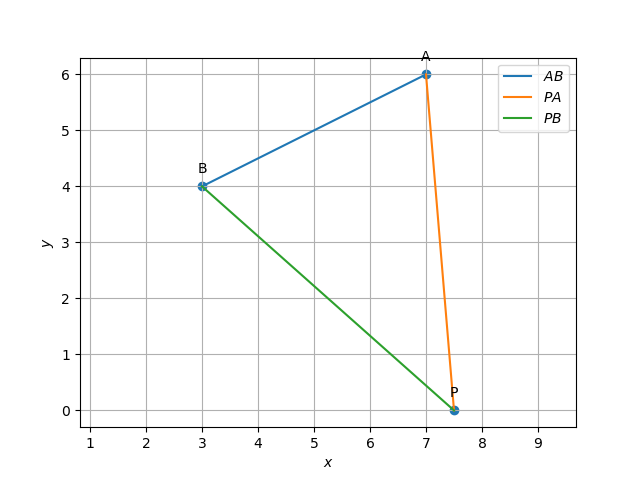
\includegraphics[width=1\columnwidth]{line.png}
\caption{Plot of Quadrilateral}
\end{figure}

\section{Solution}
\begin{flushleft}


Let angle in the ratio 3:5:9:13 be a,b,c,d\\
\vspace{0.25cm}
Let a=3x,b=5x,,c=9x,d=13x\\
\vspace{0.25cm}
where x is any number\\
\vspace{0.25cm}
We know that\\
\vspace{0.25cm}
Sum of angle of quadrilateral is 360\textdegree\\
\vspace{0.25cm}
a+b+c+d=360$\textdegree$   [Angle sum property of quadrilateral]\\
\vspace{0.25cm}
3x+5x+9x+13x=360\textdegree \\
\vspace{0.25cm}
30x=360\textdegree\\
\vspace{0.25cm}
x=360/30\\
\vspace{0.25cm}
x=12$\textdegree$\\
\vspace{0.25cm}
Hence the angles of Quadrilateral are\\
\vspace{0.25cm}
a=3x=3×12=36\textdegree\\
\vspace{0.25cm}
b=5x=5×12=60\textdegree\\
\vspace{0.25cm}
c=9x=9×12=108\textdegree\\
\vspace{0.25cm}
d=13x=13×12=156\textdegree
\end{flushleft}




\section{Software}
\begin{flushleft}
Download the codes given in the link below and execute them.\\
\end{flushleft}

\begin{table}[h]
\centering
\begin{tabular}{|c|} \hline
\rule{0pt}{10pt} 
https://github.com/sureshoye/line-assignment/blob \\
/main/codes/line.py\\
\\\hline
 \end{tabular}
\end{table}




\section{Conclusion}
\begin{flushleft}
The angles of Quadrilateral are\\
\vspace{0.25cm}
a=3x=3×12=36\textdegree\\
\vspace{0.25cm}
b=5x=5×12=60\textdegree\\
\vspace{0.25cm}
c=9x=9×12=108\textdegree\\
\vspace{0.25cm}
d=13x=13×12=156\textdegree
\end{flushleft}
\endcenter
\end{document}
\fi

\item 
\label{chapters/9/8/1/2}
\iffalse
 

\def\mytitle{MATRICES USING PYTHON}
\def\myauthor{THOUTU RAHUL RAJ}
\def\contact{rdj4648@gmail.com}
\def\mymodule{Future Wireless Communication (FWC)}
\documentclass[10pt, a4paper]{article}
\usepackage[a4paper,outer=1.5cm,inner=1.5cm,top=1.75cm,bottom=1.5cm]{geometry}
\twocolumn
\usepackage{graphicx}
\graphicspath{{./images/}}
\usepackage[colorlinks,linkcolor={black},citecolor={blue!80!black},urlcolor={blue!80!black}]{hyperref}
\usepackage[parfill]{parskip}
\usepackage{lmodern}
\usepackage{amsmath,amsfonts,amssymb,amsthm}
\usepackage{tikz}
	\usepackage{physics}
%\documentclass[tikz, border=2mm]{standalone}
\usepackage{karnaugh-map}
%\documentclass{article}
\usepackage{tabularx}
\usepackage{circuitikz}
\usetikzlibrary{calc}
\usepackage{amsmath}
\usepackage{amssymb}
\renewcommand*\familydefault{\sfdefault}
\usepackage{watermark}
\usepackage{lipsum}
\usepackage{xcolor}
\usepackage{listings}
\usepackage{float}
\usepackage{titlesec}
\providecommand{\norm}[1]{\left\lVert#1\right\rVert}
\providecommand{\sbrak}[1]{\ensuremath{{}\left[#1\right]}}
\providecommand{\lsbrak}[1]{\ensuremath{{}\left[#1\right.}}
\providecommand{\rsbrak}[1]{\ensuremath{{}\left.#1\right]}}
\providecommand{\brak}[1]{\ensuremath{\left(#1\right)}}
\providecommand{\lbrak}[1]{\ensuremath{\left(#1\right.}}
\providecommand{\rbrak}[1]{\ensuremath{\left.#1\right)}}
\providecommand{\cbrak}[1]{\ensuremath{\left\{#1\right\}}}
\providecommand{\lcbrak}[1]{\ensuremath{\left\{#1\right.}}
\providecommand{\rcbrak}[1]{\ensuremath{\left.#1\right\}}}
\newcommand{\myvec}[1]{\ensuremath{\begin{pmatrix}#1\end{pmatrix}}}
\let\vec\mathbf
\providecommand{\mtx}[1]{\mathbf{#1}}
\titlespacing{\subsection}{1pt}{\parskip}{3pt}
\titlespacing{\subsubsection}{0pt}{\parskip}{-\parskip}
\titlespacing{\paragraph}{0pt}{\parskip}{\parskip}
\newcommand{\figuremacro}[5]

\begin{document}

\title{\mytitle}
\author{\myauthor\hspace{1em}\\\contact\\FWC22008\hspace{6.5em}IITH\hspace{0.5em}\mymodule\hspace{6em}ASSIGN-4}
\date{}
	\maketitle
		
	\tableofcontents
\vspace{5mm}
\fi
If diagonals of a parallelogram are equal then show that it is a rectangle.

	\begin{figure}[!h]
		\centering
		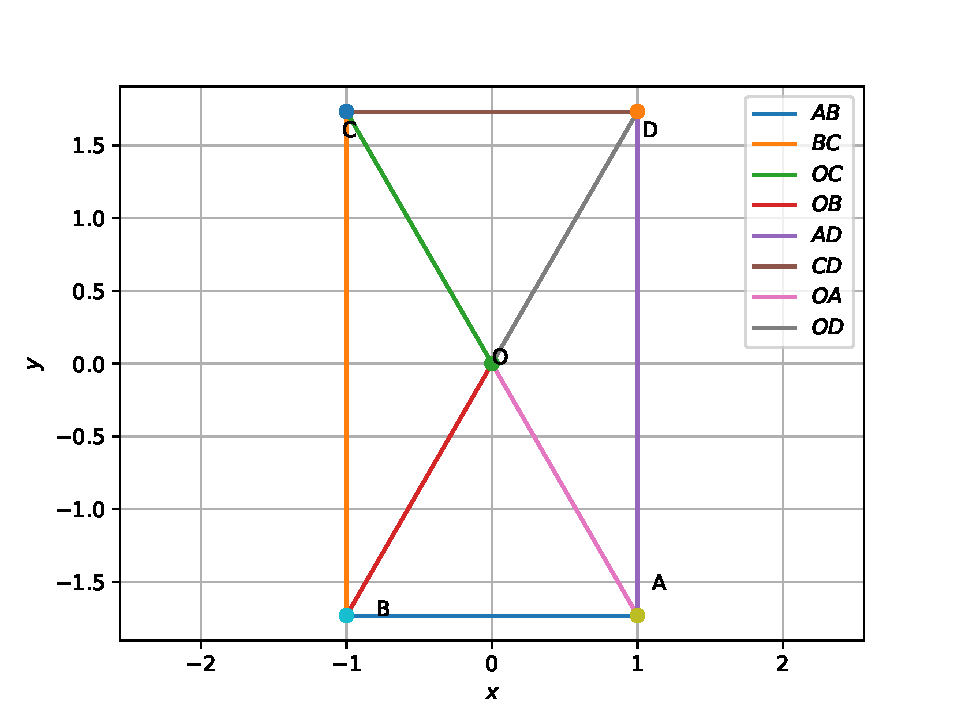
\includegraphics[width=\columnwidth]{chapters/9/8/1/2/fig.pdf}
     %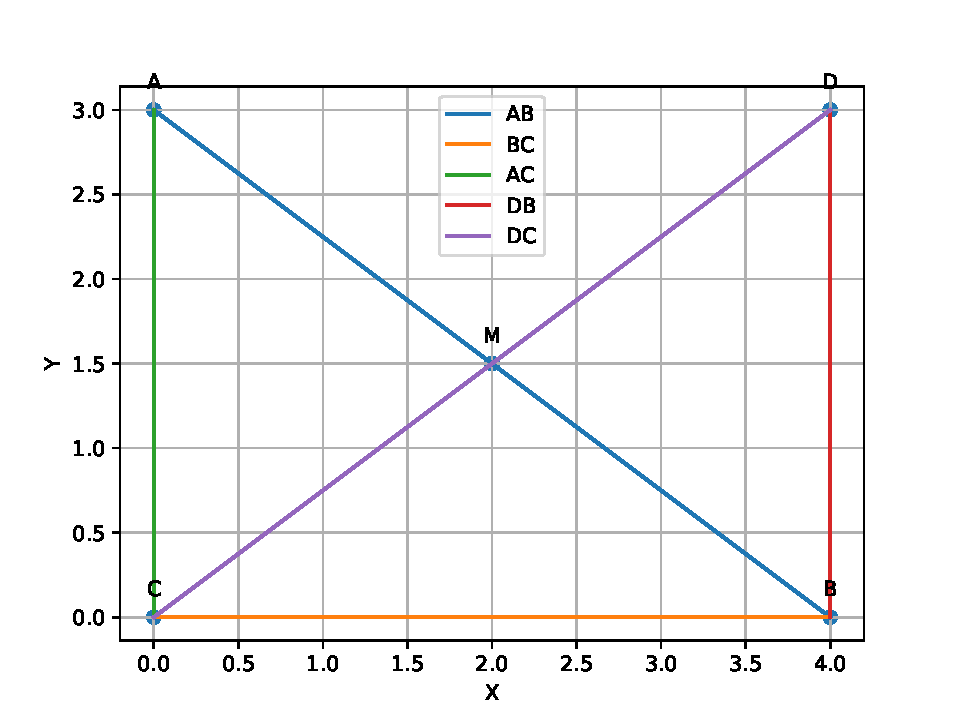
\includegraphics[scale=0.5]{fig.pdf} 
		\caption{}
		\label{fig:9/8/1/2}
  	\end{figure}
	\solution 
   See Fig. 
		\ref{fig:9/8/1/2}.
   From 
	  \eqref{eq:two-pgm}, 
\begin{align}
	  \label{eq:two-pgm-def} 
 \vec{B} - \vec{A}= \vec{C}-\vec{D}
 \\
\implies  \vec{B} - \vec{C}= \vec{A}-\vec{D}
	\end{align}
	Also, it is given that the diagonals of $ABCD$ are equal.  Hence, 
\begin{align}
	\norm{\vec{C} - \vec{A}}^2&= \norm{\vec{D}-\vec{B}}^2
 \\
	\implies 
	\norm{(\vec{C}-\vec{B}) + (\vec{B}-\vec{A})}^2 &= \norm{(\vec{D}-\vec{C}) + (\vec{C}-\vec{B}}^2
\end{align}
which can be expressed as
\begin{multline}
	\norm{\vec{C}-\vec{B}}^2 + \norm{\vec{B}-\vec{A}}^2 + 2(\vec{C}-\vec{B})^{\top} (\vec{B}-\vec{A}) 
	\\
	= \norm{\vec{D}-\vec{C}}^2 + \norm{\vec{C}-\vec{B}}^2+2(\vec{D}-\vec{C})^{\top} (\vec{C}-\vec{B}) 
\end{multline}
which, can be simplified to obtain 
\begin{align}
	(\vec{C}-\vec{B})^{\top} (\vec{B}-\vec{A})&=(\vec{D}-\vec{C})^{\top} (\vec{C}-\vec{B}) 
\end{align}
since 
\begin{align}
\norm{\vec{D}-\vec{C}} =   
\norm{\vec{B}-\vec{A}}   
\end{align}
yielding 
\begin{align}
	(\vec{A}-\vec{B})^{\top} (\vec{B}-\vec{C})=\vec{0}
\end{align}
	  from \eqref{eq:two-pgm-def}.  

\item 
\label{chapters/9/8/1/3}
\iffalse
\documentclass[a4paper,12pt,twocolumn]{article}
\usepackage{graphicx}
\usepackage[margin=0.5in]{geometry}
\usepackage[cmex10]{amsmath}
\usepackage{array}
\usepackage{gensymb}
\usepackage{booktabs}
\title{Line Assignment}

\author{Ravi Sumanth Muppana- FWC22003}
\date{September 2022}
\providecommand{\norm}[1]{\left\lVert#1\right\rVert}
\providecommand{\abs}[1]{\left\vert#1\right\vert}
\let\vec\mathbf
\newcommand{\myvec}[1]{\ensuremath{\begin{pmatrix}#1\end{pmatrix}}}	
\newcommand{\mydet}[1]{\ensuremath{\begin{vmatrix}#1\end{vmatrix}}}
\providecommand{\brak}[1]{\ensuremath{\left((#1\right)}}
\begin{document}
\maketitle
\section{Problem:}
\fi
Show that if the diagonals of a quadrilateral bisect each other at right angles, then it is a rhombus.
\begin{figure}[!h]
	\centering
	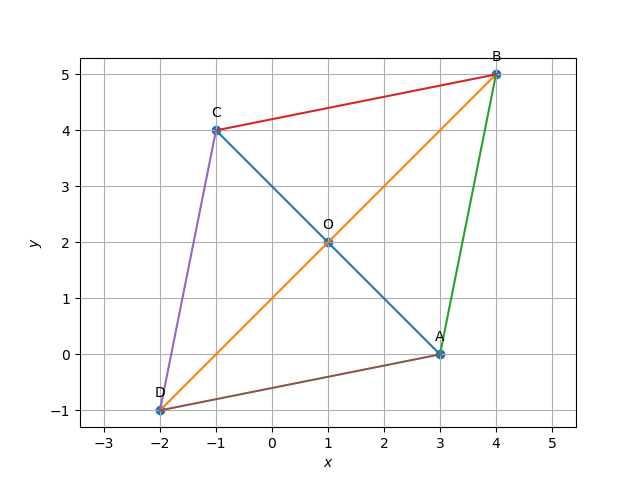
\includegraphics[width=\columnwidth]{chapters/9/8/1/3/figs/rhombus.png}
	\caption{Rhombus}
	\label{fig:9/8/1/3}
\end{figure}
\\
\solution See Fig. 
	\ref{fig:9/8/1/3}.
\iffalse
\maketitle
\section{Solution:}
\subsection{Theory:}
\fi
From the given information,
\begin{align}
	\label{eq:9/8/1/3-mid}
	\frac{\vec{B}+\vec{D}}{2}
	&=	
	\frac{\vec{A}+\vec{C}}{2}
	\\
	\brak{\vec{B}-\vec{D}}^{\top}&
	\brak{\vec{A}-\vec{C}} = 0
	\label{eq:9/8/1/3-orth}
\end{align}
From 
	\eqref{eq:9/8/1/3-mid},
\begin{align}
	\vec{B}-\vec{A}
	=	
	\vec{C}-\vec{D}
	\label{eq:9/8/1/3-pgm}
\end{align}
which, from  
	  \eqref{eq:two-pgm}, 
is the definition of  a parallelogram.
Further, substituting
\begin{align}
	\vec{B}-\vec{D} &= \brak{\vec{B}-\vec{A}} +  
	\brak{\vec{A}-\vec{D}}
	\\
	\vec{A}-\vec{C} &= \brak{\vec{A}-\vec{B}} +  
	\brak{\vec{B}-\vec{C}}
\end{align}
in 
	\eqref{eq:9/8/1/3-orth},  
\begin{multline}
	\sbrak{\brak{\vec{B}-\vec{A}} +  
	\brak{\vec{A}-\vec{D}}}^{\top}
	\sbrak{ \brak{\vec{A}-\vec{B}} +  
	\brak{\vec{B}-\vec{C}}} = 0
	\\
	\implies 
-\norm{\vec{B}-\vec{A}}^2 + \brak{\vec{B}-\vec{A}}^{\top}\brak{\vec{B}-\vec{C}} + 
\\
	\brak{\vec{A}-\vec{D}}^{\top}\brak{\vec{A}-\vec{B}} + 
\brak{\vec{A}-\vec{D}}^{\top}
\brak{\vec{B}-\vec{C}} = 0
	\label{eq:9/8/1/3-org}
\end{multline}
From
	\eqref{eq:9/8/1/3-pgm},
\begin{align}
	\vec{B}-\vec{C}
	=	
	\vec{A}-\vec{D}
	\\
	\implies \brak{\vec{B}-\vec{A}}^{\top}\brak{\vec{B}-\vec{C}} +
	 \brak{\vec{A}-\vec{D}}^{\top}\brak{\vec{A}-\vec{B}} =\vec{0}
	\label{eq:9/8/1/3-orth-pf}
\end{align}
and 
\begin{align}
\brak{\vec{A}-\vec{D}}^{\top}
\brak{\vec{B}-\vec{C}} = \norm{\vec{B}-\vec{C}}^2
	\label{eq:9/8/1/3-orth-eq}
\end{align}
Substituting from

	\eqref{eq:9/8/1/3-orth-pf}
and
	\eqref{eq:9/8/1/3-orth-eq}
in
	\eqref{eq:9/8/1/3-org},

\begin{align}
\norm{\vec{A}-\vec{B}}^{2}
= \norm{\vec{B}-\vec{C}}^2
\end{align}
which means that the adjacent sides of the parallelogram are equal. Thus, the quadrilateral is a rhombus
\iffalse


Since
Let us assume two vectors $\vec{C}-\vec{B}-\vec{A}$ and $\vec{C}-\vec{B}$ for sides $BA$ and $CB$. The diagonals $AC,BD$ are the addition and subtraction of the two vectors:
\begin{align}
	&\vec{(B-A)} = \vec{C}-\vec{B}-\vec{A}\\
	&\vec{(C-B)} = \vec{C}-\vec{B}\\
	&\vec{(C-A)} = \vec{(C-B)} +\vec{(B-A)}\\
	&\vec{(C-A)} = \vec{b+a}\\
	&\vec{(D-B)} = \vec{b-a}\\
\end{align}
%\subsection{Mathematical Calculation:}
Let the two diagonals be $\vec{a+b}$, $\vec{b-a}$. Since the diagonals are at right angle to each other,
\begin{align}
&0 = \vec{(a+b)^T}\vec{(b-a)}\\	
&||\vec{C}-\vec{B}||^2 - ||\vec{C}-\vec{B}-\vec{A}||^2 = 0\\
&||\vec{C}-\vec{B}|| = ||\vec{C}-\vec{B}-\vec{A}||\\
\end{align}
Hence, the two sides of the quadrilateral are equal. We need to prove the third side is also equal.
Now,
In triangle BOA and AOD;
\begin{align}
	&\vec{B-O} = \vec{p}\\
	&\vec{D-O} = \vec{-p}\\
	&\vec{A-O} = \vec{r}\\
\end{align}
\begin{align}
	&\vec{C}-\vec{B}-\vec{A} = \vec{(B-O)} - \vec{(A-O)}\\ 
	&\vec{d} = \vec{(D-O)} - \vec{(A-O)}\\
&||\vec{C}-\vec{B}-\vec{A}||^2 = ||\vec{p}||^2 + ||\vec{r}||^2 - 2\vec{p^Tr}\\
&||\vec{d}||^2 = ||\vec{-p}||^2 + ||\vec{r}||^2 + 2\vec{p^Tr}\\
\end{align}
The terms $\vec{p^Tr}$ is equal to zero as they is perpendicular.Therefore,
\begin{align}
	&||\vec{C}-\vec{B}-\vec{A}||^2 = ||\vec{p}||^2 + ||\vec{r}||^2\\
	&||\vec{d}||^2 = ||\vec{p}||^2 + ||\vec{r}||^2\\
	&Clearly, ||\vec{C}-\vec{B}-\vec{A}|| = ||\vec{d}||\\
\end{align}
Hence, all three sides are equal, it's a parallelogram. A parallelogram with it's diagonals as perpendicular bisectors is a rhombus.
\fi
\iffalse
\section{Construction:}
Consider any  three vertices of the rhombus. Using the vertices, find the midpoint of the diagonals, then find the fourth point using the midpoint and remaining vertex. 
\begin{table}[h]
	\centering
\setlength\extrarowheight{2pt}
	\begin{tabular}{|c|c|c|}
		\hline
		\textbf{variable} & \textbf{length/point} & \textbf{Description}\\
		\hline
		A & [3,0] & Vertex A\\
		\hline
		B & [4,5] & Vertex B\\
		\hline
		C & [-1,4] & Vertex C\\
		\hline                   
		D & [D-x,D-y] & Vertex D\\
		\hline
		M & (A+B)/2 & midpoint\\
		\hline
		(D-x,D-y) & (2*M[0]-B[0],2*M[1]-B[1]) & vertex of D\\
		\hline
	\end{tabular}
\end{table}

\end{document}
\fi

\item 
\iffalse
\documentclass[journal,12pt,twocolumn]{article}
\usepackage{graphicx}
\usepackage[none]{hyphenat}
\usepackage[margin=0.5in]{geometry}
\usepackage[cmex10]{amsmath}
\usepackage{array}
\usepackage{booktabs}
\usepackage{gensymb}
\usepackage{textcomp}
\title{\textbf{Line Assignment}}
\author{Manideep Parusha - FWC22004}
\date{\today}

\providecommand{\norm}[1]{\left\lVert#1\right\rVert}
\providecommand{\abs}[1]{\left\vert#1\right\vert}
\let\vec\mathbf
\newcommand{\myvec}[1]{\ensuremath{\begin{pmatrix}#1\end{pmatrix}}}
\newcommand{\mydet}[1]{\ensuremath{\begin{vmatrix}#1\end{vmatrix}}}
\providecommand{\brak}[1]{\ensuremath{\left(#1\right)}}

\begin{document}

\maketitle
\section*{Problem}
\fi
Show that the diagonals of a square are equal and bisect each other at right angles.
\solution This is obvious from Problems
\eqref{chapters/9/8/1/2}
and
\eqref{chapters/9/8/1/3}.

\iffalse
\section*{Solution}

\begin{figure}[h]
\centering
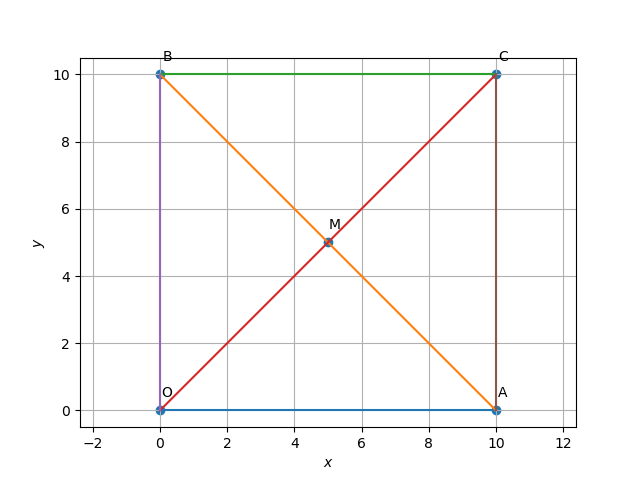
\includegraphics[width=\columnwidth]{figs/sq_plot.png}
\caption{Square generated using python}
\label{fig:sq_py}
\end{figure}

\subsection*{Construction}
Inputs taken for the construction of the Square is 'a' , which is the side length of the square.
\begin{table}[h]
	\centering
\setlength\extrarowheight{2pt}
	\begin{tabular}{|c|c|c|}
		\hline
		\textbf{Symbol} & \textbf{Value} & \textbf{Description} \\
		\hline
		a & 10 & length of OA\\
		\hline
		O & (0,0) & point O\\
		\hline
		A & (a,0) & point A\\
		\hline
		B & (0,a) & point B\\
		\hline
		C & A+B & point C\\
		\hline
		M & $\frac{C}{2}$ & point M\\
		\hline
	\end{tabular}
\end{table}


Let OABC is a Square. Length of all sides are equal for a square and all interior angles equal to 90\degree.
O at the origin and vectors A, B \& C represent other vertices of the square.
\begin{align}
	\norm{\boldsymbol{OA}} = \norm{\boldsymbol{OB}} = \norm{\boldsymbol{BC}} = \norm{\boldsymbol{AC}} \\
\angle OAC = \angle OBC = \angle BCA = \angle AOB = 90\degree
\label{eq-1}
\end{align}
Here, $D_1$ and $D_2$ are the diagonals of the square and we can compute $D_1$ and $D_2$ as
\begin{equation}
	\boldsymbol{D_1 = (A + B) } \\
	\label{D1eq}
\end{equation}
\begin{equation}
	\boldsymbol{D_2 = (A - B) }
	\label{D2eq}
\end{equation}

To prove that the diagonals of the square are equal, we can find the length of the two diagonals and compare. Hence,
\begin{equation}
\norm {\boldsymbol{D_1}}  = \norm {\boldsymbol{A + B}}\\
	\label{D1_len}
\end{equation}
\begin{equation}
\norm {\boldsymbol{D_2}}  = \norm {\boldsymbol{A - B}}
	\label{D2_len}
\end{equation}
For finding length of $D_1$, we can write from equation \eqref{D1_len},  
\begin{align}
	\norm{\boldsymbol{A + B}} = \sqrt{\norm{\boldsymbol{A}}^2 + \norm{\boldsymbol{B}}^2 + 2\boldsymbol{A}^T\boldsymbol{B}}
	\label{extend_D1}
\end{align}
But, for a square we know that length of all sides are equal.
\begin{equation}
	\norm {\boldsymbol{A}} = \norm{\boldsymbol{B}}
	\label{equal_sides}
\end{equation}
and, the angle between two adjacent sides is 90\degree. The dot product of two vectors which are seperated by 90\degree angle is always '0'. 
\begin{equation}
	\boldsymbol{A}^T\boldsymbol{B} = 0 
	\label{dot_product_is_0}
\end{equation}
So the equation \eqref{extend_D1} becomes 
\begin{align}
	\norm {\boldsymbol{A + B}} = \sqrt{2}\norm{\boldsymbol{A}}\\
	\norm {\boldsymbol{D_1}} = \sqrt{2}\norm{\boldsymbol{A}} 
	\label{D1_length}
\end{align}
Similarly, for finding the length of $D_2$ 
\begin{align}
	\norm {\boldsymbol{A - B}} = \sqrt{\norm{\boldsymbol{A}}^2 + \norm{\boldsymbol{B}}^2 - 2\boldsymbol{A}^T\boldsymbol{B}}
\end{align}
But, from \eqref{equal_sides} and \eqref{dot_product_is_0}
\begin{align}
	\norm {\boldsymbol{A - B}} = \sqrt{2}\norm{\boldsymbol{A}}\\
	\norm {\boldsymbol{D_2}} = \sqrt{2}\norm{\boldsymbol{A}} 
	\label{D2_length}
\end{align}
So, from the equations \eqref{D1_length} and \eqref{D2_length}, we can say that the lengths of diagonals $\boldsymbol{D_1}$ and $\boldsymbol{D_2}$ are equal 
\begin{equation}
	\norm{\boldsymbol{D_1}} = \norm{\boldsymbol{D_2}}
\end{equation}





We know that, if the dot product of two vectors is zero then the vectors are perpendicular to each other. \\
So, by taking the dot product of $\boldsymbol{D_1}$ and $\boldsymbol{D_2}$ 
\begin{align}
	\boldsymbol{D_1.D_2} = \boldsymbol{D_1}^T \boldsymbol{D_2} \\
	\boldsymbol{D_1.D_2} = (\boldsymbol{A + B})^T(\boldsymbol{A - B})\\
	\boldsymbol{D_1.D_2} = \norm{\boldsymbol{A}}^2 - \norm{\boldsymbol{B}}^2
\end{align}	
From the equation \eqref{equal_sides}, 
\begin{align}
	\boldsymbol{D_1.D_2} = \norm{\boldsymbol{A}}^2 - \norm{\boldsymbol{A}}^2 \\
	\boldsymbol{D_1.D_2} = 0 
\end{align}	
as the dot product of the diagonals is equal to 0, we can say that both diagonals are perpendicular to each other. \\

Let diagonals $\boldsymbol{D_1}$ and $\boldsymbol{D_2}$ intersect at a point $\boldsymbol{M}$. We have to prove that $\boldsymbol{M}$ is the mid point of $\boldsymbol{D_1}$ and $\boldsymbol{D_2}$, in order to say that both diagonals bisect eachother.
\begin{align}
	\boldsymbol{OM} = x \boldsymbol{D_1}\\
	\boldsymbol{MA} = y \boldsymbol{D_2}
\end{align}
From the equations \eqref{D1eq} and \eqref{D2eq}, the above equations can be written as
\begin{align}
	\boldsymbol{OM} = x\boldsymbol{A + B}\\
	\boldsymbol{MA} = y\boldsymbol{A - B}
\end{align}
Now, if we consider
\begin{align}
	\boldsymbol{OA} = \boldsymbol{OM} + \boldsymbol{MA}\\
	\boldsymbol{A} = x(\boldsymbol{A+B}) + y(\boldsymbol{A-B})\\
	\boldsymbol{A} = x\boldsymbol{A} + x\boldsymbol{B} + y\boldsymbol{A} - y\boldsymbol{B}\\
	\boldsymbol{A} = (x+y)\boldsymbol{A} + (x-y)\boldsymbol{B}
\end{align}
Equating the co-efficient of $\boldsymbol{A}$ and $\boldsymbol{B}$, we get
\begin{align}
	x + y = 1 , x - y = 0\\
	2x = 1\\
	x = \frac{1}{2}\\
	y = \frac{1}{2}
\end{align}

now we can say that
\begin{align}
	\boldsymbol{OM} = \frac{1}{2} \boldsymbol{D_1}\\
	\boldsymbol{MA} = \frac{1}{2} \boldsymbol{D_2}
\end{align}
Hence, M is the mid point of diagonals $D_1$ and $D_2$ and we can say that both diagonals bisect eachother. \\

we have proved that diagonals of a square are equal in length and bisect eachother at right angles.





\end{document}
\fi

\item 
\item 
\iffalse
\documentclass[a4paper,12pt,twocolumn]{article}
\usepackage{graphicx}
\usepackage[margin=0.5in]{geometry}
\usepackage[cmex10]{amsmath}
\usepackage{array}
\usepackage{gensymb}
\usepackage{booktabs}
\usepackage{tabularx}
\title{Line Assignment}

\author{Ginna Shreyani- FWC22006}
\date{September 2022}
\providecommand{\norm}[1]{\left\lVert#1\right\rVert}
\providecommand{\abs}[1]{\left\vert#1\right\vert}
\let\vec\mathbf
\newcommand{\myvec}[1]{\ensuremath{\begin{pmatrix}#1\end{pmatrix}}}	
\newcommand{\mydet}[1]{\ensuremath{\begin{vmatrix}#1\end{vmatrix}}}
\providecommand{\brak}[1]{\ensuremath{\left((#1\right)}}
\begin{document}
\maketitle
\section{Problem:}
\fi
Diagonal AC of a parallelogram ABCD bisects $\angle{A}$ in Fig \eqref{fig:9/8/1/6}. Show that 
\begin{enumerate}
	\item	it bisects $\angle{C}$ also
	\item $ABCD$ is a rhombus
\end{enumerate}
\begin{figure}[!h]
	\centering
	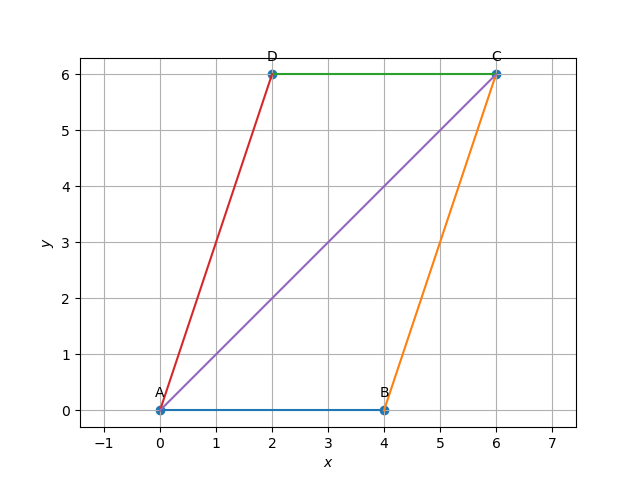
\includegraphics[width=\columnwidth]{chapters/9/8/1/6/figs/parallel.png}
	\caption{}
	\label{fig:9/8/1/6}
\end{figure}
\solution  
\iffalse
are given by 
\begin{proof}
Any point on the angle bisector is equidistant from the lines.  
\end{proof}
\fi	
%\item ({\em Reflection }) Assuming that straight lines work as a plane mirror for a point, find the image of the point $\vec{P}=\myvec{1\\2}$ in the line 
%%
\iffalse
\maketitle
\section{Construction:}
\begin{tabularx}
{0.5\textwidth}{
|>
{\raggedright\arraybackslash}X
|>
{\centering\arraybackslash}X
|>
{\raggedleft\arraybackslash}X
|}
\hline
 Variable & Point/Length & Description\\
\hline
 A  &  $\myvec{0\\0}$ & Vertex A\\
 \hline
 B & $\myvec{4\\0}$ & Vertex B\\
 \hline
 C & $\myvec{6\\6}$ & Vertex C\\
 \hline
 D & $\myvec{2\\6}$ & Vertex D\\
 \hline
\end{tabularx}
\maketitle
\section{Solution:}
\subsection{Theory:}
Given a diagonal of a parallelogram bisects an angle,we need to prove that the same diagonal bisects the opposite angle of the parallelogram by using vector algebra.\\
\subsection{Mathematical Calculation:}
Here the diagonal joining vertices A and C  can be represented as
\begin{equation}
\vec{C}-\vec{A} = \vec{B}-\vec{A}+\vec{C}-\vec{B}
\end{equation}
The other diagonal joining vertices B and D can be represented as
\begin{equation}
\vec{D-B} = \vec{B}-\vec{C}-\vec{B}-\vec{A}
\end{equation}
$\boldsymbol{(i)}$ Let the $\angle{CAB}$  be $\theta_1$ and the $\angle{DAC}$  be $\theta_2$ and the $\angle{DCA}$  be $\theta_3$ and $\angle{ACB}$ be $\theta_4$\\
Since the diagonal $\vec{C}-\vec{A}$ bisects $\angle{A}$, $\angle{CAB} = \angle{DAC}$,therefore we get $\theta_1=\theta_2$\\
\fi
\begin{enumerate}
	\item From 
    \eqref{eq:angle2d},
\begin{align}
	 \label{eq:9/8/1/6/bis}
	\angle{BAC}
	&= \angle{DAC}
	\\
\implies  \frac{(\vec{A}-\vec{B})^T(\vec{A}-\vec{C})}{\norm{\vec{A}-\vec{B}}\norm{\vec{A}-\vec{C}}}
	& = \frac{(\vec{A}-\vec{D})^T(\vec{A}-\vec{C})}{\norm{\vec{A}-\vec{D}}\norm{\vec{A}-\vec{C}}}
%
%&cos\theta_3 = \frac{\vec{-(B-A)}^T\vec{-(C-A)}}{\vec{||-(B-A)||}.\vec{||-(C-A)||}}\\
%&cos\theta_3 = \frac{\brak{vec{B}-\vec{A}}^T\brak{vec{C}-\vec{A}}}{\vec{||B-A||}.\vec{||C-A||}}\\
%&cos\theta_1 = cos\theta_3\\
%&\theta_1=\theta_3
\end{align}
Also, 
\begin{align}
\cos	\angle{ACD}
	 = \frac{(\vec{C}-\vec{D})^T(\vec{C}-\vec{A})}{\norm{\vec{C}-\vec{D}}\norm{\vec{C}-\vec{A}}}
	 \label{eq:9/8/1/6/cang}
%
\end{align}
From Appendix
	  \ref{eq:two-pgm}, 
  \begin{align}
	  \vec{B}-\vec{A} &= \vec{C} -\vec{D}
	  \\
	  \implies 
	  \frac{(\vec{C}-\vec{D})^T(\vec{C}-\vec{A})}{\norm{\vec{C}-\vec{D}}\norm{\vec{C}-\vec{A}}}
	  &= \frac{(\vec{B}-\vec{A})^T(\vec{C}-\vec{A})}{\norm{\vec{B}-\vec{A}}\norm{\vec{C}-\vec{A}}}
	 \label{eq:9/8/1/6/rh}
  \end{align}
  upon substituting in 
	 \eqref{eq:9/8/1/6/cang}. Thus, from 
	 \eqref{eq:9/8/1/6/cang}
	 and 
	 \eqref{eq:9/8/1/6/bis}, 
\begin{align}
	\angle{BAC}
	= \angle{DAC}
	=
	\angle{ACD}
  \end{align}
  Similarly, it can be shown that 
  \begin{align}
	\angle{ACD}
	=
	\angle{ACB}
  \end{align}
  \item 
  \iffalse
From 
	 \eqref{eq:9/8/1/6/rh}, 
  \begin{align}
	  \frac{(\vec{C}-\vec{D})^T(\vec{C}-\vec{A})}{\norm{\vec{C}-\vec{D}}\norm{\vec{C}-\vec{A}}}
	  &= \frac{(\vec{B}-\vec{A})^T(\vec{C}-\vec{A})}{\norm{\vec{B}-\vec{A}}\norm{\vec{C}-\vec{A}}}
  \end{align}
The equation of the bisector of $\angle BAD$ is given by Appendix  
	\ref{prob:ang-bisect} as
\begin{align}
	 \label{eq:9/8/1/6/ac}
	\frac{\vec{n}_1^{\top}\vec{x} - c_1}{\norm{\vec{n}_1}}
	= 
	\frac{\vec{n}_2^{\top}\vec{x} - c_2}{\norm{\vec{n}_2}}
\end{align}
where the equations of $AB, AD$ are respectively given by 
\begin{align}
	\vec{n}_1^{\top}\vec{x} &= c_1
	\\
	\vec{n}_2^{\top}\vec{x} &= c_2
\end{align}
From 
    \eqref{eq:dir_vec}
    and 
    \eqref{eq:normal_vec}, 
\begin{align}
	 \label{eq:9/8/1/6/orth}
	\vec{n}_1^{\top}\brak{\vec{A}-\vec{B}} &= 0
	\\
	\vec{n}_2^{\top}\brak{\vec{A}-\vec{D}}&= 0
\end{align}
%
From 
	 \eqref{eq:9/8/1/6/ac}, the normal vector of $AC$ is 
\begin{align}
	\frac{\vec{n}_1}{\norm{\vec{n}_1}}
	&- 
	\frac{\vec{n}_2}{\norm{\vec{n}_2}}
	\\
	\implies
	\brak{\frac{\vec{n}_1}{\norm{\vec{n}_1}}
	- 
	\frac{\vec{n}_2}{\norm{\vec{n}_2}}}^{\top}
\brak{\vec{B}-\vec{D}}
	&= 
	\brak{\frac{\vec{n}_1}{\norm{\vec{n}_1}}
	- 
	\frac{\vec{n}_2}{\norm{\vec{n}_2}}}^{\top}
	\sbrak{\brak{\vec{B}-\vec{A}}+
	\brak{\vec{A}-\vec{D}}}
\end{align}
which can be expressed as 
\begin{align}
	{\frac{\vec{n}_1^{\top}}{\norm{\vec{n}_1}}}\brak{\vec{A}-\vec{D}}
	- 
	\frac{\vec{n}_2^{\top}}{\norm{\vec{n}_2}}
	\brak{\vec{B}-\vec{A}}
\end{align}
upon substituting from 
	 \eqref{eq:9/8/1/6/orth}.
	 \fi

\end{enumerate}


\iffalse
Therefore,$\angle{CAB}=\angle{DAC}=\angle{DCA}$\\
Similarly, applying the same process to $\angle{DAC}$ and $\angle{ACB}$, we get $\theta_2=\theta_4$ and as result $\angle{DAC}=\angle{ACB}$.\\
Therefore, $\angle{DCA} = \angle{ACB}$\\
Since both the angles $\angle{DCA}$ and $\angle{ACB}$ are equal, we can conclude that the diagonal $\vec{C}-\vec{A}$ bisects the $\angle{C}$.\\ 
\end{document}
\fi

\item 
\iffalse
\def\mytitle{MATRICES USING PYTHON}
\def\myauthor{Ballepu Dheeraj Kumar}
\def\contact{dheeraj.ballepu@gmail.com}
\def\mymodule{Future Wireless Communication (FWC)}
\documentclass[10pt, a4paper]{article}
\usepackage[a4paper,outer=1.5cm,inner=1.5cm,top=1.75cm,bottom=1.5cm]{geometry}
\twocolumn
\usepackage{graphicx}
\graphicspath{{./images/}}
\usepackage[colorlinks,linkcolor={black},citecolor={blue!80!black},urlcolor={blue!80!black}]{hyperref}
\usepackage[parfill]{parskip}
\usepackage{lmodern}
\usepackage{amsmath,amsfonts,amssymb,amsthm}
\usepackage{tikz}
	\usepackage{physics}
%\documentclass[tikz, border=2mm]{standalone}
\usepackage{karnaugh-map}
%\documentclass{article}
\usepackage{tabularx}
\usepackage{circuitikz}
\usetikzlibrary{calc}
\usepackage{amsmath}
\usepackage{amssymb}
\renewcommand*\familydefault{\sfdefault}
\usepackage{watermark}
\usepackage{lipsum}
\usepackage{xcolor}
\usepackage{listings}
\usepackage{float}
\usepackage{titlesec}
\providecommand{\norm}[1]{\left\lVert#1\right\rVert}
\providecommand{\sbrak}[1]{\ensuremath{{}\left[#1\right]}}
\providecommand{\lsbrak}[1]{\ensuremath{{}\left[#1\right.}}
\providecommand{\rsbrak}[1]{\ensuremath{{}\left.#1\right]}}
\providecommand{\brak}[1]{\ensuremath{\left(#1\right)}}
\providecommand{\lbrak}[1]{\ensuremath{\left(#1\right.}}
\providecommand{\rbrak}[1]{\ensuremath{\left.#1\right)}}
\providecommand{\cbrak}[1]{\ensuremath{\left\{#1\right\}}}
\providecommand{\lcbrak}[1]{\ensuremath{\left\{#1\right.}}
\providecommand{\rcbrak}[1]{\ensuremath{\left.#1\right\}}}
\newcommand{\myvec}[1]{\ensuremath{\begin{pmatrix}#1\end{pmatrix}}}
\let\vec\mathbf
\providecommand{\mtx}[1]{\mathbf{#1}}
\titlespacing{\subsection}{1pt}{\parskip}{3pt}
\titlespacing{\subsubsection}{0pt}{\parskip}{-\parskip}
\titlespacing{\paragraph}{0pt}{\parskip}{\parskip}
\newcommand{\figuremacro}[5]

\begin{document}

\title{\mytitle}
\author{\myauthor\hspace{1em}\\\contact\\FWC22008\hspace{6.5em}IITH\hspace{0.5em}\mymodule\hspace{6em}ASSIGN-4}
\date{}
	\maketitle
		
	\tableofcontents
\vspace{5mm}
   \section{Problem}
   \fi
$ABCD$ is a rhombus. Show that the diagonal $AC$ bisects angle $A$ as well as angle $C$ and diagonal $BD$ bisects angle $B$ as well as angle $D$. 
\\
\solution
\iffalse
}
   \section{Solution}
   \textbf{Theory:}\\

   Given  ABCD is a rhombus \\ 
  

\textbf{To Prove:} Diagonals bisects angles\\
\fi
%
For the rhombus in Fig. 
		\ref{fig:9/8/1/7},
 	\begin{figure}
		\centering
 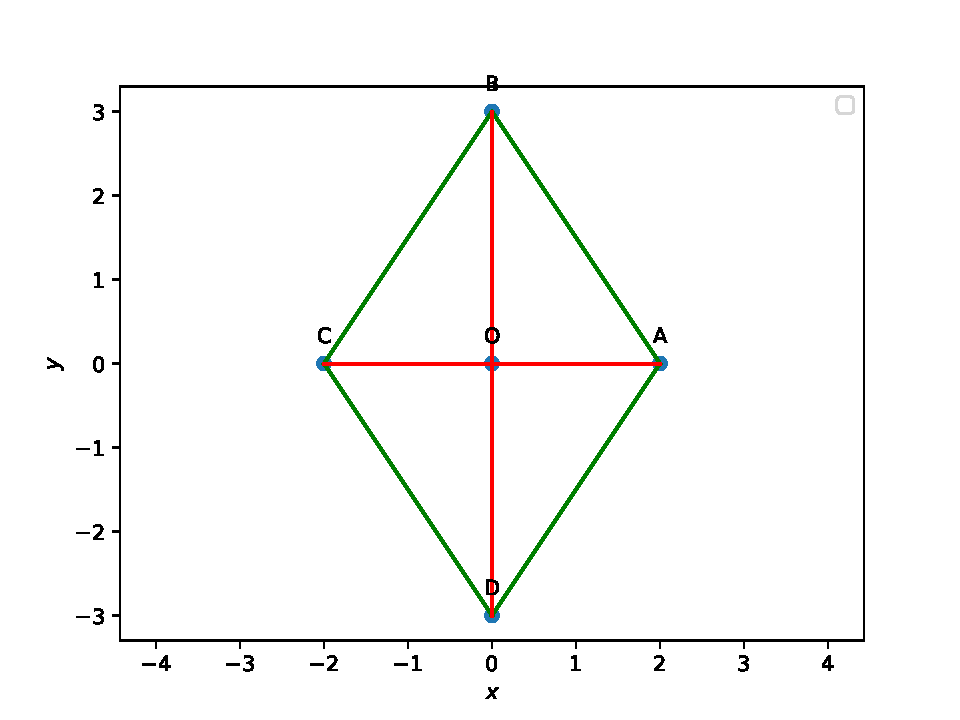
\includegraphics[width=\columnwidth]{chapters/9/8/1/7/figs/fig5.pdf} 
		\caption{}
		\label{fig:9/8/1/7}
  	\end{figure}
\begin{align}
		\label{eq:9/8/1/7}
		\begin{split}
	\norm{\vec{A}-\vec{B}}&=\norm{\vec{A}-\vec{D}}
\\
	\vec{A}-\vec{B}&=\vec{D}-\vec{C}
		\end{split}
\end{align}
From 
    \eqref{eq:angle2d},
\begin{align}
		\begin{split}
	\cos \angle{BAC}
	&= \frac{(\vec{A}-\vec{B})^T(\vec{A}-\vec{C})}{\norm{\vec{A}-\vec{B}}\norm{\vec{A}-\vec{C}}}
	\\
\cos	\angle{DAC}
	 &= \frac{(\vec{C}-\vec{D})^T(\vec{C}-\vec{A})}{\norm{\vec{C}-\vec{D}}\norm{\vec{C}-\vec{A}}}
		\end{split}
	 \label{eq:9/8/1/8/cang}
%
\end{align}
From 
		\eqref{eq:9/8/1/7}
and
	 \eqref{eq:9/8/1/8/cang}, 
%
	 we obtain
\begin{align}
		\begin{split}
	\cos \angle{BAC}
	=\cos \angle{DAC}
		\end{split}
\end{align}
Thus, $AC$ bisects $\angle A$.  Similarly, the remaining results can be proved.

\item 
\item 
\iffalse
\def\mytitle{PYTHON PROGRAMMING ON MATRICES}
\def\myauthor{K.Pavan Kumar}
\def\contact{r170850@rguktrkv.ac.in}
\def\mymodule{Future Wireless Communication (FWC)}
\documentclass[10pt, a4paper]{article}
\usepackage[a4paper,outer=1.5cm,inner=1.5cm,top=1.75cm,bottom=1.5cm]{geometry}
\twocolumn
\usepackage{graphicx}
\graphicspath{{./images/}}
\usepackage[colorlinks,linkcolor={black},citecolor={blue!80!black},urlcolor={blue!80!black}]{hyperref}
\usepackage[parfill]{parskip}
\usepackage{lmodern}
\usepackage{tikz}
	\usepackage{physics}
\usepackage{tabularx}
\usepackage{enumitem}
\usetikzlibrary{calc}
\usepackage{amsmath}
\usepackage{amssymb}
\renewcommand*\familydefault{\sfdefault}
\usepackage{watermark}
\usepackage{lipsum}
\usepackage{xcolor}
\usepackage{listings}
\usepackage{float}
\usepackage{titlesec}
\providecommand{\mtx}[1]{\mathbf{#1}}
\titlespacing{\subsection}{1pt}{\parskip}{3pt}
\titlespacing{\subsubsection}{0pt}{\parskip}{-\parskip}
\titlespacing{\paragraph}{0pt}{\parskip}{\parskip}


\newcommand{\myvec}[1]{\ensuremath{\begin{pmatrix}#1\end{pmatrix}}}
\let\vec\mathbf
\lstset{
frame=single, 
breaklines=true,
columns=fullflexible
}
\thiswatermark{\centering \put(0,-110.0){
\includegraphics[scale=0.3]{logo.png}} }
\title{\mytitle}
\author{\myauthor\hspace{1em}\\\contact\\FWC22011\hspace{6.5em}IITH\hspace{0.5em}\mymodule\hspace{6em}Matrix:Line}
\date{}
\begin{document}
	\maketitle
	\tableofcontents
	\fi

In parallelogram $ABCD$, two points $\vec{P}$ and $\vec{Q}$ are
taken on diagonal $BD$ such that $DP = BQ$. Show that 
\begin{enumerate}
	\item  $\Delta APD \cong \Delta CQB$         
	\item  $AP = CQ$
	\item $\Delta AQB \cong \Delta CPD$     
	\item  $AQ = CP$   
	\item  $APCQ$ is a parallelogram 
\end{enumerate}
\solution 
See Fig. 
		\ref{fig:9/8/1/9}.
 	\begin{figure}
		\centering
 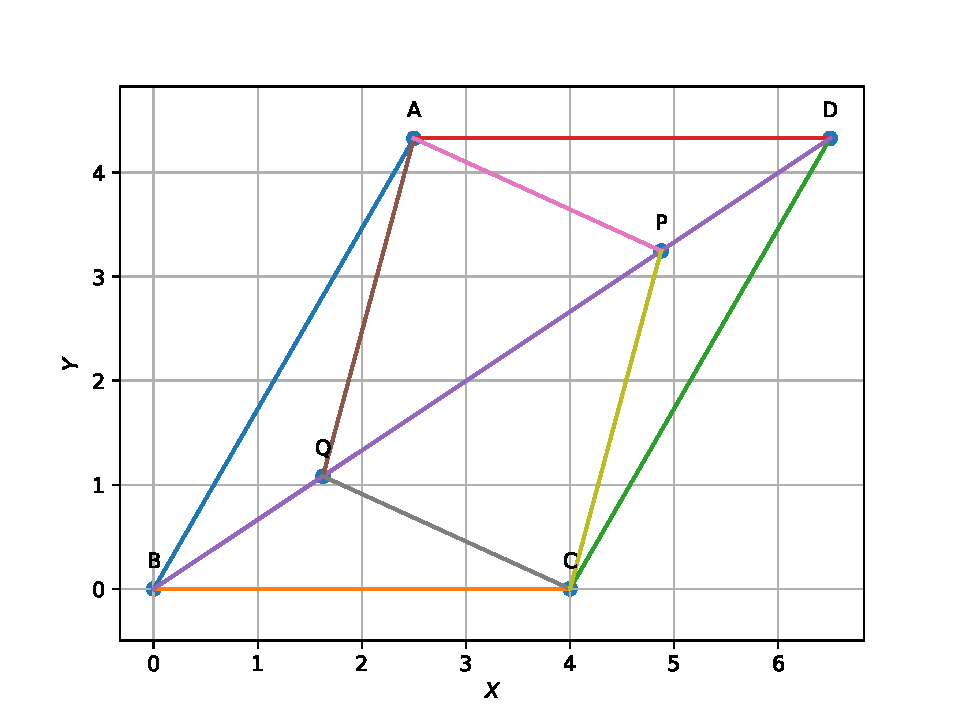
\includegraphics[width=\columnwidth]{chapters/9/8/1/9/figs/output.pdf}
		\caption{}
		\label{fig:9/8/1/9}
  	\end{figure}

\iffalse

\section{Construction}
  	\begin{center}
  Figure of construction
  	\end{center}

   
  \section{Solution}
\begin{center}
The input parameters for this construction are
\begin{tabular}{|c|c|}
	\hline
	\textbf{Symbol}&\textbf{Value}\\
	\hline
	r&5\\
	\hline
	k&3\\
	\hline
    b&4\\
	\hline
	$\theta$&$\frac{pi}{3}$\\
	\hline
\end{tabular}
\end{center}

\begin{align*}
\vec{A}=\begin{pmatrix} r\cos\theta\\ r\sin\theta\ \end{pmatrix} \\
\vec{B}=\begin{pmatrix} 0\\ 0\ \end{pmatrix} \\
\vec{C}=\begin{pmatrix} b\\ 0\ \end{pmatrix} \\
\vec{D}={\vec{A}+\vec{C}-\vec{B}} \\
\vec{P} =  \frac{\vec{B} +K\times \vec{D}}{1+K} \\
\vec{Q} =  \frac{K\times\vec{B} +\vec{D}}{1+K} \\ 
\end{align*}


\textbf{Theorem}\\
A quadrilateral is a parallelogram if a pair of opposite sides
is equal and parallel.

"If two directional vectors are equal,implies their magnitude as well as direction are equal to each other."

Two vectors are parallel if they have the same direction (or) are in exactly opposite directions.

\paragraph{Given} ABCD is a parallelogram.
 ,the two points $\vec{P}$ and $\vec{Q}$ are taken on diagonal BD such that DP = BQ.

\fi
From 
    \eqref{eq:angle2d} and the given information,

\begin{align}
	\vec{A}-\vec{B} &=\vec{D}-\vec{C} \\
	\implies    \vec{A}-\vec{D} &=\vec{B}-\vec{C}\\
	\vec{B}-\vec{Q} &=\vec{P}-\vec{D}
\end{align}

From (1) and (3):
\begin{align}
\begin{split}
    \vec{A}+\vec{C} =\vec{B}+\vec{D}\\
    \vec{P}+\vec{Q} =\vec{B}+\vec{D}
\end{split}
\end{align}

From (4)
\begin{align}
    \vec{A}+\vec{C} =\vec{P}+\vec{Q}
\end{align}

From (5)
\begin{align}
     \implies  \vec{A}-\vec{Q} =\vec{P}-\vec{C}\\
    \vec{A}-\vec{P} =\vec{Q}-\vec{C}
\end{align}


\begin{enumerate}
    \item From (2),(3) and (7)
    \begin{align}
        \Delta APD \cong \Delta CQB
    \end{align}
    
    \item \begin{align}
        Equation (7) \implies AP=CQ
    \end{align}
    
     \item From (1),(3) and (6)
    \begin{align}
        \Delta AQB \cong \Delta CPD
    \end{align}

    \item \begin{align}
        Equation (6) \implies AQ=CP
    \end{align}

     \item Equation (6) and (7) 
      $\implies$  Quadrilateral APCQ is a parallelogram.
\end{enumerate}

\iffalse

\textbf{termux commands :}
\begin{lstlisting}
bash lines.sh............using shell command
\end{lstlisting}
\begin{center}
Below python code realizes the above construction :
\fbox{\parbox{8.5cm}{\url{https://github.com/pavan170850/Fwciith2022/blob/main/matrices/line/code/Line.py}}}
\end{center}
\end{document}
\fi

\item 
\def\mytitle{PARALLELOGRAM}
\def\myauthor{VUNNAVA SRAVANI}
\def\contact{sravani21vunnava@gmail.com}
\def\mymodule{Future Wireless Communication (FWC)}
\documentclass[10pt, a4paper]{article}
\usepackage[a4paper,outer=1.5cm,inner=1.5cm,top=1.75cm,bottom=1.5cm]{geometry}
\twocolumn
\usepackage{setspace}
\doublespacing
\usepackage{graphicx}
\graphicspath{{./images/}}
\usepackage[colorlinks,linkcolor={black},citecolor={blue!80!black},urlcolor={blue!80!black}]{hyperref}
\usepackage[parfill]{parskip}
\usepackage{lmodern}
\usepackage{tikz}
	\usepackage{physics}
%\documentclass[tikz, border=2mm]{standalone}
\usepackage{karnaugh-map}
%\documentclass{article}
\usepackage{tabularx}
\usepackage{circuitikz}
\usetikzlibrary{calc}
\usepackage{amsmath}
\usepackage{amssymb}
\renewcommand*\familydefault{\sfdefault}
\usepackage{watermark}
\usepackage{lipsum}
\usepackage{xcolor}
\usepackage{listings}
\usepackage{float}
\usepackage{titlesec}
\providecommand{\mtx}[1]{\mathbf{#1}}
\titlespacing{\subsection}{1pt}{\parskip}{3pt}
\titlespacing{\subsubsection}{0pt}{\parskip}{-\parskip}
\titlespacing{\paragraph}{0pt}{\parskip}{\parskip}
\newcommand{\figuremacro}[5]{
    \begin{figure}[#1]
        \centering
        \includegraphics[width=#5\columnwidth]{#2}
        \caption[#3]{\textbf{#3}#4}
        \label{fig:#2}
    \end{figure}
}
\newcommand{\myvec}[1]{\ensuremath{\begin{pmatrix}#1\end{pmatrix}}}
\let\vec\mathbf
\lstset{
frame=single, 
breaklines=true,
columns=fullflexible
}

%\thiswatermark{\centering \put(181,-119.0){\includegraphics[scale=0.13]{IIT_logo.png}} }
\title{\mytitle}
\author{\myauthor\hspace{1em}\\\contact\\FWC22012\hspace{6.5em}IITH\hspace{0.5em}\mymodule\hspace{6em}ASSIGN-5}
\date{}
\begin{document}
	\maketitle
	\tableofcontents
   \section{Problem}
  ABCD is a parallelogram and AP and CQ are
perpendiculars from vertices A and C on diagonal
BD . Show that \\
(i) $\Delta APB \cong \Delta CQD$  \\       
(ii) AP = CQ

	   % 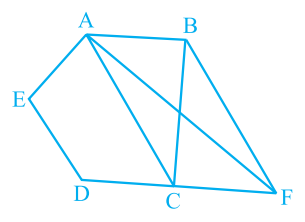
\includegraphics[scale=1.0]{diag_1.png}
   \section{Solution}

The input parameters for this construction are 
\begin{center}
\begin{tabular}{|c|c|}
	\hline
	\textbf{Symbol}&\textbf{Value}\\
	\hline
	b&6\\
	\hline
	r&5\\
	\hline
	$\theta$&$\frac{\pi}{3}$\\
	\hline
\end{tabular}
\begin{center}
$\vec{A}=\myvec{0\\0}$\\
$\vec{D}=\myvec{r\cos\theta \\ r\sin\theta}$\\
$\vec{B}=\myvec{0\\b}$\\
$\vec{C} = \vec{B}+\vec{C}$
\end{center}
\end{center}
\textbf{To Prove:} AP = CQ
		\begin{center}
		The line equation for diagonal BD is $x = \vec{B}+\lambda\vec{m}$
		\\
		where $\vec{m} = \vec{B}-\vec{D}$\\
		
		then,\\
		
		$\vec{P} = \vec{B} - \frac{\vec{m}^T \vec{B}}{\norm{\vec{m}}^2}\vec{m}$
	\\
	
	$\vec{Q} = \vec{B} - \frac{\vec{m}^T \vec{B-C}}{\norm{\vec{m}}^2}\vec{m}$\\
	\end{center}
	
	distance between A and P is $\norm{\vec{A-P}}$\\
	distance between C and Q is $\norm{\vec{C-Q}}$\\
	if $\norm{\vec{A-P}}$ =  $\norm{\vec{C-Q}}$\\
	then AP = CQ..........(1)
	
	\textbf{To Prove:}  $\Delta APB \cong \Delta$ CQD\\
	to prove $\angle {APD}=\angle {CQD}=90^{\circ}$\\
	$\vec{m1} = \vec{A-P}$\\
	$\vec{m2} = \vec{P-B}$\\
	$\theta= \angle {APD}$ \\
	 $\cos\theta$ = $\frac{\vec{m1}^T \vec{m2}}{\norm{\vec{m1}}\norm{\vec{m2}}}$\\
	$\theta = 90^{\circ}, cos\theta$ = 0\\
	$\therefore m1^T m2 = 0$\\
	$\vec{n1} = \vec{C-Q}$\\
	$\vec{n2} = \vec{Q-D}$\\
	$\theta = \angle{CQD}$\\
	$cos\theta$ = $\frac{\vec{n1}^T \vec{n2}}{\norm{\vec{n1}}\norm{\vec{n2}}}$\\
	f $\theta$ = 90$^{\circ}, cos\theta$ = 0\\
	$\therefore n1^T n2 = 0$\\
	\begin{center}
	if 	$m1^T m2 = n1^T n2$ = 0\\
	then, $\angle {APD} = \angle {CQD} = 90^{\circ}$..........(2)\\
	\end{center}
	to prove $\angle {ABP}=\angle {CDQ}$ \\
	$\vec{m2} = \vec{P-B}$\\
	$\vec{m3} = \vec{A-B}$\\
	$\theta1 = \angle {ABP}$\\
	$\theta1 = \cos^-1\frac{\vec{m2} \cdot \vec{m3}}{\norm{\vec{m2}}\norm{\vec{m3}}}$\\
	$\vec{n2} = \vec{C-D}$\\
	$\vec{n3} = \vec{Q-D}$\\
	$\theta2 = \angle {CDQ}$\\
	$\theta2 = \cos^-1\frac{\vec{n2} \cdot \vec{n3}}{\norm{\vec{n2}}\norm{\vec{n3}}}$\\
	\begin{center}
	 		if $\theta1 = \theta2$\\
	 		then $\angle {ABP} = \angle {CQD}$..........(3)
	\end{center}
	\begin{center}
$\therefore$ from (1),(2) and (3)
$\Delta APB \cong \Delta CQD$ 
	\end{center}
The below python code realizes the above construction:	\\
\begin{lstlisting}
https://github.com/sravani21vunnava/sravani21vunnava/blob/main/Matrices_line/codes/matrix_line.py
\end{lstlisting}
 
\section{Construction}
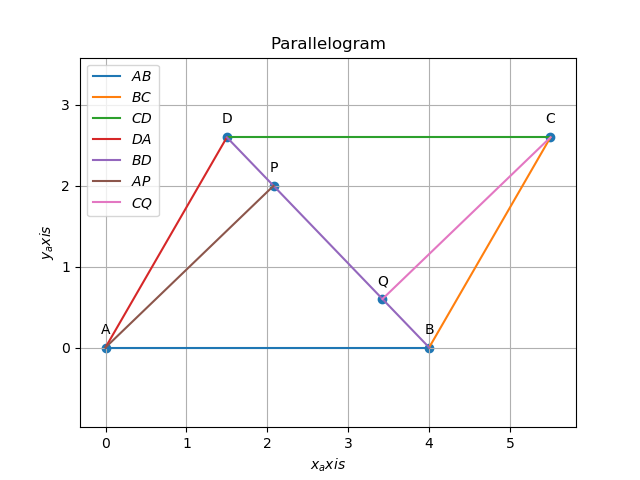
\includegraphics[scale=0.66]{matrix_line.png}
 	
\bibliographystyle{ieeetr}
\end{document}
\item 

\documentclass[10pt, a4paper]{article}
\usepackage[a4paper,outer=1.5cm,inner=1.5cm,top=1.75cm,bottom=1.5cm]{geometry}

\twocolumn
\usepackage{graphicx}
\usepackage{karnaugh-map}
\usepackage{tabularx}
\usepackage{hyperref}
\usepackage[utf8]{inputenc}
\usepackage{amsmath}
\usepackage{physics}
\usepackage{amssymb}

\begin{document}
\title{Assignment-4}
\author{Name:A.Gowri Priya\and Email :  \url{gowripriyaappayyagari@gmail.com}}
%\{ Wireless Communication (FWC)}
\date{}
\maketitle


  \section{Problem}
In  $\Delta$  ABC and  $\Delta$ DEF, AB = DE, AB $\parallel$ DE, BC = EF
and BC $\parallel$ EF. Vertices A, B and C are joined to
vertices D, E and F respectively (see Figure).\\
Show that\\
(i) quadrilateral ABED is a parallelogram\\
(ii) quadrilateral BEFC is a parallelogram\\
(iii) AD $\parallel$ CF and AD = CF\\
(iv) quadrilateral ACFD is a parallelogram\\
(v) AC = DF\\
(vi)$\Delta ABC \cong \Delta$  DEF.\\
\begin{figure}[h]
\centering
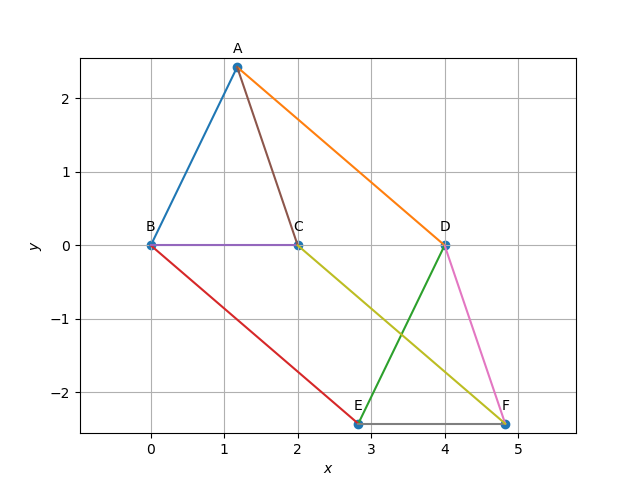
\includegraphics[scale=0.5]{fig.png} 
\caption{Given Figure}
\end{figure}

\section{Solution}
\begin{center}
The input parameters for this construction are
\begin{tabular}{|c|c|}
	\hline
	\textbf{Symbol}&\textbf{Value}\\
	\hline
	r1&2\\
	\hline
	r2&3\\
	\hline
	$\theta$&$\frac{{3}\pi}{10}$\\
	\hline
\end{tabular}
\boldmath
$$\vec{A}=\begin{pmatrix} r1\cos\theta\\ r2\sin\theta\ \end{pmatrix}$$
$$\vec{B}=\begin{pmatrix} 0\\ 0\ \end{pmatrix}$$
$$\vec{D}=\begin{pmatrix} 4\\ 0\ \end{pmatrix}$$
$$\vec{C}={\vec{B}+\vec{D}}/2$$
$$\vec{E}={\vec{B}+\vec{D}-\vec{A}}$$
$$\vec{F}={\vec{E}+\vec{C}-\vec{B}}$$
\unboldmath
\end{center}
\textbf{Direction vectors}

The Direction vectors are
\boldmath
$$\vec{m_1}={\vec{A}-\vec{B}} $$
$$\vec{m_2}={\vec{B}-\vec{C}} $$
$$\vec{m_3}={\vec{C}-\vec{A}} $$
$$\vec{n_1}={\vec{D}-\vec{E}} $$
$$\vec{n_2}={\vec{E}-\vec{F}} $$
$$\vec{n_3}={\vec{F}-\vec{D}} $$
$$\vec{o_1}={\vec{A}-\vec{D}} $$
$$\vec{o_2}={\vec{C}-\vec{F}} $$
\unboldmath
\textbf{To proove\\ i.Quadrilateral ABED is a parallelogram}\\
    Distance between A and B is $\norm{\vec{A-B}}$\\
	Distance between D and E is $\norm{\vec{D-E}}$\\
	if $\norm{\vec{A-B}}$ =  $\norm{\vec{D-E}}$\\
	then AB = DE..........(1)\\
	if $\vec{m_1} \times \vec{n_1}=0$\\
	then AB $\parallel$ DE...........(2)\\
	Because,Two vectors ara parallel when cross product of that two vectors is zero.\\
	From (1) and (2) we can say that ABED is a parallelogram.Because,If one pair of opposite sides of a quadrilateral are equal and parallel to each other,then it is a parallelogram.\\
	$\therefore$ Quadrilateral ABED is a parallelogram.\\ 
\textbf{ii.Quadrilateral BEFC is a parallelogram}\\
    Distance between B and C is $\norm{\vec{B-C}}$\\
	Distance between E and F is $\norm{\vec{E-F}}$\\
	if $\norm{\vec{B-C}}$ =  $\norm{\vec{E-F}}$\\
	then BC = EF..........(3)\\
	if $\vec{m_2} \times \vec{n_2}=0$\\
	then BC $\parallel$ EF...........(4)\\
	Because,Two vectors ara parallel when cross product of that two vectors is zero.\\
	From (3) and (4) we can say that BEFC is a parallelogram.Because,If one pair of opposite sides of a quadrilateral are equal and parallel to each other,then it is a parallelogram.\\
	$\therefore$ Quadrilateral BEFC is a parallelogram.\\ 	
\textbf{iii.AD$\parallel$CF and AD=CF}\\
    Distance between A and D is $\norm{\vec{A-D}}$\\
	Distance between C and F is $\norm{\vec{C-F}}$\\
	if $\norm{\vec{A-D}}$ =  $\norm{\vec{C-F}}$\\
	then AD = CF..........(5)\\
	if $\vec{O_1} \times \vec{O_2}=0$\\
	then AD $\parallel$ CF...........(6)\\
	Because,Two vectors ara parallel when cross product of that two vectors is zero.\\
	From (5) and (6) AD$\parallel$CF and AD=CF \\
\textbf{iv.Quadrilateral ACFD is a parallelogram}\\
   From (iii) we can say that AD$\parallel$CF and AD=CF 
	SO, we can say that ACFD is a parallelogram.Because,If one pair of opposite sides of a quadrilateral are equal and parallel to each other,then it is a parallelogram.\\
	$\therefore$ Quadrilateral ACFD is a parallelogram.\\
\textbf{v.AC=DF}\\
    Distance between A and C is $\norm{\vec{A-C}}$\\
	Distance between D and F is $\norm{\vec{D-F}}$\\
	if $\norm{\vec{A-C}}$ =  $\norm{\vec{D-F}}$\\
	then AC = DF\\
	$\therefore$ AC=DF\\
\textbf{vi.$\Delta ABC \cong \Delta DEF$}  \\
If $\norm{\vec{A-B}}$ =  $\norm{\vec{D-E}}$ and $\norm{\vec{B-C}}$ =  $\norm{\vec{E-F}}$ and $\norm{\vec{A-C}}$ =  $\norm{\vec{D-F}}$\\
Then,$\Delta ABC \cong \Delta DEF$ .Because, If three sides of one triangle are equal to three sides of another triangle, the triangles are congruent.(By SSS Rule)\\
$\therefore$ $\Delta ABC \cong \Delta DEF$

\section{Execution}
*Verify the above proofs in the following code.\\
\framebox{
\url{https://github.com/gowripriya-2002/FWC/blob/main/line_assignment/line.py}}	
\bibliographystyle{ieeetr}
\end{document}

\item 
\iffalse
\documentclass[journal,10pt,twocolumn]{article}
\usepackage[margin=0.5in]{geometry}
\usepackage[cmex10]{amsmath}
\usepackage{array}
\usepackage{booktabs}

% The preceding line is only needed to identify funding in the first footnote. If that is unneeded, please comment it out.
\usepackage{cite}
\usepackage{amsmath,amssymb,amsfonts}
\usepackage{graphicx}
\usepackage{textcomp}
\usepackage{xcolor}
\usepackage{graphicx}
\graphicspath{{./fig}}{}
\def\BibTeX{{\rm B\kern-.05em{\sc i\kern-.025em b}\kern-.08em
    T\kern-.1667em\lower.7ex\hbox{E}\kern-.125emX}}

\usepackage{tikz}
\usetikzlibrary{shapes.geometric}
\usetikzlibrary{shapes.geometric,angles,quotes}


\begin{document}



\newtheorem{theorem}{Theorem}[section]
\newtheorem{problem}{Problem}
\newtheorem{proposition}{Proposition}[section]
\newtheorem{lemma}{Lemma}[section]
\newtheorem{corollary}[theorem]{Corollary}
\newtheorem{example}{Example}[section]
\newtheorem{definition}[problem]{Definition}
%\newtheorem{thm}{Theorem}[section] 
%\newtheorem{defn}[thm]{Definition}
%\newtheorem{algorithm}{Algorithm}[section]
%\newtheorem{cor}{Corollary}
\newcommand{\BEQA}{\begin{eqnarray}}
\newcommand{\EEQA}{\end{eqnarray}}
\newcommand{\define}{\stackrel{\triangle}{=}}
\newcommand*\circled[1]{\tikz[baseline=(char.base)]{
    \node[shape=circle,draw,inner sep=2pt] (char) {#1};}}

\bibliographystyle{article}
%\bibliographystyle{ieeetr}


\providecommand{\mbf}{\mathbf}
\providecommand{\pr}[1]{\ensuremath{\Pr\left(#1\right)}}
\providecommand{\re}[1]{\ensuremath{\text{Re}\left(#1\right)}}
\providecommand{\im}[1]{\ensuremath{\text{Im}\left(#1\right)}}
\providecommand{\qfunc}[1]{\ensuremath{Q\left(#1\right)}}
\providecommand{\sbrak}[1]{\ensuremath{{}\left[#1\right]}}
\providecommand{\lsbrak}[1]{\ensuremath{{}\left[#1\right.}}
\providecommand{\rsbrak}[1]{\ensuremath{{}\left.#1\right]}}
\providecommand{\brak}[1]{\ensuremath{\left(#1\right)}}
\providecommand{\lbrak}[1]{\ensuremath{\left(#1\right.}}
\providecommand{\rbrak}[1]{\ensuremath{\left.#1\right)}}
\providecommand{\cbrak}[1]{\ensuremath{\left\{#1\right\}}}
\providecommand{\lcbrak}[1]{\ensuremath{\left\{#1\right.}}
\providecommand{\rcbrak}[1]{\ensuremath{\left.#1\right\}}}

\newcommand{\sgn}{\mathop{\mathrm{sgn}}}

%\providecommand{\hilbert}{\overset{\mathcal{H}}{ \rightleftharpoons}}
\providecommand{\system}{\overset{\mathcal{H}}{ \longleftrightarrow}}
	%\newcommand{\solution}[2]{\textbf{Solution:}{#1}}
\newcommand{\solution}{\noindent \textbf{Solution: }}
\newcommand{\cosec}{\,\text{cosec}\,}
\providecommand{\dec}[2]{\ensuremath{\overset{#1}{\underset{#2}{\gtrless}}}}
\newcommand{\myvec}[1]{\ensuremath{\begin{pmatrix}#1\end{pmatrix}}}
\newcommand{\mydet}[1]{\ensuremath{\begin{vmatrix}#1\end{vmatrix}}}
	\newcommand*{\permcomb}[4][0mu]{{{}^{#3}\mkern#1#2_{#4}}}
\newcommand*{\perm}[1][-3mu]{\permcomb[#1]{P}}
\newcommand*{\comb}[1][-1mu]{\permcomb[#1]{C}}

%\numberwithin{align}{section}
\numberwithin{align}{subsection}
%\numberwithin{problem}{section}
%\numberwithin{definition}{section}

\let\vec\mathbf




\title{
{Comparision of Angles and Sides of Trapezium\\
Using Matrices and lines}\\

\thanks{Meer Tabres Ali as an intern with FWC IIT Hyderabad. *The author is with the Department of Electrical Engineering, Indian Institute of Technology, Hyderabad 502285 India e-mail: gadepall@iith.ac.in. All content in this manual is released under GNU GPL. Free and open source.}
}
\author{Meer Tabres Ali and G V V Sharma}
\maketitle
\tableofcontents
\section{Problem statement}
\fi
$ABCD$ is trapezium in which $AB \parallel CD$ and $AD=BC$.
Show that, 
\begin{enumerate}
    \item $\angle A = \angle B$
    \item $\angle C = \angle D$
    \item Diagonal $AC$ = Diagonal $BD$
    \item $\triangle ABC  = \triangle BAD$
\end{enumerate}
\iffalse
\solution 
See Fig. 
		\ref{fig:9/8/1/12}.
	\begin{figure}[!h]
		\centering
 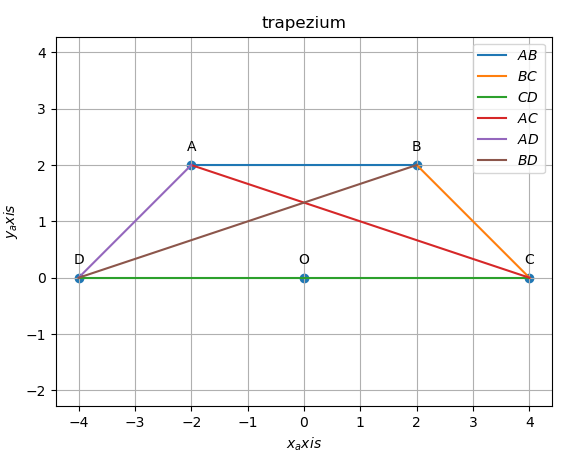
\includegraphics[width=\columnwidth]{chapters/9/8/1/12/figs/trapezium1.png}
		\caption{}
		\label{fig:9/8/1/12}
  	\end{figure}
For $\vec{e}_1$ defined in Appedix \ref{def:matrix-two},
    Let 
\begin{align}
	 \label{eq:9/8/1/12/cang}
		\begin{split}
	\vec{D} &= \vec{0}
	\\
	\vec{C}&= c\vec{e}_1
\\
	\vec{A}&= r\myvec{\cos D \\ \sin D}
\\
	\vec{B}&= \vec{C} +  r\myvec{-\cos C \\ \sin C}
		\end{split}
\end{align}
%
Thus, 
\begin{align}
	 \label{eq:9/8/1/12/cang/a}
	\cos \angle{BAD}
	&= \frac{(\vec{A}-\vec{B})^T(\vec{A}-\vec{D})}{\norm{\vec{A}-\vec{B}}\norm{\vec{A}-\vec{D}}}
	\\
\cos	\angle{CBA}
	 &= \frac{(\vec{B}-\vec{C})^T(\vec{B}-\vec{A})}{\norm{\vec{B}-\vec{C}}\norm{\vec{B}-\vec{A}}}
	 \label{eq:9/8/1/12/cang/b}
%
\end{align}
Substituting from 
	 \eqref{eq:9/8/1/12/cang},
\begin{align}
	 \label{eq:9/8/1/12/cang/abd}
	 (\vec{A}-\vec{B})^T(\vec{A}-\vec{D}) &= r\brak{r\myvec{\cos D+ \cos C  & \sin D - \sin C}-c\vec{e}_1^{\top}}\myvec{\cos D \\ \sin D}
	 \\
	&= r\brak{r\brak{1+ \cos \brak{C+D}  }-c\cos D }
\end{align}
Similarly, 
\begin{align}
	 \label{eq:9/8/1/12/cang/abc}
(\vec{B}-\vec{C})^T(\vec{B}-\vec{A})
	&= r\brak{-r\myvec{\cos D+ \cos C  & \sin D - \sin C}+c\vec{e}_1^{\top}}\myvec{-\cos C \\ \sin C}
	 \\
	&= r\brak{r\brak{1+ \cos \brak{C+D}  }-c\cos D }
\end{align}

	 \eqref{eq:9/8/1/12/cang},
\section{Considerations}
\vspace{0.2cm}
The input parameters are the lengths r, c and angle $\theta$. \\
\vspace{0.2cm}
{


\setlength\extrarowheight{2pt}
\begin{tabular}{|c|c|c|}
	\hline
	\textbf{Symbol}&\textbf{Value}&\textbf{Description}\\
	\hline
	$\vec{O}$ & \myvec{0\\0}
	&Origin\\
	\hline
	r&2.82& Distance of BC, AD\\
	\hline
	c&4&OC\\
	
	\hline
	$\vec{C}$ & \myvec{c \\ 0}

	&Point C on X axes
	\\
\hline
	$\theta$&45 \textdegree &$\angle$BOC\\
	\hline
\end{tabular}
}


\section{Plotting Trapezium}




\vspace{0.25cm}
Plot of Trapezium is shown in figure 1, where point O is origin and points A, B, C and D are the vertices of Trapezium.
\begin{figure}[h]

\caption{trapezium}
\label{fig:trapezium}
\end{figure}


\section{Solution}

\vspace{0.25cm}
\subsection{Finding Co-ordinates O, A, B, C and D}
\begin{flushleft}
Let O be the origin and its coordinates are\\
\vspace{0.25cm}

\center
\vspace{0.4cm}
$\vec{O}$ = \myvec{0\\0}
\endcenter{}
\vspace{0.25cm}
Let C be the point on X-axes and it is expressed as\\
\vspace{0.25cm}
\begin{align}
    \vec{C} = c
    \end{align}

\vspace{0.25cm}
\begin{flushleft}
Let D be the point on Negative X-axes and it will be the image of C,\\
\begin{center}
$\vec{D}$  = -c\\
\end{center}
\vspace{0.2cm}
Therefore, the coordinates of D are\\
\end{flushleft}


\vspace{0.25cm}
\begin{flushleft}
Let r be the distance between point B and C, then\\
\end{flushleft}

\vspace{0.25cm}
$|| \vec{B-C} || $ = r and $|| \vec{A-D} || $ = r\\
\vspace{0.25cm}
\begin{flushleft}
Let $\theta$ be the angle at BOC, then\\
\end{flushleft}
\vspace{0.25cm}
$\angle$BOC = $\theta$\\
\vspace{0.25cm}
\begin{flushleft}
According to the vector geometry formulaes, the vector B can be expresssed as\\
\end{flushleft}
\vspace{0.25cm}
\begin{align}
   \vec{B}= r \myvec{cos\theta \\ sin\theta}
\end{align}

\vspace{0.35cm}
\begin{flushleft}
From ABCD trapezium, \\
\end{flushleft}
\begin{center}
$\vec{A} =\vec{B}-  \vec{C}$\\
\end{center}

\center
\vspace{0.4cm}
= \myvec{rcos $$\theta$$ \\ rsin $$\theta$$} - \myvec{c \\ 0}
   
\endcenter{}
		= \myvec{-c+rcos $$ \theta$$ \\ rsin$$\theta$$}
	\\
\vspace{0.3cm}
\begin{flushleft}
From triangle ODA,
$\boldsymbol{OD+DA=OA}$, \\
\vspace{0.2cm} 
$\implies$ -c+rcos$\theta$ = -r cos $\theta$\\
\end{flushleft}
\vspace{0.35cm}
	= \myvec{-rcos $$ \theta$$ \\ rsin$$\theta$$} \\
\endcenter{}
	$\implies$ $\vec{A}$
	= r\myvec{-cos $$ \theta$$ \\ sin$$\theta$$} \\

Let c=4, r=2.82 and $\theta$=45 \textdegree \\

Then all the four coordinates will be, \\

\vspace{0.3cm}
$\vec{O}$=\myvec{0 \\ 0}, $\vec{A}$=\myvec{-2 \\ 2}, $\vec{B}$=\myvec{2 \\ 2}, $\vec{C}$=\myvec{4 \\ 0}, $\vec{D}$=\myvec{-4 \\ 0}
\\

\subsection{Calculation of Angles A and B}
\vspace{0.25cm}
To find angle $\angle$A:\\

\begin{center}
    

$\vec{A-D}$ = \myvec{-2 \\ 2} - \myvec{-4 \\ 0}
	= \myvec{2 \\ 2}

\begin{flushleft}
and \\
\end{flushleft}


$\vec{A-B}$ = \myvec{-2 \\ 2} -\myvec{2 \\ 2} = \myvec{-4 \\ 0}
	\\

\end{center}
\vspace{0.4cm}
\begin{align}
\angle BAD = arccos \vec{\frac{(A-D).(A-B)}{||A-D ||. ||A-B||}}
\end{align}
\vspace{0.4cm}
\begin{align}
\angle BAD = arccos \frac{(2 \hspace{0.32cm}  2)^T . (-4 \hspace{0.25cm}   0) } {\sqrt{2^2+2^2}.\sqrt{4^2+0}}
\end{align}

\begin{align}
= arccos \frac{-8 } {\sqrt{8}.\sqrt{16}} = arccos (-0.707) 
\end{align}
\begin{flushleft}
$\implies$   $\angle$ BAD = 135 \textdegree\\
\vspace{0.3cm}
$\implies$   $\angle$ A = 135 \textdegree
\end{flushleft}

\vspace{0.5cm}
\begin{flushleft}
To find angle $\angle$ B: \\
\end{flushleft}

\vspace{0.35cm}
$\vec{B-A}$ = \myvec{2 \\ 2}-\myvec{-2 \\ 2}
	= \myvec{4\\0}
and \\

$\vec{B-C}$ = \myvec{2 \\ 2} -\myvec{4\\0} = \myvec{-2 \\2} 
\vspace{0.25cm}	
\begin{align}
\angle BAD = arccos \vec {\frac{(A-D).(A-B)}{||A-D||.||A-B||}}
\end{align}

\begin{align}
\angle BAD = arccos \frac{(4, 0)^T .(-2, 2)}{\sqrt{4^2}.\sqrt{2^2+2^2} }
\end{align}

\begin{align}
= arccos \frac{-8 } {\sqrt{16}.\sqrt{8}} =arccos (-0.707)
\end{align}

\begin{flushleft}
$\implies$   $\angle$ ABC = 135 \textdegree\\
\vspace{0.3cm}
$\implies$   $\angle$ B = 135 \textdegree
\\
\vspace{0.3cm}
Therefore $\angle A$ = $\angle B$
\end{flushleft}

\subsection{Calculation of Angles C and D}
\vspace{0.25cm}

To find angle $\angle$C:\\
$\vec{C-O}$ = \myvec{4\\0} - \myvec{0\\0}
	= \myvec{4\\0}
and 

$\vec{C-B}$ = \myvec{4\\0}- \myvec{2\\2} = \myvec{2\\-2}
\\

\begin{align}
\angle OCB = arccos \vec{\frac{(C-O).(C-B)}{||C-O ||. ||C-B||}}
\end{align}

\begin{align}
\angle BAD = arccos \frac{(4 \hspace{0.15cm} 0)^T . (2 \hspace{0.15cm} -2) } {\sqrt{4^2}.\sqrt{2^2+2^2}}
\end{align}

\begin{align}
= arccos \frac{8 } {\sqrt{16}.\sqrt{8}} = arccos (0.707)
\end{align}
\begin{flushleft}
$\implies$   $\angle$ OCB = 45 \textdegree\\
\vspace{0.3cm}
$\implies$   $\angle$ C = 45 \textdegree
\end{flushleft}

\vspace{0.5cm}
\begin{flushleft}
To find angle $\angle$ D: \\
\end{flushleft}
\vspace{0.2cm}
\center
$\vec{D-O}$ = \myvec{-4\\0}-\myvec{0\\0}= \myvec{-4 \\ 0}
\\
\endcenter
\begin{flushleft}
and \\
\end{flushleft}


$\vec{D-A}$ = \myvec{-4 \\ 0} -\myvec{-2 \\ 2} = \myvec{-2 \\ -2}

\endcenter

\begin{align}
\angle ODB = arccos \vec{\frac{(D-O).(D-B)}{||D-O ||. ||D-B||}}
\end{align}

\begin{align}
\angle ODB = arccos \frac{(-4 \hspace{0.29cm} 0)^T .(-2 \hspace{0.22cm} -2)}{\sqrt{4^2}.\sqrt{2^2+2^2} }
\end{align}

\begin{align}
= arccos \frac{8} {\sqrt{8}.\sqrt{16}} = arccos (0.707)
\end{align}

\begin{flushleft}
$\implies$   $\angle$ ODB = 45 \textdegree\\
\vspace{0.3cm}
$\implies$   $\angle$ D = 45 \textdegree
\end{flushleft}

Therefore $\angle C$ = $\angle D$

\subsection{Calculation of Diagonals AC and BD}
\vspace{0.2cm}
\begin{flushleft}
Calculation of Diagonal AC:\\
\end{flushleft}

\vspace{0.1cm}

$\vec{A-C}$ = \myvec{-2 \\ 2} - \myvec{4 \\ 0} = \myvec{-6\\2}
	\\
\begin{flushleft}
Legth of Diagonal AC,\\
\end{flushleft}


$\vec{||A-C||}$ = $ || \myvec{-6 \\ 2} ||$
	\\
\vspace{0.25cm}
= $\sqrt{(-6)^2+2^2}$ = 6.32\\
\vspace{0.3cm}
$\implies$ $\vec{||A-C||}$=6.32\\

\vspace{0.3cm}
\begin{flushleft}
Calculation of Diagonal BD:\\
\end{flushleft}

\vspace{0.25cm}

$\vec{B-D}$ = \myvec{2\\2}- \myvec{-4\\0} = \myvec{6 \\ 2}
	\\
\begin{flushleft}
Length of Diagonal BD,\\
\end{flushleft}

$\vec{||B-D||}$ =  $||\myvec{6 \\2}||$
	\\
\vspace{0.25cm}
= $\sqrt{6^2+2^2}$ = 6.32\\
\vspace{0.25cm}
$\implies$ $\vec{||B-D||}$=6.32\\
\begin{flushleft}
Therefore both diagonals are equal,  AC = BD \\
\end{flushleft}

\subsection{Comparing $\triangle$ ABC and $\triangle$ BAD }
\begin{flushleft}
\vspace{0.25cm}
For Triangle ABC:\\
\vspace{0.25cm}
$\angle ABC = \angle AOC = \pi -\theta$ = 135 \textdegree \\
\vspace{0.25cm}
and\\
\vspace{0.25cm}
Base =Diagonal AC  = $\vec{||A-C||}$ = 6.32\\
\vspace{0.35cm}

For Triangle BAD:\\
\vspace{0.25cm}
$\angle BAD = \angle BOD = \pi -\theta$ = 135 \textdegree \\
\vspace{0.25cm}
and\\
\vspace{0.25cm}
Base =Diagonal AC  = $\vec{||B-D||} $ = 6.32\\
\vspace{0.35cm}
As base and opposite angles are same, both triangles are symmetrical.
\vspace{0.25cm}\\
Therefore  $\triangle$ ABC and $\triangle$ BAD
\end{flushleft}

\section{Software}
\centering
Download the codes given in the link below and execute them.\\
\begin{table}[h]
\centering
\begin{tabular}{|c|} \hline
\rule{0pt}{10pt} 
https://github.com/meertabresali-FWC-IITH/project/blob \\
/main/Asgn4.matrixline/line.py\\
\\\hline
 \end{tabular}
\end{table}
\section{Conclusion}
\begin{flushleft}
In this program, the following points have been verified.\\
\vspace{0.1cm}
\begin{enumerate}
    \item $\angle$ A = $\angle$ B\\
    \item $\angle$ C = $\angle$ D\\
    \item Diagonal AC = Diagonal BD\\
    \item $\triangle$ ABC  = $\triangle$ BAD \\
\end{enumerate}
\end{flushleft}
\end{document}
\fi






\end{enumerate}

%\section{Mid Point Theorem}
%\begin{enumerate}
\item 
\label{chapters/9/8/2/1}
\iffalse
\documentclass[journal,10pt,twocolumn]{article}
\usepackage{graphicx}
\usepackage[margin=0.5in]{geometry}
\usepackage[cmex10]{amsmath}
\usepackage{array}
\usepackage{booktabs}
\usepackage{listings}
\title{\textbf{Line Assignment}}
\author{Bhavani Kanike}
\date{October 2022}

\providecommand{\norm}[1]{\left\lVert#1\right\rVert}
\providecommand{\abs}[1]{\left\vert#1\right\vert}
\let\vec\mathbf
\newcommand{\myvec}[1]{\ensuremath{\begin{pmatrix}#1\end{pmatrix}}}
\newcommand{\mydet}[1]{\ensuremath{\begin{vmatrix}#1\end{vmatrix}}}
\providecommand{\brak}[1]{\ensuremath{\left(#1\right)}}

\begin{document}

\maketitle
\paragraph{\textit{Problem Statement} 
\fi
ABCD is a quadrilateral in which $\vec{P}, \vec{Q}, \vec{R}$ and $\vec{S}$ are mid-points of the sides AB, BC, CD and DA (see Fig \ref{fig:9/8/2/1}). AC is a diagonal. 
		
Show that 
\begin{enumerate}
	\item $SR \parallel AC$ and $SR =\frac{1}{2} AC$
\item $PQ = SR$
\item $PQRS$ is a parallelogram.
\end{enumerate}
 	\begin{figure}
		\centering
 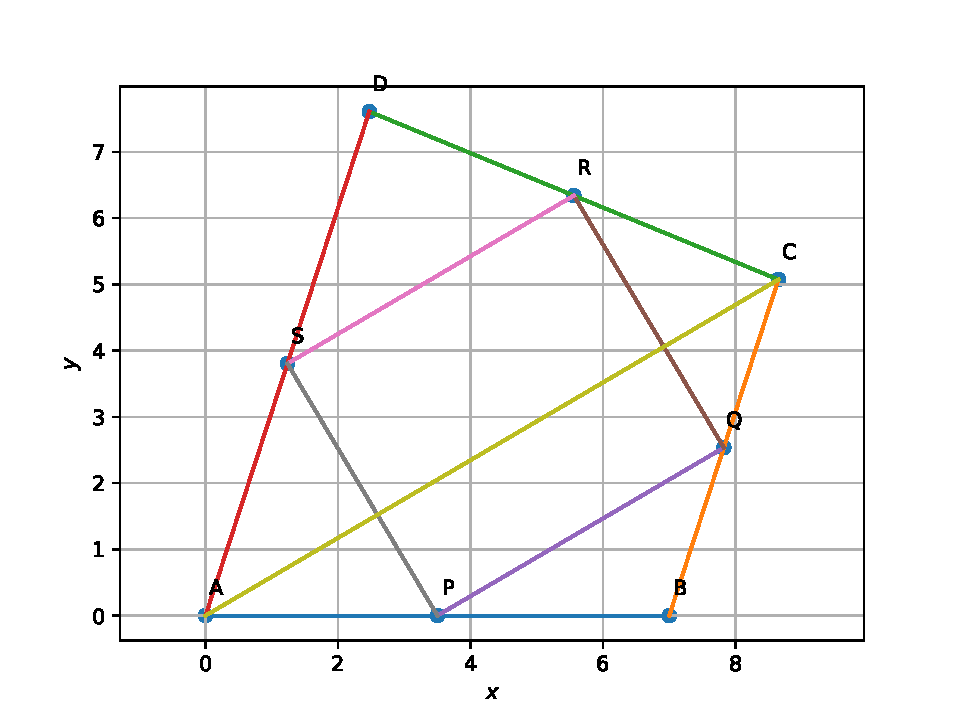
\includegraphics[width=\columnwidth]{chapters/9/8/2/1/figs/line1.pdf}
		\caption{}
		\label{fig:9/8/2/1}
  	\end{figure}
	\solution 
	Using 
	  \eqref{eq:section_formula},
	\begin{align}
		\label{eq:9/8/2/1}
		\begin{split}
		\vec{P} &= \frac{\vec{A}+\vec{B}}{2}\\
 \vec{Q} &= \frac{\vec{C}+\vec{B}}{2}\\
 \vec{R} &= \frac{\vec{C}+\vec{D}}{2}\\
 \vec{S} &= \frac{\vec{D}+\vec{A}}{2}
		\end{split}
	\end{align}
\begin{enumerate}
	\item
	Consequently, 
	\begin{align}
\vec{R}
		-\vec{S} &= \frac{\vec{C}-\vec{A}}{2}
		\\
		\implies SR &\parallel AC
	\end{align}
	Also, 
	\begin{align}
		\norm{\vec{R}
		-\vec{S}} &= \frac{\norm{\vec{C}-\vec{A}}}{2}
		\\
		\implies SR &= \frac{1}{2}AC
	\end{align}
\item 	From 
		\eqref{eq:9/8/2/1},
	\begin{align}
\vec{R}
		-\vec{S} = \vec{Q}-\vec{P}
	\end{align}
	which means that $PQRS$ is a parallelogram and $PQ = SR$.
\end{enumerate}
%
\iffalse
\begin{figure}[h]
\centering
\includegraphics[width=1\columnwidth]
\caption{Figure}
\label{fig:triangle}
\end{figure}

\section*{Solution}

$\boldsymbol Given :$  ABCD is a Quadrilateral P,Q,R and S are the midpoints of line AB,BC,CD,DA.We can obtain the points P,Q,R and S from A,B,C and D and are given by\\\\
\boldmath
\unboldmath
(3) To prove that PQRS is a parallelogram we need to prove  PQ // SR
To prove SR $\parallel$ PQ\\
Direction vector of line SR  $\boldsymbol {(R-S) =  \frac{(C-A)}{2}}$\\\\
Direction vector of line PQ  $\boldsymbol {(Q-P)= \frac{(C-A)}{2}}$\\\\
\begin{equation}
	\boldsymbol {(R-S) = (Q-P) = \frac{(C-A)}{2}}\\
\end{equation}
Since the direction vectors of line SR and PQ are in same direction\\\\
$SR \parallel PQ$\\
Therefore,
$\boldsymbol{ PQRS }$ is a parallelogram\\\\

	
(1)  Directional vector of line SR  = $\boldsymbol {(R-S)}$ = $\frac{\boldsymbol{(C-A)}}{2} $\\
Directional vector of line AC  = $\boldsymbol {(C-A)}$\\

It is observed that the constant k is $\frac{1}{2}$

Therefore
\begin{equation}
	SR \parallel AC
\end{equation} 

and from equation 1 
\begin{equation}
	\boldsymbol {SR = \frac{1}{2}AC}    
\end{equation}\\


(2)   To prove PQ = SR\\ 
		From euqation 1\\\\
\begin{equation}
		\boldsymbol{ (Q-P) = (R-S) = \frac{(C-A)}{2}}
\end{equation}
	 



\section{Execution}
The below python code realizes the construction:
\begin{lstlisting}
https://github.com/bhavani360/FWC_assignments
\end{lstlisting}
	
\section*{Construction}
The dimensions of the Quadrilateral ABCD are taken as below\\
{
\setlength\extrarowheight{2pt}
\centering
	\begin{tabular}{|c|c|}
	\hline
	\textbf{symbol}&\textbf{value}\\
	\hline
	r&8\\
	\hline
	$\theta$&pi/2.5\\
	\hline
	d&7\\
	\hline
	A&(0,0)\\
	\hline
	B&(d,0)\\
	\hline
	D&(rcos$\theta$,rsin$\theta$)\\
	\hline
	C&(D/1.5)+B\\
	\hline
\end{tabular}
}
\end{document}
\fi


\item 
\item 
\iffalse
\documentclass[journal,10pt,twocolumn]{article}
\usepackage{graphicx}
\usepackage[margin=0.5in]{geometry}
\usepackage{amsmath}
\usepackage{array}
\usepackage{booktabs}
\usepackage{amssymb}
\title{\textbf{Matrix Assignment}}
\author{lakshmi kamakshi}
\date{September 2022}

\begin{document}

\maketitle
\fi
$ABCD$ is a rectangle and $\vec{P}, \vec{Q}, \vec{R}$ and $\vec{S}$ are mid-points of the sides $AB, BC, CD$ and $DA
$ respectively. Show that the quadrilateral $PQRS$ is a rhombus.
 	\begin{figure}
		\centering
 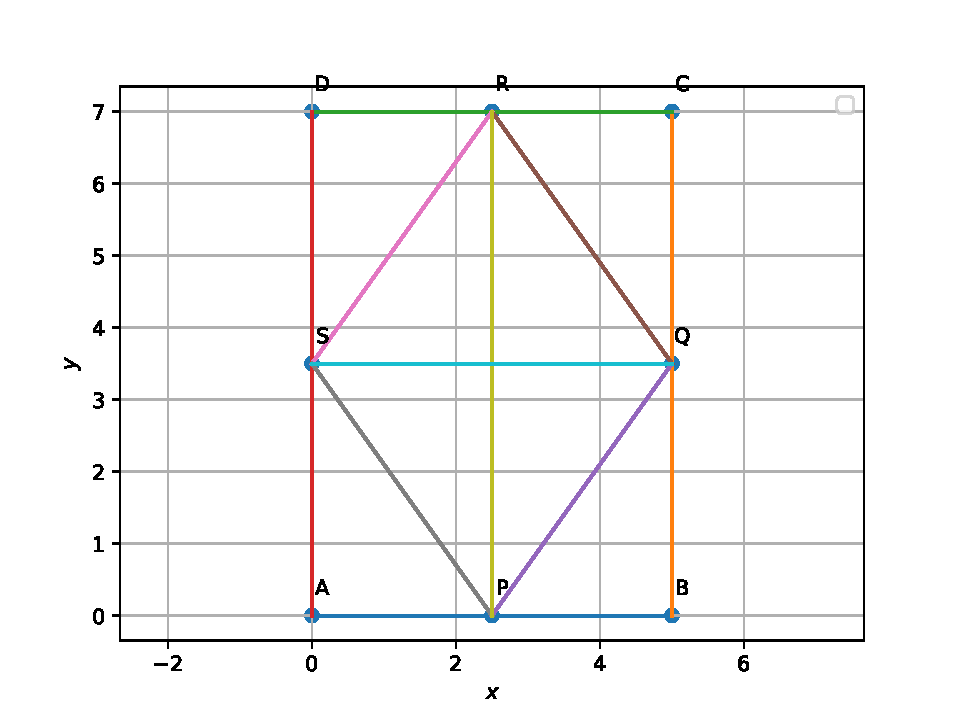
\includegraphics[width=\columnwidth]{chapters/9/8/2/3/figs/fig.pdf}
		\caption{}
		\label{fig:9/8/2/3}
  	\end{figure}
	\\
	\solution From 
Problem \ref{chapters/9/8/2/1}, it is obvious that $PQRS$ is a parallelogram.  Further, 
from 
		\eqref{eq:9/8/2/1},
	\begin{align}
		\brak{\vec{P}
		-\vec{R}}^{\top} \brak{ \vec{S}-\vec{Q}} &= 
		 \brak{\vec{A}+\vec{B}- \vec{C}-\vec{D}}^{\top}
		 \brak{\vec{A}+\vec{D}- \vec{B}-\vec{C}}
		 \\
		 &= \vec{0}
	\end{align}
	since 
	\begin{align}
		\brak{\vec{A}
		-\vec{D}}^{\top} \brak{ \vec{A}-\vec{B}} &= \vec{0}
		\\
		\norm{ \vec{A}-\vec{D}} &= 
\norm{ \vec{A}-\vec{B}}
	\end{align}
	as $ABCD$ is a rectangle.  Thus, the diagonals $PR$ and $SQ$ bisect each other proving that $PQRS$ is a rhombus.
\iffalse
\vspace{5mm}

\section*{Solution}

Using triangle law of vector addition:
\begin{equation}
	\overline{PQ}= \overline{PB} + \overline{BQ} 
\end{equation}
\begin{equation}
		  \overline{PQ}  = \frac{1}{2}\overline{AB} + \frac{1}{2}\overline{BC} \\
\end{equation}
\begin{equation}
	\overline{PQ} =\frac{1}{2}(\overline{AB+BC})\\
\end{equation}
\begin{equation}
	  \overline{PQ} =\frac{1}{2}\overline{AC} \\
\end{equation}

Similarily,using triangle law of vector addition:
\begin{equation}
	\overline{PS}= \overline{PA} + \overline{AS} 
\end{equation}
\begin{equation}
		  \overline{PS}  = \frac{1}{2}\overline{BA} + \frac{1}{2}\overline{AD} \\
\end{equation}
\begin{equation}
	\overline{PS} =\frac{1}{2}(\overline{BA+AD})\\
\end{equation}
\begin{equation}
	  \overline{PS} =\frac{1}{2}\overline{BD} \\
\end{equation}
\\ABCD is a rectangle and has the following properties:
\begin{enumerate}
	\item Opposite sides are equal
\item All angles are equal
\item lengths of diagonals are equal
\item Diagonals are perpendicular to each other.
\end{enumerate}
	\begin{equation}
AC = BD 
	\end{equation}
	\begin{equation}
		AC \perp BD
	\end{equation}
	\begin{equation}
		\boldsymbol{PQ} = \boldsymbol{PS}
	\end{equation}
\\ similarly, the vector equations of QR,SR can be derived as:
\begin{equation}
	\overline{QR}= \overline{QC} + \overline{CR} 
\end{equation}
	
\begin{equation}
		  \overline{QR}  = \frac{1}{2}\overline{BC} + \frac{1}{2}\overline{CD} \\
\end{equation}
\begin{equation}
	\overline{PQ} =\frac{1}{2}(\overline{BC+CD})\\
\end{equation}
\begin{equation}
	  \overline{PQ} =\frac{1}{2}\overline{BD} \\
\end{equation}


\begin{equation}
	\overline{SR}= \overline{SD} + \overline{DR} 
\end{equation}
\begin{equation}
		  \overline{SR}  = \frac{1}{2}\overline{AD} + \frac{1}{2}\overline{DC} \\
\end{equation}
\begin{equation}
	\overline{SR} = \frac{1}{2}(\overline{AD}+\overline{DC})
\end{equation}
\begin{equation}
	\overline{SR} = \frac{1}{2}\overline{AC}
\end{equation}
from the equations (),():
\begin{equation}
	SR = QS
\end{equation}
\\ Thus, all sides of the quadrilateral PQRS are equal
\\ The diagonals of the Quadrilateral PQRS are given by:
\begin{equation}
	PR = PS+PQ
	\because
\end{equation}
parallelogram law of addition
\begin{equation}
	QS = PS-PQ
	\because
\end{equation}
triangle law of addition
\\ \begin{equation}
	PR = \frac{1}{2}\overline{AC}+\frac{1}{2}\overline{BD}
\end{equation}
\\ \begin{equation}
        QS = \frac{1}{2}\overline{AC}-\frac{1}{2}\overline{BD}
\end{equation}
\\ For a quadrilateral to be rhombus the diagonals should perpendicularly bisect each other
\begin{equation}
	PR.QS = \frac{1}{4}((\overline{AC}+\overline{BD})(\overline{AC}-\overline{BD}))
\end{equation}
\begin{equation}
	PR.QS = 0
\end{equation}
\\Since the dot product of the diagonals is 0, the diagonals are perpendicular
\section*{Construction}
Since , all sides of the qudarilateral PQRS are equal and the digonals are perpendicular to each other, the Quadrilateral is a Rhombus



\section*{Construction}
The dimensions of the rectangle are taken as below\\
{
\setlength\extrarowheight{2pt}
\centering
	\begin{tabular}{|c|c|}
	\hline
	\textbf{vertex}&\textbf{co-ordinates}\\
	\hline
	A&(0,0)\\
	\hline
	B&(5,0)\\
	\hline
	C&(5,7)\\
	\hline
	D&(0,7)\\
	\hline
\end{tabular}
}
\end{document}
\fi

\item 
\item 
\iffalse
\def\mytitle{PARALLELOGRAM}
\def\myauthor{Soundarya Naru}
\def\contact{narusoundarya2002@gmail.com}
\def\mymodule{Future Wireless Communication (FWC)}
\documentclass[10pt, a4paper]{article}
\usepackage[a4paper,outer=1.5cm,inner=1.5cm,top=1.75cm,bottom=1.5cm]{geometry}
\twocolumn
\usepackage{setspace}
\doublespacing
\usepackage{graphicx}
\graphicspath{{./images/}}
\usepackage[colorlinks,linkcolor={black},citecolor={blue!80!black},urlcolor={blue!80!black}]{hyperref}
\usepackage[parfill]{parskip}
\usepackage{lmodern}
\usepackage{tikz}
	\usepackage{physics}
%\documentclass[tikz, border=2mm]{standalone}
\usepackage{karnaugh-map}
%\documentclass{article}
\usepackage{tabularx}
\usepackage{circuitikz}
\usetikzlibrary{calc}
\usepackage{amsmath}
\usepackage{amssymb}
\usepackage{physics}
\renewcommand*\familydefault{\sfdefault}
\usepackage{watermark}
\usepackage{lipsum}
\usepackage{xcolor}
\usepackage{listings}
\usepackage{float}
\usepackage{titlesec}
\providecommand{\mtx}[1]{\mathbf{#1}}
\titlespacing{\subsection}{1pt}{\parskip}{3pt}
\titlespacing{\subsubsection}{0pt}{\parskip}{-\parskip}
\titlespacing{\paragraph}{0pt}{\parskip}{\parskip}
\newcommand{\figuremacro}[5]{
    \begin{figure}[#1]
        \centering
        \includegraphics[width=#5\columnwidth]{#2}
        \caption[#3]{\textbf{#3}#4}
        \label{fig:#2}
    \end{figure}
}
\newcommand{\myvec}[1]{\ensuremath{\begin{pmatrix}#1\end{pmatrix}}}
\let\vec\mathbf
\lstset{
frame=single, 
breaklines=true,
columns=fullflexible
}

%\thiswatermark{\centering \put(181,-119.0){\includegraphics[scale=0.13]{IIT_logo.png}} }
\title{\mytitle}
\author{\myauthor\hspace{1em}\\\contact\\FWC22012\hspace{6.5em}IITH\hspace{0.5em}\mymodule\hspace{6em}ASSIGN-5}
\date{}
\begin{document}
	\maketitle
	\tableofcontents
   \section{Problem}
   \fi
 In a parallelogram ABCD, $\vec{E}$ and $\vec{F}$ are the
mid-points of sides AB and CD respectively
(see Fig. 
		\ref{fig:9/8/2/5})
Show that the line segments AF
and EC trisect the diagonal BD.

 	\begin{figure}
		\centering
 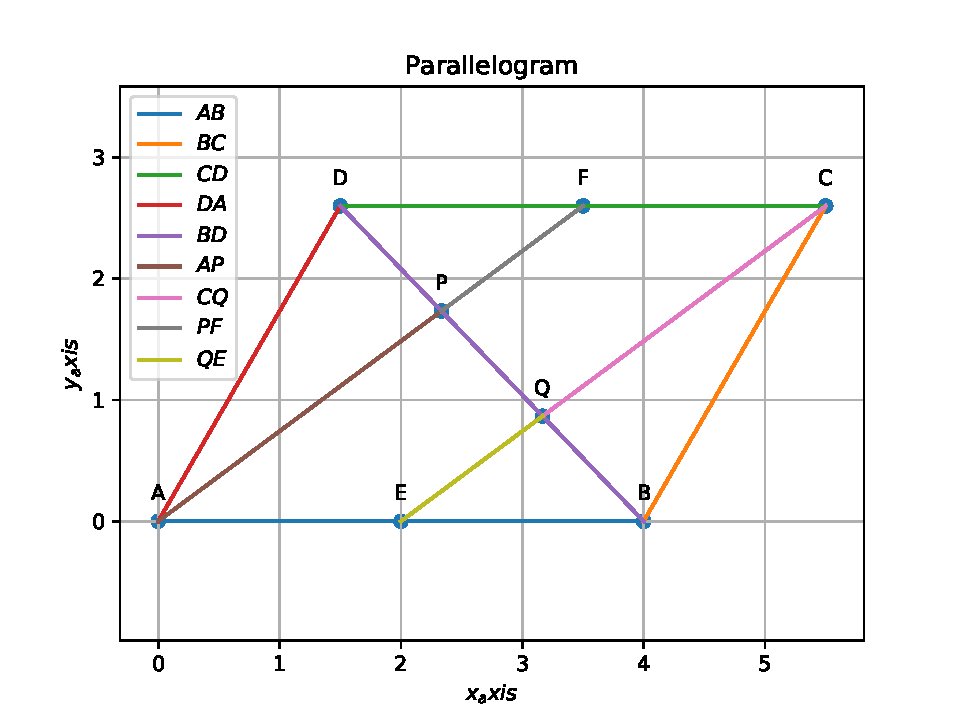
\includegraphics[width=\columnwidth]{chapters/9/8/2/5/figs/line_1.pdf}
		\caption{}
		\label{fig:9/8/2/5}
  	\end{figure}

	\iffalse

	   % 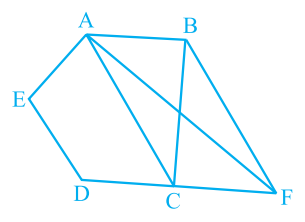
\includegraphics[scale=BB1.0]{diag_1.png}
\begin{center}
   \section{Solution1}

The input parameters for this construction are 
\begin{center}
\begin{tabular}{|c|c|}
	\hline
	\textbf{Symbol}&\textbf{Value}\\
	\hline
	b&6\\
	\hline
	r&5\\
	\hline
	$\theta$&$\frac{\pi}{3}$\\
	\hline
\end{tabular}
\begin{center}
$\vec{A}=\myvec{0\\0}$\\
$\vec{D}=\myvec{r\cos\theta \\ r\sin\theta}$\\
$\vec{B}=\myvec{0\\b}$\\
$\vec{C} = \vec{B}+\vec{C}$\\
\fi
\begin{proof}
From the given information,
	\begin{align}
		\vec{E}=\frac{\vec{A}+\vec{B}}{2}\\
\vec{F}=\frac{\vec{C}+\vec{D}}{2}
	\end{align}
	Hence, 
	\begin{align}
		\vec{E}-\vec{C}&=\frac{\vec{A}-\vec{C}+\vec{B}-\vec{C}}{2}\\
		\vec{A}-\vec{F}&=\frac{\vec{A}-\vec{C}+\vec{A}-\vec{D}}{2}
	\end{align}
	Since $ABCD$ is a parallelogram,
	\begin{align}
		\vec{B}-\vec{C} &= 
	\vec{A}-\vec{D}
	\\
	\implies 
		\vec{E}-\vec{C} &=
\vec{A}-\vec{F}
	\end{align}
	Thus, $AF \parallel EC$.  From Appendix
	  \ref{prop:two-tri-bpt-conv},  using the fact that $\vec{F}$ is the mid point of $CD$, we conclude that $\vec{P}$ is the mid point of $DQ$.  Similarly, it can be shown that $\vec{Q}$ is the mid point of $BP$.
\end{proof}
\iffalse
\end{center}
\end{center}
\textbf{To Prove:} PQ=QB=DP
		\begin{center}
		$\vec{P}=(\vec{2D}+\vec{B})/3$\\
$\vec{Q}=(\vec{2B}+\vec{D})/3$\\
		The distance between P and Q is $\norm{\vec{P}-\vec{Q}}$\\
		The distance between Q and B is $\norm{\vec{Q}-\vec{B}}$\\
		The distance between D and P is $\norm{\vec{D}-\vec{P}}$\\
		if $\norm{\vec{P}-\vec{Q}}$=$\norm{\vec{Q}-\vec{B}}$=$\norm{\vec{D}-\vec{P}}$\\
		then PQ=QB=DP..........(1)\\
		From equation (1) we can say that\\
		 The line segments AF and EC trisect the diagonal BD.\\
		\end{center}
		\section{Solution2}
	 In $\Delta DQC$\\
	 \begin{center}
      F is midpoint of line DC\\
      \end{center}
      \begin{equation}
        	\vec{F}=(\vec{D}+\vec{C})/2
      \end{equation}
       \begin{center}
% $\boldsymbol{FP} \parallel \boldsymbol{QC}$\\
	By converting midpoint theorem \\
	P is mid point of line DQ\\
	\begin{equation}
			\vec{P}=(\vec{D}+\vec{Q})/2
	\end{equation}
			then,\\
			\end{center}
			\begin{center}
			The distance between D and P is $\norm{\vec{D}-\vec{P}}$ \\
			The distance between P and Q is $\norm{\vec{P}-\vec{Q}}$\\
			if $\norm{\vec{D}-\vec{P}}$=$\norm{\vec{P}-\vec{Q}}$ \\
			\end{center}
			\begin{equation}
                DP=PQ 
			\end{equation}
			\begin{center}
			%$\therefore$ AF and EC bisect BD\\
\end{center}						 
	In $\Delta APB$\\
	\begin{center}
	E is midpoint of line AB\\
	\begin{equation}
			\vec{E}=(\vec{A}+\vec{B})/2
			\end{equation}
		  %$\boldsymbol{EQ}\parallel \boldsymbol{AP}$\\
	By converting of mid point theorem\\
		Q is midpoint of BP\\
		\begin{equation}
			\vec{Q}=(\vec{B}+\vec{P})/2
			\end{equation}
			then,\\
	\end{center}
	\begin{center}
	The distance between P and Q is $\norm{\vec{P}-\vec{Q}}$\\
	The distance between Q and B is $\norm{\vec{Q}-\vec{B}}$\\
	if $\norm{\vec{P}-\vec{Q}}$=$\norm{\vec{Q}-\vec{B}}$\\
	\end{center}
	\begin{equation}
	PQ=QB
	\end{equation}
	\begin{center}
	$\norm{\vec{D}-\vec{P}}$=$\norm{\vec{P}-\vec{Q}}$=$\norm{\vec{Q}-\vec{B}}$\\
$\therefore$ from (5),(8) \\
\begin{equation}
DP=PQ=QB
\end{equation}	
		from equation (9) we can say that the \\	
	 The line segments AF and EC trisect the diagonal BD.\\
	 AF and EC trisect BD.
	\end{center}
The below python code realizes the above construction:	\\
\begin{lstlisting}
https://github.com/soundaryanaru/FWC-assignments/tree/main/Matrix/Line_assignment/code
\end{lstlisting}
 
\section{Construction}
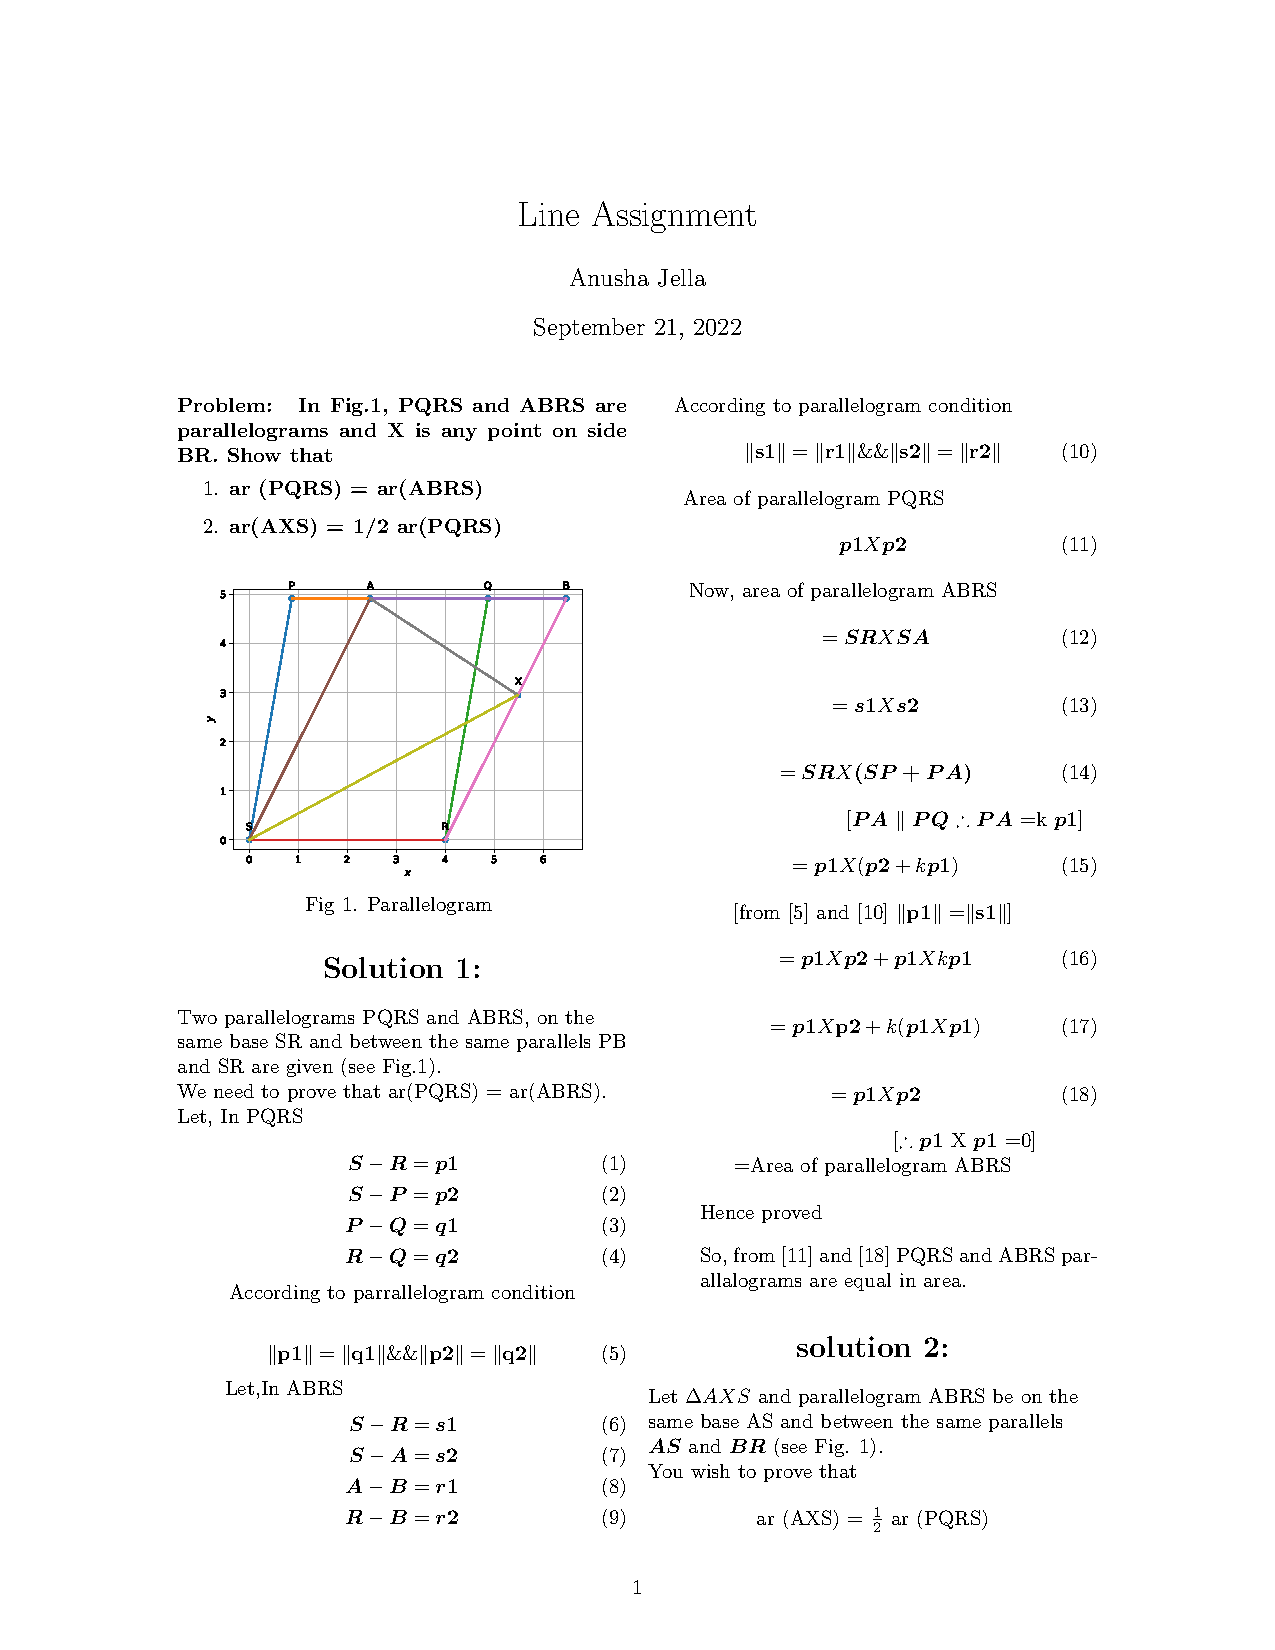
\includegraphics[scale=0.7]{line_1.pdf}
 	
\bibliographystyle{ieeetr}
\end{document}
\fi

\item 
%\iffalse
\documentclass[journal,12pt,twocolumn]{IEEEtran}

\usepackage[utf8]{inputenc}
\usepackage{kvmap}
\usepackage{graphics} 

\usepackage{setspace}
\usepackage{gensymb}

\singlespacing

\usepackage{amsthm}

\usepackage{mathrsfs}
\usepackage{txfonts}
\usepackage{stfloats}
\usepackage{bm}
\usepackage{cite}
\usepackage{cases}
\usepackage{subfig}

\usepackage{longtable}
\usepackage{multirow}

\usepackage{enumitem}
\usepackage{mathtools}
\usepackage{steinmetz}
\usepackage{tikz}
\usepackage{circuitikz}
\usepackage{verbatim}
\usepackage{tfrupee}
\usepackage[breaklinks=true]{hyperref}
\usepackage{graphicx}
\usepackage{tkz-euclide}
\usepackage{float}

\usetikzlibrary{calc,math}
\usepackage{listings}
    \usepackage{color}                                            %%
    \usepackage{array}                                            %%
    \usepackage{longtable}                                        %%
    \usepackage{calc}                                             %%
    \usepackage{multirow}                                         %%
    \usepackage{hhline}                                           %%
    \usepackage{ifthen}                                           %%
    \usepackage{lscape}     
\usepackage{multicol}
\usepackage{chngcntr}

\DeclareMathOperator*{\Res}{Res}

\renewcommand\thesection{\arabic{section}}
\renewcommand\thesubsection{\thesection.\arabic{subsection}}
\renewcommand\thesubsubsection{\thesubsection.\arabic{subsubsection}}

\renewcommand\thesectiondis{\arabic{section}}
\renewcommand\thesubsectiondis{\thesectiondis.\arabic{subsection}}
\renewcommand\thesubsubsectiondis{\thesubsectiondis.\arabic{subsubsection}}

\hyphenation{op-tical net-works semi-conduc-tor}
\def\inputGnumericTable{}                                 %%

\lstset{
%language=C,
frame=single, 
breaklines=true,
columns=fullflexible
}
\begin{document}

\newtheorem{theorem}{Theorem}[section]
\newtheorem{problem}{Problem}
\newtheorem{proposition}{Proposition}[section]
\newtheorem{lemma}{Lemma}[section]
\newtheorem{corollary}[theorem]{Corollary}
\newtheorem{example}{Example}[section]
\newtheorem{definition}[problem]{Definition}

\newcommand{\BEQA}{\begin{eqnarray}}
\newcommand{\EEQA}{\end{eqnarray}}
\newcommand{\define}{\stackrel{\triangle}{=}}
\newcommand\hlight[1]{\tikz[overlay, remember picture,baseline=-\the\dimexpr\fontdimen22\textfont2\relax]\node[rectangle,fill=blue!50,rounded corners,fill opacity = 0.2,draw,thick,text opacity =1] {$#1$};}
\bibliographystyle{IEEEtran}
\providecommand{\mbf}{\mathbf}
\providecommand{\pr}[1]{\ensuremath{\Pr\left(#1\right)}}
\providecommand{\qfunc}[1]{\ensuremath{Q\left(#1\right)}}
\providecommand{\sbrak}[1]{\ensuremath{{}\left[#1\right]}}
\providecommand{\lsbrak}[1]{\ensuremath{{}\left[#1\right.}}
\providecommand{\rsbrak}[1]{\ensuremath{{}\left.#1\right]}}
\providecommand{\brak}[1]{\ensuremath{\left(#1\right)}}
\providecommand{\lbrak}[1]{\ensuremath{\left(#1\right.}}
\providecommand{\rbrak}[1]{\ensuremath{\left.#1\right)}}
\providecommand{\cbrak}[1]{\ensuremath{\left\{#1\right\}}}
\providecommand{\lcbrak}[1]{\ensuremath{\left\{#1\right.}}
\providecommand{\rcbrak}[1]{\ensuremath{\left.#1\right\}}}
\theoremstyle{remark}
\newtheorem{rem}{Remark}
\newcommand{\sgn}{\mathop{\mathrm{sgn}}}
\providecommand{\abs}[1]{\left\vert#1\right\vert}
\providecommand{\res}[1]{\Res\displaylimits_{#1}} 
\providecommand{\norm}[1]{$\left\lVert#1\right\rVert$}
%\providecommand{\norm}[1]{\lVert#1\rVert}
\providecommand{\mtx}[1]{\mathbf{#1}}
\providecommand{\mean}[1]{E\left[ #1 \right]}
\providecommand{\fourier}{\overset{\mathcal{F}}{ \rightleftharpoons}}
%\providecommand{\hilbert}{\overset{\mathcal{H}}{ \rightleftharpoons}}
\providecommand{\system}{\overset{\mathcal{H}}{ \longleftrightarrow}}
	%\newcommand{\solution}[2]{\textbf{Solution:}{#1}}
\newcommand{\solution}{\noindent \textbf{Solution: }}
\newcommand{\cosec}{\,\text{cosec}\,}
\providecommand{\dec}[2]{\ensuremath{\overset{#1}{\underset{#2}{\gtrless}}}}
\newcommand{\myvec}[1]{\ensuremath{\begin{pmatrix}#1\end{pmatrix}}}
\newcommand{\mydet}[1]{\ensuremath{\begin{vmatrix}#1\end{vmatrix}}}
\numberwithin{equation}{subsection}
\makeatletter
\@addtoreset{figure}{problem}
\makeatother
\let\StandardTheFigure\thefigure
\let\vec\mathbf
\renewcommand{\thefigure}{\theproblem}
\def\putbox#1#2#3{\makebox[0in][l]{\makebox[#1][l]{}\raisebox{\baselineskip}[0in][0in]{\raisebox{#2}[0in][0in]{#3}}}}
     \def\rightbox#1{\makebox[0in][r]{#1}}
     \def\centbox#1{\makebox[0in]{#1}}
     \def\topbox#1{\raisebox{-\baselineskip}[0in][0in]{#1}}
     \def\midbox#1{\raisebox{-0.5\baselineskip}[0in][0in]{#1}}
\vspace{3cm}
\title{\textbf{Matrices Assignment - Line} }
\author{Dukkipati Vijay Sai}
\maketitle
\newpage
\bigskip
\renewcommand{\thefigure}{\theenumi}
\renewcommand{\thetable}{\theenumi}
Get Python code for the figure from 
\begin{lstlisting}
https://github.com/dukkipativijay/Fwciith2022/tree/main/Assignment%201/Codes/src
\end{lstlisting}
Get LaTex code from
\begin{lstlisting}
https://github.com/dukkipativijay/Fwciith2022/tree/main/Assignment%201%20-%20Assembly/Codes
\end{lstlisting}
%
\section{Question}
\centering
\textbf{\textit{Class 9, Exercise 9.2, Q(1)}}\\
\vspace{0.25cm}
\raggedright
\fi
\textbf{In the Figure, ABCD is a parallelogram, $AE \perp DC$ and $CF \perp AD$. If $AB = 16 cm$, $AE = 8 cm$, and $CF = 10cm$, find AD.} \\
\centering
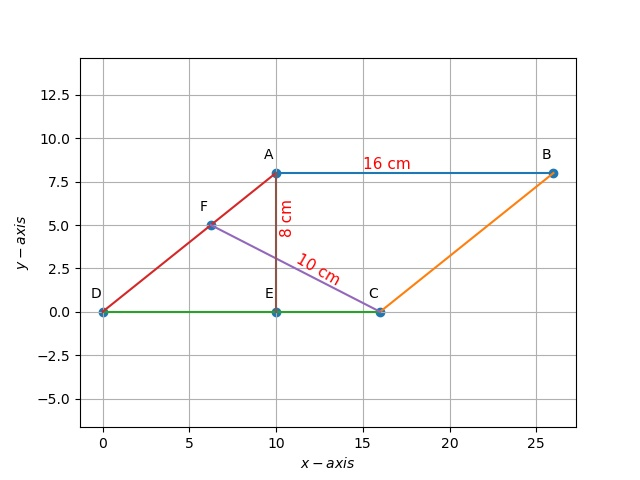
\includegraphics[width=0.5\textwidth]{fig 1.jpeg}
Figure 1 - Parallelogram ABCD


\section{Construction}
\vspace{0.5cm}
\begin{tabular}{|c|c|c|}
\hline
Symbol & Value & Description\\
\hline
D & Origin (0,0) & Vertex D \\
\hline
AB & 16cm & $\|\hspace{0.1cm} \vec{B} - \vec{A} \hspace{0.1cm}\|$ \\
\hline
CD & 16cm & $\|\hspace{0.1cm} \vec{D} - \vec{C} \hspace{0.1cm}\| = \|\hspace{0.1cm} \vec{B} - \vec{A} \hspace{0.1cm}\|$ \\
\hline
C & (16,0) & Vertex C ($\because CD = 16cm$)\\
\hline
AE & 8cm & $\|\hspace{0.1cm} \vec{E} - \vec{A} \hspace{0.1cm}\|$ \\
\hline

\end{tabular}
\begin{tabular}{|c|c|c|}

\hline
CF & 10cm & $\|\hspace{0.1cm} \vec{F} - \vec{C} \hspace{0.1cm}\|$ \\
\hline

A & (10,8) & Ay = Dy + $|\overrightarrow{AE}|$\\
 & & $Ax = \sqrt{\frac{CF^2}{AB^2 - CF^2}}$\\
 
\hline

B & (26,8) & By = Dy + $|\overrightarrow{AE}|$\\
 & & $Bx = Ax + AB$\\
 
\hline
F & (6.25,5) & $Fy = 0.8 \hspace{0.1cm} X\hspace{0.1cm} Fx$\\
\hline

E & (10,0) & Ex = Ax, Ey=0 \\
\hline

\end{tabular}


\section{Solution}
\raggedright
From the properties of Parallelogram we know that, Opposite sides are equal in length. Hence, we can write,\\
\vspace{0.25cm}
\centering
$|\hspace{0.1cm}\overrightarrow{CD}\hspace{0.1cm}| = |\hspace{0.1cm}\overrightarrow{AB}\hspace{0.1cm}|$\\
\vspace{0.25cm}
Hence,
$\|\hspace{0.1cm} \vec{D} - \vec{C} \hspace{0.1cm}\|\hspace{0.1cm} = \hspace{0.1cm} \|\hspace{0.1cm} \vec{B} - \vec{A}\hspace{0.1cm} \|\hspace{0.1cm}=\hspace{0.1cm}16cm$\\
\vspace{0.25cm}
\raggedright
We also know that,\\
\vspace{0.25cm}
\centering
Area of a Parallelogram = Base x Height\\
\vspace{0.25cm}
\raggedright
Since, it is given that $\overrightarrow{AE} \perp \overrightarrow{CD}$  from the figure 1 we can write,\\
\vspace{0.25cm}
Area of Parallelogram ABCD = $|\hspace{0.1cm} \overrightarrow{CD}\hspace{0.1cm}|\hspace{0.1cm} x\hspace{0.1cm}|\hspace{0.1cm}  \overrightarrow{AE}\hspace{0.1cm}|$ \hspace{0.1cm} (1)\\
\vspace{0.25cm}
\hspace{4.5cm} $=\hspace{0.1cm} \|\hspace{0.1cm} \vec{D} - \vec{C} \hspace{0.1cm}\|\hspace{0.1cm} x\hspace{0.1cm} \|\hspace{0.1cm} \vec{E} - \vec{A}\hspace{0.1cm} \|$\\
\vspace{0.25cm}
But it is also given that $\overrightarrow{CF} \perp \overrightarrow{AD}$. Hence we can similarly write,\\
\vspace{0.25cm}
Area of Parallelogram ABCD = $|\hspace{0.1cm} \overrightarrow{AD}\hspace{0.1cm}|\hspace{0.1cm}  x\hspace{0.1cm}|\hspace{0.1cm}  \overrightarrow{CF}\hspace{0.1cm}|$ \hspace{0.1cm} (2)\\
\vspace{0.25cm}
\hspace{4.5cm} $=\hspace{0.1cm} \|\hspace{0.1cm} \vec{D} - \vec{A} \hspace{0.1cm}\|\hspace{0.1cm} x\hspace{0.1cm} \|\hspace{0.1cm} \vec{F} - \vec{C}\hspace{0.1cm} \|$\\
\vspace{0.25cm}
Observing Eq. (1) and Eq. (2), we see that both are equal. Hence we get,\\
\vspace{0.25cm}
\centering

$ \|\hspace{0.1cm} \vec{D} - \vec{C} \hspace{0.1cm}\|\hspace{0.1cm} x\hspace{0.1cm} \|\hspace{0.1cm} \vec{E} - \vec{A}\hspace{0.1cm} \|\hspace{0.1cm} = \hspace{0.1cm} \|\hspace{0.1cm} \vec{D} - \vec{A} \hspace{0.1cm}\|\hspace{0.1cm} x\hspace{0.1cm} \|\hspace{0.1cm} \vec{F} - \vec{C}\hspace{0.1cm} \|  $

\vspace{0.25cm}

$|\hspace{0.1cm} 16\hspace{0.1cm}|\hspace{0.1cm}  x\hspace{0.1cm}|\hspace{0.1cm}  8 \hspace{0.1cm}|= \hspace{0.1cm}  \|\hspace{0.1cm} \vec{D} - \vec{A} \hspace{0.1cm}\| \hspace{0.1cm} x\hspace{0.1cm} |\hspace{0.1cm} 10\hspace{0.1cm}|$\\

\vspace{0.25cm}

128 = $\hspace{0.1cm} \|\hspace{0.1cm} \vec{D} - \vec{A} \hspace{0.1cm}\|\hspace{0.1cm}$ x 10\\

\vspace{0.25cm}

$ \|\hspace{0.1cm} \vec{D} - \vec{A} \hspace{0.1cm}\| \hspace{0.1cm}=\hspace{0.1cm}\frac{128}{10}$\\

\vspace{0.25cm}

$\therefore$ $|\hspace{0.1cm}$\textbf{$\overrightarrow{\vec{AD}}\hspace{0.1cm} |$ = 12.8 cm}\\

\vspace{0.25cm}

\centering
\textbf{Hence, This is the required value of AD.}

\vspace{0.25cm}


\end{document}
Footer

\item 
\iffalse
\documentclass[journal,10pt,twocolumn]{article}
\usepackage{graphicx}
\usepackage[margin=0.5in]{geometry}
\usepackage[cmex10]{amsmath}
\usepackage{array}
\usepackage{booktabs}
\title{\textbf{Line Assignment}}
\author{Mohamed Hamdan}
\date{September 2022}

\providecommand{\norm}[1]{\left\lVert#1\right\rVert}
\providecommand{\abs}[1]{\left\vert#1\right\vert}
\let\vec\mathbf
\newcommand{\myvec}[1]{\ensuremath{\begin{pmatrix}#1\end{pmatrix}}}
\newcommand{\mydet}[1]{\ensuremath{\begin{vmatrix}#1\end{vmatrix}}}
\providecommand{\brak}[1]{\ensuremath{\left(#1\right)}}

\begin{document}

\maketitle
\fi
 $ABC$ is a triangle right angled at $\vec{C}$. A line through the mid-point $\vec{M}$ of hypotenuse $AB$ and parallel to $BC$ intersects $AC$ at $D$ (see Fig.  
		\ref{fig:9/8/2/7}).
Show that
\begin{enumerate}
	\item $D$ is the mid-point of $AC$
	\item $MD \perp AC$
	\item $CM = MA = \frac{1}{2}AB$
\end{enumerate}
	\begin{figure}[!h]
		\centering
 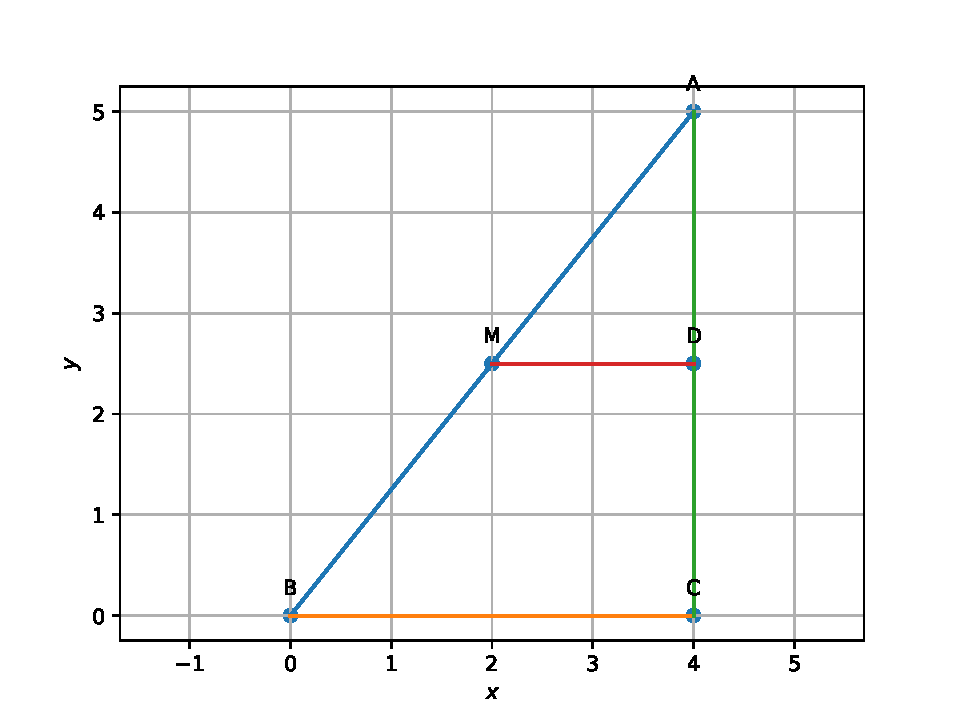
\includegraphics[width=\columnwidth]{chapters/9/8/2/7/figs/fig1.pdf}
		\caption{}
		\label{fig:9/8/2/7}
  	\end{figure}
	\solution 
	\begin{enumerate}
\item Trivial from  Appendix
		\label{prop:9/8/2/7}
	  \ref{prop:two-tri-bpt-conv}.
  \item 
Since $ABC$ is right angled at $C$,
\begin{equation}
	(\vec{C}-\vec{A})^{\top}(\vec{C}-\vec{B}) = 0	
\label{eq-3}
\end{equation}
Given that $MD$ is parallel to $BC$, so
\begin{equation}
	(\vec{C}-\vec{B}) = \lambda(\vec{M}-\vec{D})
\label{eq-4}
\end{equation}
Substituting (\ref{eq-4}) in (\ref{eq-3}) and dividing by $\lambda$, we get
\begin{equation}
	(\vec{C}-\vec{A})^{\top}(\vec{M}-\vec{D}) = 0	
\label{eq-5}
\end{equation}
From (\ref{eq-5}) it can be concluded that $MD \perp AC$.
\item Since
\begin{align}
	\norm{\vec{C}-\vec{M}}^2-\norm{\vec{A}-\vec{M}}^2 &= 	
	\norm{\vec{C}}^2-\norm{\vec{A}}^2-2\brak{\vec{C}-\vec{A}}^{\top}\vec{M} 
	\\
	&=\brak{\vec{C}-\vec{A}}^{\top}\brak{\vec{C}+\vec{A}-2\vec{M}} 
	\\
	&=\brak{\vec{C}-\vec{A}}^{\top}\brak{\vec{C}-\vec{B}} = \vec{0} 
\label{eq:9/8/2/7/sides}
\end{align}
upon substituting from 
Property		\ref{prop:9/8/2/7}
and 
\eqref{eq-3}.  Thus, $CM = AM$.

	\end{enumerate}

\iffalse
\section*{Solution}

\subsection*{Part 1}
Given MN is $\parallel$ to BC, hence\\
\begin{equation}
\frac{AD}{DC} = \frac{AM}{MB}
\label{eq-1}
\end{equation}
Since M is the mid-point of AB, $\frac{AM}{MB} = 1$. Substituting in (\ref{eq-1}), we get\\
\begin{equation}
AD = DC
\label{eq-2}
\end{equation}
Therefore, D is the midpoint of AC.

\subsection*{Part 2}
\subsection*{Part 3}
Let
\begin{eqnarray}
	\boldsymbol{M-D} = \boldsymbol{p}\\
	\boldsymbol{C-D} = \boldsymbol{q}\\
	\boldsymbol{A-D} = \boldsymbol{r}
\end{eqnarray}
Then vectors along CM and AM can be written as
\begin{eqnarray}
	\boldsymbol{C-M} = \boldsymbol{q-p}\\
	\boldsymbol{A-M} = \boldsymbol{r-p}
\end{eqnarray}
The magnitudes of CM and AM are therefore
\begin{eqnarray}
	||\boldsymbol{C-M}|| = ||\boldsymbol{q-p}|| = (\boldsymbol{q-p})^T(\boldsymbol{q-p})\\
	||\boldsymbol{A-M}|| = ||\boldsymbol{r-p}|| = (\boldsymbol{r-p})^T(\boldsymbol{r-p})\\
\end{eqnarray}
Upon expanding the vector products, the terms $\boldsymbol{q}^T\boldsymbol{p}$ and $\boldsymbol{r}^T\boldsymbol{p}$ evaluate to 0 (from eq.\ref{eq-5}). From eq.\ref{eq-2}, $$||\boldsymbol{q}|| = ||\boldsymbol{r}||$$. Therefore,
\begin{equation}
||\boldsymbol{C-M}|| = ||\boldsymbol{q}|| + ||\boldsymbol{p}||\\
\label{eq-4-}
\end{equation}
\begin{equation}
||\boldsymbol{A-M}|| = ||\boldsymbol{r}|| + ||\boldsymbol{p}|| = ||\boldsymbol{q}|| + ||\boldsymbol{p}||
\label{eq-3-}
\end{equation}
Equating (\ref{eq-4-}) and (\ref{eq-3-}), we get
\begin{equation}
AM = CM
\label{eq-2-}
\end{equation}
Since given that M is midpoint of AB, 
\begin{equation}
AM = \frac{1}{2}AB
\label{eq-1-}
\end{equation}
Equating (\ref{eq-2-}) and (\ref{eq-1-}), the result is proved.

\section*{Construction}
The input parameters are the lengths a and c.\\
{
\setlength\extrarowheight{2pt}
\begin{tabular}{|c|c|c|}
	\hline
	\textbf{Symbol}&\textbf{Value}&\textbf{Description}\\
	\hline
	a&4&BC\\
	\hline
	c&5&AC\\
	\hline
	k&1&$\frac{AM}{MB} = \frac{AD}{DC}$\\
	\hline
	$\theta$&arctan($\frac{c}{a}$)&$\angle$B\\
	\hline
	A&$\sqrt{a^2+c^2}%
	\begin{pmatrix}
		cos\theta\\
		sin\theta\\
	\end{pmatrix}$%
	&Point A\\
	\hline
\end{tabular}
}

\section*{Proofs}
Let the vertices of the triangle be $\vec{A}, \vec{B}, \vec{C}$ such that  
		\begin{align}
			\vec{B} =\vec{0} 
		\end{align}
		and $\vec{A}, \vec{C}$ are known. Let $\vec{P}$ be a known point on $AB$ such that $PQ$ is parallel to $BC$.  Let 
		\begin{align}
			\vec{P} &= \lambda \brak{\vec{A} -\vec{B} }
			\label{eq:cbse-2020-10-bpty}
			\\
			&=\lambda 
			 \vec{A} 
			\label{eq:cbse-2020-10-bpt}
			\\
			\text{and , } \frac{\norm{\vec{P} 
			}}{\norm{\vec{A}} } &= \frac{BP}{AB}= \abs{\lambda}
			\label{eq:cbse-2020-10-bpt-pa}
		\end{align}
		Since 
		\begin{align}
			PQ &\parallel BC,
			\\
			\vec{Q} &= P + \mu \vec{B-C}
			\\
			&= \lambda \vec{A} - \mu \vec{C}
			\label{eq:cbse-2020-10-bpt-q1}
		\end{align}
		using the equation of the line $PQ$  and substituting from 
			\eqref{eq:cbse-2020-10-bpt}
			Also, since $\vec{Q}$  lies on the line $AC$, 
		\begin{align}
			\vec{Q} &= \vec{A} + k \brak{\vec{A}-\vec{C}}
			\\
			&= \brak{1 + k}\vec{A} - k \vec{C}
			\label{eq:cbse-2020-10-bpt-q2}
			\\
			\text{and }\frac{\norm{{\vec{A}-\vec{Q}}}}{\norm{{\vec{A}-\vec{C}}}} &= \frac{AQ}{AC}= \abs{k}
			\label{eq:cbse-2020-10-bpt-q2k}
		\end{align}
			From \eqref{eq:cbse-2020-10-bpt-q1} and 
			\eqref{eq:cbse-2020-10-bpt-q2}
		\begin{align}
			\lambda \vec{A} - \mu \vec{C}	= 
			 \brak{1 + k}\vec{A} - k \vec{C}&
			\\
			\implies 
			\brak{1 + k+\lambda }\vec{A} \brak{k - \mu}  \vec{C}	&=  0
			\\
			\implies k = \mu, \lambda = -1 - \mu 
			\\
			\text{or, } \abs{\lambda } = 1 + k
			\label{eq:cbse-2020-10-bpt-q2-lk}
		\end{align}
		From 
			\eqref{eq:cbse-2020-10-bpt-pa},  
			\eqref{eq:cbse-2020-10-bpt-q2k} and
			\eqref{eq:cbse-2020-10-bpt-q2-lk},
			\begin{align}
				\frac{AQ}{AC} = \frac{AP}{AB}
			\end{align}
\end{document}
\fi

\iffalse
\item 
\iffalse
 

\def\mytitle{MATRICES USING PYTHON}
\def\myauthor{THOUTU RAHUL RAJ}
\def\contact{rdj4648@gmail.com}
\def\mymodule{Future Wireless Communication (FWC)}
\documentclass[10pt, a4paper]{article}
\usepackage[a4paper,outer=1.5cm,inner=1.5cm,top=1.75cm,bottom=1.5cm]{geometry}
\twocolumn
\usepackage{graphicx}
\graphicspath{{./images/}}
\usepackage[colorlinks,linkcolor={black},citecolor={blue!80!black},urlcolor={blue!80!black}]{hyperref}
\usepackage[parfill]{parskip}
\usepackage{lmodern}
\usepackage{amsmath,amsfonts,amssymb,amsthm}
\usepackage{tikz}
	\usepackage{physics}
%\documentclass[tikz, border=2mm]{standalone}
\usepackage{karnaugh-map}
%\documentclass{article}
\usepackage{tabularx}
\usepackage{circuitikz}
\usetikzlibrary{calc}
\usepackage{amsmath}
\usepackage{amssymb}
\renewcommand*\familydefault{\sfdefault}
\usepackage{watermark}
\usepackage{lipsum}
\usepackage{xcolor}
\usepackage{listings}
\usepackage{float}
\usepackage{titlesec}
\providecommand{\norm}[1]{\left\lVert#1\right\rVert}
\providecommand{\sbrak}[1]{\ensuremath{{}\left[#1\right]}}
\providecommand{\lsbrak}[1]{\ensuremath{{}\left[#1\right.}}
\providecommand{\rsbrak}[1]{\ensuremath{{}\left.#1\right]}}
\providecommand{\brak}[1]{\ensuremath{\left(#1\right)}}
\providecommand{\lbrak}[1]{\ensuremath{\left(#1\right.}}
\providecommand{\rbrak}[1]{\ensuremath{\left.#1\right)}}
\providecommand{\cbrak}[1]{\ensuremath{\left\{#1\right\}}}
\providecommand{\lcbrak}[1]{\ensuremath{\left\{#1\right.}}
\providecommand{\rcbrak}[1]{\ensuremath{\left.#1\right\}}}
\newcommand{\myvec}[1]{\ensuremath{\begin{pmatrix}#1\end{pmatrix}}}
\let\vec\mathbf
\providecommand{\mtx}[1]{\mathbf{#1}}
\titlespacing{\subsection}{1pt}{\parskip}{3pt}
\titlespacing{\subsubsection}{0pt}{\parskip}{-\parskip}
\titlespacing{\paragraph}{0pt}{\parskip}{\parskip}
\newcommand{\figuremacro}[5]

\begin{document}

\title{\mytitle}
\author{\myauthor\hspace{1em}\\\contact\\FWC22008\hspace{6.5em}IITH\hspace{0.5em}\mymodule\hspace{6em}ASSIGN-4}
\date{}
	\maketitle
		
	\tableofcontents
\vspace{5mm}
\fi
If diagonals of a parallelogram are equal then show that it is a rectangle.

	\begin{figure}[!h]
		\centering
		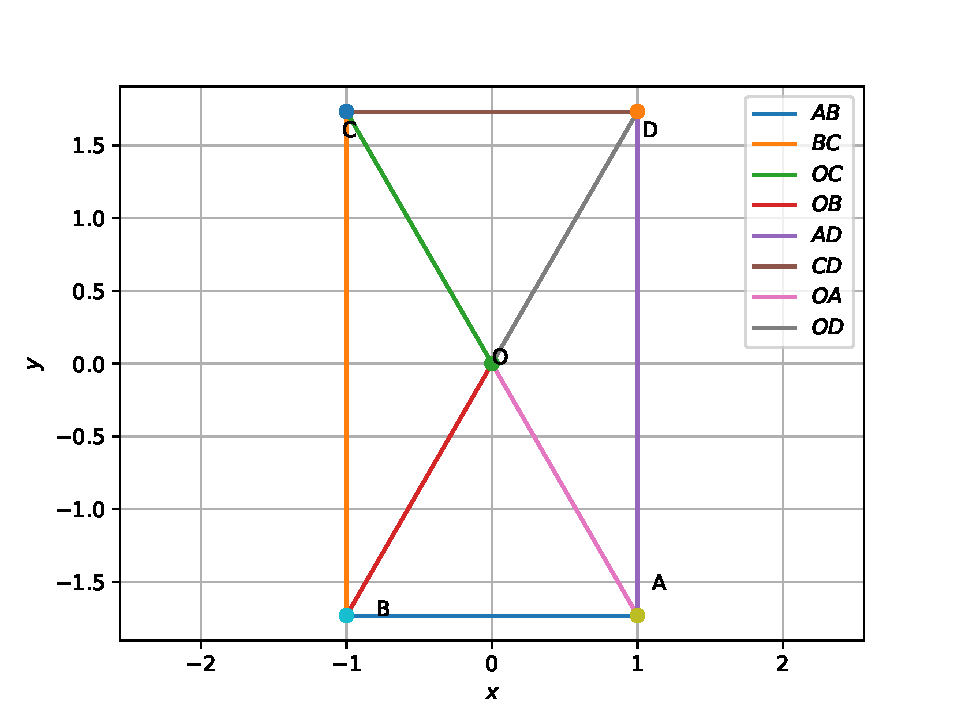
\includegraphics[width=\columnwidth]{chapters/9/8/1/2/fig.pdf}
     %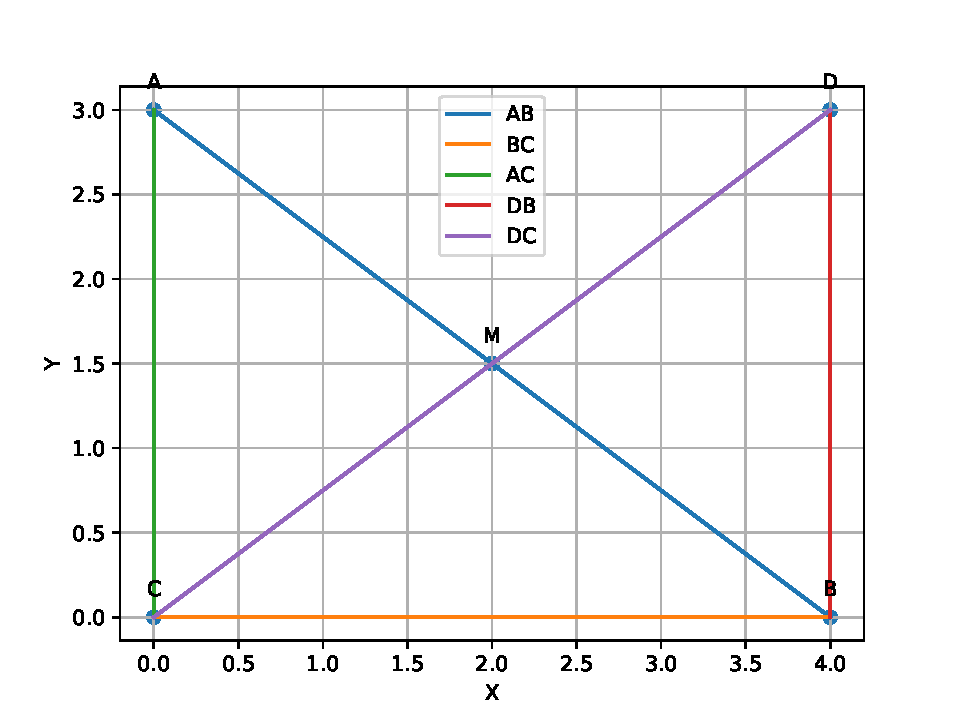
\includegraphics[scale=0.5]{fig.pdf} 
		\caption{}
		\label{fig:9/8/1/2}
  	\end{figure}
	\solution 
   See Fig. 
		\ref{fig:9/8/1/2}.
   From 
	  \eqref{eq:two-pgm}, 
\begin{align}
	  \label{eq:two-pgm-def} 
 \vec{B} - \vec{A}= \vec{C}-\vec{D}
 \\
\implies  \vec{B} - \vec{C}= \vec{A}-\vec{D}
	\end{align}
	Also, it is given that the diagonals of $ABCD$ are equal.  Hence, 
\begin{align}
	\norm{\vec{C} - \vec{A}}^2&= \norm{\vec{D}-\vec{B}}^2
 \\
	\implies 
	\norm{(\vec{C}-\vec{B}) + (\vec{B}-\vec{A})}^2 &= \norm{(\vec{D}-\vec{C}) + (\vec{C}-\vec{B}}^2
\end{align}
which can be expressed as
\begin{multline}
	\norm{\vec{C}-\vec{B}}^2 + \norm{\vec{B}-\vec{A}}^2 + 2(\vec{C}-\vec{B})^{\top} (\vec{B}-\vec{A}) 
	\\
	= \norm{\vec{D}-\vec{C}}^2 + \norm{\vec{C}-\vec{B}}^2+2(\vec{D}-\vec{C})^{\top} (\vec{C}-\vec{B}) 
\end{multline}
which, can be simplified to obtain 
\begin{align}
	(\vec{C}-\vec{B})^{\top} (\vec{B}-\vec{A})&=(\vec{D}-\vec{C})^{\top} (\vec{C}-\vec{B}) 
\end{align}
since 
\begin{align}
\norm{\vec{D}-\vec{C}} =   
\norm{\vec{B}-\vec{A}}   
\end{align}
yielding 
\begin{align}
	(\vec{A}-\vec{B})^{\top} (\vec{B}-\vec{C})=\vec{0}
\end{align}
	  from \eqref{eq:two-pgm-def}.  

\item 
\label{chapters/9/8/1/3}
\iffalse
\documentclass[a4paper,12pt,twocolumn]{article}
\usepackage{graphicx}
\usepackage[margin=0.5in]{geometry}
\usepackage[cmex10]{amsmath}
\usepackage{array}
\usepackage{gensymb}
\usepackage{booktabs}
\title{Line Assignment}

\author{Ravi Sumanth Muppana- FWC22003}
\date{September 2022}
\providecommand{\norm}[1]{\left\lVert#1\right\rVert}
\providecommand{\abs}[1]{\left\vert#1\right\vert}
\let\vec\mathbf
\newcommand{\myvec}[1]{\ensuremath{\begin{pmatrix}#1\end{pmatrix}}}	
\newcommand{\mydet}[1]{\ensuremath{\begin{vmatrix}#1\end{vmatrix}}}
\providecommand{\brak}[1]{\ensuremath{\left((#1\right)}}
\begin{document}
\maketitle
\section{Problem:}
\fi
Show that if the diagonals of a quadrilateral bisect each other at right angles, then it is a rhombus.
\begin{figure}[!h]
	\centering
	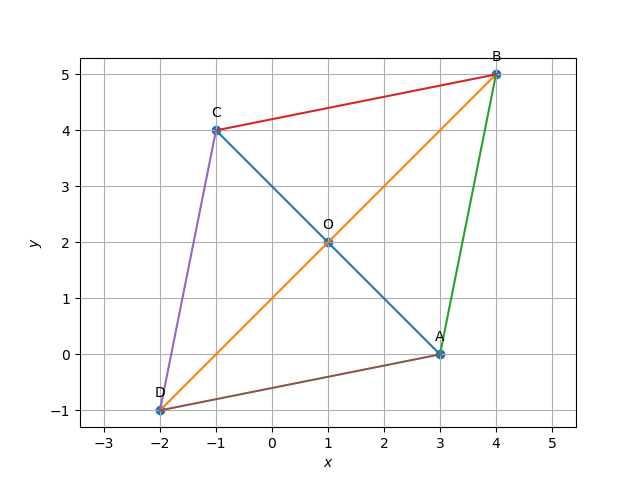
\includegraphics[width=\columnwidth]{chapters/9/8/1/3/figs/rhombus.png}
	\caption{Rhombus}
	\label{fig:9/8/1/3}
\end{figure}
\\
\solution See Fig. 
	\ref{fig:9/8/1/3}.
\iffalse
\maketitle
\section{Solution:}
\subsection{Theory:}
\fi
From the given information,
\begin{align}
	\label{eq:9/8/1/3-mid}
	\frac{\vec{B}+\vec{D}}{2}
	&=	
	\frac{\vec{A}+\vec{C}}{2}
	\\
	\brak{\vec{B}-\vec{D}}^{\top}&
	\brak{\vec{A}-\vec{C}} = 0
	\label{eq:9/8/1/3-orth}
\end{align}
From 
	\eqref{eq:9/8/1/3-mid},
\begin{align}
	\vec{B}-\vec{A}
	=	
	\vec{C}-\vec{D}
	\label{eq:9/8/1/3-pgm}
\end{align}
which, from  
	  \eqref{eq:two-pgm}, 
is the definition of  a parallelogram.
Further, substituting
\begin{align}
	\vec{B}-\vec{D} &= \brak{\vec{B}-\vec{A}} +  
	\brak{\vec{A}-\vec{D}}
	\\
	\vec{A}-\vec{C} &= \brak{\vec{A}-\vec{B}} +  
	\brak{\vec{B}-\vec{C}}
\end{align}
in 
	\eqref{eq:9/8/1/3-orth},  
\begin{multline}
	\sbrak{\brak{\vec{B}-\vec{A}} +  
	\brak{\vec{A}-\vec{D}}}^{\top}
	\sbrak{ \brak{\vec{A}-\vec{B}} +  
	\brak{\vec{B}-\vec{C}}} = 0
	\\
	\implies 
-\norm{\vec{B}-\vec{A}}^2 + \brak{\vec{B}-\vec{A}}^{\top}\brak{\vec{B}-\vec{C}} + 
\\
	\brak{\vec{A}-\vec{D}}^{\top}\brak{\vec{A}-\vec{B}} + 
\brak{\vec{A}-\vec{D}}^{\top}
\brak{\vec{B}-\vec{C}} = 0
	\label{eq:9/8/1/3-org}
\end{multline}
From
	\eqref{eq:9/8/1/3-pgm},
\begin{align}
	\vec{B}-\vec{C}
	=	
	\vec{A}-\vec{D}
	\\
	\implies \brak{\vec{B}-\vec{A}}^{\top}\brak{\vec{B}-\vec{C}} +
	 \brak{\vec{A}-\vec{D}}^{\top}\brak{\vec{A}-\vec{B}} =\vec{0}
	\label{eq:9/8/1/3-orth-pf}
\end{align}
and 
\begin{align}
\brak{\vec{A}-\vec{D}}^{\top}
\brak{\vec{B}-\vec{C}} = \norm{\vec{B}-\vec{C}}^2
	\label{eq:9/8/1/3-orth-eq}
\end{align}
Substituting from

	\eqref{eq:9/8/1/3-orth-pf}
and
	\eqref{eq:9/8/1/3-orth-eq}
in
	\eqref{eq:9/8/1/3-org},

\begin{align}
\norm{\vec{A}-\vec{B}}^{2}
= \norm{\vec{B}-\vec{C}}^2
\end{align}
which means that the adjacent sides of the parallelogram are equal. Thus, the quadrilateral is a rhombus
\iffalse


Since
Let us assume two vectors $\vec{C}-\vec{B}-\vec{A}$ and $\vec{C}-\vec{B}$ for sides $BA$ and $CB$. The diagonals $AC,BD$ are the addition and subtraction of the two vectors:
\begin{align}
	&\vec{(B-A)} = \vec{C}-\vec{B}-\vec{A}\\
	&\vec{(C-B)} = \vec{C}-\vec{B}\\
	&\vec{(C-A)} = \vec{(C-B)} +\vec{(B-A)}\\
	&\vec{(C-A)} = \vec{b+a}\\
	&\vec{(D-B)} = \vec{b-a}\\
\end{align}
%\subsection{Mathematical Calculation:}
Let the two diagonals be $\vec{a+b}$, $\vec{b-a}$. Since the diagonals are at right angle to each other,
\begin{align}
&0 = \vec{(a+b)^T}\vec{(b-a)}\\	
&||\vec{C}-\vec{B}||^2 - ||\vec{C}-\vec{B}-\vec{A}||^2 = 0\\
&||\vec{C}-\vec{B}|| = ||\vec{C}-\vec{B}-\vec{A}||\\
\end{align}
Hence, the two sides of the quadrilateral are equal. We need to prove the third side is also equal.
Now,
In triangle BOA and AOD;
\begin{align}
	&\vec{B-O} = \vec{p}\\
	&\vec{D-O} = \vec{-p}\\
	&\vec{A-O} = \vec{r}\\
\end{align}
\begin{align}
	&\vec{C}-\vec{B}-\vec{A} = \vec{(B-O)} - \vec{(A-O)}\\ 
	&\vec{d} = \vec{(D-O)} - \vec{(A-O)}\\
&||\vec{C}-\vec{B}-\vec{A}||^2 = ||\vec{p}||^2 + ||\vec{r}||^2 - 2\vec{p^Tr}\\
&||\vec{d}||^2 = ||\vec{-p}||^2 + ||\vec{r}||^2 + 2\vec{p^Tr}\\
\end{align}
The terms $\vec{p^Tr}$ is equal to zero as they is perpendicular.Therefore,
\begin{align}
	&||\vec{C}-\vec{B}-\vec{A}||^2 = ||\vec{p}||^2 + ||\vec{r}||^2\\
	&||\vec{d}||^2 = ||\vec{p}||^2 + ||\vec{r}||^2\\
	&Clearly, ||\vec{C}-\vec{B}-\vec{A}|| = ||\vec{d}||\\
\end{align}
Hence, all three sides are equal, it's a parallelogram. A parallelogram with it's diagonals as perpendicular bisectors is a rhombus.
\fi
\iffalse
\section{Construction:}
Consider any  three vertices of the rhombus. Using the vertices, find the midpoint of the diagonals, then find the fourth point using the midpoint and remaining vertex. 
\begin{table}[h]
	\centering
\setlength\extrarowheight{2pt}
	\begin{tabular}{|c|c|c|}
		\hline
		\textbf{variable} & \textbf{length/point} & \textbf{Description}\\
		\hline
		A & [3,0] & Vertex A\\
		\hline
		B & [4,5] & Vertex B\\
		\hline
		C & [-1,4] & Vertex C\\
		\hline                   
		D & [D-x,D-y] & Vertex D\\
		\hline
		M & (A+B)/2 & midpoint\\
		\hline
		(D-x,D-y) & (2*M[0]-B[0],2*M[1]-B[1]) & vertex of D\\
		\hline
	\end{tabular}
\end{table}

\end{document}
\fi

\item 
\iffalse
\documentclass[journal,12pt,twocolumn]{article}
\usepackage{graphicx}
\usepackage[none]{hyphenat}
\usepackage[margin=0.5in]{geometry}
\usepackage[cmex10]{amsmath}
\usepackage{array}
\usepackage{booktabs}
\usepackage{gensymb}
\usepackage{textcomp}
\title{\textbf{Line Assignment}}
\author{Manideep Parusha - FWC22004}
\date{\today}

\providecommand{\norm}[1]{\left\lVert#1\right\rVert}
\providecommand{\abs}[1]{\left\vert#1\right\vert}
\let\vec\mathbf
\newcommand{\myvec}[1]{\ensuremath{\begin{pmatrix}#1\end{pmatrix}}}
\newcommand{\mydet}[1]{\ensuremath{\begin{vmatrix}#1\end{vmatrix}}}
\providecommand{\brak}[1]{\ensuremath{\left(#1\right)}}

\begin{document}

\maketitle
\section*{Problem}
\fi
Show that the diagonals of a square are equal and bisect each other at right angles.
\solution This is obvious from Problems
\eqref{chapters/9/8/1/2}
and
\eqref{chapters/9/8/1/3}.

\iffalse
\section*{Solution}

\begin{figure}[h]
\centering
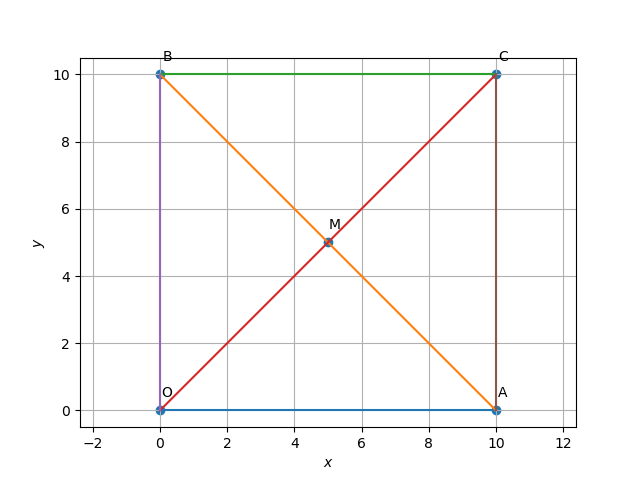
\includegraphics[width=\columnwidth]{figs/sq_plot.png}
\caption{Square generated using python}
\label{fig:sq_py}
\end{figure}

\subsection*{Construction}
Inputs taken for the construction of the Square is 'a' , which is the side length of the square.
\begin{table}[h]
	\centering
\setlength\extrarowheight{2pt}
	\begin{tabular}{|c|c|c|}
		\hline
		\textbf{Symbol} & \textbf{Value} & \textbf{Description} \\
		\hline
		a & 10 & length of OA\\
		\hline
		O & (0,0) & point O\\
		\hline
		A & (a,0) & point A\\
		\hline
		B & (0,a) & point B\\
		\hline
		C & A+B & point C\\
		\hline
		M & $\frac{C}{2}$ & point M\\
		\hline
	\end{tabular}
\end{table}


Let OABC is a Square. Length of all sides are equal for a square and all interior angles equal to 90\degree.
O at the origin and vectors A, B \& C represent other vertices of the square.
\begin{align}
	\norm{\boldsymbol{OA}} = \norm{\boldsymbol{OB}} = \norm{\boldsymbol{BC}} = \norm{\boldsymbol{AC}} \\
\angle OAC = \angle OBC = \angle BCA = \angle AOB = 90\degree
\label{eq-1}
\end{align}
Here, $D_1$ and $D_2$ are the diagonals of the square and we can compute $D_1$ and $D_2$ as
\begin{equation}
	\boldsymbol{D_1 = (A + B) } \\
	\label{D1eq}
\end{equation}
\begin{equation}
	\boldsymbol{D_2 = (A - B) }
	\label{D2eq}
\end{equation}

To prove that the diagonals of the square are equal, we can find the length of the two diagonals and compare. Hence,
\begin{equation}
\norm {\boldsymbol{D_1}}  = \norm {\boldsymbol{A + B}}\\
	\label{D1_len}
\end{equation}
\begin{equation}
\norm {\boldsymbol{D_2}}  = \norm {\boldsymbol{A - B}}
	\label{D2_len}
\end{equation}
For finding length of $D_1$, we can write from equation \eqref{D1_len},  
\begin{align}
	\norm{\boldsymbol{A + B}} = \sqrt{\norm{\boldsymbol{A}}^2 + \norm{\boldsymbol{B}}^2 + 2\boldsymbol{A}^T\boldsymbol{B}}
	\label{extend_D1}
\end{align}
But, for a square we know that length of all sides are equal.
\begin{equation}
	\norm {\boldsymbol{A}} = \norm{\boldsymbol{B}}
	\label{equal_sides}
\end{equation}
and, the angle between two adjacent sides is 90\degree. The dot product of two vectors which are seperated by 90\degree angle is always '0'. 
\begin{equation}
	\boldsymbol{A}^T\boldsymbol{B} = 0 
	\label{dot_product_is_0}
\end{equation}
So the equation \eqref{extend_D1} becomes 
\begin{align}
	\norm {\boldsymbol{A + B}} = \sqrt{2}\norm{\boldsymbol{A}}\\
	\norm {\boldsymbol{D_1}} = \sqrt{2}\norm{\boldsymbol{A}} 
	\label{D1_length}
\end{align}
Similarly, for finding the length of $D_2$ 
\begin{align}
	\norm {\boldsymbol{A - B}} = \sqrt{\norm{\boldsymbol{A}}^2 + \norm{\boldsymbol{B}}^2 - 2\boldsymbol{A}^T\boldsymbol{B}}
\end{align}
But, from \eqref{equal_sides} and \eqref{dot_product_is_0}
\begin{align}
	\norm {\boldsymbol{A - B}} = \sqrt{2}\norm{\boldsymbol{A}}\\
	\norm {\boldsymbol{D_2}} = \sqrt{2}\norm{\boldsymbol{A}} 
	\label{D2_length}
\end{align}
So, from the equations \eqref{D1_length} and \eqref{D2_length}, we can say that the lengths of diagonals $\boldsymbol{D_1}$ and $\boldsymbol{D_2}$ are equal 
\begin{equation}
	\norm{\boldsymbol{D_1}} = \norm{\boldsymbol{D_2}}
\end{equation}





We know that, if the dot product of two vectors is zero then the vectors are perpendicular to each other. \\
So, by taking the dot product of $\boldsymbol{D_1}$ and $\boldsymbol{D_2}$ 
\begin{align}
	\boldsymbol{D_1.D_2} = \boldsymbol{D_1}^T \boldsymbol{D_2} \\
	\boldsymbol{D_1.D_2} = (\boldsymbol{A + B})^T(\boldsymbol{A - B})\\
	\boldsymbol{D_1.D_2} = \norm{\boldsymbol{A}}^2 - \norm{\boldsymbol{B}}^2
\end{align}	
From the equation \eqref{equal_sides}, 
\begin{align}
	\boldsymbol{D_1.D_2} = \norm{\boldsymbol{A}}^2 - \norm{\boldsymbol{A}}^2 \\
	\boldsymbol{D_1.D_2} = 0 
\end{align}	
as the dot product of the diagonals is equal to 0, we can say that both diagonals are perpendicular to each other. \\

Let diagonals $\boldsymbol{D_1}$ and $\boldsymbol{D_2}$ intersect at a point $\boldsymbol{M}$. We have to prove that $\boldsymbol{M}$ is the mid point of $\boldsymbol{D_1}$ and $\boldsymbol{D_2}$, in order to say that both diagonals bisect eachother.
\begin{align}
	\boldsymbol{OM} = x \boldsymbol{D_1}\\
	\boldsymbol{MA} = y \boldsymbol{D_2}
\end{align}
From the equations \eqref{D1eq} and \eqref{D2eq}, the above equations can be written as
\begin{align}
	\boldsymbol{OM} = x\boldsymbol{A + B}\\
	\boldsymbol{MA} = y\boldsymbol{A - B}
\end{align}
Now, if we consider
\begin{align}
	\boldsymbol{OA} = \boldsymbol{OM} + \boldsymbol{MA}\\
	\boldsymbol{A} = x(\boldsymbol{A+B}) + y(\boldsymbol{A-B})\\
	\boldsymbol{A} = x\boldsymbol{A} + x\boldsymbol{B} + y\boldsymbol{A} - y\boldsymbol{B}\\
	\boldsymbol{A} = (x+y)\boldsymbol{A} + (x-y)\boldsymbol{B}
\end{align}
Equating the co-efficient of $\boldsymbol{A}$ and $\boldsymbol{B}$, we get
\begin{align}
	x + y = 1 , x - y = 0\\
	2x = 1\\
	x = \frac{1}{2}\\
	y = \frac{1}{2}
\end{align}

now we can say that
\begin{align}
	\boldsymbol{OM} = \frac{1}{2} \boldsymbol{D_1}\\
	\boldsymbol{MA} = \frac{1}{2} \boldsymbol{D_2}
\end{align}
Hence, M is the mid point of diagonals $D_1$ and $D_2$ and we can say that both diagonals bisect eachother. \\

we have proved that diagonals of a square are equal in length and bisect eachother at right angles.





\end{document}
\fi

\item 
\item 
\iffalse
\documentclass[a4paper,12pt,twocolumn]{article}
\usepackage{graphicx}
\usepackage[margin=0.5in]{geometry}
\usepackage[cmex10]{amsmath}
\usepackage{array}
\usepackage{gensymb}
\usepackage{booktabs}
\usepackage{tabularx}
\title{Line Assignment}

\author{Ginna Shreyani- FWC22006}
\date{September 2022}
\providecommand{\norm}[1]{\left\lVert#1\right\rVert}
\providecommand{\abs}[1]{\left\vert#1\right\vert}
\let\vec\mathbf
\newcommand{\myvec}[1]{\ensuremath{\begin{pmatrix}#1\end{pmatrix}}}	
\newcommand{\mydet}[1]{\ensuremath{\begin{vmatrix}#1\end{vmatrix}}}
\providecommand{\brak}[1]{\ensuremath{\left((#1\right)}}
\begin{document}
\maketitle
\section{Problem:}
\fi
Diagonal AC of a parallelogram ABCD bisects $\angle{A}$ in Fig \eqref{fig:9/8/1/6}. Show that 
\begin{enumerate}
	\item	it bisects $\angle{C}$ also
	\item $ABCD$ is a rhombus
\end{enumerate}
\begin{figure}[!h]
	\centering
	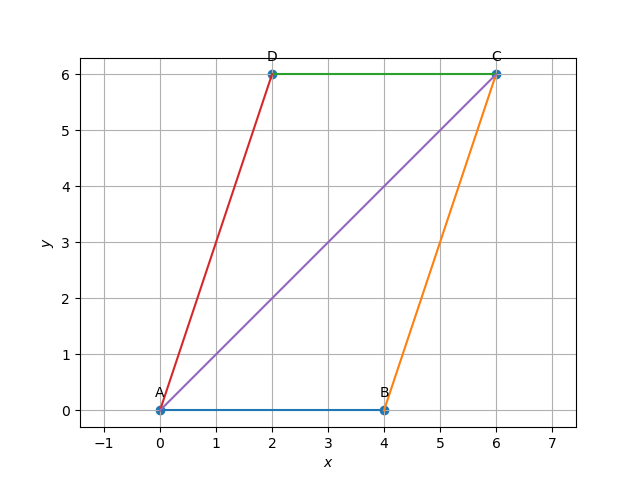
\includegraphics[width=\columnwidth]{chapters/9/8/1/6/figs/parallel.png}
	\caption{}
	\label{fig:9/8/1/6}
\end{figure}
\solution  
\iffalse
are given by 
\begin{proof}
Any point on the angle bisector is equidistant from the lines.  
\end{proof}
\fi	
%\item ({\em Reflection }) Assuming that straight lines work as a plane mirror for a point, find the image of the point $\vec{P}=\myvec{1\\2}$ in the line 
%%
\iffalse
\maketitle
\section{Construction:}
\begin{tabularx}
{0.5\textwidth}{
|>
{\raggedright\arraybackslash}X
|>
{\centering\arraybackslash}X
|>
{\raggedleft\arraybackslash}X
|}
\hline
 Variable & Point/Length & Description\\
\hline
 A  &  $\myvec{0\\0}$ & Vertex A\\
 \hline
 B & $\myvec{4\\0}$ & Vertex B\\
 \hline
 C & $\myvec{6\\6}$ & Vertex C\\
 \hline
 D & $\myvec{2\\6}$ & Vertex D\\
 \hline
\end{tabularx}
\maketitle
\section{Solution:}
\subsection{Theory:}
Given a diagonal of a parallelogram bisects an angle,we need to prove that the same diagonal bisects the opposite angle of the parallelogram by using vector algebra.\\
\subsection{Mathematical Calculation:}
Here the diagonal joining vertices A and C  can be represented as
\begin{equation}
\vec{C}-\vec{A} = \vec{B}-\vec{A}+\vec{C}-\vec{B}
\end{equation}
The other diagonal joining vertices B and D can be represented as
\begin{equation}
\vec{D-B} = \vec{B}-\vec{C}-\vec{B}-\vec{A}
\end{equation}
$\boldsymbol{(i)}$ Let the $\angle{CAB}$  be $\theta_1$ and the $\angle{DAC}$  be $\theta_2$ and the $\angle{DCA}$  be $\theta_3$ and $\angle{ACB}$ be $\theta_4$\\
Since the diagonal $\vec{C}-\vec{A}$ bisects $\angle{A}$, $\angle{CAB} = \angle{DAC}$,therefore we get $\theta_1=\theta_2$\\
\fi
\begin{enumerate}
	\item From 
    \eqref{eq:angle2d},
\begin{align}
	 \label{eq:9/8/1/6/bis}
	\angle{BAC}
	&= \angle{DAC}
	\\
\implies  \frac{(\vec{A}-\vec{B})^T(\vec{A}-\vec{C})}{\norm{\vec{A}-\vec{B}}\norm{\vec{A}-\vec{C}}}
	& = \frac{(\vec{A}-\vec{D})^T(\vec{A}-\vec{C})}{\norm{\vec{A}-\vec{D}}\norm{\vec{A}-\vec{C}}}
%
%&cos\theta_3 = \frac{\vec{-(B-A)}^T\vec{-(C-A)}}{\vec{||-(B-A)||}.\vec{||-(C-A)||}}\\
%&cos\theta_3 = \frac{\brak{vec{B}-\vec{A}}^T\brak{vec{C}-\vec{A}}}{\vec{||B-A||}.\vec{||C-A||}}\\
%&cos\theta_1 = cos\theta_3\\
%&\theta_1=\theta_3
\end{align}
Also, 
\begin{align}
\cos	\angle{ACD}
	 = \frac{(\vec{C}-\vec{D})^T(\vec{C}-\vec{A})}{\norm{\vec{C}-\vec{D}}\norm{\vec{C}-\vec{A}}}
	 \label{eq:9/8/1/6/cang}
%
\end{align}
From Appendix
	  \ref{eq:two-pgm}, 
  \begin{align}
	  \vec{B}-\vec{A} &= \vec{C} -\vec{D}
	  \\
	  \implies 
	  \frac{(\vec{C}-\vec{D})^T(\vec{C}-\vec{A})}{\norm{\vec{C}-\vec{D}}\norm{\vec{C}-\vec{A}}}
	  &= \frac{(\vec{B}-\vec{A})^T(\vec{C}-\vec{A})}{\norm{\vec{B}-\vec{A}}\norm{\vec{C}-\vec{A}}}
	 \label{eq:9/8/1/6/rh}
  \end{align}
  upon substituting in 
	 \eqref{eq:9/8/1/6/cang}. Thus, from 
	 \eqref{eq:9/8/1/6/cang}
	 and 
	 \eqref{eq:9/8/1/6/bis}, 
\begin{align}
	\angle{BAC}
	= \angle{DAC}
	=
	\angle{ACD}
  \end{align}
  Similarly, it can be shown that 
  \begin{align}
	\angle{ACD}
	=
	\angle{ACB}
  \end{align}
  \item 
  \iffalse
From 
	 \eqref{eq:9/8/1/6/rh}, 
  \begin{align}
	  \frac{(\vec{C}-\vec{D})^T(\vec{C}-\vec{A})}{\norm{\vec{C}-\vec{D}}\norm{\vec{C}-\vec{A}}}
	  &= \frac{(\vec{B}-\vec{A})^T(\vec{C}-\vec{A})}{\norm{\vec{B}-\vec{A}}\norm{\vec{C}-\vec{A}}}
  \end{align}
The equation of the bisector of $\angle BAD$ is given by Appendix  
	\ref{prob:ang-bisect} as
\begin{align}
	 \label{eq:9/8/1/6/ac}
	\frac{\vec{n}_1^{\top}\vec{x} - c_1}{\norm{\vec{n}_1}}
	= 
	\frac{\vec{n}_2^{\top}\vec{x} - c_2}{\norm{\vec{n}_2}}
\end{align}
where the equations of $AB, AD$ are respectively given by 
\begin{align}
	\vec{n}_1^{\top}\vec{x} &= c_1
	\\
	\vec{n}_2^{\top}\vec{x} &= c_2
\end{align}
From 
    \eqref{eq:dir_vec}
    and 
    \eqref{eq:normal_vec}, 
\begin{align}
	 \label{eq:9/8/1/6/orth}
	\vec{n}_1^{\top}\brak{\vec{A}-\vec{B}} &= 0
	\\
	\vec{n}_2^{\top}\brak{\vec{A}-\vec{D}}&= 0
\end{align}
%
From 
	 \eqref{eq:9/8/1/6/ac}, the normal vector of $AC$ is 
\begin{align}
	\frac{\vec{n}_1}{\norm{\vec{n}_1}}
	&- 
	\frac{\vec{n}_2}{\norm{\vec{n}_2}}
	\\
	\implies
	\brak{\frac{\vec{n}_1}{\norm{\vec{n}_1}}
	- 
	\frac{\vec{n}_2}{\norm{\vec{n}_2}}}^{\top}
\brak{\vec{B}-\vec{D}}
	&= 
	\brak{\frac{\vec{n}_1}{\norm{\vec{n}_1}}
	- 
	\frac{\vec{n}_2}{\norm{\vec{n}_2}}}^{\top}
	\sbrak{\brak{\vec{B}-\vec{A}}+
	\brak{\vec{A}-\vec{D}}}
\end{align}
which can be expressed as 
\begin{align}
	{\frac{\vec{n}_1^{\top}}{\norm{\vec{n}_1}}}\brak{\vec{A}-\vec{D}}
	- 
	\frac{\vec{n}_2^{\top}}{\norm{\vec{n}_2}}
	\brak{\vec{B}-\vec{A}}
\end{align}
upon substituting from 
	 \eqref{eq:9/8/1/6/orth}.
	 \fi

\end{enumerate}


\iffalse
Therefore,$\angle{CAB}=\angle{DAC}=\angle{DCA}$\\
Similarly, applying the same process to $\angle{DAC}$ and $\angle{ACB}$, we get $\theta_2=\theta_4$ and as result $\angle{DAC}=\angle{ACB}$.\\
Therefore, $\angle{DCA} = \angle{ACB}$\\
Since both the angles $\angle{DCA}$ and $\angle{ACB}$ are equal, we can conclude that the diagonal $\vec{C}-\vec{A}$ bisects the $\angle{C}$.\\ 
\end{document}
\fi

\item 
\iffalse
\def\mytitle{MATRICES USING PYTHON}
\def\myauthor{Ballepu Dheeraj Kumar}
\def\contact{dheeraj.ballepu@gmail.com}
\def\mymodule{Future Wireless Communication (FWC)}
\documentclass[10pt, a4paper]{article}
\usepackage[a4paper,outer=1.5cm,inner=1.5cm,top=1.75cm,bottom=1.5cm]{geometry}
\twocolumn
\usepackage{graphicx}
\graphicspath{{./images/}}
\usepackage[colorlinks,linkcolor={black},citecolor={blue!80!black},urlcolor={blue!80!black}]{hyperref}
\usepackage[parfill]{parskip}
\usepackage{lmodern}
\usepackage{amsmath,amsfonts,amssymb,amsthm}
\usepackage{tikz}
	\usepackage{physics}
%\documentclass[tikz, border=2mm]{standalone}
\usepackage{karnaugh-map}
%\documentclass{article}
\usepackage{tabularx}
\usepackage{circuitikz}
\usetikzlibrary{calc}
\usepackage{amsmath}
\usepackage{amssymb}
\renewcommand*\familydefault{\sfdefault}
\usepackage{watermark}
\usepackage{lipsum}
\usepackage{xcolor}
\usepackage{listings}
\usepackage{float}
\usepackage{titlesec}
\providecommand{\norm}[1]{\left\lVert#1\right\rVert}
\providecommand{\sbrak}[1]{\ensuremath{{}\left[#1\right]}}
\providecommand{\lsbrak}[1]{\ensuremath{{}\left[#1\right.}}
\providecommand{\rsbrak}[1]{\ensuremath{{}\left.#1\right]}}
\providecommand{\brak}[1]{\ensuremath{\left(#1\right)}}
\providecommand{\lbrak}[1]{\ensuremath{\left(#1\right.}}
\providecommand{\rbrak}[1]{\ensuremath{\left.#1\right)}}
\providecommand{\cbrak}[1]{\ensuremath{\left\{#1\right\}}}
\providecommand{\lcbrak}[1]{\ensuremath{\left\{#1\right.}}
\providecommand{\rcbrak}[1]{\ensuremath{\left.#1\right\}}}
\newcommand{\myvec}[1]{\ensuremath{\begin{pmatrix}#1\end{pmatrix}}}
\let\vec\mathbf
\providecommand{\mtx}[1]{\mathbf{#1}}
\titlespacing{\subsection}{1pt}{\parskip}{3pt}
\titlespacing{\subsubsection}{0pt}{\parskip}{-\parskip}
\titlespacing{\paragraph}{0pt}{\parskip}{\parskip}
\newcommand{\figuremacro}[5]

\begin{document}

\title{\mytitle}
\author{\myauthor\hspace{1em}\\\contact\\FWC22008\hspace{6.5em}IITH\hspace{0.5em}\mymodule\hspace{6em}ASSIGN-4}
\date{}
	\maketitle
		
	\tableofcontents
\vspace{5mm}
   \section{Problem}
   \fi
$ABCD$ is a rhombus. Show that the diagonal $AC$ bisects angle $A$ as well as angle $C$ and diagonal $BD$ bisects angle $B$ as well as angle $D$. 
\\
\solution
\iffalse
}
   \section{Solution}
   \textbf{Theory:}\\

   Given  ABCD is a rhombus \\ 
  

\textbf{To Prove:} Diagonals bisects angles\\
\fi
%
For the rhombus in Fig. 
		\ref{fig:9/8/1/7},
 	\begin{figure}
		\centering
 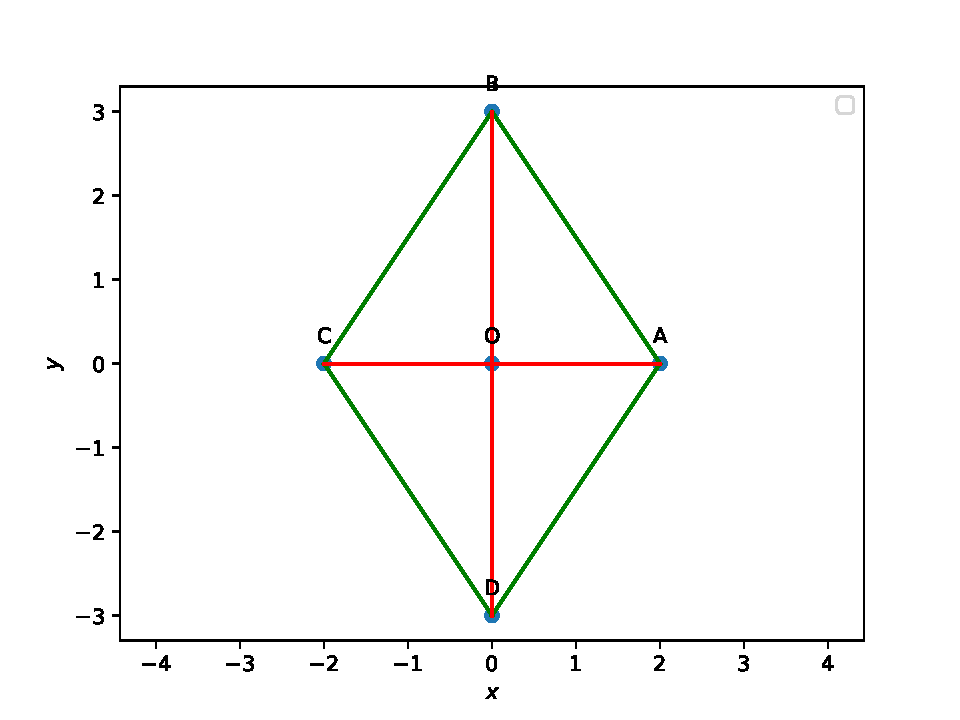
\includegraphics[width=\columnwidth]{chapters/9/8/1/7/figs/fig5.pdf} 
		\caption{}
		\label{fig:9/8/1/7}
  	\end{figure}
\begin{align}
		\label{eq:9/8/1/7}
		\begin{split}
	\norm{\vec{A}-\vec{B}}&=\norm{\vec{A}-\vec{D}}
\\
	\vec{A}-\vec{B}&=\vec{D}-\vec{C}
		\end{split}
\end{align}
From 
    \eqref{eq:angle2d},
\begin{align}
		\begin{split}
	\cos \angle{BAC}
	&= \frac{(\vec{A}-\vec{B})^T(\vec{A}-\vec{C})}{\norm{\vec{A}-\vec{B}}\norm{\vec{A}-\vec{C}}}
	\\
\cos	\angle{DAC}
	 &= \frac{(\vec{C}-\vec{D})^T(\vec{C}-\vec{A})}{\norm{\vec{C}-\vec{D}}\norm{\vec{C}-\vec{A}}}
		\end{split}
	 \label{eq:9/8/1/8/cang}
%
\end{align}
From 
		\eqref{eq:9/8/1/7}
and
	 \eqref{eq:9/8/1/8/cang}, 
%
	 we obtain
\begin{align}
		\begin{split}
	\cos \angle{BAC}
	=\cos \angle{DAC}
		\end{split}
\end{align}
Thus, $AC$ bisects $\angle A$.  Similarly, the remaining results can be proved.

\item 
\item 
\iffalse
\def\mytitle{PYTHON PROGRAMMING ON MATRICES}
\def\myauthor{K.Pavan Kumar}
\def\contact{r170850@rguktrkv.ac.in}
\def\mymodule{Future Wireless Communication (FWC)}
\documentclass[10pt, a4paper]{article}
\usepackage[a4paper,outer=1.5cm,inner=1.5cm,top=1.75cm,bottom=1.5cm]{geometry}
\twocolumn
\usepackage{graphicx}
\graphicspath{{./images/}}
\usepackage[colorlinks,linkcolor={black},citecolor={blue!80!black},urlcolor={blue!80!black}]{hyperref}
\usepackage[parfill]{parskip}
\usepackage{lmodern}
\usepackage{tikz}
	\usepackage{physics}
\usepackage{tabularx}
\usepackage{enumitem}
\usetikzlibrary{calc}
\usepackage{amsmath}
\usepackage{amssymb}
\renewcommand*\familydefault{\sfdefault}
\usepackage{watermark}
\usepackage{lipsum}
\usepackage{xcolor}
\usepackage{listings}
\usepackage{float}
\usepackage{titlesec}
\providecommand{\mtx}[1]{\mathbf{#1}}
\titlespacing{\subsection}{1pt}{\parskip}{3pt}
\titlespacing{\subsubsection}{0pt}{\parskip}{-\parskip}
\titlespacing{\paragraph}{0pt}{\parskip}{\parskip}


\newcommand{\myvec}[1]{\ensuremath{\begin{pmatrix}#1\end{pmatrix}}}
\let\vec\mathbf
\lstset{
frame=single, 
breaklines=true,
columns=fullflexible
}
\thiswatermark{\centering \put(0,-110.0){
\includegraphics[scale=0.3]{logo.png}} }
\title{\mytitle}
\author{\myauthor\hspace{1em}\\\contact\\FWC22011\hspace{6.5em}IITH\hspace{0.5em}\mymodule\hspace{6em}Matrix:Line}
\date{}
\begin{document}
	\maketitle
	\tableofcontents
	\fi

In parallelogram $ABCD$, two points $\vec{P}$ and $\vec{Q}$ are
taken on diagonal $BD$ such that $DP = BQ$. Show that 
\begin{enumerate}
	\item  $\Delta APD \cong \Delta CQB$         
	\item  $AP = CQ$
	\item $\Delta AQB \cong \Delta CPD$     
	\item  $AQ = CP$   
	\item  $APCQ$ is a parallelogram 
\end{enumerate}
\solution 
See Fig. 
		\ref{fig:9/8/1/9}.
 	\begin{figure}
		\centering
 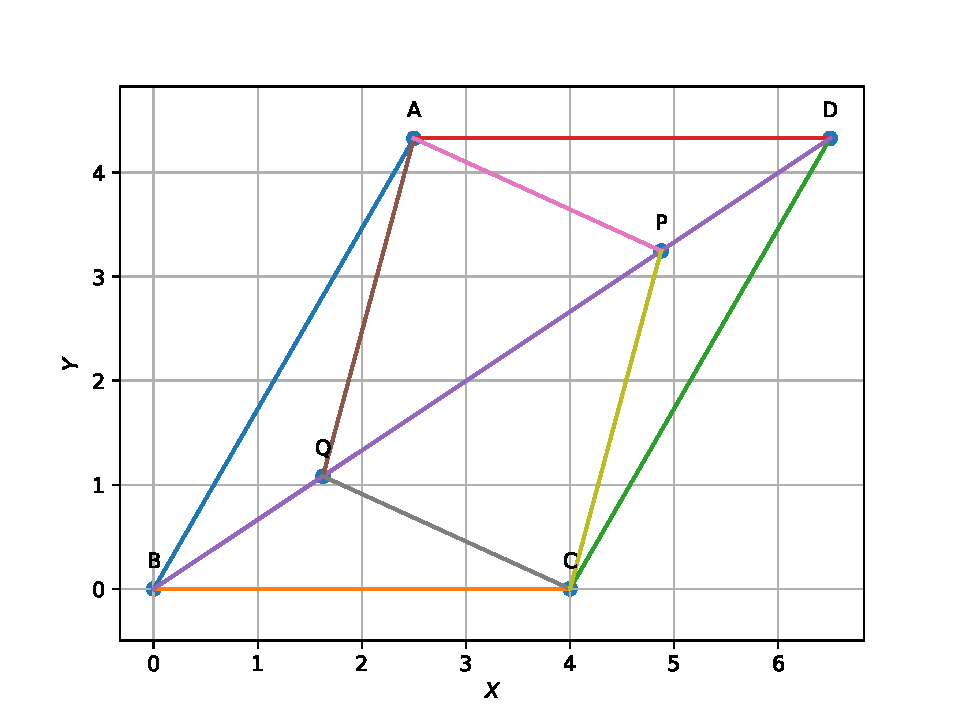
\includegraphics[width=\columnwidth]{chapters/9/8/1/9/figs/output.pdf}
		\caption{}
		\label{fig:9/8/1/9}
  	\end{figure}

\iffalse

\section{Construction}
  	\begin{center}
  Figure of construction
  	\end{center}

   
  \section{Solution}
\begin{center}
The input parameters for this construction are
\begin{tabular}{|c|c|}
	\hline
	\textbf{Symbol}&\textbf{Value}\\
	\hline
	r&5\\
	\hline
	k&3\\
	\hline
    b&4\\
	\hline
	$\theta$&$\frac{pi}{3}$\\
	\hline
\end{tabular}
\end{center}

\begin{align*}
\vec{A}=\begin{pmatrix} r\cos\theta\\ r\sin\theta\ \end{pmatrix} \\
\vec{B}=\begin{pmatrix} 0\\ 0\ \end{pmatrix} \\
\vec{C}=\begin{pmatrix} b\\ 0\ \end{pmatrix} \\
\vec{D}={\vec{A}+\vec{C}-\vec{B}} \\
\vec{P} =  \frac{\vec{B} +K\times \vec{D}}{1+K} \\
\vec{Q} =  \frac{K\times\vec{B} +\vec{D}}{1+K} \\ 
\end{align*}


\textbf{Theorem}\\
A quadrilateral is a parallelogram if a pair of opposite sides
is equal and parallel.

"If two directional vectors are equal,implies their magnitude as well as direction are equal to each other."

Two vectors are parallel if they have the same direction (or) are in exactly opposite directions.

\paragraph{Given} ABCD is a parallelogram.
 ,the two points $\vec{P}$ and $\vec{Q}$ are taken on diagonal BD such that DP = BQ.

\fi
From 
    \eqref{eq:angle2d} and the given information,

\begin{align}
	\vec{A}-\vec{B} &=\vec{D}-\vec{C} \\
	\implies    \vec{A}-\vec{D} &=\vec{B}-\vec{C}\\
	\vec{B}-\vec{Q} &=\vec{P}-\vec{D}
\end{align}

From (1) and (3):
\begin{align}
\begin{split}
    \vec{A}+\vec{C} =\vec{B}+\vec{D}\\
    \vec{P}+\vec{Q} =\vec{B}+\vec{D}
\end{split}
\end{align}

From (4)
\begin{align}
    \vec{A}+\vec{C} =\vec{P}+\vec{Q}
\end{align}

From (5)
\begin{align}
     \implies  \vec{A}-\vec{Q} =\vec{P}-\vec{C}\\
    \vec{A}-\vec{P} =\vec{Q}-\vec{C}
\end{align}


\begin{enumerate}
    \item From (2),(3) and (7)
    \begin{align}
        \Delta APD \cong \Delta CQB
    \end{align}
    
    \item \begin{align}
        Equation (7) \implies AP=CQ
    \end{align}
    
     \item From (1),(3) and (6)
    \begin{align}
        \Delta AQB \cong \Delta CPD
    \end{align}

    \item \begin{align}
        Equation (6) \implies AQ=CP
    \end{align}

     \item Equation (6) and (7) 
      $\implies$  Quadrilateral APCQ is a parallelogram.
\end{enumerate}

\iffalse

\textbf{termux commands :}
\begin{lstlisting}
bash lines.sh............using shell command
\end{lstlisting}
\begin{center}
Below python code realizes the above construction :
\fbox{\parbox{8.5cm}{\url{https://github.com/pavan170850/Fwciith2022/blob/main/matrices/line/code/Line.py}}}
\end{center}
\end{document}
\fi

\item 
\def\mytitle{PARALLELOGRAM}
\def\myauthor{VUNNAVA SRAVANI}
\def\contact{sravani21vunnava@gmail.com}
\def\mymodule{Future Wireless Communication (FWC)}
\documentclass[10pt, a4paper]{article}
\usepackage[a4paper,outer=1.5cm,inner=1.5cm,top=1.75cm,bottom=1.5cm]{geometry}
\twocolumn
\usepackage{setspace}
\doublespacing
\usepackage{graphicx}
\graphicspath{{./images/}}
\usepackage[colorlinks,linkcolor={black},citecolor={blue!80!black},urlcolor={blue!80!black}]{hyperref}
\usepackage[parfill]{parskip}
\usepackage{lmodern}
\usepackage{tikz}
	\usepackage{physics}
%\documentclass[tikz, border=2mm]{standalone}
\usepackage{karnaugh-map}
%\documentclass{article}
\usepackage{tabularx}
\usepackage{circuitikz}
\usetikzlibrary{calc}
\usepackage{amsmath}
\usepackage{amssymb}
\renewcommand*\familydefault{\sfdefault}
\usepackage{watermark}
\usepackage{lipsum}
\usepackage{xcolor}
\usepackage{listings}
\usepackage{float}
\usepackage{titlesec}
\providecommand{\mtx}[1]{\mathbf{#1}}
\titlespacing{\subsection}{1pt}{\parskip}{3pt}
\titlespacing{\subsubsection}{0pt}{\parskip}{-\parskip}
\titlespacing{\paragraph}{0pt}{\parskip}{\parskip}
\newcommand{\figuremacro}[5]{
    \begin{figure}[#1]
        \centering
        \includegraphics[width=#5\columnwidth]{#2}
        \caption[#3]{\textbf{#3}#4}
        \label{fig:#2}
    \end{figure}
}
\newcommand{\myvec}[1]{\ensuremath{\begin{pmatrix}#1\end{pmatrix}}}
\let\vec\mathbf
\lstset{
frame=single, 
breaklines=true,
columns=fullflexible
}

%\thiswatermark{\centering \put(181,-119.0){\includegraphics[scale=0.13]{IIT_logo.png}} }
\title{\mytitle}
\author{\myauthor\hspace{1em}\\\contact\\FWC22012\hspace{6.5em}IITH\hspace{0.5em}\mymodule\hspace{6em}ASSIGN-5}
\date{}
\begin{document}
	\maketitle
	\tableofcontents
   \section{Problem}
  ABCD is a parallelogram and AP and CQ are
perpendiculars from vertices A and C on diagonal
BD . Show that \\
(i) $\Delta APB \cong \Delta CQD$  \\       
(ii) AP = CQ

	   % 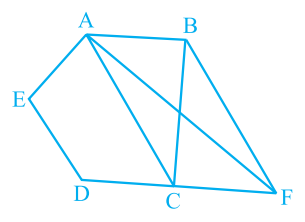
\includegraphics[scale=1.0]{diag_1.png}
   \section{Solution}

The input parameters for this construction are 
\begin{center}
\begin{tabular}{|c|c|}
	\hline
	\textbf{Symbol}&\textbf{Value}\\
	\hline
	b&6\\
	\hline
	r&5\\
	\hline
	$\theta$&$\frac{\pi}{3}$\\
	\hline
\end{tabular}
\begin{center}
$\vec{A}=\myvec{0\\0}$\\
$\vec{D}=\myvec{r\cos\theta \\ r\sin\theta}$\\
$\vec{B}=\myvec{0\\b}$\\
$\vec{C} = \vec{B}+\vec{C}$
\end{center}
\end{center}
\textbf{To Prove:} AP = CQ
		\begin{center}
		The line equation for diagonal BD is $x = \vec{B}+\lambda\vec{m}$
		\\
		where $\vec{m} = \vec{B}-\vec{D}$\\
		
		then,\\
		
		$\vec{P} = \vec{B} - \frac{\vec{m}^T \vec{B}}{\norm{\vec{m}}^2}\vec{m}$
	\\
	
	$\vec{Q} = \vec{B} - \frac{\vec{m}^T \vec{B-C}}{\norm{\vec{m}}^2}\vec{m}$\\
	\end{center}
	
	distance between A and P is $\norm{\vec{A-P}}$\\
	distance between C and Q is $\norm{\vec{C-Q}}$\\
	if $\norm{\vec{A-P}}$ =  $\norm{\vec{C-Q}}$\\
	then AP = CQ..........(1)
	
	\textbf{To Prove:}  $\Delta APB \cong \Delta$ CQD\\
	to prove $\angle {APD}=\angle {CQD}=90^{\circ}$\\
	$\vec{m1} = \vec{A-P}$\\
	$\vec{m2} = \vec{P-B}$\\
	$\theta= \angle {APD}$ \\
	 $\cos\theta$ = $\frac{\vec{m1}^T \vec{m2}}{\norm{\vec{m1}}\norm{\vec{m2}}}$\\
	$\theta = 90^{\circ}, cos\theta$ = 0\\
	$\therefore m1^T m2 = 0$\\
	$\vec{n1} = \vec{C-Q}$\\
	$\vec{n2} = \vec{Q-D}$\\
	$\theta = \angle{CQD}$\\
	$cos\theta$ = $\frac{\vec{n1}^T \vec{n2}}{\norm{\vec{n1}}\norm{\vec{n2}}}$\\
	f $\theta$ = 90$^{\circ}, cos\theta$ = 0\\
	$\therefore n1^T n2 = 0$\\
	\begin{center}
	if 	$m1^T m2 = n1^T n2$ = 0\\
	then, $\angle {APD} = \angle {CQD} = 90^{\circ}$..........(2)\\
	\end{center}
	to prove $\angle {ABP}=\angle {CDQ}$ \\
	$\vec{m2} = \vec{P-B}$\\
	$\vec{m3} = \vec{A-B}$\\
	$\theta1 = \angle {ABP}$\\
	$\theta1 = \cos^-1\frac{\vec{m2} \cdot \vec{m3}}{\norm{\vec{m2}}\norm{\vec{m3}}}$\\
	$\vec{n2} = \vec{C-D}$\\
	$\vec{n3} = \vec{Q-D}$\\
	$\theta2 = \angle {CDQ}$\\
	$\theta2 = \cos^-1\frac{\vec{n2} \cdot \vec{n3}}{\norm{\vec{n2}}\norm{\vec{n3}}}$\\
	\begin{center}
	 		if $\theta1 = \theta2$\\
	 		then $\angle {ABP} = \angle {CQD}$..........(3)
	\end{center}
	\begin{center}
$\therefore$ from (1),(2) and (3)
$\Delta APB \cong \Delta CQD$ 
	\end{center}
The below python code realizes the above construction:	\\
\begin{lstlisting}
https://github.com/sravani21vunnava/sravani21vunnava/blob/main/Matrices_line/codes/matrix_line.py
\end{lstlisting}
 
\section{Construction}
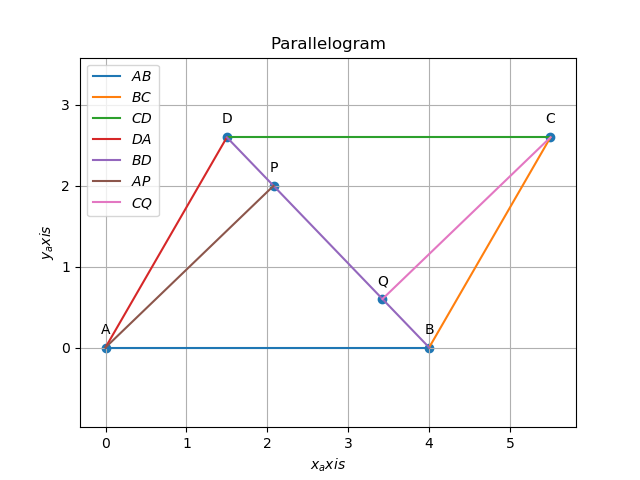
\includegraphics[scale=0.66]{matrix_line.png}
 	
\bibliographystyle{ieeetr}
\end{document}
\item 

\documentclass[10pt, a4paper]{article}
\usepackage[a4paper,outer=1.5cm,inner=1.5cm,top=1.75cm,bottom=1.5cm]{geometry}

\twocolumn
\usepackage{graphicx}
\usepackage{karnaugh-map}
\usepackage{tabularx}
\usepackage{hyperref}
\usepackage[utf8]{inputenc}
\usepackage{amsmath}
\usepackage{physics}
\usepackage{amssymb}

\begin{document}
\title{Assignment-4}
\author{Name:A.Gowri Priya\and Email :  \url{gowripriyaappayyagari@gmail.com}}
%\{ Wireless Communication (FWC)}
\date{}
\maketitle


  \section{Problem}
In  $\Delta$  ABC and  $\Delta$ DEF, AB = DE, AB $\parallel$ DE, BC = EF
and BC $\parallel$ EF. Vertices A, B and C are joined to
vertices D, E and F respectively (see Figure).\\
Show that\\
(i) quadrilateral ABED is a parallelogram\\
(ii) quadrilateral BEFC is a parallelogram\\
(iii) AD $\parallel$ CF and AD = CF\\
(iv) quadrilateral ACFD is a parallelogram\\
(v) AC = DF\\
(vi)$\Delta ABC \cong \Delta$  DEF.\\
\begin{figure}[h]
\centering
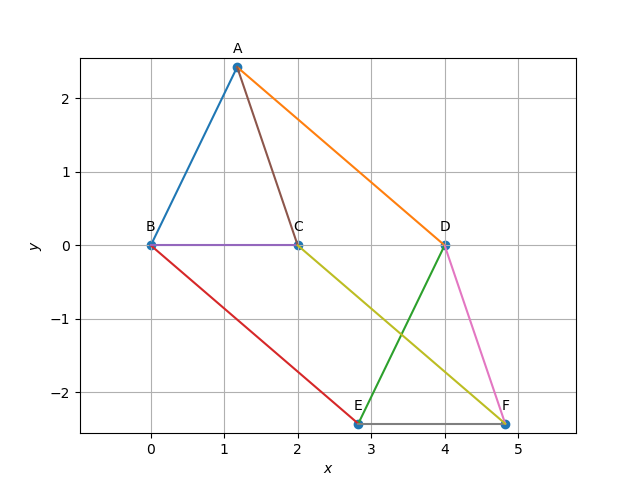
\includegraphics[scale=0.5]{fig.png} 
\caption{Given Figure}
\end{figure}

\section{Solution}
\begin{center}
The input parameters for this construction are
\begin{tabular}{|c|c|}
	\hline
	\textbf{Symbol}&\textbf{Value}\\
	\hline
	r1&2\\
	\hline
	r2&3\\
	\hline
	$\theta$&$\frac{{3}\pi}{10}$\\
	\hline
\end{tabular}
\boldmath
$$\vec{A}=\begin{pmatrix} r1\cos\theta\\ r2\sin\theta\ \end{pmatrix}$$
$$\vec{B}=\begin{pmatrix} 0\\ 0\ \end{pmatrix}$$
$$\vec{D}=\begin{pmatrix} 4\\ 0\ \end{pmatrix}$$
$$\vec{C}={\vec{B}+\vec{D}}/2$$
$$\vec{E}={\vec{B}+\vec{D}-\vec{A}}$$
$$\vec{F}={\vec{E}+\vec{C}-\vec{B}}$$
\unboldmath
\end{center}
\textbf{Direction vectors}

The Direction vectors are
\boldmath
$$\vec{m_1}={\vec{A}-\vec{B}} $$
$$\vec{m_2}={\vec{B}-\vec{C}} $$
$$\vec{m_3}={\vec{C}-\vec{A}} $$
$$\vec{n_1}={\vec{D}-\vec{E}} $$
$$\vec{n_2}={\vec{E}-\vec{F}} $$
$$\vec{n_3}={\vec{F}-\vec{D}} $$
$$\vec{o_1}={\vec{A}-\vec{D}} $$
$$\vec{o_2}={\vec{C}-\vec{F}} $$
\unboldmath
\textbf{To proove\\ i.Quadrilateral ABED is a parallelogram}\\
    Distance between A and B is $\norm{\vec{A-B}}$\\
	Distance between D and E is $\norm{\vec{D-E}}$\\
	if $\norm{\vec{A-B}}$ =  $\norm{\vec{D-E}}$\\
	then AB = DE..........(1)\\
	if $\vec{m_1} \times \vec{n_1}=0$\\
	then AB $\parallel$ DE...........(2)\\
	Because,Two vectors ara parallel when cross product of that two vectors is zero.\\
	From (1) and (2) we can say that ABED is a parallelogram.Because,If one pair of opposite sides of a quadrilateral are equal and parallel to each other,then it is a parallelogram.\\
	$\therefore$ Quadrilateral ABED is a parallelogram.\\ 
\textbf{ii.Quadrilateral BEFC is a parallelogram}\\
    Distance between B and C is $\norm{\vec{B-C}}$\\
	Distance between E and F is $\norm{\vec{E-F}}$\\
	if $\norm{\vec{B-C}}$ =  $\norm{\vec{E-F}}$\\
	then BC = EF..........(3)\\
	if $\vec{m_2} \times \vec{n_2}=0$\\
	then BC $\parallel$ EF...........(4)\\
	Because,Two vectors ara parallel when cross product of that two vectors is zero.\\
	From (3) and (4) we can say that BEFC is a parallelogram.Because,If one pair of opposite sides of a quadrilateral are equal and parallel to each other,then it is a parallelogram.\\
	$\therefore$ Quadrilateral BEFC is a parallelogram.\\ 	
\textbf{iii.AD$\parallel$CF and AD=CF}\\
    Distance between A and D is $\norm{\vec{A-D}}$\\
	Distance between C and F is $\norm{\vec{C-F}}$\\
	if $\norm{\vec{A-D}}$ =  $\norm{\vec{C-F}}$\\
	then AD = CF..........(5)\\
	if $\vec{O_1} \times \vec{O_2}=0$\\
	then AD $\parallel$ CF...........(6)\\
	Because,Two vectors ara parallel when cross product of that two vectors is zero.\\
	From (5) and (6) AD$\parallel$CF and AD=CF \\
\textbf{iv.Quadrilateral ACFD is a parallelogram}\\
   From (iii) we can say that AD$\parallel$CF and AD=CF 
	SO, we can say that ACFD is a parallelogram.Because,If one pair of opposite sides of a quadrilateral are equal and parallel to each other,then it is a parallelogram.\\
	$\therefore$ Quadrilateral ACFD is a parallelogram.\\
\textbf{v.AC=DF}\\
    Distance between A and C is $\norm{\vec{A-C}}$\\
	Distance between D and F is $\norm{\vec{D-F}}$\\
	if $\norm{\vec{A-C}}$ =  $\norm{\vec{D-F}}$\\
	then AC = DF\\
	$\therefore$ AC=DF\\
\textbf{vi.$\Delta ABC \cong \Delta DEF$}  \\
If $\norm{\vec{A-B}}$ =  $\norm{\vec{D-E}}$ and $\norm{\vec{B-C}}$ =  $\norm{\vec{E-F}}$ and $\norm{\vec{A-C}}$ =  $\norm{\vec{D-F}}$\\
Then,$\Delta ABC \cong \Delta DEF$ .Because, If three sides of one triangle are equal to three sides of another triangle, the triangles are congruent.(By SSS Rule)\\
$\therefore$ $\Delta ABC \cong \Delta DEF$

\section{Execution}
*Verify the above proofs in the following code.\\
\framebox{
\url{https://github.com/gowripriya-2002/FWC/blob/main/line_assignment/line.py}}	
\bibliographystyle{ieeetr}
\end{document}

\item 
\iffalse
\documentclass[journal,10pt,twocolumn]{article}
\usepackage[margin=0.5in]{geometry}
\usepackage[cmex10]{amsmath}
\usepackage{array}
\usepackage{booktabs}

% The preceding line is only needed to identify funding in the first footnote. If that is unneeded, please comment it out.
\usepackage{cite}
\usepackage{amsmath,amssymb,amsfonts}
\usepackage{graphicx}
\usepackage{textcomp}
\usepackage{xcolor}
\usepackage{graphicx}
\graphicspath{{./fig}}{}
\def\BibTeX{{\rm B\kern-.05em{\sc i\kern-.025em b}\kern-.08em
    T\kern-.1667em\lower.7ex\hbox{E}\kern-.125emX}}

\usepackage{tikz}
\usetikzlibrary{shapes.geometric}
\usetikzlibrary{shapes.geometric,angles,quotes}


\begin{document}



\newtheorem{theorem}{Theorem}[section]
\newtheorem{problem}{Problem}
\newtheorem{proposition}{Proposition}[section]
\newtheorem{lemma}{Lemma}[section]
\newtheorem{corollary}[theorem]{Corollary}
\newtheorem{example}{Example}[section]
\newtheorem{definition}[problem]{Definition}
%\newtheorem{thm}{Theorem}[section] 
%\newtheorem{defn}[thm]{Definition}
%\newtheorem{algorithm}{Algorithm}[section]
%\newtheorem{cor}{Corollary}
\newcommand{\BEQA}{\begin{eqnarray}}
\newcommand{\EEQA}{\end{eqnarray}}
\newcommand{\define}{\stackrel{\triangle}{=}}
\newcommand*\circled[1]{\tikz[baseline=(char.base)]{
    \node[shape=circle,draw,inner sep=2pt] (char) {#1};}}

\bibliographystyle{article}
%\bibliographystyle{ieeetr}


\providecommand{\mbf}{\mathbf}
\providecommand{\pr}[1]{\ensuremath{\Pr\left(#1\right)}}
\providecommand{\re}[1]{\ensuremath{\text{Re}\left(#1\right)}}
\providecommand{\im}[1]{\ensuremath{\text{Im}\left(#1\right)}}
\providecommand{\qfunc}[1]{\ensuremath{Q\left(#1\right)}}
\providecommand{\sbrak}[1]{\ensuremath{{}\left[#1\right]}}
\providecommand{\lsbrak}[1]{\ensuremath{{}\left[#1\right.}}
\providecommand{\rsbrak}[1]{\ensuremath{{}\left.#1\right]}}
\providecommand{\brak}[1]{\ensuremath{\left(#1\right)}}
\providecommand{\lbrak}[1]{\ensuremath{\left(#1\right.}}
\providecommand{\rbrak}[1]{\ensuremath{\left.#1\right)}}
\providecommand{\cbrak}[1]{\ensuremath{\left\{#1\right\}}}
\providecommand{\lcbrak}[1]{\ensuremath{\left\{#1\right.}}
\providecommand{\rcbrak}[1]{\ensuremath{\left.#1\right\}}}

\newcommand{\sgn}{\mathop{\mathrm{sgn}}}

%\providecommand{\hilbert}{\overset{\mathcal{H}}{ \rightleftharpoons}}
\providecommand{\system}{\overset{\mathcal{H}}{ \longleftrightarrow}}
	%\newcommand{\solution}[2]{\textbf{Solution:}{#1}}
\newcommand{\solution}{\noindent \textbf{Solution: }}
\newcommand{\cosec}{\,\text{cosec}\,}
\providecommand{\dec}[2]{\ensuremath{\overset{#1}{\underset{#2}{\gtrless}}}}
\newcommand{\myvec}[1]{\ensuremath{\begin{pmatrix}#1\end{pmatrix}}}
\newcommand{\mydet}[1]{\ensuremath{\begin{vmatrix}#1\end{vmatrix}}}
	\newcommand*{\permcomb}[4][0mu]{{{}^{#3}\mkern#1#2_{#4}}}
\newcommand*{\perm}[1][-3mu]{\permcomb[#1]{P}}
\newcommand*{\comb}[1][-1mu]{\permcomb[#1]{C}}

%\numberwithin{align}{section}
\numberwithin{align}{subsection}
%\numberwithin{problem}{section}
%\numberwithin{definition}{section}

\let\vec\mathbf




\title{
{Comparision of Angles and Sides of Trapezium\\
Using Matrices and lines}\\

\thanks{Meer Tabres Ali as an intern with FWC IIT Hyderabad. *The author is with the Department of Electrical Engineering, Indian Institute of Technology, Hyderabad 502285 India e-mail: gadepall@iith.ac.in. All content in this manual is released under GNU GPL. Free and open source.}
}
\author{Meer Tabres Ali and G V V Sharma}
\maketitle
\tableofcontents
\section{Problem statement}
\fi
$ABCD$ is trapezium in which $AB \parallel CD$ and $AD=BC$.
Show that, 
\begin{enumerate}
    \item $\angle A = \angle B$
    \item $\angle C = \angle D$
    \item Diagonal $AC$ = Diagonal $BD$
    \item $\triangle ABC  = \triangle BAD$
\end{enumerate}
\iffalse
\solution 
See Fig. 
		\ref{fig:9/8/1/12}.
	\begin{figure}[!h]
		\centering
 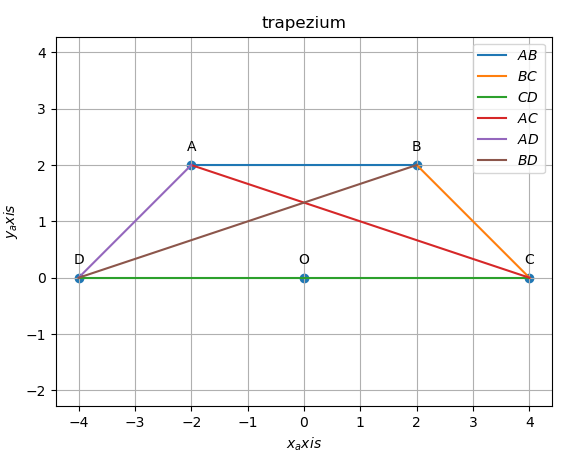
\includegraphics[width=\columnwidth]{chapters/9/8/1/12/figs/trapezium1.png}
		\caption{}
		\label{fig:9/8/1/12}
  	\end{figure}
For $\vec{e}_1$ defined in Appedix \ref{def:matrix-two},
    Let 
\begin{align}
	 \label{eq:9/8/1/12/cang}
		\begin{split}
	\vec{D} &= \vec{0}
	\\
	\vec{C}&= c\vec{e}_1
\\
	\vec{A}&= r\myvec{\cos D \\ \sin D}
\\
	\vec{B}&= \vec{C} +  r\myvec{-\cos C \\ \sin C}
		\end{split}
\end{align}
%
Thus, 
\begin{align}
	 \label{eq:9/8/1/12/cang/a}
	\cos \angle{BAD}
	&= \frac{(\vec{A}-\vec{B})^T(\vec{A}-\vec{D})}{\norm{\vec{A}-\vec{B}}\norm{\vec{A}-\vec{D}}}
	\\
\cos	\angle{CBA}
	 &= \frac{(\vec{B}-\vec{C})^T(\vec{B}-\vec{A})}{\norm{\vec{B}-\vec{C}}\norm{\vec{B}-\vec{A}}}
	 \label{eq:9/8/1/12/cang/b}
%
\end{align}
Substituting from 
	 \eqref{eq:9/8/1/12/cang},
\begin{align}
	 \label{eq:9/8/1/12/cang/abd}
	 (\vec{A}-\vec{B})^T(\vec{A}-\vec{D}) &= r\brak{r\myvec{\cos D+ \cos C  & \sin D - \sin C}-c\vec{e}_1^{\top}}\myvec{\cos D \\ \sin D}
	 \\
	&= r\brak{r\brak{1+ \cos \brak{C+D}  }-c\cos D }
\end{align}
Similarly, 
\begin{align}
	 \label{eq:9/8/1/12/cang/abc}
(\vec{B}-\vec{C})^T(\vec{B}-\vec{A})
	&= r\brak{-r\myvec{\cos D+ \cos C  & \sin D - \sin C}+c\vec{e}_1^{\top}}\myvec{-\cos C \\ \sin C}
	 \\
	&= r\brak{r\brak{1+ \cos \brak{C+D}  }-c\cos D }
\end{align}

	 \eqref{eq:9/8/1/12/cang},
\section{Considerations}
\vspace{0.2cm}
The input parameters are the lengths r, c and angle $\theta$. \\
\vspace{0.2cm}
{


\setlength\extrarowheight{2pt}
\begin{tabular}{|c|c|c|}
	\hline
	\textbf{Symbol}&\textbf{Value}&\textbf{Description}\\
	\hline
	$\vec{O}$ & \myvec{0\\0}
	&Origin\\
	\hline
	r&2.82& Distance of BC, AD\\
	\hline
	c&4&OC\\
	
	\hline
	$\vec{C}$ & \myvec{c \\ 0}

	&Point C on X axes
	\\
\hline
	$\theta$&45 \textdegree &$\angle$BOC\\
	\hline
\end{tabular}
}


\section{Plotting Trapezium}




\vspace{0.25cm}
Plot of Trapezium is shown in figure 1, where point O is origin and points A, B, C and D are the vertices of Trapezium.
\begin{figure}[h]

\caption{trapezium}
\label{fig:trapezium}
\end{figure}


\section{Solution}

\vspace{0.25cm}
\subsection{Finding Co-ordinates O, A, B, C and D}
\begin{flushleft}
Let O be the origin and its coordinates are\\
\vspace{0.25cm}

\center
\vspace{0.4cm}
$\vec{O}$ = \myvec{0\\0}
\endcenter{}
\vspace{0.25cm}
Let C be the point on X-axes and it is expressed as\\
\vspace{0.25cm}
\begin{align}
    \vec{C} = c
    \end{align}

\vspace{0.25cm}
\begin{flushleft}
Let D be the point on Negative X-axes and it will be the image of C,\\
\begin{center}
$\vec{D}$  = -c\\
\end{center}
\vspace{0.2cm}
Therefore, the coordinates of D are\\
\end{flushleft}


\vspace{0.25cm}
\begin{flushleft}
Let r be the distance between point B and C, then\\
\end{flushleft}

\vspace{0.25cm}
$|| \vec{B-C} || $ = r and $|| \vec{A-D} || $ = r\\
\vspace{0.25cm}
\begin{flushleft}
Let $\theta$ be the angle at BOC, then\\
\end{flushleft}
\vspace{0.25cm}
$\angle$BOC = $\theta$\\
\vspace{0.25cm}
\begin{flushleft}
According to the vector geometry formulaes, the vector B can be expresssed as\\
\end{flushleft}
\vspace{0.25cm}
\begin{align}
   \vec{B}= r \myvec{cos\theta \\ sin\theta}
\end{align}

\vspace{0.35cm}
\begin{flushleft}
From ABCD trapezium, \\
\end{flushleft}
\begin{center}
$\vec{A} =\vec{B}-  \vec{C}$\\
\end{center}

\center
\vspace{0.4cm}
= \myvec{rcos $$\theta$$ \\ rsin $$\theta$$} - \myvec{c \\ 0}
   
\endcenter{}
		= \myvec{-c+rcos $$ \theta$$ \\ rsin$$\theta$$}
	\\
\vspace{0.3cm}
\begin{flushleft}
From triangle ODA,
$\boldsymbol{OD+DA=OA}$, \\
\vspace{0.2cm} 
$\implies$ -c+rcos$\theta$ = -r cos $\theta$\\
\end{flushleft}
\vspace{0.35cm}
	= \myvec{-rcos $$ \theta$$ \\ rsin$$\theta$$} \\
\endcenter{}
	$\implies$ $\vec{A}$
	= r\myvec{-cos $$ \theta$$ \\ sin$$\theta$$} \\

Let c=4, r=2.82 and $\theta$=45 \textdegree \\

Then all the four coordinates will be, \\

\vspace{0.3cm}
$\vec{O}$=\myvec{0 \\ 0}, $\vec{A}$=\myvec{-2 \\ 2}, $\vec{B}$=\myvec{2 \\ 2}, $\vec{C}$=\myvec{4 \\ 0}, $\vec{D}$=\myvec{-4 \\ 0}
\\

\subsection{Calculation of Angles A and B}
\vspace{0.25cm}
To find angle $\angle$A:\\

\begin{center}
    

$\vec{A-D}$ = \myvec{-2 \\ 2} - \myvec{-4 \\ 0}
	= \myvec{2 \\ 2}

\begin{flushleft}
and \\
\end{flushleft}


$\vec{A-B}$ = \myvec{-2 \\ 2} -\myvec{2 \\ 2} = \myvec{-4 \\ 0}
	\\

\end{center}
\vspace{0.4cm}
\begin{align}
\angle BAD = arccos \vec{\frac{(A-D).(A-B)}{||A-D ||. ||A-B||}}
\end{align}
\vspace{0.4cm}
\begin{align}
\angle BAD = arccos \frac{(2 \hspace{0.32cm}  2)^T . (-4 \hspace{0.25cm}   0) } {\sqrt{2^2+2^2}.\sqrt{4^2+0}}
\end{align}

\begin{align}
= arccos \frac{-8 } {\sqrt{8}.\sqrt{16}} = arccos (-0.707) 
\end{align}
\begin{flushleft}
$\implies$   $\angle$ BAD = 135 \textdegree\\
\vspace{0.3cm}
$\implies$   $\angle$ A = 135 \textdegree
\end{flushleft}

\vspace{0.5cm}
\begin{flushleft}
To find angle $\angle$ B: \\
\end{flushleft}

\vspace{0.35cm}
$\vec{B-A}$ = \myvec{2 \\ 2}-\myvec{-2 \\ 2}
	= \myvec{4\\0}
and \\

$\vec{B-C}$ = \myvec{2 \\ 2} -\myvec{4\\0} = \myvec{-2 \\2} 
\vspace{0.25cm}	
\begin{align}
\angle BAD = arccos \vec {\frac{(A-D).(A-B)}{||A-D||.||A-B||}}
\end{align}

\begin{align}
\angle BAD = arccos \frac{(4, 0)^T .(-2, 2)}{\sqrt{4^2}.\sqrt{2^2+2^2} }
\end{align}

\begin{align}
= arccos \frac{-8 } {\sqrt{16}.\sqrt{8}} =arccos (-0.707)
\end{align}

\begin{flushleft}
$\implies$   $\angle$ ABC = 135 \textdegree\\
\vspace{0.3cm}
$\implies$   $\angle$ B = 135 \textdegree
\\
\vspace{0.3cm}
Therefore $\angle A$ = $\angle B$
\end{flushleft}

\subsection{Calculation of Angles C and D}
\vspace{0.25cm}

To find angle $\angle$C:\\
$\vec{C-O}$ = \myvec{4\\0} - \myvec{0\\0}
	= \myvec{4\\0}
and 

$\vec{C-B}$ = \myvec{4\\0}- \myvec{2\\2} = \myvec{2\\-2}
\\

\begin{align}
\angle OCB = arccos \vec{\frac{(C-O).(C-B)}{||C-O ||. ||C-B||}}
\end{align}

\begin{align}
\angle BAD = arccos \frac{(4 \hspace{0.15cm} 0)^T . (2 \hspace{0.15cm} -2) } {\sqrt{4^2}.\sqrt{2^2+2^2}}
\end{align}

\begin{align}
= arccos \frac{8 } {\sqrt{16}.\sqrt{8}} = arccos (0.707)
\end{align}
\begin{flushleft}
$\implies$   $\angle$ OCB = 45 \textdegree\\
\vspace{0.3cm}
$\implies$   $\angle$ C = 45 \textdegree
\end{flushleft}

\vspace{0.5cm}
\begin{flushleft}
To find angle $\angle$ D: \\
\end{flushleft}
\vspace{0.2cm}
\center
$\vec{D-O}$ = \myvec{-4\\0}-\myvec{0\\0}= \myvec{-4 \\ 0}
\\
\endcenter
\begin{flushleft}
and \\
\end{flushleft}


$\vec{D-A}$ = \myvec{-4 \\ 0} -\myvec{-2 \\ 2} = \myvec{-2 \\ -2}

\endcenter

\begin{align}
\angle ODB = arccos \vec{\frac{(D-O).(D-B)}{||D-O ||. ||D-B||}}
\end{align}

\begin{align}
\angle ODB = arccos \frac{(-4 \hspace{0.29cm} 0)^T .(-2 \hspace{0.22cm} -2)}{\sqrt{4^2}.\sqrt{2^2+2^2} }
\end{align}

\begin{align}
= arccos \frac{8} {\sqrt{8}.\sqrt{16}} = arccos (0.707)
\end{align}

\begin{flushleft}
$\implies$   $\angle$ ODB = 45 \textdegree\\
\vspace{0.3cm}
$\implies$   $\angle$ D = 45 \textdegree
\end{flushleft}

Therefore $\angle C$ = $\angle D$

\subsection{Calculation of Diagonals AC and BD}
\vspace{0.2cm}
\begin{flushleft}
Calculation of Diagonal AC:\\
\end{flushleft}

\vspace{0.1cm}

$\vec{A-C}$ = \myvec{-2 \\ 2} - \myvec{4 \\ 0} = \myvec{-6\\2}
	\\
\begin{flushleft}
Legth of Diagonal AC,\\
\end{flushleft}


$\vec{||A-C||}$ = $ || \myvec{-6 \\ 2} ||$
	\\
\vspace{0.25cm}
= $\sqrt{(-6)^2+2^2}$ = 6.32\\
\vspace{0.3cm}
$\implies$ $\vec{||A-C||}$=6.32\\

\vspace{0.3cm}
\begin{flushleft}
Calculation of Diagonal BD:\\
\end{flushleft}

\vspace{0.25cm}

$\vec{B-D}$ = \myvec{2\\2}- \myvec{-4\\0} = \myvec{6 \\ 2}
	\\
\begin{flushleft}
Length of Diagonal BD,\\
\end{flushleft}

$\vec{||B-D||}$ =  $||\myvec{6 \\2}||$
	\\
\vspace{0.25cm}
= $\sqrt{6^2+2^2}$ = 6.32\\
\vspace{0.25cm}
$\implies$ $\vec{||B-D||}$=6.32\\
\begin{flushleft}
Therefore both diagonals are equal,  AC = BD \\
\end{flushleft}

\subsection{Comparing $\triangle$ ABC and $\triangle$ BAD }
\begin{flushleft}
\vspace{0.25cm}
For Triangle ABC:\\
\vspace{0.25cm}
$\angle ABC = \angle AOC = \pi -\theta$ = 135 \textdegree \\
\vspace{0.25cm}
and\\
\vspace{0.25cm}
Base =Diagonal AC  = $\vec{||A-C||}$ = 6.32\\
\vspace{0.35cm}

For Triangle BAD:\\
\vspace{0.25cm}
$\angle BAD = \angle BOD = \pi -\theta$ = 135 \textdegree \\
\vspace{0.25cm}
and\\
\vspace{0.25cm}
Base =Diagonal AC  = $\vec{||B-D||} $ = 6.32\\
\vspace{0.35cm}
As base and opposite angles are same, both triangles are symmetrical.
\vspace{0.25cm}\\
Therefore  $\triangle$ ABC and $\triangle$ BAD
\end{flushleft}

\section{Software}
\centering
Download the codes given in the link below and execute them.\\
\begin{table}[h]
\centering
\begin{tabular}{|c|} \hline
\rule{0pt}{10pt} 
https://github.com/meertabresali-FWC-IITH/project/blob \\
/main/Asgn4.matrixline/line.py\\
\\\hline
 \end{tabular}
\end{table}
\section{Conclusion}
\begin{flushleft}
In this program, the following points have been verified.\\
\vspace{0.1cm}
\begin{enumerate}
    \item $\angle$ A = $\angle$ B\\
    \item $\angle$ C = $\angle$ D\\
    \item Diagonal AC = Diagonal BD\\
    \item $\triangle$ ABC  = $\triangle$ BAD \\
\end{enumerate}
\end{flushleft}
\end{document}
\fi



\fi


\end{enumerate}



%
\chapter{This is Chapter Two Title}

\section{This is First Level Heading}
\lipsum[1-2]

\subsection{This is Second Level Heading}
\lipsum[3]

\subsubsection{This is Third Level Heading}
\lipsum[4]

\paragraph{This is Fourth Level Heading}
\lipsum[5]

\subparagraph{This is Fifth Level Heading}
\lipsum[6] 
\backmatter
\appendix
\chapter{ Vectors}
\section{$2\times 1$ vectors}

\renewcommand{\theequation}{\theenumi}
%\begin{enumerate}[label=\arabic*.,ref=\theenumi]
\begin{enumerate}[label=\thesection.\arabic*.,ref=\thesection.\theenumi]
\numberwithin{equation}{enumi}
\item Let 
\begin{align}
  \vec{A} \equiv \overrightarrow{A} &= \myvec{a_1\\a_2} 
  \\
  &\equiv a_1\overrightarrow{i}+a_2\overrightarrow{j}, 
  \\
  \vec{B} &= \myvec{b_1\\b_2}, 
\end{align}
be $2 \times 1$ vectors.
Then, the determinant of the $2 \times 2$ matrix 
\begin{align}  
  \vec{M} = \myvec{\vec{A} & \vec{B}}
\end{align}
is defined as
\begin{align}
  \label{eq:det2d}
  \mydet{\vec{M}} &= \mydet{\vec{A} & \vec{B}} 
  \\
  &= \mydet{a_1 & b_1\\a_2 & b_2} = a_1b_2 - a_2 b_1
\end{align}
%
\item The value of the cross product of two vectors is given by  
  \eqref{eq:det2d}.
\item The area of the triangle with vertices $\vec{A}, \vec{B}, \vec{C}$ is given by the absolute value of 
\begin{align}
  \label{eq:area2d}
\frac{1}{2} \mydet{\vec{A-B} & \vec{A-C}}
  \end{align}
  \item  The transpose of $\vec{A}$ is defined as
\begin{align}
  \label{eq:transpose2d}
  \vec{A}^{\top}  = \myvec{a_1 & a_2}
\end{align}
%
\item The {\em inner product} or {\em dot product} is defined as
\begin{align}
  \label{eq:dot2d}
  \vec{A}^{\top} \vec{B} &\equiv \vec{A} \cdot \vec{B} 
  \\
  &= \myvec{a_1 & a_2} \myvec{b_1 \\ b_2}= a_1b_1+a_2b_2 
\end{align}
%
\item {\em norm} of $\vec{A}$ is defined as
\begin{align}
  \label{eq:norm2d}
  \norm{A} &\equiv \mydet{\overrightarrow{A}}
  \\
  &= \sqrt{\vec{A}^{\top} \vec{A}}= \sqrt{a_1^2+a_2^2}
\end{align}
Thus, 
\begin{align}
  \label{eq:norm2d_const}
  \norm{\lambda \vec{A}} &\equiv \mydet{\lambda\overrightarrow{A}}
  \\
  &= \abs{\lambda} \norm{\vec{A}}
\end{align}
\item The distance betwen the points $\vec{A}$ and $\vec{B}$ is given by 
\begin{align}
  \label{eq:norm2d_dist}
\norm{\vec{A}-\vec{B}} 
\end{align}
\item Let $\vec{x}$ be equidistant from the points $\vec{A}$ and $\vec{B}$.  Then 
  \begin{align}
	  \brak{\vec{A}-\vec{B}}^{\top}{\vec{x}} 
	  =  \frac{\norm{\vec{A}}^2 - \norm{\vec{B}}^2}{2}
  \label{eq:norm2d_equidist}
  \end{align}
  \solution 
\begin{align}
	\norm{\vec{x}-\vec{A}} &=
\norm{\vec{A}-\vec{B}} 
\\
	\implies \norm{\vec{x}-\vec{A}}^2 &=
\norm{\vec{x}-\vec{B}}^2 
\end{align}
which can be expressed as 
\begin{multline}
%  \label{eq:norm2d_dist}
	\brak{\vec{x}-\vec{A}}^{\top} \brak{\vec{x}-\vec{A}}=
	\brak{\vec{x}-\vec{B}}^{\top} 
\brak{\vec{x}-\vec{B}}
\\
	\implies	\norm{\vec{x}}^2-2{\vec{x}}^{\top}\vec{A} + \norm{\vec{A}}^2
	\\= \norm{\vec{x}}^2-2{\vec{x}}^{\top}\vec{B} + \norm{\vec{B}}^2
\end{multline}
which can be simplified to obtain
  \eqref{eq:norm2d_equidist}.
\item If $\vec{x}$ lies on the  $x$-axis and is  equidistant from the points $\vec{A}$ and $\vec{B}$, 
  \begin{align}
	  \vec{x} &=
	   x\vec{e}_1
  \end{align}
  where 
  \begin{align}
	  x &=\frac{\norm{\vec{A}}^2 -\norm{\vec{B}}^2 }{2\brak{\vec{A}-\vec{B}}^{\top }\vec{e}_1
}
	  \label{eq:cbse_10_x}
  \end{align}
  \solution 
  From \eqref{eq:norm2d_equidist}.
  \begin{align}
	   x\brak{\vec{A}-\vec{B}}^{\top }\vec{e}_1
		  &=
	  \frac{\norm{\vec{A}}^2 -\norm{\vec{B}}^2 }{2}
   \end{align}
	  yielding \eqref{eq:cbse_10_x}.
  \item The angle between two vectors is given by 
  \begin{align}
    \label{eq:angle2d}
    \theta = \cos^{-1}\frac{\vec{A}^{\top} \vec{B}}{\norm{A}\norm{B}}
  \end{align}
  \item If two vectors are orthogonal (perpendicular), 
  \begin{align}
    \label{eq:angle2d_orth}
\vec{A}^{\top} \vec{B} = 0
  \end{align}

  \item The {\em direction vector} of the line joining two points $\vec{A},\vec{B}$ is given by 
  \begin{align}
    \label{eq:dir_vec}
    \vec{m} = \vec{A}-\vec{B}
  \end{align}
\item The unit vector in the direction of $\vec{m}$ is defined as
\begin{align}
    \frac{\vec{m}}{\norm{\vec{m}}}
\end{align}
\item If the direction vector of a line is expressed as 
	\begin{align}
    \vec{m} = \myvec{1\\m},
\end{align}
 the $m$ is defined to be the {\em} slope of the line. 
  \item The {\em normal vector} to $\vec{m}$ is defined by 
  \begin{align}
    \label{eq:normal_vec}
    \vec{m}^{\top}  \vec{n} = 0
  \end{align}
  \item The point $\vec{P}$ that divides the line segment $AB$ in the ratio $k:1$  is given by 

  \begin{align}
	  \vec{P}&= \frac{k\vec{B}+ \vec{A}}{k+1}
	  \label{eq:section_formula}
  \end{align}
\item  The standard basis vectors are defined as 

  \begin{align}
  \vec{e}_1&= \myvec{1\\0}, 
  \\
  \vec{e}_2&= \myvec{0\\1}.
  \end{align}
\end{enumerate}

%
%\section{This is First Level Heading}
%\lipsum[1-2]
%
%\subsection{This is Second Level Heading}
%\lipsum[3]
%
%\subsubsection{This is Third Level Heading}
%\lipsum[4]
%
%\paragraph{This is Fourth Level Heading}
%\lipsum[5]
%
%\subparagraph{This is Fifth Level Heading}
%\lipsum[6]

%\backmatter

%\bibliography{wiley}%


%\appendix
\section{$3\times 1$ vectors}

\renewcommand{\theequation}{\theenumi}
%\begin{enumerate}[label=\arabic*.,ref=\theenumi]
\begin{enumerate}[label=\thesection.\arabic*.,ref=\thesection.\theenumi]
\numberwithin{equation}{enumi}

\item Let 
\begin{align}
  \vec{A} &= \myvec{a_1\\a_2 \\ a_3} \equiv a_1\overrightarrow{i}+a_2\overrightarrow{j}+a_3\overrightarrow{j}, 
  \\
  \vec{B} &= \myvec{b_1\\b_2 \\ b_3}, 
\end{align}
and 
\begin{align}
  \vec{A}_{ij} &= \myvec{a_i\\a_j}, 
  \\
  \vec{B}_{ij} &= \myvec{b_i\\b_j}. 
\end{align}

\item The {\em cross product} or {\em vector product} of $\vec{A}, \vec{B}$ is defined as
\begin{align}
  \label{eq:cross3d}
	\vec{A} \times \vec{B} = \myvec{ \mydet{\vec{A}_{23} & \vec{B}_{23}} \\ \mydet{\vec{A}_{31} & \vec{B}_{31}} \\ \mydet{\vec{A}_{12}  & \vec{B}_{12}}}
\end{align}
\item Verify that
\begin{align}
  \vec{A} \times \vec{B} = -  \vec{B} \times \vec{A} 
\end{align}
\item The area of a triangle is given by 
\begin{align}
	\frac{1}{2} \norm{  \vec{A} \times \vec{B}}
\end{align}
\end{enumerate}

\chapter{Matrices}
\subsection{Eigenvalues and Eigenvectors}
\renewcommand{\theequation}{\theenumi}
%\begin{enumerate}[label=\arabic*.,ref=\theenumi]
\begin{enumerate}[label=\thesubsection.\arabic*.,ref=\thesubsection.\theenumi]
\numberwithin{equation}{enumi}
\item The eigenvalue $\lambda$ and the eigenvector $\vec{x}$  for a matrix $\vec{A}$ are defined as, 
\begin{align}
  \vec{A} \vec{x} = \lambda \vec{x}
\end{align}
\item The eigenvalues are calculated by solving the
equation
\begin{align}
  \label{eq:chareq}
f\brak{\lambda} = \mydet{\lambda \vec{I}- \vec{A} } =0
\end{align}
The above equation is known as the characteristic equation.
\item According to the Cayley-Hamilton theorem,
\begin{align}
	\label{eq:cayley}
  f(\lambda) = 0 \implies f\brak{\vec{A}} = 0
\end{align}
\item The trace of a square  matrix is defined to be the sum of the diagonal elements.
\begin{align}
	\label{eq:trace}
	\text{tr}\brak{\vec{A}}=\sum_{i=1}^{N}a_{ii}.
\end{align}
	where $a_{ii}$ is the $i$th diagonal element of the matrix $\vec{A}$. 	
\item The trace of a matrix is equal to the sum of the eigenvalues
\begin{align}
	\label{eq:trace_eig}
	\text{tr}\brak{\vec{A}}=\sum_{i=1}^{N}\lambda_i
\end{align}


\end{enumerate}
\subsection{Determinants}
\renewcommand{\theequation}{\theenumi}
%\begin{enumerate}[label=\arabic*.,ref=\theenumi]
\begin{enumerate}[label=\thesubsection.\arabic*.,ref=\thesubsection.\theenumi]
\numberwithin{equation}{enumi}

\item Let 
\begin{align}
	\vec{A} = \myvec{a_1 & b_1 & c_1  \\ a_2 & b_2 & c_2  \\ a_3 & b_3 & c_3}.
\end{align}
be a $3 \times 3$ matrix. 
Then, 
\begin{multline}
	\mydet{\vec{A}} = a_1 \myvec{ b_2 & c_2 \\  b_3 & c_3} - a_2\myvec{ b_1 & c_1 \\  b_3 & c_3 }  \\ + a_3\myvec{a_1 & b_1 \\ a_2 & b_2 }.
\end{multline}
\item Let $\lambda_1,\lambda_2, \dots, \lambda_n$ be the eigenvalues of a matrix $\vec{A}$.  Then,   the product of the eigenvalues is equal to the determinant of $\vec{A}$.
\begin{align}
	\mydet{\vec{A}} = \prod_{i=1}^{n}\lambda_i
\end{align}
%
\item 
\begin{align}
	\mydet{\vec{A}\vec{B}} = \mydet{\vec{A}}\mydet{\vec{B}}
\end{align}
\item If $\vec{A}$ be an $n \times n$ matrix, 
\begin{align}
	\label{eq:det_kord}
	\mydet{k\vec{A}} = k^n\mydet{\vec{A}}
\end{align}

\end{enumerate}
\subsection{Rank of a Matrix}
\renewcommand{\theequation}{\theenumi}
%\begin{enumerate}[label=\arabic*.,ref=\theenumi]
\begin{enumerate}[label=\thesubsection.\arabic*.,ref=\thesubsection.\theenumi]
\numberwithin{equation}{enumi}
\item The rank of a matrix is defined as the number of linearly independent rows.  This is also known as the row rank.
\item Row rank = Column rank.
\item The rank of a matrix is obtained as the number of nonzero rows obtained after row reduction.
\item An $n \times n$ matrix is invertible if and only if its rank is $n$.
\end{enumerate}
\subsection{Inverse of a Matrix}
\renewcommand{\theequation}{\theenumi}
%\begin{enumerate}[label=\arabic*.,ref=\theenumi]
\begin{enumerate}[label=\thesubsection.\arabic*.,ref=\thesubsection.\theenumi]
\numberwithin{equation}{enumi}
\item For a $2 \times 2$ matrix 
\begin{align}
	\vec{A} = \myvec{a_1 & b_1  \\ a_2 & b_2 },
\end{align}
the inverse is given by 
\begin{align}
	\vec{A}^{-1} = \frac{1}{\mydet{\vec{A}}}\myvec{b_2 & -b_1  \\ -a_2 & a_1 },
\end{align}
\item For higher order matrices, the inverse should be calculated using row operations.
\end{enumerate}
\subsection{Orthogonality}
\renewcommand{\theequation}{\theenumi}
%\begin{enumerate}[label=\arabic*.,ref=\theenumi]
\begin{enumerate}[label=\thesubsection.\arabic*.,ref=\thesubsection.\theenumi]
\numberwithin{equation}{enumi}
\item The rotation matrix is defined as 
\begin{align}
	\vec{R}_{\theta} = \myvec{\cos \theta & -\sin \theta  \\ \sin \theta  & \cos \theta  }, \quad \theta \in \sbrak{0, 2\pi}
\end{align}
\item The rotation matrix is {\em orthogonal}
\begin{align}
	\vec{R}_{\theta}^{\top}\vec{R}_{\theta} = \vec{R}_{\theta}\vec{R}_{\theta}^{\top} = \vec{I}
\end{align}
\item 
\begin{align}
	\vec{m}^{\top}\vec{n} = 0 \implies \vec{n} = \vec{R}_{\frac{\pi}{2}}\vec{m}
\end{align}
\item 
\begin{align}
	\label{eq:mat-nh}
	\vec{n}^{\top}\vec{h} = 1 \implies \vec{n} = \frac{\vec{e}_1}{\vec{e}_1^{\top}\vec{h}}+\mu\vec{R}_{\frac{\pi}{2}}\vec{h}, \quad \mu \in \mathbb{R}.
\end{align}
\end{enumerate}


\chapter{Linear Forms}
\section{Two Dimensions}

%\renewcommand{\theequation}{\theenumi}
%\begin{enumerate}[label=\arabic*.,ref=\theenumi]
\begin{enumerate}[label=\thesection.\arabic*.,ref=\thesection.\theenumi]
%\begin{enumerate}
%\numberwithin{equation}{enumi}
\item The equation of a line  is given by  
\begin{align}
	\label{eq:normal_line}
   \vec{n}^{\top}\vec{x} = c
\end{align}
		where $\vec{n}$ is the normal vector of the line.
	\item The equation of a line with normal vector $\vec{n}$ and passing through a point $\vec{A}$ 
		is given by 
\begin{align}
    \label{eq:line_norm_eq}
%	\label{eq:normal_line_pt}
	\vec{n}^{\top}\brak{\vec{x}-\vec{A}} =0 
\end{align}
\item The equation of a line $L$ is also given by  
\begin{align}
	\label{eq:normal_line_orig}
   \vec{n}^{\top}\vec{x}  = 
	\begin{cases}
		0  & \vec{0} \in L
		 \\
		1 & \text{otherwise}
	\end{cases}
\end{align}
%	\item The equation of a line with normal vector $\vec{n}$ and passing through a point $\vec{A}$ 
%		is given by 
%\begin{align}
%    \label{eq:line_norm_eq-pt}
%%	\label{eq:normal_line_pt}
%	\vec{n}^{\top}\brak{\vec{x}-\vec{A}} =0 
%\end{align}
\item The parametric equation of a line  is given by  
\begin{align}
	\label{eq:dir_line}
	\vec{x} = \vec{A} + \lambda \vec{m}
\end{align}
		where $\vec{m}$ is the direction vector of the line and $\vec{A}$ is any point on the line.
  \item Let $\vec{A}$ and $\vec{B}$ be two points on a straight line and let $\vec{P}= \myvec{p_1\\p_2}$ be any point on it. If $p_2$ is known, then 
  \begin{align}
	  \vec{P}  &=	  \vec{A} + \frac{p_2 -\vec{e}_2^{\top}  \vec{A} }{\vec{e}_2^{\top}\brak{\vec{B} -\vec{A} }}\brak{\vec{B} -\vec{A} }
	  \label{eq:line-3pt}
  \end{align}
  \solution The equation of the line can be expressed in parametric from as 
  \begin{align}
	  \vec{x}  &=	  \vec{A} + \lambda \brak{\vec{B} -\vec{A} }
	  \\
	  \implies 
	  \vec{P}  &=	  \vec{A} + \lambda \brak{\vec{B} -\vec{A} }
	  \\
	  \implies 	   \vec{e}_2^{\top}\vec{P}  &=	\vec{e}_2^{\top}  \vec{A} + \lambda \vec{e}_2^{\top}\brak{\vec{B} -\vec{A} }
	  \\
	 \implies p_2 &=\vec{e}_2^{\top}  \vec{A} + \lambda \vec{e}_2^{\top}\brak{\vec{B} -\vec{A} }
	 \\
	  \text{or, } \lambda &= \frac{p_2 -\vec{e}_2^{\top}  \vec{A} }{\vec{e}_2^{\top}\brak{\vec{B} -\vec{A} }}
  \end{align}
	  yielding \eqref{eq:line-3pt}.
	\item The distance from a point $\vec{P}$ to the line  in 
	\eqref{eq:normal_line}
	is given by 
\begin{align}
  \label{conics/30/lemma}
%	\label{eq:line_dist_2d}
	d = \frac{\abs{   \vec{n}^{\top}\vec{P}-c }}{\norm{\vec{n}}}	
\end{align}
		\solution Without loss of generality, let $\vec{A}$ be the foot of the perpendicular from $\vec{P}$ to the line in 
	\eqref{eq:dir_line}.  The equation of the normal to 
	\eqref{eq:normal_line} can then be expressed as 
\begin{align}
	\label{eq:dir_line_normal_dist}
	\vec{x} &= \vec{A} + \lambda \vec{n}
	\\
	\implies 
	\vec{P}- \vec{A} &=  \lambda \vec{n}
	\label{eq:dir_line_normal_dist_pa}
\end{align}
$\because \vec{P}$ lies on 
		\eqref{eq:dir_line_normal_dist}.
From the above, the desired distance can be expressed as 
\begin{align}
d = 	\norm{\vec{P}- \vec{A}}= \abs{\lambda} \norm{\vec{n}}
	\label{eq:dir_line_normal_dist_pa_d}
\end{align}
From 
	\eqref{eq:dir_line_normal_dist_pa},
\begin{align}
	\vec{n}^{\top}
	\brak{\vec{P}- \vec{A}} &=  \lambda \vec{n}^{\top}\vec{n} = \lambda\norm{\vec{n}}^2
	\\
	\implies \abs{\lambda}&= \frac{\abs{\vec{n}^{\top}
	\brak{\vec{P}- \vec{A}}}}{\norm{\vec{n}}^2} 
\end{align}
	Substituting the above in \eqref{eq:dir_line_normal_dist_pa_d} and using 
	the fact that 
\begin{align}
   \vec{n}^{\top}\vec{A} = c
\end{align}
from 	\eqref{eq:normal_line}, yields 
  \eqref{conics/30/lemma}
%	\eqref{eq:line_dist_2d}.

	\item The distance from the origin to the line  in 
	\eqref{eq:normal_line}
	is given by 
\begin{align}
	\label{eq:dist_line_2d_orig}
	d = \frac{\abs{   c }}{\norm{\vec{n}}}	
\end{align}
\item The distance between the parallel lines 
\begin{align}
	\label{eq:parallel_lines}
	\begin{split}
		\vec{n}^{\top}\vec{x} &= c_1
		\\
		\vec{n}^{\top}\vec{x} &= c_2
	\end{split}
\end{align}
is given by 
\begin{align}
	\label{eq:dist_lines_2d}
	d = \frac{\abs{   c_1-c_2 }}{\norm{\vec{n}}}	
\end{align}
\item The equation of the line perpendicular to 
	\eqref{eq:normal_line}
		and passing through the point $\vec{P}$ is given by 
\begin{align}
	\vec{m}^{\top}\brak{\vec{x}-\vec{P}}  = 0
\end{align}
\item The foot of the perpendicular from $\vec{P}$ to the line in 
	\eqref{eq:normal_line}
	is given by 
\begin{align}
	\label{eq:normal_line_foot}
	\myvec{ \vec{m} & \vec{n}}^{\top}\vec{x}= \myvec{\vec{m}^{\top}\vec{P}\\ c }  
\end{align}
% 
\solution From
	\eqref{eq:normal_line} and 
\eqref{eq:line_norm_eq}
%	\eqref{eq:normal_line_pt} 
the foot of the perpendicular satisfies the equations 
\begin{align}
	\vec{n}^{\top}\vec{x} &= c
	\\
	\vec{m}^{\top}\brak{\vec{x}-\vec{P} }&=0 
\end{align}
where $\vec{m}$ is the direction vector of the given line.  Combining the above into a matrix equation results in 
	\eqref{eq:normal_line_foot}.
\item The equations of the angle bisectors of  the lines 
	\label{prob:ang-bisect}
\begin{align}
	\vec{n}_1^{\top}\vec{x} &= c_1
	\\
	\vec{n}_2^{\top}\vec{x} &= c_2
\end{align}
are given by 
\begin{align}
	\frac{\vec{n}_1^{\top}\vec{x} - c_1}{\norm{\vec{n}_1}}
	= \pm
	\frac{\vec{n}_2^{\top}\vec{x} - c_2}{\norm{\vec{n}_2}}
\end{align}
\begin{proof}
Any point on the angle bisector is equidistant from the lines.  
\end{proof}

%\item ({\em Reflection }) Assuming that straight lines work as a plane mirror for a point, find the image of the point $\vec{P}=\myvec{1\\2}$ in the line 
%%
%\begin{align}
%L: \quad \myvec{1 & -3}\vec{x}  = -4.
%\end{align}
%\solution From the given equation, the line parameters are
%\begin{align}
%\vec{n} = \myvec{1 \\ -3}, c =  -4, \vec{m} = \myvec{3 \\ -1}
%\end{align}
%
%Let $\vec{R}$ be the reflection of $\vec{P}$ such that $PR$ bisects the line $L$ at $\vec{Q}$. Then $\vec{Q}$ bisects $PR$.  
%This leads to the following equations
%\begin{align}
%\label{eq:reflect_bisect}
%2\vec{Q} &= \vec{P}+\vec{R}
%\\
%\label{eq:reflect_Q}
%\vec{n}^{\top}\vec{Q} &= c \quad \because \vec{Q} \text{ lies on the given line}
%\\
%\label{eq:reflect_R}
%\vec{m}^{\top}\vec{R} &= \vec{m}^{\top}\vec{P} \quad \because \vec{m}\perp \vec{P} - \vec{R}
%\end{align}
%%
%%where 
%%$\vec{m}$ is the direction vector of $L$.  
%From \eqref{eq:reflect_bisect} and \eqref{eq:reflect_Q},
%\begin{align}
%\label{eq:reflect_bisectQ}
%\vec{n}^{\top}\vec{R}  &= 2c - \vec{n}^{\top}\vec{P}
%\end{align}
%%
%From \eqref{eq:reflect_bisectQ} and \eqref{eq:reflect_R},
%\begin{align}
%\label{eq:reflect_bisectQR}
%\myvec{\vec{m} & \vec{n}}^T\vec{R} &= \myvec{\vec{m} & -\vec{n}}^T\vec{P}+ \myvec{0 \\ 2c}
%\end{align}
%%
%Letting 
%\begin{align}
%\label{eq:reflect_mat}
%\vec{V}=  \myvec{\vec{m} & \vec{n}}
%\end{align}
%with the condition that $\vec{m},\vec{n}$ are orthonormal, i.e.
%\begin{align}
%\label{eq:reflect_ortho}
%\vec{V}^T\vec{V}=  \vec{I}
%\end{align}
%%
%Noting that 
%\begin{align}
%\label{eq:reflect_trans}
%\myvec{\vec{m} & -\vec{n}} &= \myvec{\vec{m} & \vec{n}} \myvec{1 & 0 \\ 0 & -1},
%\end{align}
%\eqref{eq:reflect_bisectQR} can be expressed as
%%
%\begin{align}
%\label{eq:reflect_}
%\vec{V}^T\vec{R} &=  \sbrak{\vec{V}\myvec{1 & 0 \\ 0 & -1}}^T\vec{P}+\myvec{0 \\ 2c}
%\\
%\implies \vec{R} &= \sbrak{\vec{V}\myvec{1 & 0 \\ 0 & -1}\vec{V}^{-1}}^T\vec{P}+ \vec{V}\myvec{0 \\ 2c}
%\\
% &=\vec{V}\myvec{1 & 0 \\ 0 & -1}\vec{V}^T \vec{P}+2c \vec{n}
%\label{eq:reflect_mat_final}
%\end{align}
%upon substituting from \eqref{eq:reflect_mat} in \eqref{eq:reflect_mat_final}.
%It can be verified that 
%%\item Show that, for any $\vec{m},\vec{n}$, 
%the reflection is also given by
%\begin{align}
%%\label{eq:reflect_bisect}
%\vec{R} &= \myvec{\vec{m} & \vec{n}}\myvec{1 & 0 \\ 0 & -1}\myvec{\vec{m} & \vec{n}}^T \vec{P}+2c \vec{n}
%\\
% &= \myvec{\vec{m} & -\vec{n}}\myvec{\vec{m}^T \\ \vec{n}^T} \vec{P}+2c \vec{n}
%\\
%\implies \vec{R}&= \brak{\vec{m}\vec{m}^T-\vec{n}\vec{n}^T}\vec{P} + 2c \vec{n} 
%\label{eq:reflect_orth_vec}
%\end{align}
%If $\vec{m}, \vec{n}$ are not orthonormal, \eqref{eq:reflect_orth_vec}
%can be expressed as
%\begin{align}
% \frac{\vec{R}}{2}= \frac{\vec{m}\vec{m}^T-\vec{n}\vec{n}^T}{\vec{m}^T\vec{m}+\vec{n}^T\vec{n}}\vec{P} + c \frac{\vec{n}}{\norm{\vec{n}}^2}
%\label{eq:reflect_non_orth_vec}
%\end{align}
%

\end{enumerate}

\section{Three Dimensions}

%\renewcommand{\theequation}{\theenumi}
%\begin{enumerate}[label=\arabic*.,ref=\theenumi]
%\begin{enumerate}[label=\thesubsection.\arabic*.,ref=\thesubsection.\theenumi]
\begin{enumerate}
%\numberwithin{equation}{enumi}
\item The area of a triangle with vertices $\vec{A}, \vec{B}, \vec{C}$ is given by 
\begin{align}
  \label{eq:area3d}
 \frac{1}{2} \norm{\brak{\vec{A} - \vec{B}} \times \brak{\vec{A} - \vec{C}}}
\end{align}

\item Points $\vec{A}, \vec{B}, \vec{C}$ are on a line if 
\begin{align}
  \label{eq:line_rank}
  \text{rank}\myvec{\vec{A} \\ \vec{B} \\ \vec{C} }  = 1
\end{align}
\item Points $\vec{A}, \vec{B}, \vec{C}, \vec{D}$ form a paralelogram if 
\begin{align}
  \label{eq:parallelgm_rank}
  \text{rank}\myvec{\vec{A} \\ \vec{B} \\ \vec{C} \\ \vec{D}  }  = 1, 
  \text{rank}\myvec{\vec{A} \\ \vec{B} \\ \vec{C} }  = 2
\end{align}
\item The equation of a line  is given by  
	\eqref{eq:dir_line}
	\item The equation of a plane is given by
	\eqref{eq:normal_line}
	\item The distance from the origin to the line  in 
	\eqref{eq:normal_line}
	is given by 
	\eqref{eq:dist_line_2d_orig}
\item The distance from a point $\vec{P}$  to the line in 
	\eqref{eq:dir_line} is given by 
\begin{align}
	\label{dist_3d_def_final}
		d = \norm{\vec{A} -\vec{P}}^2 - \frac{\cbrak{\vec{m}^{\top}\brak{\vec{A}-\vec{P} 
	}}^2}{\norm{\vec{m}}^2}
%	d =\norm{\vec{A}  -\vec{P}
% -\frac{\vec{m}^{\top}\brak{\vec{A} 
%			-\vec{P}}}
%			{ \norm{\vec{m}}^2}
%	\vec{m}}
		\end{align}
		\solution
%		\solution{\title{Solution:}
\begin{align}
	\label{dist_3d_def}
	d\brak{\lambda } &=\norm{\vec{A} + \lambda \vec{m}-\vec{P}}
	\\
\implies 	d^2\brak{\lambda } &=\norm{\vec{A} + \lambda \vec{m}-\vec{P}}^2
\end{align}
which can be simplified to obtain 
	\begin{multline}
d^2\brak{\lambda } =\lambda^2 \norm{\vec{m}}^2+2\lambda \vec{m}^{\top}\brak{\vec{A} 
		-\vec{P}}
		\\
		+\norm{\vec{A} -\vec{P}}^2
	\end{multline}
which is of the form 
\begin{align}
	\label{dist_3d_def_quad}
	d^2\brak{\lambda } &=a \lambda^2 + 2b\lambda +c
	\\
	&=a \cbrak{\brak{\lambda+ \frac{b}{a}}^2 +\sbrak{\frac{c}{a}-\brak{\frac{b}{a}}^2 }}
\end{align}
with 
\begin{align}
	\label{dist_3d_def_quad_abc}
	a = \norm{\vec{m}}^2, b = \vec{m}^{\top}\brak{\vec{A} 
		-\vec{P}}, c = 
		\norm{\vec{A} -\vec{P}}^2
\end{align}
which can be expressed as 
%		\begin{multline}
%			d^2\brak{\lambda } =\norm{\vec{m}}^2\brak{\lambda + \frac{\vec{m}^{\top}\brak{\vec{A}-\vec{P} }}{\vec{m}}^2}}^2 +2\lambda \vec{m}^{\top}\brak{\vec{A} 
%			-\vec{P}}
%			\\
%			+\norm{\vec{A} -\vec{P}}^2
%		\end{multline}
		From the above, $d^2\brak{\lambda}$ is smallest when upon substituting from 
	\eqref{dist_3d_def_quad_abc}
\begin{align}
	\label{dist_3d_def_quad_small}
	\lambda+ \frac{b}{2a} &= 0 \implies \lambda = - \frac{b}{2a}
	\\
	&= -\frac{\vec{m}^{\top}\brak{\vec{A} 
			-\vec{P}}}
			{ \norm{\vec{m}}^2}
	%		\label{dist_3d_lam}
\end{align}
and consequently, 
\begin{align}
	d_{\min}\brak{\lambda } &=a \brak{\frac{c}{a}-\brak{\frac{b}{a}}^2 } 
	\\
	&=c - \frac{b^2}{a }
\end{align}
yielding
	\eqref{dist_3d_def_final} after substituting from 
	\eqref{dist_3d_def_quad_abc}.
%From 	\eqref{dist_3d_def} and \eqref{dist_3d_lam}, 
%	\eqref{dist_3d_def} is obtained.
\item The distance between the parallel planes 
	\eqref{eq:parallel_lines}
	is given by 
	\eqref{eq:dist_lines_2d}.
\item The plane 
		\begin{align}
		\vec{n}^{\top}
			\vec{x} = c
			\label{eq:plain_contain}
		\end{align}
		contains the line 
		\begin{align}
			\vec{x} = \vec{A}+\lambda \vec{m}
			\label{eq:line_contain}
		\end{align}
		if 
		\begin{align}
		\vec{m}^{\top}\vec{n} = 0
			\label{eq:line_plain_contain}
		\end{align}
		\solution Any point on the line 
			\eqref{eq:line_contain}
			should also satisfy 
			\eqref{eq:plain_contain}.  Hence, 
		\begin{align}
			\vec{n}^{\top}\brak{\vec{A}+\lambda \vec{m}} &= \vec{n}^{\top}\vec{A}=c
		\end{align}
		which can be simplified to obtain
			\eqref{eq:line_plain_contain}
		\item The foot of the perpendicular from a point $\vec{P}$ to the plane 
		\begin{align}
			\vec{n}^{\top}\vec{x} =c
		\end{align}
		is given by 
		\\
		\solution The equation of the line perpendicular to the given plane and passing through $\vec{P}$ is 
		\begin{align}
			\vec{x} = \vec{P} + \lambda 	\vec{n}
		\end{align}
		From 
	\eqref{eq:dir_line_plane_isect}, the intersection of the above line with the given plane is 
\begin{align}
	\vec{x} &= \vec{P} + \frac{c - \vec{n}^{\top}\vec{P}}{\norm{\vec{n}}^2}
\vec{n}
	\label{eq:foot_perp_pt_plane}
\end{align}
\item The image of a point $\vec{P}$ with respect to the plane 
		\begin{align}
			\vec{n}^{\top}\vec{x} =c
		\end{align}
		is given by 
		\begin{align}
			\vec{R} &=
	  \vec{P} + 2\frac{c - \vec{n}^{\top}\vec{P}}{\norm{\vec{n}}^2}
			\label{eq:image_pt_plane}
		\end{align}
		\solution Let $\vec{R}$ be the desired image.  Then, subtituting the expression for the  foot of the perpendicular from $\vec{P}$ to the given plane using 
	\eqref{eq:foot_perp_pt_plane},
		\begin{align}
			\frac{\vec{P}+\vec{R}}{2} &=
	  \vec{P} + \frac{c - \vec{n}^{\top}\vec{P}}{\norm{\vec{n}}^2}
		\end{align}
		\item Let a plane pass through the points $\vec{A},\vec{B}$ and be perpendicular to the plane 
		\begin{align}
		\vec{n}^{\top}\vec{x} =c 
			\label{eq:plane_3d_2pt_perp_given}
		\end{align}
		Then the equation of this plane is given by 
		\begin{align}
		\vec{p}^{\top}\vec{x} = 1
			\label{eq:plane_3d_2pt}
		\end{align}
		where
		\begin{align}
			\vec{p} = 		\myvec{\vec{A} & \vec{B} & \vec{n}}^{-\top}  \myvec{1 \\ 1 \\ 0}
			\label{eq:plane_3d_2pt_perp_norm}
		\end{align}
	\solution From the given information, 
		\begin{align}
			\vec{p}^{\top}\vec{A} &=d 
			\\
			\vec{p}^{\top}\vec{B} &=d 
			\\
			\vec{p}^{\top}\vec{n} &= 0
			\label{eq:plane_3d_2pt_perp_system}
		\end{align}
		$\because$ the normal vectors to the two planes will also be perpendicular.  The system of equations in 
			\eqref{eq:plane_3d_2pt_perp_system}
			can be expressed as the matrix equation
		\begin{align}
			\myvec{\vec{A} & \vec{B} & \vec{n}}^{\top}\vec{p} = d\myvec{1 \\ 1 \\ 0}
			\label{eq:plane_3d_2pt_perp_system_temp}
		\end{align}
		which yields 
			\eqref{eq:plane_3d_2pt_perp_norm}
			upon normalising with $d$.
		\item The intersection of the line represented by 
	\eqref{eq:dir_line}
	with the plane represented by 
	\eqref{eq:normal_line}
	is given by 
\begin{align}
	\label{eq:dir_line_plane_isect}
	\vec{x} &= \vec{A} + \frac{c - \vec{n}^{\top}\vec{A}}{\vec{n}^{\top}\vec{m}}
\vec{m}
\end{align}
\solution From 
	\eqref{eq:dir_line}
	and 
	\eqref{eq:normal_line},
\begin{align}
	\vec{x} &= \vec{A} + \lambda \vec{m}
	\\
	\vec{n}^{\top}\vec{x} &= c
	\\
	\implies 
	\vec{n}^{\top}\brak{\vec{A} + \lambda \vec{m}}&= c
	\label{eq:dir_line_plane_inter}
\end{align}
which can be simplified to obtain
\begin{align}
	\vec{n}^{\top}\vec{A} + \lambda 	\vec{n}^{\top}\vec{m}&= c
	\\
	\implies \lambda &= \frac{c - \vec{n}^{\top}\vec{A}}{\vec{n}^{\top}\vec{m}}
\end{align}
Substituting the above in 
	\eqref{eq:dir_line_plane_inter}
	yields
	\eqref{eq:dir_line_plane_isect}.
\item The foot of the perpendicular from the point $\vec{P}$ to the line  represented by 
	\eqref{eq:dir_line}
	is given by 
\begin{align}
	\label{eq:plane_line_foot_ans}
	\vec{x} &= \vec{A} + \frac{ \vec{m}^{\top}\brak{\vec{P} - \vec{A}}}{\norm{\vec{m}}^2}
\vec{m}
\end{align}
\solution  Let the equation of the line be 
\begin{align}
	\label{eq:dir_line_foot}
	\vec{x} &= \vec{A} + \lambda \vec{m}
\end{align}
	The equation of the plane perpendicular to the given line passing through $\vec{P}$ is given by
\begin{align}
	\label{eq:plane_line_foot}
	\vec{m}^{\top}\brak{\vec{x}-\vec{P}}  &= 0
	\\
	\implies \vec{m}^{\top}\vec{x}  &= \vec{m}^{\top}\vec{P}
\end{align}
The desired foot of the perpendicular is the intersection of 
	\eqref{eq:dir_line_foot} with 
	\eqref{eq:plane_line_foot}
	which can be obtained from 
	\eqref{eq:dir_line_plane_isect}
	as 
	\eqref{eq:plane_line_foot_ans}
\item The foot of the perpendicular from a point $\vec{P}$ to a plane is $\vec{Q}$.  The equation of the plane is given by 
\begin{align}
	\label{eq:plane_foot_perp}
	\brak{\vec{P}-\vec{Q}}^{\top}\brak{\vec{x}-\vec{Q}} = 0
\end{align}
	\solution  The normal vector to the plane is given by 
\begin{align}
	\vec{n}= \vec{P}-\vec{Q} 
\end{align}
	Hence, the equation of the plane is
	\eqref{eq:plane_foot_perp}.
\item Let $\vec{A}, \vec{B}, \vec{C}$ be  points on a plane.  The equation of the plane is then given by 	
\begin{align}
	\myvec{	\vec{A} & \vec{B}& \vec{C}}^{\top} \vec{n}= \myvec{1\\1\\1}
	\label{eq:plane_3pt}
\end{align}
\solution Let the equation of the plane be 
\begin{align}
	\vec{n}^{\top}	\vec{x} &= 1
\end{align}
Then 
\begin{align}
	\vec{n}^{\top}	\vec{A} &= 1
	\\
	\vec{n}^{\top}	\vec{B} &= 1
	\\
	\vec{n}^{\top}	\vec{C} &= 1
\end{align}
which can be combined to obtain 
	\eqref{eq:plane_3pt}.
%\renewcommand{\theequation}{\theenumi}
%%\begin{enumerate}[label=\arabic*.,ref=\theenumi]
%\begin{enumerate}[label=\thesubsection.\arabic*.,ref=\thesubsection.\theenumi]
%\numberwithin{equation}{enumi}
%
\item (Parallelogram Law)  Let $\vec{A}, \vec{B}, \vec{D}$ be three vertices of a parallelogram.  Then the vertex $\vec{C}$ is given by 
\begin{align}
  \label{eq:pgm_law}
  \vec{C} = \vec{B}+\vec{C} - \vec{A}
\end{align}
		\solution Shifting $\vec{A}$ to the origin, we obtain a parallelogram with corresponding vertices 
\begin{align}
  \label{eq:pgm_law_org_vert}
  \vec{0}, \vec{B}-\vec{A}, \vec{D} - \vec{A}
\end{align}
The fourth vertex of this parallelogram is then obtained as 
\begin{align}
  \label{eq:pgm_law_org}
	\brak{\vec{B}-\vec{A}}+\brak{ \vec{D} - \vec{A}} = \vec{D}+ \vec{B} - 2\vec{A}
\end{align}
Shifting the origin to $\vec{A}$, the fourth vertex is obtained as 
\begin{align}
  \label{eq:pgm_law_org_C}
		 \vec{C} &= \vec{D}+ \vec{B} - 2\vec{A}+\vec{A} 
		 \\
	 &=
	 \vec{D}+ \vec{B} - \vec{A} 
\end{align}
\item (Affine Transformation) Let $\vec{A},\vec{C}$, be opposite vertices of a square. The other two points can be obtained as  
\begin{align}
  \label{eq:square_points}
  \vec{B} = \frac{\norm{\vec{A}-\vec{C}}}{\sqrt{2}} \vec{P}\vec{e}_1+\vec{A}
  \\
  \vec{D} = \frac{\norm{\vec{A}-\vec{C}}}{\sqrt{2}} \vec{P}\vec{e}_2+\vec{A}
\end{align}
where 
\begin{align}
	\vec{P} = \myvec{\cos \brak{\theta-\frac{\pi}{4}} & \sin  \brak{\theta-\frac{\pi}{4}} \\ \sin \brak{\theta-\frac{\pi}{4}} & \cos \brak{\theta-\frac{\pi}{4}}}
\end{align}
and 
\begin{align}
	\cos\theta = \frac{\brak{\vec{C}-\vec{A}}^{\top}\vec{e}_1}{\norm{\vec{A}-\vec{C}}\norm{\vec{e}_1}}
\end{align}
\end{enumerate}

\chapter{Quadratic Forms}
%\numberwithin{equation}{subsection}
%\numberwithin{equation}{section}
\section{Conic equation }
%\subsection{The Quadratic Form}
%\numberwithin{equation}{subsection}
\begin{enumerate}

\item
  Let $\vec{q}$ be a point such that the ratio of its distance from a fixed point $\vec{F}$ and the distance ($d$) from a fixed line 
	\begin{align}
L: \vec{n}^{\top}\vec{x}=c 
	\end{align}
		is constant, given by 
\label{conics/30/def}
\begin{align}
\frac{\norm{\vec{q}-\vec{F}}}{d} = e    
\end{align}
The locus of $\vec{q}$ is known as a conic section. The line $L$ is known as the directrix and the point $\vec{F}$ is the focus. $e$ is defined to be 
the eccentricity of the conic.  
\begin{enumerate}
    \item For $e = 1$, the conic is a parabola
    \item For $e < 1$, the conic is an ellipse
    \item For $e > 1$, the conic is a hyperbola
\end{enumerate}

\item
The equation of  a conic with directrix $\vec{n}^{\top}\vec{x} = c$, eccentricity $e$ and focus $\vec{F}$ is given by 
\begin{align}
    \label{eq:conic_quad_form}
    \vec{x}^{\top}\vec{V}\vec{x}+2\vec{u}^{\top}\vec{x}+f=0
    \end{align}
where     
\begin{align}
  \label{eq:conic_quad_form_v}
\vec{V} &=\norm{\vec{n}}^2\vec{I}-e^2\vec{n}\vec{n}^{\top}, 
\\
\label{eq:conic_quad_form_u}
\vec{u} &= ce^2\vec{n}-\norm{\vec{n}}^2\vec{F}, 
\\
\label{eq:conic_quad_form_f}
f &= \norm{\vec{n}}^2\norm{\vec{F}}^2-c^2e^2
%\\
    \end{align}
    
% \begin{align}
% \vec{x}^{\top}(t\vec{I}-\vec{n}\vec{n}^{\top})\vec{x}+2(c\vec{n}-t\vec{F})^{\top}\vec{x}+t\norm{\vec{F}}^2-c^2&=0
% \end{align}
%
%and 
% where 
% \begin{align}
%     %t=\frac{\norm{\vec{n}}^2}{e^2}
%     \norm{\vec{n}} = 1
% \end{align}
%

\begin{proof}
  Using Definition \ref{conics/30/def} and Lemma \ref{conics/30/lemma},  for any point $\vec{x}$ on the conic,
\begin{align}
\norm{\vec{x}-\vec{F}}^2&=e^2 \frac{\brak{{\vec{n}^{\top}\vec{x} - c}}^2}{\norm{\vec{n}}^2}\label{conics/30/eq:1} \\
\implies \norm{\vec{n}}^2\brak{\vec{x}-\vec{F}}^{\top}\brak{\vec{x}-\vec{F}}&=e^2\brak{\vec{n}^{\top}\vec{x} - c}^2
\\
\implies \norm{\vec{n}}^2\brak{\vec{x}^{\top}\vec{x}-2\vec{F}^{\top}\vec{x}+\norm{\vec{F}}^2}&=e^2\brak{c^2+\brak{\vec{n}^{\top}\vec{x} }^2-2c\vec{n}^{\top}\vec{x}} \\
&=e^2\brak{c^2+\brak{\vec{x}^{\top}\vec{n}\vec{n}^{\top}\vec{x} }-2c\vec{n}^{\top}\vec{x}}
% t\vec{x}^{\top}\vec{x}-(\vec{n}^{\top}\vec{x} )^2-2t\vec{F}^{\top}\vec{x}+2c\vec{n}^{\top}\vec{x}=c^2-t\norm{\vec{F}}^2\\
% t\vec{x}^{\top}\vec{I}\vec{x}-\vec{n}^{\top}\vec{x} \vec{n}^{\top}\vec{x}+2(c\vec{n}-t\vec{F})^{\top}\vec{x}=c^2-t\norm{\vec{F}}^2\\
% \vec{x}^{\top}(t\vec{I}-\vec{n}\vec{n}^{\top})\vec{x}+2(c\vec{n}-t\vec{F})^{\top}\vec{x}+t\norm{\vec{F}}^2-c^2=0
\end{align}
%
which can be expressed as \eqref{eq:conic_quad_form} after simplification.

% See Appendix \ref{app:conicdef}
\end{proof}
\item
  The eccentricity, directrices and foci of \eqref{eq:conic_quad_form} are given by 
%  \eqref{eq:conic_quad_form_e} -
%  \eqref{eq:conic_quad_form_F} 
%  \begin{figure*}[!hb]
%	  \centering
%	  \hrule
\begin{align}
  \label{eq:conic_quad_form_e} 
  e&= \sqrt{1-\frac{\lambda_1}{\lambda_2}}
\\
\label{eq:conic_quad_form_nc} 
	\begin{split}
  \vec{n}&= \sqrt{\lambda_2}\vec{p}_1,  
  \\
	c &= 
  \begin{cases}
    \frac{e\vec{u}^{\top}\vec{n} \pm \sqrt{e^2\brak{\vec{u}^{\top}\vec{n}}^2-\lambda_2\brak{e^2-1}\brak{\norm{\vec{u}}^2 - \lambda_2 f}}}{\lambda_2e\brak{e^2-1}} & e \ne 1
    \\
    \frac{\norm{\vec{u}}^2 - \lambda_2 f   }{2\vec{u}^{\top}\vec{n}} & e = 1
  \end{cases}
	\end{split}
  \\
  \label{eq:conic_quad_form_F} 
  \vec{F}  &= \frac{ce^2\vec{n}-\vec{u}}{\lambda_2}
\end{align}  
%  \end{figure*}

\begin{proof}
	\label{app:conic-parameters}
	From \eqref{eq:conic_quad_form_v}, using the fact that $\vec{V}$ is symmetric with $\vec{V} = \vec{V}^{\top}$,
  \begin{align}
	  \vec{V}^{\top} \vec{V}&=\brak{\norm{\vec{n}}^2\vec{I}-e^2\vec{n}\vec{n}^{\top}}^{\top}
	  \brak{\norm{\vec{n}}^2\vec{I}-e^2\vec{n}\vec{n}^{\top}}
    \\
	  \implies \vec{V}^{2} &= \norm{\vec{n}}^4\vec{I}+e^4\vec{n}\vec{n}^{\top}\vec{n}\vec{n}^{\top}
	  -2e^2\norm{\vec{n}}^2\vec{n}\vec{n}^{\top}
    \\
	  &= \norm{\vec{n}}^4\vec{I} + e^4\norm{\vec{n}}^2\vec{n}\vec{n}^{\top}
	%  \\
	  - 2e^2\norm{\vec{n}}^2\vec{n}\vec{n}^{\top}
    \\
	  &= \norm{\vec{n}}^4\vec{I} + e^2\brak{e^2 - 2}\norm{\vec{n}}^2\vec{n}\vec{n}^{\top}
    \\
	  &= \norm{\vec{n}}^4\vec{I} + \brak{e^2 - 2}\norm{\vec{n}}^2\brak{\norm{\vec{n}}^2\vec{I}- \vec{V}}
    \end{align}
%    
which can be expressed as
\begin{align}
  \vec{V}^{2} + \brak{e^2 - 2}\norm{\vec{n}}^2\vec{V} - \brak{e^2 - 1}\norm{\vec{n}}^4\vec{I}=0
  \label{eq:conic_quad_form_e_cayley}
\end{align}
	Using the Cayley-Hamilton theorem,
%	\cite{banchoff}, 
	\eqref{eq:conic_quad_form_e_cayley} results in the characteristic equation, 
\begin{align}
  \lambda^{2} - \brak{2-e^2}\norm{\vec{n}}^2\lambda + \brak{1-e^2 }\norm{\vec{n}}^4=0
\end{align}
which can be expressed as
\begin{align}
\brak{\frac{\lambda}{\norm{\vec{n}}^2}}^2 - \brak{2-e^2 }\brak{\frac{\lambda}{\norm{\vec{n}}^2}} 
	+ \brak{1-e^2 } &= 0
	\\
	\implies \frac{\lambda}{\norm{\vec{n}}^2} &= 1-e^2, 1
  \\
	\text{or, }\lambda_2 = \norm{\vec{n}}^2, \lambda_1 &= \brak{1-e^2}\lambda_2 
  \label{eq:conic_quad_form_lam_cayley}
\end{align}
From   \eqref{eq:conic_quad_form_lam_cayley}, the eccentricity of \eqref{eq:conic_quad_form} is given by 
\eqref{eq:conic_quad_form_e}.   
%
% By inspection, we find that 
% \begin{align}
%   \frac{\lambda}}{\norm{\vec{n}}^2} = 1
%   \label{eq:conic_quad_form_lam2_cayley}
% \end{align}
%satisfies \eqref{eq:conic_quad_form_lam_cayley}.
Multiplying both sides of    \eqref{eq:conic_quad_form_v} by $\vec{n}$,
\begin{align}
\vec{V} \vec{n}&=\norm{\vec{n}}^2\vec{n}-e^2\vec{n}\vec{n}^{\top}\vec{n} 
\\
&=\norm{\vec{n}}^2\brak{1-e^2}\vec{n} 
 \\
% &=\frac{\lambda_1}{\lambda_2}\norm{\vec{n}}^2\vec{n} 
% \end{align}
% upon substituting from \eqref{eq:conic_quad_form_e}  and simplifying.  From the above, it is obvious that $\vec{n}$ is an eigenvector
% of $\vec{V}$.  Choosing 
% \begin{align}
%   \lambda_2 = \norm{\vec{n}}^2,
%   \label{eq:eigevecn_lam2}
% \end{align}  
% we obtain 
% \begin{align}
  &=\lambda_1 \vec{n} 
	\\
  \label{eq:eigevecn}
\end{align}  
from \eqref{eq:conic_quad_form_lam_cayley}.
Thus,  $\lambda_1$ is the corresponding eigenvalue for $\vec{n}$.  From       \eqref{eq:eigevecP} and \eqref{eq:eigevecn}, this implies that 
\begin{align}  
	\vec{p}_1 &= \frac{\vec{n}}{\norm{\vec{n}}} 
	\\
	\text{or, }
   \vec{n}&= \norm{\vec{n}}\vec{p}_1  = \sqrt{\lambda_2}\vec{p}_1 
\end{align}  
from   \eqref{eq:conic_quad_form_lam_cayley} .
From \eqref{eq:conic_quad_form_u} and \eqref{eq:conic_quad_form_lam_cayley},
\begin{align}
%   \label{eq:conic_quad_form_v}
% \vec{V} &=\norm{\vec{n}}^2\vec{I}-e^2\vec{n}\vec{n}^{\top}, 
% \\
%\label{eq:conic_quad_form_u}
\vec{F}  &= \frac{ce^2\vec{n}-\vec{u}}{\lambda_2}
 \\
 \implies \norm{\vec{F}}^2  &= \frac{\brak{ce^2\vec{n}-\vec{u}}^{\top}\brak{ce^2\vec{n}-\vec{u}}}{\lambda_2^2}
 \\
 \implies \lambda_2^2\norm{\vec{F}}^2  &= c^2e^4\lambda_2-2ce^2\vec{u}^{\top}\vec{n}+\norm{\vec{u}}^2
 \label{eq:conic_quad_form_u_temp}
% f &= \norm{\vec{n}}^2\norm{\vec{F}}^2-c^2e^2
% %\\
    \end{align}
    Also, \eqref{eq:conic_quad_form_f} can be expressed as
    \begin{align}
    \lambda_2\norm{\vec{F}}^2 &= f+c^2e^2
    \label{eq:conic_quad_form_f_temp}
\end{align}
From  \eqref{eq:conic_quad_form_u_temp} and     \eqref{eq:conic_quad_form_f_temp},
\begin{align}
c^2e^4\lambda_2-2ce^2\vec{u}^{\top}\vec{n}+\norm{\vec{u}}^2 = \lambda_2\brak{f+c^2e^2}
\end{align}
\begin{align}
\implies \lambda_2e^2\brak{e^2-1}c^2-2ce^2\vec{u}^{\top}\vec{n}
	+\norm{\vec{u}}^2 - \lambda_2 f = 0
\end{align}
yielding
  \eqref{eq:conic_quad_form_F}. 
%\begin{align}
%\text{or, } c = 
%\begin{cases}
%  \frac{e\vec{u}^{\top}\vec{n} \pm \sqrt{e^2\brak{\vec{u}^{\top}\vec{n}}^2-\lambda_2\brak{e^2-1}\brak{\norm{\vec{u}}^2 - \lambda_2 f}}}{\lambda_2e\brak{e^2-1}} & e \ne 1
%  \\
%  \frac{\norm{\vec{u}}^2 - \lambda_2 f   }{2e^2\vec{u}^{\top}\vec{n}} & e = 1
%\end{cases}
%\end{align}
	%See Appendix \ref{app:conic-parameters}
\end{proof}

\item
\eqref{eq:conic_quad_form} represents 
	\begin{enumerate}
		\item a parabola for $\mydet{\vec{V}} = 0 $,
		\item ellipse for $\mydet{\vec{V}} > 0 $ and 
		\item hyperbola for $\mydet{\vec{V}} < 0 $.
	\end{enumerate}
%		\item a pair of straight lines if
%\begin{align}
%\mydet{
%\vec{V}&\vec{u}
%\\
%\vec{u}^{\top}&f
%}
%=  0, \quad \mydet{\vec{V}} < 0
%\label{eq:quad_forms_pair_det}
%\end{align}
%			else, it represents

\begin{proof}
  From \eqref{eq:conic_quad_form_e},
\begin{align}
  \frac{\lambda_1}{\lambda_2} = 1 - e^2
\end{align}
Also, 
\begin{align}
	\mydet{\vec{V}} =   \lambda_1\lambda_2 
\end{align}
	yielding Table \ref{table:det}
\begin{table}[!h]
\centering
%%%%%%%%%%%%%%%%%%%%%%%%%%%%%%%%%%%%%%%%%%%%%%%%%%%%%%%%%%%%%%%%%%%%%%
%%                                                                  %%
%%  This is the header of a LaTeX2e file exported from Gnumeric.    %%
%%                                                                  %%
%%  This file can be compiled as it stands or included in another   %%
%%  LaTeX document. The table is based on the longtable package so  %%
%%  the longtable options (headers, footers...) can be set in the   %%
%%  preamble section below (see PRAMBLE).                           %%
%%                                                                  %%
%%  To include the file in another, the following two lines must be %%
%%  in the including file:                                          %%
%%        \def\inputGnumericTable{}                                 %%
%%  at the beginning of the file and:                               %%
%%        \input{name-of-this-file.tex}                             %%
%%  where the table is to be placed. Note also that the including   %%
%%  file must use the following packages for the table to be        %%
%%  rendered correctly:                                             %%
%%    \usepackage[latin1]{inputenc}                                 %%
%%    \usepackage{color}                                            %%
%%    \usepackage{array}                                            %%
%%    \usepackage{longtable}                                        %%
%%    \usepackage{calc}                                             %%
%%    \usepackage{multirow}                                         %%
%%    \usepackage{hhline}                                           %%
%%    \usepackage{ifthen}                                           %%
%%  optionally (for landscape tables embedded in another document): %%
%%    \usepackage{lscape}                                           %%
%%                                                                  %%
%%%%%%%%%%%%%%%%%%%%%%%%%%%%%%%%%%%%%%%%%%%%%%%%%%%%%%%%%%%%%%%%%%%%%%



%%  This section checks if we are begin input into another file or  %%
%%  the file will be compiled alone. First use a macro taken from   %%
%%  the TeXbook ex 7.7 (suggestion of Han-Wen Nienhuys).            %%
\def\ifundefined#1{\expandafter\ifx\csname#1\endcsname\relax}


%%  Check for the \def token for inputed files. If it is not        %%
%%  defined, the file will be processed as a standalone and the     %%
%%  preamble will be used.                                          %%
\ifundefined{inputGnumericTable}

%%  We must be able to close or not the document at the end.        %%
	\def\gnumericTableEnd{\end{document}}


%%%%%%%%%%%%%%%%%%%%%%%%%%%%%%%%%%%%%%%%%%%%%%%%%%%%%%%%%%%%%%%%%%%%%%
%%                                                                  %%
%%  This is the PREAMBLE. Change these values to get the right      %%
%%  paper size and other niceties.                                  %%
%%                                                                  %%
%%%%%%%%%%%%%%%%%%%%%%%%%%%%%%%%%%%%%%%%%%%%%%%%%%%%%%%%%%%%%%%%%%%%%%

	\documentclass[12pt%
			  %,landscape%
                    ]{report}
       \usepackage[latin1]{inputenc}
       \usepackage{fullpage}
       \usepackage{color}
       \usepackage{array}
       \usepackage{longtable}
       \usepackage{calc}
       \usepackage{multirow}
       \usepackage{hhline}
       \usepackage{ifthen}

	\begin{document}


%%  End of the preamble for the standalone. The next section is for %%
%%  documents which are included into other LaTeX2e files.          %%
\else

%%  We are not a stand alone document. For a regular table, we will %%
%%  have no preamble and only define the closing to mean nothing.   %%
    \def\gnumericTableEnd{}

%%  If we want landscape mode in an embedded document, comment out  %%
%%  the line above and uncomment the two below. The table will      %%
%%  begin on a new page and run in landscape mode.                  %%
%       \def\gnumericTableEnd{\end{landscape}}
%       \begin{landscape}


%%  End of the else clause for this file being \input.              %%
\fi

%%%%%%%%%%%%%%%%%%%%%%%%%%%%%%%%%%%%%%%%%%%%%%%%%%%%%%%%%%%%%%%%%%%%%%
%%                                                                  %%
%%  The rest is the gnumeric table, except for the closing          %%
%%  statement. Changes below will alter the table's appearance.     %%
%%                                                                  %%
%%%%%%%%%%%%%%%%%%%%%%%%%%%%%%%%%%%%%%%%%%%%%%%%%%%%%%%%%%%%%%%%%%%%%%

\providecommand{\gnumericmathit}[1]{#1} 
%%  Uncomment the next line if you would like your numbers to be in %%
%%  italics if they are italizised in the gnumeric table.           %%
%\renewcommand{\gnumericmathit}[1]{\mathit{#1}}
\providecommand{\gnumericPB}[1]%
{\let\gnumericTemp=\\#1\let\\=\gnumericTemp\hspace{0pt}}
 \ifundefined{gnumericTableWidthDefined}
        \newlength{\gnumericTableWidth}
        \newlength{\gnumericTableWidthComplete}
        \newlength{\gnumericMultiRowLength}
        \global\def\gnumericTableWidthDefined{}
 \fi
%% The following setting protects this code from babel shorthands.  %%
 \ifthenelse{\isundefined{\languageshorthands}}{}{\languageshorthands{english}}
%%  The default table format retains the relative column widths of  %%
%%  gnumeric. They can easily be changed to c, r or l. In that case %%
%%  you may want to comment out the next line and uncomment the one %%
%%  thereafter                                                      %%
\providecommand\gnumbox{\makebox[0pt]}
%%\providecommand\gnumbox[1][]{\makebox}

%% to adjust positions in multirow situations                       %%
\setlength{\bigstrutjot}{\jot}
\setlength{\extrarowheight}{\doublerulesep}

%%  The \setlongtables command keeps column widths the same across  %%
%%  pages. Simply comment out next line for varying column widths.  %%
\setlongtables

\setlength\gnumericTableWidth{%
	80pt+%
	65pt+%
	70pt+%
	70pt+%
0pt}
\def\gumericNumCols{4}
\setlength\gnumericTableWidthComplete{\gnumericTableWidth+%
         \tabcolsep*\gumericNumCols*2+\arrayrulewidth*\gumericNumCols}
\ifthenelse{\lengthtest{\gnumericTableWidthComplete > \linewidth}}%
         {\def\gnumericScale{1*\ratio{\linewidth-%
                        \tabcolsep*\gumericNumCols*2-%
                        \arrayrulewidth*\gumericNumCols}%
{\gnumericTableWidth}}}%
{\def\gnumericScale{1}}

%%%%%%%%%%%%%%%%%%%%%%%%%%%%%%%%%%%%%%%%%%%%%%%%%%%%%%%%%%%%%%%%%%%%%%
%%                                                                  %%
%% The following are the widths of the various columns. We are      %%
%% defining them here because then they are easier to change.       %%
%% Depending on the cell formats we may use them more than once.    %%
%%                                                                  %%
%%%%%%%%%%%%%%%%%%%%%%%%%%%%%%%%%%%%%%%%%%%%%%%%%%%%%%%%%%%%%%%%%%%%%%

\ifthenelse{\isundefined{\gnumericColA}}{\newlength{\gnumericColA}}{}\settowidth{\gnumericColA}{\begin{tabular}{@{}p{90pt*\gnumericScale}@{}}x\end{tabular}}
\ifthenelse{\isundefined{\gnumericColB}}{\newlength{\gnumericColB}}{}\settowidth{\gnumericColB}{\begin{tabular}{@{}p{65pt*\gnumericScale}@{}}x\end{tabular}}
\ifthenelse{\isundefined{\gnumericColC}}{\newlength{\gnumericColC}}{}\settowidth{\gnumericColC}{\begin{tabular}{@{}p{70pt*\gnumericScale}@{}}x\end{tabular}}
\ifthenelse{\isundefined{\gnumericColD}}{\newlength{\gnumericColD}}{}\settowidth{\gnumericColD}{\begin{tabular}{@{}p{75pt*\gnumericScale}@{}}x\end{tabular}}

\begin{longtable}[c]{%
	b{\gnumericColA}%
	b{\gnumericColB}%
	b{\gnumericColC}%
	b{\gnumericColD}%
	}

%%%%%%%%%%%%%%%%%%%%%%%%%%%%%%%%%%%%%%%%%%%%%%%%%%%%%%%%%%%%%%%%%%%%%%
%%  The longtable options. (Caption, headers... see Goosens, p.124) %%
%	\caption{The Table Caption.}             \\	%
% \hline	% Across the top of the table.
%%  The rest of these options are table rows which are placed on    %%
%%  the first, last or every page. Use \multicolumn if you want.    %%

%%  Header for the first page.                                      %%
%	\multicolumn{4}{c}{The First Header} \\ \hline 
%	\multicolumn{1}{c}{colTag}	%Column 1
%	&\multicolumn{1}{c}{colTag}	%Column 2
%	&\multicolumn{1}{c}{colTag}	%Column 3
%	&\multicolumn{1}{c}{colTag}	\\ \hline %Last column
%	\endfirsthead

%%  The running header definition.                                  %%
%	\hline
%	\multicolumn{4}{l}{\ldots\small\slshape continued} \\ \hline
%	\multicolumn{1}{c}{colTag}	%Column 1
%	&\multicolumn{1}{c}{colTag}	%Column 2
%	&\multicolumn{1}{c}{colTag}	%Column 3
%	&\multicolumn{1}{c}{colTag}	\\ \hline %Last column
%	\endhead

%%  The running footer definition.                                  %%
%	\hline
%	\multicolumn{4}{r}{\small\slshape continued\ldots} \\
%	\endfoot

%%  The ending footer definition.                                   %%
%	\multicolumn{4}{c}{That's all folks} \\ \hline 
%	\endlastfoot
%%%%%%%%%%%%%%%%%%%%%%%%%%%%%%%%%%%%%%%%%%%%%%%%%%%%%%%%%%%%%%%%%%%%%%

\hhline{|-|-|-|-}
	 \multicolumn{1}{|p{\gnumericColA}|}%
	{\gnumericPB{\centering}\textbf{Eccentricity}}
	&\multicolumn{1}{p{\gnumericColB}|}%
	{\gnumericPB{\centering}\textbf{Conic}}
	&\multicolumn{1}{p{\gnumericColC}|}%
	{\gnumericPB{\centering}\textbf{Eigenvalue}}
	&\multicolumn{1}{p{\gnumericColD}|}%
	{\gnumericPB{\centering}\textbf{Determinant}}
\\
\hhline{|----|}
	 \multicolumn{1}{|p{\gnumericColA}|}%
	{\gnumericPB{\centering}$e = 1$}
	&\multicolumn{1}{p{\gnumericColB}|}%
	{\gnumericPB{\centering}Parabola}
	&\multicolumn{1}{p{\gnumericColC}|}%
	{\gnumericPB{\centering}$\lambda_1 =0$}
	&\multicolumn{1}{p{\gnumericColD}|}%
	{\gnumericPB{\centering}$\mydet{\vec{V}} = 0$}
\\
\hhline{|----|}
	 \multicolumn{1}{|p{\gnumericColA}|}%
	{\gnumericPB{\centering}$e < 1$}
	&\multicolumn{1}{p{\gnumericColB}|}%
	{\gnumericPB{\centering}Ellipse}
	&\multicolumn{1}{p{\gnumericColC}|}%
	{\gnumericPB{\centering}$\lambda_1 > 0, \lambda_2 > 0$}
	&\multicolumn{1}{p{\gnumericColD}|}%
	{\gnumericPB{\centering}$\mydet{\vec{V}} > 0$}
\\
\hhline{|----|}
	 \multicolumn{1}{|p{\gnumericColA}|}%
	{\gnumericPB{\centering}$e > 1$}
	&\multicolumn{1}{p{\gnumericColB}|}%
	{\gnumericPB{\centering}Hyperbola}
	&\multicolumn{1}{p{\gnumericColC}|}%
	{\gnumericPB{\centering}$ \lambda_1 < 0, \lambda_2 > 0$}
	&\multicolumn{1}{p{\gnumericColD}|}%
		{\gnumericPB{\centering}$\mydet{\vec{V}} < 0$}
\\
\hhline{|-|-|-|-|}
\end{longtable}

\ifthenelse{\isundefined{\languageshorthands}}{}{\languageshorthands{\languagename}}
\gnumericTableEnd

	\caption{}
\label{table:det}
\end{table}
\end{proof}
\end{enumerate}

\section{Standard Form}
\begin{enumerate}
\item
Using the affine transformation in
\eqref{eq:conic_affine},
	the conic in     \eqref{eq:conic_quad_form} can be expressed in standard form 
	%(centre/vertex at the origin, major axis - $x$ axis)
	as
  \begin{align}
    %\begin{aligned}
    \label{eq:conic_simp_temp_nonparab}
	    \vec{y}^{\top}\brak{\frac{\vec{D}}{f_0}}\vec{y} &= 1   &  \abs{\vec{V}} &\ne 0
    \\
	    \vec{y}^{\top}\vec{D}\vec{y} &=  -\eta\vec{e}_1^{\top}\vec{y}   & \abs{\vec{V}} &= 0
    \label{eq:conic_simp_temp_parab}
    %\end{aligned}
    \end{align}
    where
  \begin{align}
      %\begin{split}
      \label{eq:f0}
	  f_0 &=\vec{u}^{\top}\vec{V}^{-1}\vec{u} -f \ne 0
	  \\
      \label{eq:eta}
       \eta &=2\vec{u}^{\top}\vec{p}_1
       \\
       \vec{e}_1 &=\myvec{1 \\ 0}
      \end{align}
     
    
\begin{proof}
  \label{app:parab}
	Using 
\eqref{eq:conic_affine}
%such that 
\eqref{eq:conic_quad_form} can be expressed as

%\item  
%Substituting \eqref{eq:conic_affine} in \eqref{eq:conic_quad_form}
\begin{align}
\brak{\vec{P}\vec{y}+\vec{c}}^{\top}\vec{V}\brak{\vec{P}\vec{y}+\vec{c}}+2\vec{u}^{\top}\brak{\vec{P}\vec{y}+\vec{c}}+ f
	= 0, 
\end{align}
yielding 
\begin{align}
\vec{y}^{\top}\vec{P}^{\top}\vec{V}\vec{P}\vec{y}+2\brak{\vec{V}\vec{c}+\vec{u}}^{\top}\vec{P}\vec{y}
+  \vec{c}^{\top}\vec{V}\vec{c} + 2\vec{u}^{\top}\vec{c} + f= 0
\label{eq:conic_simp_one}
\end{align}
%
From \eqref{eq:conic_simp_one} and \eqref{eq:conic_parmas_eig_def},
\begin{align}
\vec{y}^{\top}\vec{D}\vec{y}+2\brak{\vec{V}\vec{c}+\vec{u}}^{\top}\vec{P}\vec{y}
+  \vec{c}^{\top}\brak{\vec{V}\vec{c} + \vec{u}}+ \vec{u}^{\top}\vec{c} + f= 0
\label{eq:conic_simp}
\end{align}
When $\vec{V}^{-1}$ exists, choosing
\begin{align}
%\begin{split}
\vec{V}\vec{c}+\vec{u} &= \vec{0}, \quad \text{or}, \vec{c} = -\vec{V}^{-1}\vec{u},
\label{eq:conic_parmas_c_def}
\end{align}
%
%%From \eqref{eq:conic_parmas_k_def} and 
%%
and substituting \eqref{eq:conic_parmas_c_def}
in \eqref{eq:conic_simp}
yields \eqref{eq:conic_simp_temp_nonparab}. 
  %See Appendix \ref{app:parab}.
When $\abs{\vec{V}} = 0, \lambda_1 = 0$ and 
\begin{align}
\vec{V}\vec{p}_1 = 0, 
\vec{V}\vec{p}_2 = \lambda_2\vec{p}_2.
\label{eq:conic_parab_eig_prop} 
\end{align}
where $\vec{p}_1,\vec{p}_2$ are the eigenvectors of $\vec{V}$ such that  \eqref{eq:conic_parmas_eig_def}
%
\begin{align}
\vec{P} = \myvec{\vec{p}_1 & \vec{p}_2},
\label{eq:eig_matrix}
\end{align}
Substituting \eqref{eq:eig_matrix}
in \eqref{eq:conic_simp},
\begin{align}
	\vec{y}^{\top}\vec{D}\vec{y}+2\brak{\vec{c}^{\top}\vec{V}+\vec{u}^{\top}}\myvec{\vec{p}_1 & \vec{p}_2}\vec{y}
	+  \vec{c}^{\top}\brak{\vec{V}\vec{c} + \vec{u}}+ \vec{u}^{\top}\vec{c} + f&= 0
\\
\implies \vec{y}^{\top}\vec{D}\vec{y}
+2\myvec{\brak{\vec{c}^{\top}\vec{V}+\vec{u}^{\top}}\vec{p}_1  \brak{\vec{c}^{\top}\vec{V}+\vec{u}^{\top}}\vec{p}_2}\vec{y}
	+  \vec{c}^{\top}\brak{\vec{V}\vec{c} + \vec{u}}+ \vec{u}^{\top}\vec{c} + f&= 0
\\
\implies \vec{y}^{\top}\vec{D}\vec{y}
+2\myvec{\vec{u}^{\top}\vec{p}_1 & \brak{\lambda_2\vec{c}^{\top}+\vec{u}^{\top}}\vec{p}_2}\vec{y}
	+  \vec{c}^{\top}\brak{\vec{V}\vec{c} + \vec{u}}+ \vec{u}^{\top}\vec{c} + f&= 0
\end{align}
upon substituting from 
 \eqref{eq:conic_parab_eig_prop} yielding
\begin{align}
\lambda_2y_2^2+2\brak{\vec{u}^{\top}\vec{p}_1}y_1+  2y_2\brak{\lambda_2\vec{c}+\vec{u}}^{\top}\vec{p}_2
	+  \vec{c}^{\top}\brak{\vec{V}\vec{c} + \vec{u}}+ \vec{u}^{\top}\vec{c} + f= 0
\label{eq:conic_parab_foc_len_temp} 
\end{align}
%which is the equation of a parabola. 
Thus, \eqref{eq:conic_parab_foc_len_temp} 
can be expressed as \eqref{eq:conic_simp_temp_parab} by choosing
\begin{align}
%\label{eq:eta}
\eta = 2\vec{u}^{\top}\vec{p}_1
\end{align}
%Choosing 
%\begin{align}
%\vec{u} + \lambda_2\vec{c} = 0,
%\vec{c}^{\top}\brak{\vec{V}\vec{c} + \vec{u}}+ \vec{u}^{\top}\vec{c} + f = 0,
%\end{align}
% the above equation becomes
%\begin{align}
%y_2^2= -\frac{2\vec{u}^{\top}\vec{p}_1}{ \lambda_2} \brak{y_1
%+  \frac{\vec{u}^{\top}\vec{V}\vec{u} - 2\lambda_2\vec{u}^{\top}\vec{u} + f\lambda_2^2}{2\vec{u}^{\top}\vec{p}_1\lambda_2^2}}
%\\
%or \eta = 2\vec{u}^{\top}\vec{p}_1
%%\label{eq:conic_simp_parab_new}
%\end{align}
and $\vec{c}$ in \eqref{eq:conic_simp} such that
\begin{align}
\label{eq:conic_parab_one}
2\vec{P}^{\top}\brak{\vec{V}\vec{c}+\vec{u}} &= \eta\myvec{1\\0}
\\
\vec{c}^{\top}\brak{\vec{V}\vec{c} + \vec{u}}+ \vec{u}^{\top}\vec{c} + f&= 0
\label{eq:conic_parab_two}
\end{align}
%we obtain  \eqref{eq:conic_simp_temp_parab}.
$\because
\vec{P}^{\top}\vec{P} = \vec{I}$,
multiplying \eqref{eq:conic_parab_one} by $\vec{P}$ yields
\begin{align}
\label{eq:conic_parab_one_eig}
	\brak{\vec{V}\vec{c}+\vec{u}} &= \frac{\eta}{2}\vec{p}_1,
\end{align}
which, upon substituting in \eqref{eq:conic_parab_two}
results in 
\begin{align}
\frac{\eta}{2}\vec{c}^{\top}\vec{p}_1 + \vec{u}^{\top}\vec{c} + f&= 0
\label{eq:conic_parab_two_eig}
\end{align}
\eqref{eq:conic_parab_one_eig} and \eqref{eq:conic_parab_two_eig} can be clubbed together to obtain \eqref{eq:conic_parab_c}.
  \end{proof}
	  \item
		For the standard conic, 
				\begin{align}
					\label{eq:std-prm-P}
					\vec{P} &= \vec{I}
					\\
					\vec{u} &= 
				\begin{cases}
				0 & e \ne 1
       \\
				\frac{\eta}{2} \vec{e}_1 & e = 1
				\end{cases}
				\label{eq:std-prm-u}
				\\
				\lambda_1 &  
					\begin{cases}
						=0 & e = 1
						\\
						\ne 0 & e \ne 1
					\end{cases}
				\label{eq:std-prm-lam1}
				\end{align}
				where 
				\begin{align}
					\vec{I} = \myvec{\vec{e}_1 & \vec{e}_2}
				\end{align}
				is the identity matrix.
	  
    \item\leavevmode
		\begin{enumerate}
			\item The directrices for the  standard conic are given by 
				\begin{align}
					\label{eq:dx-ell-hyp}
					\vec{e}_1^{\top}\vec{y} &=  
					%\pm\sqrt{\abs{\frac{f_0\lambda_2}{\lambda_1\brak{\lambda_2-\lambda_1}}}} & e \ne 1
					\pm \frac{1}{e}\sqrt{\frac{\abs{f_0}}{\lambda_2\brak{1-e^2}}} & e \ne 1
					\\
					\vec{e}_1^{\top}\vec{y} &= \frac{\eta}{2\lambda_2} & e = 1
					\label{eq:dx-parab}
				\end{align}
    \item The foci of the standard ellipse and hyperbola are given by 
				\begin{align}
					\label{eq:F-ell-hyp-parab}
					\vec{F} 
=
					\begin{cases}
						\pm e\sqrt{\frac{\abs{f_0}}{\lambda_2\brak{1-e^2}}}\vec{e}_1 & e \ne 1
					%	\pm \sqrt{\abs{\frac{f_0}{\lambda_1}\brak{1 - \frac{\lambda_1}{\lambda_2}}}}\vec{e}_1 & e \ne 1
						\\
						 -\frac{\eta}{4\lambda_2}\vec{e}_1 & e = 1
					\end{cases}
				\end{align}
	
		\end{enumerate}
	%	where, without loss of generality, $f_0 < 0$ for the hyperbola.
    
	\begin{proof}%\leavevmode
  \label{app:foc-dir}
%  \renewcommand{\theequation}{\theenumi}
\begin{enumerate}[label=\thesection.\arabic*.,ref=\thesection.\theenumi]
\numberwithin{equation}{enumi}

\item Substituting \eqref{eq:conic_affine} in \eqref{eq:conic_quad_form}
\begin{align}
\brak{\vec{P}\vec{y}+\vec{c}}^T\vec{V}\brak{\vec{P}\vec{y}+\vec{c}}+2\vec{u}^T\brak{\vec{P}\vec{y}+\vec{c}}+ f = 0, 
\end{align}
which can be expressed as
\begin{multline}
\vec{y}^T\vec{P}^T\vec{V}\vec{P}\vec{y}+2\brak{\vec{V}\vec{c}+\vec{u}}^T\vec{P}\vec{y}
\\
+  \vec{c}^T\vec{V}\vec{c} + 2\vec{u}^T\vec{c} + f= 0
\label{eq:conic_simp_one}
\end{multline}
%
From \eqref{eq:conic_simp_one} and \eqref{eq:conic_parmas_eig_def},
\begin{multline}
\vec{y}^T\vec{D}\vec{y}+2\brak{\vec{V}\vec{c}+\vec{u}}^T\vec{P}\vec{y}
\\
+  \vec{c}^T\brak{\vec{V}\vec{c} + \vec{u}}+ \vec{u}^T\vec{c} + f= 0
\label{eq:conic_simp}
\end{multline}
When $\vec{V}^{-1}$ exists,
\begin{align}
%\begin{split}
\vec{V}\vec{c}+\vec{u} &= \vec{0}, \quad \text{or}, \vec{c} = -\vec{V}^{-1}\vec{u},
\label{eq:conic_parmas_c_def}
\end{align}
%
%%From \eqref{eq:conic_parmas_k_def} and 
%%
and substituting \eqref{eq:conic_parmas_c_def}
in \eqref{eq:conic_simp}
yields \eqref{eq:conic_simp_temp_nonparab}. 
\item 
When $\abs{\vec{V}} = 0, \lambda_1 = 0$ and 
\begin{align}
\vec{V}\vec{p}_1 = 0, 
\vec{V}\vec{p}_2 = \lambda_2\vec{p}_2.
\label{eq:conic_parab_eig_prop} 
\end{align}
where $\vec{p}_1,\vec{p}_2$ are the eigenvectors of $\vec{V}$ such that  \eqref{eq:conic_parmas_eig_def}
%
\begin{align}
\vec{P} = \myvec{\vec{p}_1 & \vec{p}_2},
\label{eq:eig_matrix}
\end{align}
Substituting \eqref{eq:eig_matrix}
in \eqref{eq:conic_simp},
\begin{multline}
\vec{y}^T\vec{D}\vec{y}+2\brak{\vec{c}^T\vec{V}+\vec{u}^T}\myvec{\vec{p}_1 & \vec{p}_2}\vec{y}
\\
+  \vec{c}^T\brak{\vec{V}\vec{c} + \vec{u}}+ \vec{u}^T\vec{c} + f= 0
\\
\implies \vec{y}^T\vec{D}\vec{y}
\\
+2\myvec{\brak{\vec{c}^T\vec{V}+\vec{u}^T}\vec{p}_1 & \brak{\vec{c}^T\vec{V}+\vec{u}^T}\vec{p}_2}\vec{y}
\\
+  \vec{c}^T\brak{\vec{V}\vec{c} + \vec{u}}+ \vec{u}^T\vec{c} + f= 0
\\
\implies \vec{y}^T\vec{D}\vec{y}
\\
+2\myvec{\vec{u}^T\vec{p}_1 & \brak{\lambda_2\vec{c}^T+\vec{u}^T}\vec{p}_2}\vec{y}
\\
+  \vec{c}^T\brak{\vec{V}\vec{c} + \vec{u}}+ \vec{u}^T\vec{c} + f= 0
\\
\text{ from } \eqref{eq:conic_parab_eig_prop} 
\\
\implies \lambda_2y_2^2+2\brak{\vec{u}^T\vec{p}_1}y_1+  2y_2\brak{\lambda_2\vec{c}+\vec{u}}^T\vec{p}_2
\\
+  \vec{c}^T\brak{\vec{V}\vec{c} + \vec{u}}+ \vec{u}^T\vec{c} + f= 0
\label{eq:conic_parab_foc_len_temp} 
\end{multline}
which is the equation of a parabola. From \eqref{eq:conic_parab_foc_len_temp}, by comparing the coefficients of $y_2^2$ and $y_1$, the focal length of the parabola is obtained as     \ref{eq:conic_parab_foc_len} 
\begin{align}
    \mydet{\frac{2\eta}{\lambda_2}} = \mydet{\frac{2\vec{u}^T\vec{p}_1}{\lambda_2}}.
    \label{eq:conic_parab_foc_len} 
    \end{align}    
  %
Thus, \eqref{eq:conic_parab_foc_len_temp} 
can be expressed as \eqref{eq:conic_simp_temp_parab} by choosing
\begin{align}
\label{eq:eta}
\eta = \vec{u}^T\vec{p}_1
\end{align}
%Choosing 
%\begin{align}
%\vec{u} + \lambda_2\vec{c} = 0,
%\vec{c}^T\brak{\vec{V}\vec{c} + \vec{u}}+ \vec{u}^T\vec{c} + f = 0,
%\end{align}
% the above equation becomes
%\begin{align}
%y_2^2= -\frac{2\vec{u}^T\vec{p}_1}{ \lambda_2} \brak{y_1
%+  \frac{\vec{u}^T\vec{V}\vec{u} - 2\lambda_2\vec{u}^T\vec{u} + f\lambda_2^2}{2\vec{u}^T\vec{p}_1\lambda_2^2}}
%\\
%or \eta = 2\vec{u}^T\vec{p}_1
%%\label{eq:conic_simp_parab_new}
%\end{align}
and $\vec{c}$ in \eqref{eq:conic_simp} such that
\begin{align}
\label{eq:conic_parab_one}
\vec{P}^{T}\brak{\vec{V}\vec{c}+\vec{u}} &= \eta\myvec{1\\0}
\\
\vec{c}^T\brak{\vec{V}\vec{c} + \vec{u}}+ \vec{u}^T\vec{c} + f&= 0
\label{eq:conic_parab_two}
\end{align}
%we obtain  \eqref{eq:conic_simp_temp_parab}.
are satisfied.  Multiplying \eqref{eq:conic_parab_one} by $\vec{P}$ yields
\begin{align}
\label{eq:conic_parab_one_eig}
\brak{\vec{V}\vec{c}+\vec{u}} &= \eta\vec{p}_1,
\end{align}
which, upon substituting in \eqref{eq:conic_parab_two}
results in 
\begin{align}
\eta\vec{c}^T\vec{p}_1 + \vec{u}^T\vec{c} + f&= 0
\label{eq:conic_parab_two_eig}
\end{align}
\eqref{eq:conic_parab_one_eig} and \eqref{eq:conic_parab_two_eig} can be clubbed together to obtain \eqref{eq:conic_parab_c}.

\end{enumerate}

		\begin{enumerate}
			\item For the standard hyperbola/ellipse in \eqref{eq:conic_simp_temp_nonparab}, from 
					\eqref{eq:std-prm-P},
\eqref{eq:conic_quad_form_nc}
and 
					\eqref{eq:std-prm-u},
				\begin{align}
\label{eq:n-ell-hyp}
					\vec{n} &= \sqrt{\frac{\lambda_2}{f_0}} \vec{e}_1 
					\\
					c &= 
					%\pm \frac{\sqrt{-\lambda_2\brak{e^2-1}\brak{\lambda_2 f_0}}}{\lambda_2e\brak{e^2-1}}
					\pm \frac{\sqrt{-\frac{\lambda_2}{f_0}\brak{e^2-1}\brak{\frac{\lambda_2}{ f_0}}}}{\frac{\lambda_2}{f_0}e\brak{e^2-1}}
					\\
					&=\pm \frac{1}{e\sqrt{1-e^2}}
%					\\
%					&=\pm\sqrt{\abs{\frac{f_0}{\brak{1 - \frac{\lambda_1}{\lambda_2}}\frac{\lambda_1}{\lambda_2}}}}
\label{eq:c-ell-hyp}
				\end{align}
				yielding 
					\eqref{eq:dx-ell-hyp} upon substituting from 
\eqref{eq:conic_quad_form_e} and simplifying.
For the standard parabola in \eqref{eq:conic_simp_temp_parab},  from 
					\eqref{eq:std-prm-P},
\eqref{eq:conic_quad_form_nc}
and 
					\eqref{eq:std-prm-u}, noting that $f = 0$,

				\begin{align}
\label{eq:n-parab}
					\vec{n} &= \sqrt{\lambda_2} \vec{e}_1 
					\\
					c &=
	\frac{\norm{\frac{\eta}{2} \vec{e}_1}^2   }{2\vec{\brak{\frac{\eta}{2}} \brak{\vec{e}_1}^{\top}\vec{n}}} 
\\
					\\
					&= \frac{\eta}{4\sqrt{\lambda_2}}
\label{eq:c-parab}
				\end{align}
				yielding 
					\eqref{eq:dx-parab}.

				\item 	For the standard ellipse/hyperbola, substituting from
\eqref{eq:c-ell-hyp},
\eqref{eq:n-ell-hyp},
\eqref{eq:std-prm-u}
and \eqref{eq:conic_quad_form_e}
in \eqref{eq:conic_quad_form_F},
				\begin{align}
					\vec{F} &= \pm \frac{\brak{\frac{1}{e\sqrt{1-e^2}}}\brak{e^2}\sqrt{\frac{\lambda_2}{f_0}}\vec{e}_1}{\frac{\lambda_2}{f_0}}
					%\pm\sqrt{\abs{\frac{f_0}{\brak{1 - \frac{\lambda_1}{\lambda_2}}\frac{\lambda_1}{\lambda_2}}}}
					%\brak{1 - \frac{\lambda_1}{\lambda_2}}\frac{\sqrt{\lambda_2}}{\lambda_2}\vec{e}_1
 			\end{align}
			yielding
					\eqref{eq:F-ell-hyp-parab}
					after simplification.
					For the standard parabola, substituting from 
\eqref{eq:c-parab},
\eqref{eq:n-parab},
\eqref{eq:std-prm-u}
and \eqref{eq:conic_quad_form_e}
in \eqref{eq:conic_quad_form_F},			
				\begin{align}
	\vec{F}  &= \frac{\brak{\frac{\eta}{4\sqrt{\lambda_2}}}\sqrt{\lambda_2}\vec{e}_1-\vec{\frac{\eta}{2} \vec{e}_1}}{\lambda_2}
\\
				\end{align}
				yielding 
					\eqref{eq:F-ell-hyp-parab} after simplification.

		\end{enumerate}
%		See Appendix \ref{app:foc-dir}.
	\end{proof}
	\end{enumerate}

\chapter{Conic Parameters}
\section{Standard Form}
%\begin{enumerate}
\begin{enumerate}[label=\thesection.\arabic*.,ref=\thesection.\theenumi]
	\item
			\label{corr:center}
			The center of the standard ellipse/hyperbola, defined to be the mid point of the line joining the foci, is the origin.
	
	\item
		\label{corr:axis}
			The principal (major) axis of the standard ellipse/hyperbola, defined to be the line joining the two foci   is the $x$-axis.  
	
	\begin{proof}
		From 	\eqref{eq:F-ell-hyp-parab}, it is obvious that the line joining the foci passes through the origin.  Also, the direction vector of this line is $\vec{e}_1$.  Thus, the principal axis is the $x$-axis. 
	\end{proof}
	\item
		\label{corr:minor-axis}
			The minor axis of the standard ellipse/hyperbola, defined to be the line orthogonal to the $x$-axis is the $y$-axis. 
	


	\item
			The axis of symmetry of the standard parabola, defined to be the line perpendicular to the directrix and passing through the focus,  is the $x$- axis.
	
	\begin{proof}
	From \eqref{eq:n-parab} and 	
					\eqref{eq:F-ell-hyp-parab}, 
					the axis of the parabola  can be expressed using 
    \eqref{eq:line_norm_eq} as 
		\begin{align}
			\vec{e}_2^{\top}\brak{\vec{y}  
			+\frac{\eta}{4\lambda_2}\vec{e}_1} &= 0
			\\
			\implies \vec{e}_2^{\top}\vec{y} &= 0
					\label{eq:axis-std-parab}, 
		\end{align}
		which is the equation of the $x$-axis.
	\end{proof}


	\item
			\label{corr:center-parab}
 The point where the parabola intersects its axis of symmetry is called the vertex. For the standard parabola, the vertex is the origin.
	
	\begin{proof}
					\eqref{eq:axis-std-parab} can be expressed as 
    \begin{align}
			\vec{y}= \alpha \vec{e}_1 
					\label{eq:axis-std-parab-dir}, 
    \end{align}
    using 
    \eqref{eq:line_norm_eq}.
					Substituting \eqref{eq:axis-std-parab-dir} in 
    \eqref{eq:conic_simp_temp_parab}, 
    \begin{align}
	     \alpha^2 \vec{e}_1^{\top}\vec{D} \vec{e}_1 &=  -\eta\alpha \vec{e}_1^{\top} \vec{e}_1   
	     \\
	     \implies \alpha &=0, \text{ or, } \vec{y} = \vec{0}.
    %\end{aligned}
    \end{align}
	\end{proof}
	\item
			\label{corr:foclen}
	 The {\em focal length} of the standard parabola, , defined to be the distance between the vertex and the focus, measured along the axis of symmetry, is $\abs{\frac{\eta}{4 \lambda_2}}$
	
	 \end{enumerate}

\section{Quadratic Form }
%\begin{enumerate}
\begin{enumerate}[label=\thesection.\arabic*.,ref=\thesection.\theenumi]
	\item
		The center/vertex of a conic section are given by
  \begin{align}
    \label{eq:conic_nonparab_c}
	    \vec{c} &= - \vec{V}^{-1}\vec{u}  & \mydet{\vec{V}} \ne 0
    \\
	    \myvec{ \vec{u}^{\top}+\frac{\eta}{2}\vec{p}_1^{\top} \\ \vec{v}}\vec{c} &= \myvec{-f \\ \frac{\eta}{2}\vec{p}_1-\vec{u}}  
& \mydet{\vec{V}} = 0
    \label{eq:conic_parab_c}
    \end{align}	
	
		\begin{proof}
			In 
			\eqref{eq:conic_affine}, substituting $\vec{y} = \vec{0}$, the center/vertex for the quadratic form is obtained as
    \begin{align}
	    \vec{x} = \vec{c}, 
    \end{align}
			where $\vec{c}$ is derived as 
    \eqref{eq:conic_nonparab_c}
    and 
    \eqref{eq:conic_parab_c}
in Appendix  \ref{app:parab}.
		\end{proof}

%
    \item The equation of the minor and major  axes for the ellipse/hyperbola are respectively given by 
  \begin{align}
\vec{p}_i^{\top}\brak{\vec{x}-\vec{c}} = 0, i = 1,2
	  \label{eq:major-minor-axis-quad}
  \end{align}
  The axis of symmetry for the parabola is also given by 
	  \eqref{eq:major-minor-axis-quad}.

		\begin{proof}
From		\eqref{corr:axis}, the major/symmetry axis for the hyperbola/ellipse/parabola can be expressed using 
\eqref{eq:conic_affine} as
  \begin{align}
	  \vec{e}_2^{\top}
		  \vec{P}^{\top}\brak{\vec{x}-\vec{c}} &= 0
		  \\
	  \implies 		  \brak{\vec{P}\vec{e}_2}^{\top}\brak{\vec{x}-\vec{c}} &= 0
  \end{align}
yielding	  \eqref{eq:major-minor-axis-quad}, and the proof for the minor axis is similar.
		\end{proof}
\end{enumerate}


\chapter{Conic Lines}
\section{Pair of Straight Lines}
%
\begin{enumerate}
\item
	The asymptotes of the hyperbola in 
    \eqref{eq:conic_simp_temp_nonparab}, defined to be the lines that do not intersect the hyperbola, are given by 
    \begin{align} 
    \label{eq:pair-std}
    \myvec{\sqrt{\abs{\lambda_1}} & \pm \sqrt{\abs{\lambda_2}}}\vec{y} = 0
    \end{align} 
%  \begin{align}
%	  \myvec{\lambda_1 & \pm \lambda_2}\vec{y} = 0   
%  \end{align}
  
  \begin{proof}
	  From 
\eqref{eq:conic_simp_temp_nonparab},
it is obvious that 
the pair of lines represented by 
  \begin{align}
	    \vec{y}^{\top}\vec{D}\vec{y} = 0   
      \label{eq:pair-conic}
  \end{align}
  do not intersect the conic 
  \begin{align}
	    \vec{y}^{\top}\vec{D}\vec{y} =  f_0  
  \end{align}
  Thus, 
      \eqref{eq:pair-conic}
      represents the asysmptotes of the hyperbola in 
\eqref{eq:conic_simp_temp_nonparab} and can be expressed as 
  \begin{align} 
    \lambda_1y_1^2 +\lambda_2y_1^2 = 0, 
    \label{eq:quad_form_hyper}
    \end{align}
%    \eqref{eq:quad_form_hyper}
which can then be simplified to obtain 
    \eqref{eq:pair-std}.

  \end{proof}
  \item
\eqref{eq:conic_quad_form} represents a pair of straight lines if 
  \begin{align} 
	  \label{eq:pair-cond}
%	  \lambda_1y_1^2 +\lambda_2y_2^2 = 
  \vec{u}^{\top}\vec{V}^{-1}\vec{u} -f  = 0
  \end{align} 
  
  \item
	  \label{them:pair-mat-sing}
\eqref{eq:conic_quad_form} represents a pair of straight lines if 
the matrix 
  \begin{align} 
	  \myvec{\vec{V} & \vec{u}\\ \vec{u} & f}  
	  \label{eq:pair-mat-sing}
  \end{align} 
  is singular.
  
  \begin{proof}
Let 
  \begin{align} 
	  \myvec{\vec{V} & \vec{u}\\ \vec{u} & f}  \vec{x} =\vec{0}
  \end{align} 
  Expressing 
  \begin{align} 
	  \vec{x} =\myvec{\vec{y} \\ y_3}, 
  \end{align} 
  \begin{align} 
	  \myvec{\vec{V} & \vec{u}\\ \vec{u}^{\top} & f}   
	  \myvec{\vec{y} \\ y_3} &= \vec{0}
	  \\
	  \implies
	  \label{eq:pair-mat-sing-1}
	  \vec{V} \vec{y} + y_3\vec{u} &= \vec{0} \quad \text{and}
	  \\
	  \vec{u}^{\top}\vec{y} + fy_3 &=0
	  \label{eq:pair-mat-sing-2}
  \end{align} 
  From 
	  \eqref{eq:pair-mat-sing-1} we obtain,
  \begin{align} 
	  \vec{y}^{\top}  \vec{V} \vec{y} + y_3\vec{y}^{\top}\vec{u} &= \vec{0} 
	  \\
	  \implies 
	  \vec{y}^{\top}  \vec{V} \vec{y} + y_3\vec{u}^{\top}\vec{y} &= \vec{0} 
  \end{align} 
  yielding 
	  \eqref{eq:pair-cond} upon substituting from 
	  \eqref{eq:pair-mat-sing-2}.
  \end{proof}
  \item
	  Using the affine transformation, 
    \eqref{eq:pair-std}
 can be expressed as the lines 
%
\begin{align} 
\label{eq:quad_form_pair}
\myvec{\sqrt{\abs{\lambda_1}} & \pm \sqrt{\abs{\lambda_2}}}\vec{P}^{\top}\brak{\vec{x}-\vec{c}} = 0
\end{align} 
  
   \item
	   The angle between the asymptotes can be expressed as
\begin{align} 
\label{eq:quad_form_pair_ang}
\cos\theta=\frac{\abs{\lambda_1}-\abs{\lambda_2}}
{\abs{\lambda_1}+\abs{\lambda_2}}
\end{align} 
  
  \begin{proof}
The normal vectors of the lines in \eqref{eq:quad_form_pair} are 
  \begin{align} 
  \label{eq:quad_form_pair_normvecs}
  \begin{split}
  \vec{n}_1 &= \vec{P}\myvec{\sqrt{\abs{\lambda_1}} \\[2mm]  \sqrt{\abs{\lambda_2}}}
  \\
  \vec{n}_2 &= \vec{P}\myvec{\sqrt{\abs{\lambda_1}} \\[2mm] - \sqrt{\abs{\lambda_2}}}
  \end{split}
  \end{align} 
  The angle between the asymptotes is given by 
\begin{align} 
\label{eq:quad_form_pair_ang_exp}
\cos\theta=\frac{\vec{n_1}^{\top}\vec{n_2}}{\norm{\vec{n_1}}\norm{\vec{n_2}}}
\end{align} 
The orthogonal matrix $\vec{P}$ preserves the norm, i.e.
\begin{align} 
	\norm{\vec{n_1}} &= \norm{\vec{P}\myvec{\sqrt{\abs{\lambda_1}} \\[2mm]  \sqrt{\abs{\lambda_2}}}}
	=\norm{\myvec{\sqrt{\abs{\lambda_1}} \\[2mm]  \sqrt{\abs{\lambda_2}}}}
	\\
	&=\sqrt{\abs{\lambda_1}+\abs{\lambda_2}} = \norm{\vec{n_2}}
\end{align} 
It is easy to verify that 
\begin{align} 
\vec{n_1}^{\top}\vec{n_2} = \abs{\lambda_1}-\abs{\lambda_2}
\end{align} 
%
Thus, the angle between the asymptotes is obtained from \eqref{eq:quad_form_pair_ang_exp} as \eqref{eq:quad_form_pair_ang}.
  \end{proof}
  \end{enumerate}

\section{Intersection of Conics}
%\begin{enumerate}
\begin{enumerate}[label=\thesection.\arabic*.,ref=\thesection.\theenumi]
\item
	Let 
\begin{align}
    \label{eq:conic_quad_form_ints}
    \vec{x}^{\top}\vec{V}_i\vec{x}+2\vec{u}_i^{\top}\vec{x}+f_i=0, \quad i = 1,2
    \end{align}
    be the equation of two conics.  The locus of their intersection is a pair of straight lines if 
\begin{align}
\mydet{
\vec{V}_1+ \mu \vec{V}_2&\vec{u}_1+\mu\vec{u}_2
\\
	\brak{\vec{u}_1+\mu\vec{u}_2}^{\top}&f
}
	= 0, \mydet{\vec{V}_1+ \mu \vec{V}_2} < 0
    \label{eq:conic_quad_form_int-mat}
\end{align}


\begin{proof}
	The intersection of the conics in 
    \eqref{eq:conic_quad_form_ints}
    is given by the curve 
\begin{align}
    \label{eq:conic_quad_form_int}
	\vec{x}^{\top}\brak{\vec{V}_1+ \mu \vec{V}_2}\vec{x}+2\brak{\vec{u}_1+\mu \vec{u}_2}^{\top}\vec{x}
	+f_1+\mu f_2=0, 
    \end{align}
which, from Theorem 
	  \ref{them:pair-mat-sing}
represents a pair of straight lines if 
    \eqref{eq:conic_quad_form_int-mat} is satisfied.
\end{proof}
\item
	The points of intersection of the conics in 
    \eqref{eq:conic_quad_form_ints} are the points of the intersection of the lines in 
    \eqref{eq:conic_quad_form_int}.

\end{enumerate}

\section{ Chords of a Conic}
%\begin{enumerate}
\begin{enumerate}[label=\thesection.\arabic*.,ref=\thesection.\theenumi]
		\item
  The points of intersection of the line 
\begin{align}
L: \quad \vec{x} = \vec{h} + \mu \vec{m} \quad \mu \in \mathbb{R}
\label{eq:conic_tangent}
\end{align}
with the conic section in \eqref{eq:conic_quad_form} are given by
\begin{align}
\vec{x}_i = \vec{h} + \mu_i \vec{m}
	\label{eq:chord-pts}
\end{align}
%
where
\begin{multline}
\mu_i = \frac{1}
{
\vec{m}^{\top}\vec{V}\vec{m}
}
\lbrak{-\vec{m}^{\top}\brak{\vec{V}\vec{h}+\vec{u}}}
\\
\pm
{\small
\rbrak{\sqrt{
\sbrak{
\vec{m}^{\top}\brak{\vec{V}\vec{h}+\vec{u}}
}^2
	-\text{g}
\brak
{\vec{h}
%\vec{h}^{\top}\vec{V}\vec{h} + 2\vec{u}^{\top}\vec{h} +f
}
\brak{\vec{m}^{\top}\vec{V}\vec{m}}
}
}
}
\label{eq:tangent_roots}
\end{multline}



\begin{proof}
  Substituting \eqref{eq:conic_tangent}
in \eqref{eq:conic_quad_form}, 
\begin{align}
\brak{\vec{h} + \mu \vec{m}}^{\top}\vec{V}\brak{\vec{h} + \mu \vec{m}}  + 2 \vec{u}^{\top}\brak{\vec{h} + \mu \vec{m}}+f &= 0
\\
\implies \mu^2\vec{m}^{\top}\vec{V}\vec{m} + 2 \mu\vec{m}^{\top}\brak{\vec{V}\vec{h}+\vec{u}} 
+ \vec{h}^{\top}\vec{V}\vec{h} + 2\vec{u}^{\top}\vec{h} +f &= 0
	\\
	\text{or, }
\mu^2\vec{m}^{\top}\vec{V}\vec{m} + 2 \mu\vec{m}^{\top}\brak{\vec{V}\vec{h}+\vec{u}} 
	+ \text{g}\brak{\vec{h}} &=0
	%^{\top}\vec{V}\vec{h} + 2\vec{u}^{\top}\vec{h} +f &= 0
\label{eq:conic_intercept}
\end{align}
for g defined in \eqref{eq:conic_quad_form}.
Solving the above quadratic in \eqref{eq:conic_intercept}
yields \eqref{eq:tangent_roots}.
\end{proof}
\item
  If $L$ in \eqref{eq:conic_tangent} touches \eqref{eq:conic_quad_form} at exactly one point $\vec{q}$, 
  \begin{align}
  \vec{m}^{\top}\brak{\vec{V}\vec{q}+\vec{u}} = 0
  \label{eq:conic_tangent_mq}
  \end{align}

\begin{proof}
  In this case, \eqref{eq:conic_intercept} has exactly one root.  Hence, 
  in \eqref{eq:tangent_roots}
  \begin{align}
  \sbrak{
  \vec{m}^{\top}\brak{\vec{V}\vec{q}+\vec{u}}
  }^2 -\brak{\vec{m}^{\top}\vec{V}\vec{m}}
	  \text{g}\brak
  {
  \vec{q}
%  \vec{q}^{\top}\vec{V}\vec{q} + 2\vec{u}^{\top}\vec{q} +f
  } = 0                                                                                             
  \label{eq:conic_tangent_disc}
  \end{align}                    
  $\because \vec{q}$ is the point of contact,
	%$\vec{q}$ satisfies \eqref{eq:conic_quad_form}
%  and 
  \begin{align}
	  \text{g}\brak{  \vec{q}} = 0
%  \vec{q}^{\top}\vec{V}\vec{q} + 2\vec{u}^{\top}\vec{q} +f = 0
  \label{eq:conic_tangent_qquad}
  \end{align}
  Substituting \eqref{eq:conic_tangent_qquad} in \eqref{eq:conic_tangent_disc} and simplifying, we obtain \eqref{eq:conic_tangent_mq}.
\end{proof}
	\item
		The length of the chord in 
\eqref{eq:conic_tangent}
is given by 
\begin{align}
 \frac{2\sqrt{
\sbrak{
\vec{m}^{\top}\brak{\vec{V}\vec{h}+\vec{u}}
}^2
-
\brak
{
\vec{h}^{\top}\vec{V}\vec{h} + 2\vec{u}^{\top}\vec{h} +f
}
\brak{\vec{m}^{\top}\vec{V}\vec{m}}
}
}
{
\vec{m}^{\top}\vec{V}\vec{m}
}\norm{\vec{m}}
\label{eq:chord-len}
  \end{align}
	
\begin{proof}
The distance between the points in 
	\eqref{eq:chord-pts}
is given by 
\begin{align}
	\norm{\vec{x}_1-\vec{x}_2} =  \abs{\mu_1-\mu_2} \norm{\vec{m}}
\label{eq:conic_tangent_pts_dist}
\end{align}
Substituing $\mu_i$ from 
\eqref{eq:tangent_roots} in
\eqref{eq:conic_tangent_pts_dist}
yields
	\eqref{eq:chord-len}.
\end{proof}
	\item
 The affine transform for the conic section, preserves the norm.  This implies that the length of any chord of a conic
	is invariant to translation and/or rotation.
	
	\begin{proof}
	Let 
%From \eqref{eq:conic_affine}, 
\begin{align}
\vec{x}_i = \vec{P}\vec{y}_i+\vec{c} 
\label{eq:conic_affine_pts}
\end{align}
be any two points on the conic.  Then the distance between the points is given by 
\begin{align}
	\norm{\vec{x}_1-\vec{x}_2 } &= \norm{\vec{P}\brak{	\vec{y}_1 -\vec{y}_2 }}
\end{align}
which can be expressed as 
\begin{align}
	\norm{\vec{x}_1-\vec{x}_2 }^2 &= 		\brak{\vec{y}_1 -\vec{y}_2 }^{\top}\vec{P}^{\top}\vec{P}\brak{\vec{y}_1 -\vec{y}_2 }
	\\
	&= 		\norm{\vec{y}_1 -\vec{y}_2 }^2
\label{eq:conic_affine_norm_preserve}
\end{align}
since 
\begin{align}
	\vec{P}^{\top}\vec{P} = \vec{I}
\end{align}
	\end{proof}
    \item For the standard hyperbola/ellipse, the length of the major axis is 
  \begin{align}
\label{eq:chord-len-major}
 2\sqrt{\abs{\frac{
f_0}
{\lambda_1}
	  }}
  \end{align}
  and the minor axis is 
  \begin{align}
\label{eq:chord-len-minor}
 2\sqrt{\abs{\frac{
f_0}
{\lambda_2}
	  }}
  \end{align}
%	    $\mydet{\vec{V}} \ne 0$, the lengths of the semi-major and semi-minor axes of the conic in \eqref{eq:conic_quad_form} are given by 
%  \begin{align} 
%    \label{eq:ellipse_axes}
%  %  \begin{aligned}[t]
%    \sqrt{\frac{\vec{u}^{\top}\vec{V}^{-1}\vec{u} -f}{\lambda_1}}, 
%    \sqrt{\frac{\vec{u}^{\top}\vec{V}^{-1}\vec{u} -f}{\lambda_2}}. \quad \brak{\text{ellipse}}
%    \\
%%
%       \sqrt{\frac{\vec{u}^{\top}\vec{V}^{-1}\vec{u} -f}{\lambda_1}}, 
%       \sqrt{\frac{f-\vec{u}^{\top}\vec{V}^{-1}\vec{u}}{\lambda_2}}, \quad \brak{\text{hyperbola }}
%%
%  %\end{aligned}
%  \label{eq:hyper_axes}
%\end{align} 
%\solution For \begin{align} \abs{\vec{V}} > 0, \quad \text{or, } \lambda_1 > 0, \lambda_2 > 0 
%  \end{align} and \eqref{eq:conic_simp_temp_nonparab} becomes 
%  \begin{align} 
%	  \lambda_1y_1^2 +\lambda_2y_2^2 = 
%  \vec{u}^{\top}\vec{V}^{-1}\vec{u} -f 
%	  \label{eq:hyper-pair-cond}
%  \end{align} 
%  yielding        \eqref{eq:ellipse_axes}.  Similarly, \eqref{eq:hyper_axes} can be obtained for 
%  \begin{align} 
%    \label{eq:conic_hyper_cond}
%    \abs{\vec{V}} 
%    < 0, \quad \text{or, } \lambda_1 > 0, \lambda_2 < 0 \end{align}

\begin{proof}
%	See Appendix \ref{app:major}
		\label{app:major}
		Since the major axis passes through the origin, 
  \begin{align}
	  \vec{q} =			\vec{0} 
\end{align}  
Further, from Corollary  
		\eqref{corr:axis},
  \begin{align}
  \vec{m}&= \vec{e}_2,  
\end{align} and
from 
    \eqref{eq:conic_simp_temp_nonparab},
  \begin{align}
	  \vec{V} =     \frac{\vec{D} }{f_0}, 
	   \vec{u} = 0, 
	   f = -1
	    \label{eq:latus_rectum_ellipse_param}
\end{align}  
Substituting the above in
\eqref{eq:chord-len}, 
\begin{align}
 \frac{2\sqrt{
\vec{e}_1^{\top}\frac{\vec{D}}{f_0}\vec{e}_1
}
}
{
\vec{e}_1^{\top}\frac{\vec{D}}{f_0}\vec{e}_1
}\norm{\vec{e}_1}
  \end{align}
  yielding 
\eqref{eq:chord-len-major}.
Similarly, for the minor axis, the only different parameter is 
  \begin{align}
  \vec{m}&= \vec{e}_2,  
\end{align} 
Substituting the above in
\eqref{eq:chord-len}, 
\begin{align}
 \frac{2\sqrt{
\vec{e}_2^{\top}\frac{\vec{D}}{f_0}\vec{e}_2
}
}
{
\vec{e}_2^{\top}\frac{\vec{D}}{f_0}\vec{e}_2
}\norm{\vec{e}_2}
  \end{align}
  yielding 
\eqref{eq:chord-len-minor}.

\end{proof}
\item
    The latus rectum of a conic section is the chord that passes through the focus and is perpendicular to the major axis.
	The length of the latus rectum for a conic is given by
		\begin{align}
			l =
			\begin{cases}
				2\frac{\sqrt{\abs{f_0\lambda_1}}}{\lambda_2} & e \ne 1
			\\
			\frac{\eta}{\lambda_2} & e = 1
			\end{cases}
			\label{eq:latus-ellipse}
		\end{align}

		\begin{proof}
%			See Appendix \ref{app:latus}.
		%\section{}
		\label{app:latus}
			The latus rectum is perpendicular to the major axis for the standard conic.  Hence, from Corollary  
		\eqref{corr:axis},
  \begin{align}
  \vec{m}&= \vec{e}_2,  
\end{align}  
Since it passes through the focus, from 
					\eqref{eq:F-ell-hyp-parab}
  \begin{align}
	  \vec{q} =			\vec{F} 
=
					 \pm e\sqrt{\frac{f_0}{\lambda_2\brak{1-e^2}}} \vec{e }_1
%					 \frac{e}{\sqrt{f_0\lambda_2\brak{1-e^2}}}\vec{e }_1
\end{align}  
for the standard hyperbola/ellipse.  Also, 
from 
    \eqref{eq:conic_simp_temp_nonparab},
  \begin{align}
	  \vec{V} =     \frac{\vec{D} }{f_0}, 
	   \vec{u} = 0, 
	   f = -1
	    \label{eq:latus_rectum_ellipse_param-new}
\end{align}  
Substituting the above in
\eqref{eq:chord-len}, 
\begin{align}
 \frac{2\sqrt{
\sbrak{
\vec{e}_2^{\top}\brak{\frac{\vec{D}}{f_0} e\sqrt{\frac{f_0}{\lambda_2\brak{1-e^2}}} \vec{e }_1}
}^2
-
\brak
{
 e\sqrt{\frac{f_0}{\lambda_2\brak{1-e^2}}} \vec{e }_1^{\top}\frac{\vec{D}}{f_0} e\sqrt{\frac{f_0}{\lambda_2\brak{1-e^2}}} \vec{e }_1 -1 
}
\brak{\vec{e}_2^{\top}\frac{\vec{D}}{f_0}\vec{e}_2}
}
}
{
\vec{e}_2^{\top}\frac{\vec{D}}{f_0}\vec{e}_2
}\norm{\vec{e}_2}
\label{eq:chord-len-sub-ell}
  \end{align}
  Since 
  \begin{align}
\vec{e}_2^{\top}\vec{D}\vec{e}_1 = 0, 
%\vec{e}_2^{\top}\vec{e}_2 = 0,
\vec{e}_1^{\top}\vec{D}\vec{e}_1 = \lambda_1,
\vec{e}_1^{\top}\vec{e}_1 = 1,
	  \norm{\vec{e}_2} = 1,
\vec{e}_2^{\top}\vec{D}\vec{e}_2 = \lambda_2,
  \end{align}
\eqref{eq:chord-len-sub-ell} can be expressed as 
  \begin{align}
	&		\frac{2\sqrt{\brak{1-\frac{\lambda_1e^2}{{\lambda_2\brak{1-e^2}}}}\brak{\frac{\lambda_2}{f_0}}}}
{
	\frac{\lambda_2}{f_0}
	} 	
	\\
	&=		2\frac{\sqrt{
		f_0\lambda_1}}{\lambda_2}
 & \brak{ \because e^2 = 1-\frac{\lambda_1}{\lambda_2}}
		   \end{align}
For the standard parabola, the parameters in 
\eqref{eq:chord-len} are
\begin{align}  
	\vec{q} =\vec{F} =  -\frac{\eta}{4\lambda_2}\vec{e}_1, \vec{m} = \vec{e}_1, \vec{V} = \vec{D},
	\vec{u} = \frac{\eta}{2}\vec{e}_1^{\top}, f = 0
\end{align}  

Substituting the above in
\eqref{eq:chord-len}, 
%			from \eqref{eq:conic_simp_temp_nonparab},  
%					from \eqref{eq:F-ell-hyp-parab}
%and 						 \\
the length of the latus rectum  can be expressed as
{\footnotesize
\begin{align}
 \frac{2\sqrt{
\sbrak{
\vec{e}_2^{\top}\brak{\vec{D}\brak{-\frac{\eta}{4\lambda_2}\vec{e}_1}+\frac{\eta}{2}\vec{e}_1}
}^2
-
\brak
{
\brak{-\frac{\eta}{4\lambda_2}\vec{e}_1}^{\top}\vec{D}\brak{-\frac{\eta}{4\lambda_2}\vec{e}_1} + 2\frac{\eta}{2}\vec{e}_1^{\top}\brak{-\frac{\eta}{4\lambda_2}\vec{e}_1} 
}
\brak{\vec{e}_2^{\top}\vec{D}\vec{e}_2}
}
}
{
\vec{e}_2^{\top}\vec{D}\vec{e}_2
}\norm{\vec{e}_2}
\label{eq:chord-len-sub}
  \end{align}
  }
  Since 
  \begin{align}
\vec{e}_2^{\top}\vec{D}\vec{e}_1 = 0, 
\vec{e}_2^{\top}\vec{e}_2 = 0,
\vec{e}_1^{\top}\vec{D}\vec{e}_1 = 0,
\vec{e}_1^{\top}\vec{e}_1 = 1,
	  \norm{\vec{e}_1} = 1,
\vec{e}_2^{\top}\vec{D}\vec{e}_2 = \lambda_2,
  \end{align}
\eqref{eq:chord-len-sub} can be expressed as 
  \begin{align}
	  2 \frac{\sqrt{\frac{\eta^2}{4\lambda_2}\lambda_2}}{\lambda_2}
	  = \frac{\eta}{\lambda_2}
  \end{align}
\end{proof}
\end{enumerate}

\section{ Tangent and Normal}
%\begin{enumerate}
\begin{enumerate}[label=\thesection.\arabic*.,ref=\thesection.\theenumi]
\item
  Given the point of contact $\vec{q}$, the equation of a tangent to \eqref{eq:conic_quad_form} is 
  \begin{align}
  \brak{\vec{V}\vec{q}+\vec{u}}^{\top}\vec{x}+\vec{u}^{\top}\vec{q}+f = 0
  \label{eq:conic_tangent_final}
  \end{align}

\begin{proof}
  The normal vector is obtained from \eqref{eq:conic_tangent_mq} and \eqref{eq:normal_vec}
  as
  %
  \begin{align}
  \label{eq:conic_normal_vec}
	  \kappa \vec{n} = \vec{V}\vec{q}+\vec{u}, \kappa \in \mathbb{R}
  \end{align}  
  From \eqref{eq:conic_normal_vec} and \eqref{eq:line_norm_eq}, the equation of the tangent is\begin{align}
    \brak{\vec{V}\vec{q}+\vec{u}}^{\top}\brak{\vec{x}-\vec{q}} &=0
    \\
    \implies \brak{\vec{V}\vec{q}+\vec{u}}^{\top}\vec{x}-\vec{q}^{\top}\vec{V}\vec{q}-\vec{u}^{\top}\vec{q} &= 0
    \end{align}
    which, upon substituting from \eqref{eq:conic_tangent_qquad} and simplifying yields 
  \eqref{eq:conic_tangent_final}
%	\eqref{eq:conic_tangent}.
\end{proof}
\item
	\label{prop:conic-p-contact-nonparab}
  If $\vec{V}^{-1}$ exists, given the normal vector $\vec{n}$, the tangent points of contact to \eqref{eq:conic_quad_form} are given by
\begin{align}
  \begin{split}
\vec{q}_i &= \vec{V}^{-1}\brak{\kappa_i \vec{n}-\vec{u}}, i = 1,2
\\
\text{where }\kappa_i &= \pm \sqrt{
\frac{
f_0
%\vec{u}^{\top}\vec{V}^{-1}\vec{u}-f
}
{
\vec{n}^{\top}\vec{V}^{-1}\vec{n}
}
}
  \end{split}
\label{eq:conic_tangent_qk}
\end{align}

\begin{proof}
  From \eqref{eq:conic_normal_vec},
\begin{align}
\label{eq:conic_normal_vec_q}
 \vec{q} = \vec{V}^{-1}\brak{\kappa \vec{n}-\vec{u}}, \quad \kappa \in \mathbb{R}
\end{align}
Substituting \eqref{eq:conic_normal_vec_q}
in \eqref{eq:conic_tangent_qquad},
\begin{align}
\brak{\kappa \vec{n}-\vec{u}}^{\top}\vec{V}^{-1}\brak{\kappa \vec{n}-\vec{u}} 
%\\
+ 2\vec{u}^{\top}\vec{V}^{-1}\brak{\kappa \vec{n}-\vec{u}} +f &= 0
\\
\implies 
\kappa^2 \vec{n}^{\top}\vec{V}^{-1}\vec{n} - \vec{u}^{\top}\vec{V}^{-1}\vec{u} + f &=0
 \\
 \text{or, } \kappa = \pm \sqrt{\frac{
	 %\vec{u}^{\top}\vec{V}^{-1}\vec{u}-f
	f_0 
 }{\vec{n}^{\top}\vec{V}^{-1}\vec{n}}} &
	\label{eq:conic_normal_k}
\end{align}
%
%yileding 
Substituting \eqref{eq:conic_normal_k} in \eqref{eq:conic_normal_vec_q}
yields \eqref{eq:conic_tangent_qk}.
%
\end{proof}
\item The tangent in Appendix 
	\ref{prop:conic-p-contact-nonparab} does not exist if 
\begin{align}
\frac{
\vec{u}^{\top}\vec{V}^{-1}\vec{u}-f
}
{
\vec{n}^{\top}\vec{V}^{-1}\vec{n}
} < 0
	\label{prop:conic-p-contact-nonparab-cond}
\end{align}
\item For a circle, 
	\begin{align}
	\vec{q}_{ij} &= \brak{\pm r \frac{\vec{n}_j}{\norm{\vec{n}_j}}-\vec{u}}
\quad , i,j = 1,2
\label{eq:conic_tangent_qk-circ},
\end{align}
\begin{proof}
	From 
\eqref{eq:conic_tangent_qk},
and 
	\eqref{eq:circ-cr},
\begin{align}
\kappa_{ij} &= \pm 
\frac{r
}
{
	\norm{\vec{n}_j}
}
\end{align}
\end{proof}


\item
	\label{eq:conic-p-contact-parab}
  If $\vec{V}$ is not invertible,  given the normal vector $\vec{n}$, the point of contact to \eqref{eq:conic_quad_form} is given by the matrix equation
\begin{align}
\label{eq:conic_tangent_q_eigen}
\begin{pmatrix}
\vec{\brak{u+\kappa \vec{n}}}^{\top} \\ \vec{V}
\end{pmatrix}
\vec{q} &= 
\begin{pmatrix}
-f
\\
\kappa\vec{n}-\vec{u}
\end{pmatrix}
\\
\text{where }  \kappa = \frac{\vec{p}_1^{\top}\vec{u}}{\vec{p}_1^{\top}\vec{n}}, \quad \vec{V}\vec{p}_1 &= 0
\label{eq:conic_tangent_qk_eigen}
\end{align}


\begin{proof}
  If $\vec{V}$ is non-invertible, it has a zero eigenvalue.  If the corresponding eigenvector is $\vec{p}_1$, then,
\begin{align}
\vec{V}\vec{p}_1 = 0
\label{eq:conic_zero_eigen}
\end{align}
From \eqref{eq:conic_normal_vec},
\begin{align}
\label{eq:conic_zero_eigen_normal}
\kappa \vec{n} &= \vec{V} \vec{q}+\vec{u}, \quad \kappa \in \mathbb{R}
\\
\implies \kappa \vec{p}_1^{\top}\vec{n} &= \vec{p}_1^{\top}\vec{V} \vec{q}+\vec{p}_1^{\top}\vec{u}
\\
\text{or, } \kappa \vec{p}_1^{\top}\vec{n} &= \vec{p}_1^{\top}\vec{u},  \quad \because \vec{p}_1^{\top} \vec{V} = 0, 
%\\
\quad 
\brak{\text{ from } \eqref{eq:conic_zero_eigen}}
%\label{eq:conic_normal_vec_q}
\end{align}
yielding $\kappa$ in \eqref{eq:conic_tangent_qk_eigen}. From \eqref{eq:conic_zero_eigen_normal},
\begin{align}
\kappa \vec{q}^{\top}\vec{n} &= \vec{q}^{\top}\vec{V} \vec{q}+\vec{q}^{\top}\vec{u}
\\
\implies \kappa \vec{q}^{\top}\vec{n} &= -f-\vec{q}^{\top}\vec{u} \quad \text{from } \eqref{eq:conic_tangent_qquad},
\\
\text{or, } \brak{\kappa \vec{n}+\vec{u}}^{\top}\vec{q} &= -f
\label{eq:conic_zero_eigen_normal_fq}
\end{align}
\eqref{eq:conic_zero_eigen_normal} can be expressed as
\begin{align}
\label{eq:conic_zero_eigen_normal_vq}
\vec{V} \vec{q} = \kappa \vec{n} - \vec{u}.
\end{align}
\eqref{eq:conic_zero_eigen_normal_fq} and \eqref{eq:conic_zero_eigen_normal_vq} clubbed together result in \eqref{eq:conic_tangent_q_eigen}.
\end{proof}
\item
	The normal vectors of the tangents  
	 to the conic in \eqref{eq:conic_quad_form} satisfy
\begin{align}
\vec{n} ^{\top}\vec{V}^{-1}\vec{n}-f_0 = 0
	\label{eq:dual-nf0}
    \end{align}

%
\begin{proof}
From 
  \eqref{eq:conic_tangent_mq}, the normal vector to  the tangent at $\vec{q}$ can be expressed as 
  \begin{align}
  \vec{n} &= \vec{V}\vec{q}+\vec{u} 
  \label{eq:conic_normal_n}
  \\
  \implies \vec{q} &= \vec{V}^{-1}\brak{\vec{n}-\vec{u} }
  \label{eq:conic_normal_q}
  \end{align}
  which upon substituting in \eqref{eq:conic_quad_form} yields
\begin{align}
    \label{eq:conic_quad_form_q}
    \brak{\vec{n}-\vec{u} }^{\top}\vec{V}^{-1}\vec{V}\vec{V}^{-1}\brak{\vec{n}-\vec{u} }+2\vec{u}^{\top}\vec{V}^{-1}\brak{\vec{n}-\vec{u} }+f&=0
	%\vec{u}^{\top}\vec{V}^{-1}\vec{u} +f&=0
    \end{align}
which can be simplified to obtain \eqref{eq:dual-nf0}.
\end{proof}
\iffalse
\item
	The normal vectors of the tangents 
to the conic in \eqref{eq:conic_quad_form} 
	from 
	a point $\vec{h}$ 
	are given by 

\begin{proof}
Let the equation of the tangent be 
\begin{align}
	\vec{n}^{\top}
	\vec{x} = c
	\label{eq:ext-tan}
\end{align}
If $\vec{q}$ be the point of contact,  since $\vec{h}, \vec{q}$ lie on 
	\eqref{eq:ext-tan},
\begin{align}
	\vec{n}^{\top}
	\vec{q} = 
	\vec{n}^{\top}
	\vec{h} = c
\end{align}
From 
  \eqref{eq:conic_normal_n}, 
%  \begin{align}
%	  \vec{n}^{\top}\vec{V}^{-1}\vec{n} &= \vec{n}^{\top}\brak{\vec{q}+\vec{V}^{-1}\vec{u} }
%	  \\
%%	  &= \vec{n}^{\top}\vec{q}+\vec{n}^{\top}\vec{V}^{-1}\vec{u} 
%\end{align}
\end{proof}
\fi
\item
	The normal vectors of the tangents 
to the conic in \eqref{eq:conic_quad_form} 
	from 
	a point $\vec{h}$ 
	are given by 
  \begin{align} 
  \label{eq:quad_form_pair_normvecs-sigma}
  \begin{split}
  \vec{n}_1 &= \vec{P}\myvec{\sqrt{\abs{\lambda_1}} \\[2mm]  \sqrt{\abs{\lambda_2}}}
  \\
  \vec{n}_2 &= \vec{P}\myvec{\sqrt{\abs{\lambda_1}} \\[2mm] - \sqrt{\abs{\lambda_2}}}
  \end{split}
  \end{align} 
  where $\lambda_i, \vec{P}$ are the eigenparameters of 
  \begin{align} 
		\bm{\Sigma} &= 
	   \brak{\vec{V}\vec{h}+\vec{u}}
	  \brak{\vec{V}\vec{h}+\vec{u}}^{\top}
   -
  \brak
  {
  \vec{h}^{\top}\vec{V}\vec{h} + 2\vec{u}^{\top}\vec{h} +f
  }\vec{V}.
	  \label{eq:h-tangents-sigma}
  \end{align}                    

\begin{proof}
 From \eqref{eq:tangent_roots},
 and
  \eqref{eq:conic_tangent_disc}
  \begin{align}
  \sbrak{
  \vec{m}^{\top}\brak{\vec{V}\vec{h}+\vec{u}}
  }^2 -\brak{\vec{m}^{\top}\vec{V}\vec{m}}
  \brak
  {
  \vec{h}^{\top}\vec{V}\vec{h} + 2\vec{u}^{\top}\vec{h} +f
  } &= 0                                                                                             
  \\
	  \implies 
  \vec{m}^{\top}  \sbrak{\brak{\vec{V}\vec{h}+\vec{u}}
	  \brak{\vec{V}\vec{h}+\vec{u}}^{\top}
   -\vec{V}
  \brak
  {
  \vec{h}^{\top}\vec{V}\vec{h} + 2\vec{u}^{\top}\vec{h} +f
  }}\vec{m} &= 0                                                                                             
  \label{eq:conic_tangent_disc-h}
  \end{align}                    
  yielding
	  \eqref{eq:h-tangents-sigma}.  Consequently, from 
  \eqref{eq:quad_form_pair_normvecs}, 
  \eqref{eq:quad_form_pair_normvecs-sigma}
  can be obtained.
\end{proof}
%
\end{enumerate}

%\chapter{Proofs}
%   \section{}
%
	\label{app:conic-parameters}
	From \eqref{eq:conic_quad_form_v}, using the fact that $\vec{V}$ is symmetric with $\vec{V} = \vec{V}^{\top}$,
  \begin{align}
	  \vec{V}^{\top} \vec{V}&=\brak{\norm{\vec{n}}^2\vec{I}-e^2\vec{n}\vec{n}^{\top}}^{\top}
	  \brak{\norm{\vec{n}}^2\vec{I}-e^2\vec{n}\vec{n}^{\top}}
    \\
	  \implies \vec{V}^{2} &= \norm{\vec{n}}^4\vec{I}+e^4\vec{n}\vec{n}^{\top}\vec{n}\vec{n}^{\top}
	  -2e^2\norm{\vec{n}}^2\vec{n}\vec{n}^{\top}
    \\
	  &= \norm{\vec{n}}^4\vec{I} + e^4\norm{\vec{n}}^2\vec{n}\vec{n}^{\top}
	%  \\
	  - 2e^2\norm{\vec{n}}^2\vec{n}\vec{n}^{\top}
    \\
	  &= \norm{\vec{n}}^4\vec{I} + e^2\brak{e^2 - 2}\norm{\vec{n}}^2\vec{n}\vec{n}^{\top}
    \\
	  &= \norm{\vec{n}}^4\vec{I} + \brak{e^2 - 2}\norm{\vec{n}}^2\brak{\norm{\vec{n}}^2\vec{I}- \vec{V}}
    \end{align}
%    
which can be expressed as
\begin{align}
  \vec{V}^{2} + \brak{e^2 - 2}\norm{\vec{n}}^2\vec{V} - \brak{e^2 - 1}\norm{\vec{n}}^4\vec{I}=0
  \label{eq:conic_quad_form_e_cayley}
\end{align}
	Using the Cayley-Hamilton theorem,
%	\cite{banchoff}, 
	\eqref{eq:conic_quad_form_e_cayley} results in the characteristic equation, 
\begin{align}
  \lambda^{2} - \brak{2-e^2}\norm{\vec{n}}^2\lambda + \brak{1-e^2 }\norm{\vec{n}}^4=0
\end{align}
which can be expressed as
\begin{align}
\brak{\frac{\lambda}{\norm{\vec{n}}^2}}^2 - \brak{2-e^2 }\brak{\frac{\lambda}{\norm{\vec{n}}^2}} 
	+ \brak{1-e^2 } &= 0
	\\
	\implies \frac{\lambda}{\norm{\vec{n}}^2} &= 1-e^2, 1
  \\
	\text{or, }\lambda_2 = \norm{\vec{n}}^2, \lambda_1 &= \brak{1-e^2}\lambda_2 
  \label{eq:conic_quad_form_lam_cayley}
\end{align}
From   \eqref{eq:conic_quad_form_lam_cayley}, the eccentricity of \eqref{eq:conic_quad_form} is given by 
\eqref{eq:conic_quad_form_e}.   
%
% By inspection, we find that 
% \begin{align}
%   \frac{\lambda}}{\norm{\vec{n}}^2} = 1
%   \label{eq:conic_quad_form_lam2_cayley}
% \end{align}
%satisfies \eqref{eq:conic_quad_form_lam_cayley}.
Multiplying both sides of    \eqref{eq:conic_quad_form_v} by $\vec{n}$,
\begin{align}
\vec{V} \vec{n}&=\norm{\vec{n}}^2\vec{n}-e^2\vec{n}\vec{n}^{\top}\vec{n} 
\\
&=\norm{\vec{n}}^2\brak{1-e^2}\vec{n} 
 \\
% &=\frac{\lambda_1}{\lambda_2}\norm{\vec{n}}^2\vec{n} 
% \end{align}
% upon substituting from \eqref{eq:conic_quad_form_e}  and simplifying.  From the above, it is obvious that $\vec{n}$ is an eigenvector
% of $\vec{V}$.  Choosing 
% \begin{align}
%   \lambda_2 = \norm{\vec{n}}^2,
%   \label{eq:eigevecn_lam2}
% \end{align}  
% we obtain 
% \begin{align}
  &=\lambda_1 \vec{n} 
	\\
  \label{eq:eigevecn}
\end{align}  
from \eqref{eq:conic_quad_form_lam_cayley}.
Thus,  $\lambda_1$ is the corresponding eigenvalue for $\vec{n}$.  From       \eqref{eq:eigevecP} and \eqref{eq:eigevecn}, this implies that 
\begin{align}  
	\vec{p}_1 &= \frac{\vec{n}}{\norm{\vec{n}}} 
	\\
	\text{or, }
   \vec{n}&= \norm{\vec{n}}\vec{p}_1  = \sqrt{\lambda_2}\vec{p}_1 
\end{align}  
from   \eqref{eq:conic_quad_form_lam_cayley} .
From \eqref{eq:conic_quad_form_u} and \eqref{eq:conic_quad_form_lam_cayley},
\begin{align}
%   \label{eq:conic_quad_form_v}
% \vec{V} &=\norm{\vec{n}}^2\vec{I}-e^2\vec{n}\vec{n}^{\top}, 
% \\
%\label{eq:conic_quad_form_u}
\vec{F}  &= \frac{ce^2\vec{n}-\vec{u}}{\lambda_2}
 \\
 \implies \norm{\vec{F}}^2  &= \frac{\brak{ce^2\vec{n}-\vec{u}}^{\top}\brak{ce^2\vec{n}-\vec{u}}}{\lambda_2^2}
 \\
 \implies \lambda_2^2\norm{\vec{F}}^2  &= c^2e^4\lambda_2-2ce^2\vec{u}^{\top}\vec{n}+\norm{\vec{u}}^2
 \label{eq:conic_quad_form_u_temp}
% f &= \norm{\vec{n}}^2\norm{\vec{F}}^2-c^2e^2
% %\\
    \end{align}
    Also, \eqref{eq:conic_quad_form_f} can be expressed as
    \begin{align}
    \lambda_2\norm{\vec{F}}^2 &= f+c^2e^2
    \label{eq:conic_quad_form_f_temp}
\end{align}
From  \eqref{eq:conic_quad_form_u_temp} and     \eqref{eq:conic_quad_form_f_temp},
\begin{align}
c^2e^4\lambda_2-2ce^2\vec{u}^{\top}\vec{n}+\norm{\vec{u}}^2 = \lambda_2\brak{f+c^2e^2}
\end{align}
\begin{align}
\implies \lambda_2e^2\brak{e^2-1}c^2-2ce^2\vec{u}^{\top}\vec{n}
	+\norm{\vec{u}}^2 - \lambda_2 f = 0
\end{align}
yielding
  \eqref{eq:conic_quad_form_F}. 
%\begin{align}
%\text{or, } c = 
%\begin{cases}
%  \frac{e\vec{u}^{\top}\vec{n} \pm \sqrt{e^2\brak{\vec{u}^{\top}\vec{n}}^2-\lambda_2\brak{e^2-1}\brak{\norm{\vec{u}}^2 - \lambda_2 f}}}{\lambda_2e\brak{e^2-1}} & e \ne 1
%  \\
%  \frac{\norm{\vec{u}}^2 - \lambda_2 f   }{2e^2\vec{u}^{\top}\vec{n}} & e = 1
%\end{cases}
%\end{align}


%  \section{}
%
  \label{app:parab}
	Using 
\eqref{eq:conic_affine}
%such that 
\eqref{eq:conic_quad_form} can be expressed as

%\item  
%Substituting \eqref{eq:conic_affine} in \eqref{eq:conic_quad_form}
\begin{align}
\brak{\vec{P}\vec{y}+\vec{c}}^{\top}\vec{V}\brak{\vec{P}\vec{y}+\vec{c}}+2\vec{u}^{\top}\brak{\vec{P}\vec{y}+\vec{c}}+ f
	= 0, 
\end{align}
yielding 
\begin{align}
\vec{y}^{\top}\vec{P}^{\top}\vec{V}\vec{P}\vec{y}+2\brak{\vec{V}\vec{c}+\vec{u}}^{\top}\vec{P}\vec{y}
+  \vec{c}^{\top}\vec{V}\vec{c} + 2\vec{u}^{\top}\vec{c} + f= 0
\label{eq:conic_simp_one}
\end{align}
%
From \eqref{eq:conic_simp_one} and \eqref{eq:conic_parmas_eig_def},
\begin{align}
\vec{y}^{\top}\vec{D}\vec{y}+2\brak{\vec{V}\vec{c}+\vec{u}}^{\top}\vec{P}\vec{y}
+  \vec{c}^{\top}\brak{\vec{V}\vec{c} + \vec{u}}+ \vec{u}^{\top}\vec{c} + f= 0
\label{eq:conic_simp}
\end{align}
When $\vec{V}^{-1}$ exists, choosing
\begin{align}
%\begin{split}
\vec{V}\vec{c}+\vec{u} &= \vec{0}, \quad \text{or}, \vec{c} = -\vec{V}^{-1}\vec{u},
\label{eq:conic_parmas_c_def}
\end{align}
%
%%From \eqref{eq:conic_parmas_k_def} and 
%%
and substituting \eqref{eq:conic_parmas_c_def}
in \eqref{eq:conic_simp}
yields \eqref{eq:conic_simp_temp_nonparab}. 
	\subsection{}
%\item  
When $\abs{\vec{V}} = 0, \lambda_1 = 0$ and 
\begin{align}
\vec{V}\vec{p}_1 = 0, 
\vec{V}\vec{p}_2 = \lambda_2\vec{p}_2.
\label{eq:conic_parab_eig_prop} 
\end{align}
where $\vec{p}_1,\vec{p}_2$ are the eigenvectors of $\vec{V}$ such that  \eqref{eq:conic_parmas_eig_def}
%
\begin{align}
\vec{P} = \myvec{\vec{p}_1 & \vec{p}_2},
\label{eq:eig_matrix}
\end{align}
Substituting \eqref{eq:eig_matrix}
in \eqref{eq:conic_simp},
\begin{align}
	\vec{y}^{\top}\vec{D}\vec{y}+2\brak{\vec{c}^{\top}\vec{V}+\vec{u}^{\top}}\myvec{\vec{p}_1 & \vec{p}_2}\vec{y}
	+  \vec{c}^{\top}\brak{\vec{V}\vec{c} + \vec{u}}+ \vec{u}^{\top}\vec{c} + f&= 0
\\
\implies \vec{y}^{\top}\vec{D}\vec{y}
+2\myvec{\brak{\vec{c}^{\top}\vec{V}+\vec{u}^{\top}}\vec{p}_1  \brak{\vec{c}^{\top}\vec{V}+\vec{u}^{\top}}\vec{p}_2}\vec{y}
	+  \vec{c}^{\top}\brak{\vec{V}\vec{c} + \vec{u}}+ \vec{u}^{\top}\vec{c} + f&= 0
\\
\implies \vec{y}^{\top}\vec{D}\vec{y}
+2\myvec{\vec{u}^{\top}\vec{p}_1 & \brak{\lambda_2\vec{c}^{\top}+\vec{u}^{\top}}\vec{p}_2}\vec{y}
	+  \vec{c}^{\top}\brak{\vec{V}\vec{c} + \vec{u}}+ \vec{u}^{\top}\vec{c} + f&= 0
\end{align}
upon substituting from 
 \eqref{eq:conic_parab_eig_prop} yielding
\begin{align}
\lambda_2y_2^2+2\brak{\vec{u}^{\top}\vec{p}_1}y_1+  2y_2\brak{\lambda_2\vec{c}+\vec{u}}^{\top}\vec{p}_2
	+  \vec{c}^{\top}\brak{\vec{V}\vec{c} + \vec{u}}+ \vec{u}^{\top}\vec{c} + f= 0
\label{eq:conic_parab_foc_len_temp} 
\end{align}
%which is the equation of a parabola. 
Thus, \eqref{eq:conic_parab_foc_len_temp} 
can be expressed as \eqref{eq:conic_simp_temp_parab} by choosing
\begin{align}
%\label{eq:eta}
\eta = 2\vec{u}^{\top}\vec{p}_1
\end{align}
%Choosing 
%\begin{align}
%\vec{u} + \lambda_2\vec{c} = 0,
%\vec{c}^{\top}\brak{\vec{V}\vec{c} + \vec{u}}+ \vec{u}^{\top}\vec{c} + f = 0,
%\end{align}
% the above equation becomes
%\begin{align}
%y_2^2= -\frac{2\vec{u}^{\top}\vec{p}_1}{ \lambda_2} \brak{y_1
%+  \frac{\vec{u}^{\top}\vec{V}\vec{u} - 2\lambda_2\vec{u}^{\top}\vec{u} + f\lambda_2^2}{2\vec{u}^{\top}\vec{p}_1\lambda_2^2}}
%\\
%or \eta = 2\vec{u}^{\top}\vec{p}_1
%%\label{eq:conic_simp_parab_new}
%\end{align}
and $\vec{c}$ in \eqref{eq:conic_simp} such that
\begin{align}
\label{eq:conic_parab_one}
2\vec{P}^{\top}\brak{\vec{V}\vec{c}+\vec{u}} &= \eta\myvec{1\\0}
\\
\vec{c}^{\top}\brak{\vec{V}\vec{c} + \vec{u}}+ \vec{u}^{\top}\vec{c} + f&= 0
\label{eq:conic_parab_two}
\end{align}
%we obtain  \eqref{eq:conic_simp_temp_parab}.
$\because
\vec{P}^{\top}\vec{P} = \vec{I}$,
multiplying \eqref{eq:conic_parab_one} by $\vec{P}$ yields
\begin{align}
\label{eq:conic_parab_one_eig}
	\brak{\vec{V}\vec{c}+\vec{u}} &= \frac{\eta}{2}\vec{p}_1,
\end{align}
which, upon substituting in \eqref{eq:conic_parab_two}
results in 
\begin{align}
\frac{\eta}{2}\vec{c}^{\top}\vec{p}_1 + \vec{u}^{\top}\vec{c} + f&= 0
\label{eq:conic_parab_two_eig}
\end{align}
\eqref{eq:conic_parab_one_eig} and \eqref{eq:conic_parab_two_eig} can be clubbed together to obtain \eqref{eq:conic_parab_c}.

%  \section{}
%
  \label{app:foc-dir}
%  \renewcommand{\theequation}{\theenumi}
\begin{enumerate}[label=\thesection.\arabic*.,ref=\thesection.\theenumi]
\numberwithin{equation}{enumi}

\item Substituting \eqref{eq:conic_affine} in \eqref{eq:conic_quad_form}
\begin{align}
\brak{\vec{P}\vec{y}+\vec{c}}^T\vec{V}\brak{\vec{P}\vec{y}+\vec{c}}+2\vec{u}^T\brak{\vec{P}\vec{y}+\vec{c}}+ f = 0, 
\end{align}
which can be expressed as
\begin{multline}
\vec{y}^T\vec{P}^T\vec{V}\vec{P}\vec{y}+2\brak{\vec{V}\vec{c}+\vec{u}}^T\vec{P}\vec{y}
\\
+  \vec{c}^T\vec{V}\vec{c} + 2\vec{u}^T\vec{c} + f= 0
\label{eq:conic_simp_one}
\end{multline}
%
From \eqref{eq:conic_simp_one} and \eqref{eq:conic_parmas_eig_def},
\begin{multline}
\vec{y}^T\vec{D}\vec{y}+2\brak{\vec{V}\vec{c}+\vec{u}}^T\vec{P}\vec{y}
\\
+  \vec{c}^T\brak{\vec{V}\vec{c} + \vec{u}}+ \vec{u}^T\vec{c} + f= 0
\label{eq:conic_simp}
\end{multline}
When $\vec{V}^{-1}$ exists,
\begin{align}
%\begin{split}
\vec{V}\vec{c}+\vec{u} &= \vec{0}, \quad \text{or}, \vec{c} = -\vec{V}^{-1}\vec{u},
\label{eq:conic_parmas_c_def}
\end{align}
%
%%From \eqref{eq:conic_parmas_k_def} and 
%%
and substituting \eqref{eq:conic_parmas_c_def}
in \eqref{eq:conic_simp}
yields \eqref{eq:conic_simp_temp_nonparab}. 
\item 
When $\abs{\vec{V}} = 0, \lambda_1 = 0$ and 
\begin{align}
\vec{V}\vec{p}_1 = 0, 
\vec{V}\vec{p}_2 = \lambda_2\vec{p}_2.
\label{eq:conic_parab_eig_prop} 
\end{align}
where $\vec{p}_1,\vec{p}_2$ are the eigenvectors of $\vec{V}$ such that  \eqref{eq:conic_parmas_eig_def}
%
\begin{align}
\vec{P} = \myvec{\vec{p}_1 & \vec{p}_2},
\label{eq:eig_matrix}
\end{align}
Substituting \eqref{eq:eig_matrix}
in \eqref{eq:conic_simp},
\begin{multline}
\vec{y}^T\vec{D}\vec{y}+2\brak{\vec{c}^T\vec{V}+\vec{u}^T}\myvec{\vec{p}_1 & \vec{p}_2}\vec{y}
\\
+  \vec{c}^T\brak{\vec{V}\vec{c} + \vec{u}}+ \vec{u}^T\vec{c} + f= 0
\\
\implies \vec{y}^T\vec{D}\vec{y}
\\
+2\myvec{\brak{\vec{c}^T\vec{V}+\vec{u}^T}\vec{p}_1 & \brak{\vec{c}^T\vec{V}+\vec{u}^T}\vec{p}_2}\vec{y}
\\
+  \vec{c}^T\brak{\vec{V}\vec{c} + \vec{u}}+ \vec{u}^T\vec{c} + f= 0
\\
\implies \vec{y}^T\vec{D}\vec{y}
\\
+2\myvec{\vec{u}^T\vec{p}_1 & \brak{\lambda_2\vec{c}^T+\vec{u}^T}\vec{p}_2}\vec{y}
\\
+  \vec{c}^T\brak{\vec{V}\vec{c} + \vec{u}}+ \vec{u}^T\vec{c} + f= 0
\\
\text{ from } \eqref{eq:conic_parab_eig_prop} 
\\
\implies \lambda_2y_2^2+2\brak{\vec{u}^T\vec{p}_1}y_1+  2y_2\brak{\lambda_2\vec{c}+\vec{u}}^T\vec{p}_2
\\
+  \vec{c}^T\brak{\vec{V}\vec{c} + \vec{u}}+ \vec{u}^T\vec{c} + f= 0
\label{eq:conic_parab_foc_len_temp} 
\end{multline}
which is the equation of a parabola. From \eqref{eq:conic_parab_foc_len_temp}, by comparing the coefficients of $y_2^2$ and $y_1$, the focal length of the parabola is obtained as     \ref{eq:conic_parab_foc_len} 
\begin{align}
    \mydet{\frac{2\eta}{\lambda_2}} = \mydet{\frac{2\vec{u}^T\vec{p}_1}{\lambda_2}}.
    \label{eq:conic_parab_foc_len} 
    \end{align}    
  %
Thus, \eqref{eq:conic_parab_foc_len_temp} 
can be expressed as \eqref{eq:conic_simp_temp_parab} by choosing
\begin{align}
\label{eq:eta}
\eta = \vec{u}^T\vec{p}_1
\end{align}
%Choosing 
%\begin{align}
%\vec{u} + \lambda_2\vec{c} = 0,
%\vec{c}^T\brak{\vec{V}\vec{c} + \vec{u}}+ \vec{u}^T\vec{c} + f = 0,
%\end{align}
% the above equation becomes
%\begin{align}
%y_2^2= -\frac{2\vec{u}^T\vec{p}_1}{ \lambda_2} \brak{y_1
%+  \frac{\vec{u}^T\vec{V}\vec{u} - 2\lambda_2\vec{u}^T\vec{u} + f\lambda_2^2}{2\vec{u}^T\vec{p}_1\lambda_2^2}}
%\\
%or \eta = 2\vec{u}^T\vec{p}_1
%%\label{eq:conic_simp_parab_new}
%\end{align}
and $\vec{c}$ in \eqref{eq:conic_simp} such that
\begin{align}
\label{eq:conic_parab_one}
\vec{P}^{T}\brak{\vec{V}\vec{c}+\vec{u}} &= \eta\myvec{1\\0}
\\
\vec{c}^T\brak{\vec{V}\vec{c} + \vec{u}}+ \vec{u}^T\vec{c} + f&= 0
\label{eq:conic_parab_two}
\end{align}
%we obtain  \eqref{eq:conic_simp_temp_parab}.
are satisfied.  Multiplying \eqref{eq:conic_parab_one} by $\vec{P}$ yields
\begin{align}
\label{eq:conic_parab_one_eig}
\brak{\vec{V}\vec{c}+\vec{u}} &= \eta\vec{p}_1,
\end{align}
which, upon substituting in \eqref{eq:conic_parab_two}
results in 
\begin{align}
\eta\vec{c}^T\vec{p}_1 + \vec{u}^T\vec{c} + f&= 0
\label{eq:conic_parab_two_eig}
\end{align}
\eqref{eq:conic_parab_one_eig} and \eqref{eq:conic_parab_two_eig} can be clubbed together to obtain \eqref{eq:conic_parab_c}.

\end{enumerate}

		\begin{enumerate}
			\item For the standard hyperbola/ellipse in \eqref{eq:conic_simp_temp_nonparab}, from 
					\eqref{eq:std-prm-P},
\eqref{eq:conic_quad_form_nc}
and 
					\eqref{eq:std-prm-u},
				\begin{align}
\label{eq:n-ell-hyp}
					\vec{n} &= \sqrt{\frac{\lambda_2}{f_0}} \vec{e}_1 
					\\
					c &= 
					%\pm \frac{\sqrt{-\lambda_2\brak{e^2-1}\brak{\lambda_2 f_0}}}{\lambda_2e\brak{e^2-1}}
					\pm \frac{\sqrt{-\frac{\lambda_2}{f_0}\brak{e^2-1}\brak{\frac{\lambda_2}{ f_0}}}}{\frac{\lambda_2}{f_0}e\brak{e^2-1}}
					\\
					&=\pm \frac{1}{e\sqrt{1-e^2}}
%					\\
%					&=\pm\sqrt{\abs{\frac{f_0}{\brak{1 - \frac{\lambda_1}{\lambda_2}}\frac{\lambda_1}{\lambda_2}}}}
\label{eq:c-ell-hyp}
				\end{align}
				yielding 
					\eqref{eq:dx-ell-hyp} upon substituting from 
\eqref{eq:conic_quad_form_e} and simplifying.
For the standard parabola in \eqref{eq:conic_simp_temp_parab},  from 
					\eqref{eq:std-prm-P},
\eqref{eq:conic_quad_form_nc}
and 
					\eqref{eq:std-prm-u}, noting that $f = 0$,

				\begin{align}
\label{eq:n-parab}
					\vec{n} &= \sqrt{\lambda_2} \vec{e}_1 
					\\
					c &=
	\frac{\norm{\frac{\eta}{2} \vec{e}_1}^2   }{2\vec{\brak{\frac{\eta}{2}} \brak{\vec{e}_1}^{\top}\vec{n}}} 
\\
					\\
					&= \frac{\eta}{4\sqrt{\lambda_2}}
\label{eq:c-parab}
				\end{align}
				yielding 
					\eqref{eq:dx-parab}.

				\item 	For the standard ellipse/hyperbola, substituting from
\eqref{eq:c-ell-hyp},
\eqref{eq:n-ell-hyp},
\eqref{eq:std-prm-u}
and \eqref{eq:conic_quad_form_e}
in \eqref{eq:conic_quad_form_F},
				\begin{align}
					\vec{F} &= \pm \frac{\brak{\frac{1}{e\sqrt{1-e^2}}}\brak{e^2}\sqrt{\frac{\lambda_2}{f_0}}\vec{e}_1}{\frac{\lambda_2}{f_0}}
					%\pm\sqrt{\abs{\frac{f_0}{\brak{1 - \frac{\lambda_1}{\lambda_2}}\frac{\lambda_1}{\lambda_2}}}}
					%\brak{1 - \frac{\lambda_1}{\lambda_2}}\frac{\sqrt{\lambda_2}}{\lambda_2}\vec{e}_1
 			\end{align}
			yielding
					\eqref{eq:F-ell-hyp-parab}
					after simplification.
					For the standard parabola, substituting from 
\eqref{eq:c-parab},
\eqref{eq:n-parab},
\eqref{eq:std-prm-u}
and \eqref{eq:conic_quad_form_e}
in \eqref{eq:conic_quad_form_F},			
				\begin{align}
	\vec{F}  &= \frac{\brak{\frac{\eta}{4\sqrt{\lambda_2}}}\sqrt{\lambda_2}\vec{e}_1-\vec{\frac{\eta}{2} \vec{e}_1}}{\lambda_2}
\\
				\end{align}
				yielding 
					\eqref{eq:F-ell-hyp-parab} after simplification.

		\end{enumerate}

%		\section{}
%
		\label{app:major}
		Since the major axis passes through the origin, 
  \begin{align}
	  \vec{q} =			\vec{0} 
\end{align}  
Further, from Corollary  
		\eqref{corr:axis},
  \begin{align}
  \vec{m}&= \vec{e}_2,  
\end{align} and
from 
    \eqref{eq:conic_simp_temp_nonparab},
  \begin{align}
	  \vec{V} =     \frac{\vec{D} }{f_0}, 
	   \vec{u} = 0, 
	   f = -1
	    \label{eq:latus_rectum_ellipse_param}
\end{align}  
Substituting the above in
\eqref{eq:chord-len}, 
\begin{align}
 \frac{2\sqrt{
\vec{e}_1^{\top}\frac{\vec{D}}{f_0}\vec{e}_1
}
}
{
\vec{e}_1^{\top}\frac{\vec{D}}{f_0}\vec{e}_1
}\norm{\vec{e}_1}
  \end{align}
  yielding 
\eqref{eq:chord-len-major}.
Similarly, for the minor axis, the only different parameter is 
  \begin{align}
  \vec{m}&= \vec{e}_2,  
\end{align} 
Substituting the above in
\eqref{eq:chord-len}, 
\begin{align}
 \frac{2\sqrt{
\vec{e}_2^{\top}\frac{\vec{D}}{f_0}\vec{e}_2
}
}
{
\vec{e}_2^{\top}\frac{\vec{D}}{f_0}\vec{e}_2
}\norm{\vec{e}_2}
  \end{align}
  yielding 
\eqref{eq:chord-len-minor}.
		\section{}
		\label{app:latus}
			The latus rectum is perpendicular to the major axis for the standard conic.  Hence, from Corollary  
		\eqref{corr:axis},
  \begin{align}
  \vec{m}&= \vec{e}_2,  
\end{align}  
Since it passes through the focus, from 
					\eqref{eq:F-ell-hyp-parab}
  \begin{align}
	  \vec{q} =			\vec{F} 
=
					 \pm e\sqrt{\frac{f_0}{\lambda_2\brak{1-e^2}}} \vec{e }_1
%					 \frac{e}{\sqrt{f_0\lambda_2\brak{1-e^2}}}\vec{e }_1
\end{align}  
for the standard hyperbola/ellipse.  Also, 
from 
    \eqref{eq:conic_simp_temp_nonparab},
  \begin{align}
	  \vec{V} =     \frac{\vec{D} }{f_0}, 
	   \vec{u} = 0, 
	   f = -1
	    \label{eq:latus_rectum_ellipse_param-new}
\end{align}  
Substituting the above in
\eqref{eq:chord-len}, 
\begin{align}
 \frac{2\sqrt{
\sbrak{
\vec{e}_2^{\top}\brak{\frac{\vec{D}}{f_0} e\sqrt{\frac{f_0}{\lambda_2\brak{1-e^2}}} \vec{e }_1}
}^2
-
\brak
{
 e\sqrt{\frac{f_0}{\lambda_2\brak{1-e^2}}} \vec{e }_1^{\top}\frac{\vec{D}}{f_0} e\sqrt{\frac{f_0}{\lambda_2\brak{1-e^2}}} \vec{e }_1 -1 
}
\brak{\vec{e}_2^{\top}\frac{\vec{D}}{f_0}\vec{e}_2}
}
}
{
\vec{e}_2^{\top}\frac{\vec{D}}{f_0}\vec{e}_2
}\norm{\vec{e}_2}
\label{eq:chord-len-sub-ell}
  \end{align}
  Since 
  \begin{align}
\vec{e}_2^{\top}\vec{D}\vec{e}_1 = 0, 
%\vec{e}_2^{\top}\vec{e}_2 = 0,
\vec{e}_1^{\top}\vec{D}\vec{e}_1 = \lambda_1,
\vec{e}_1^{\top}\vec{e}_1 = 1,
	  \norm{\vec{e}_2} = 1,
\vec{e}_2^{\top}\vec{D}\vec{e}_2 = \lambda_2,
  \end{align}
\eqref{eq:chord-len-sub-ell} can be expressed as 
  \begin{align}
	&		\frac{2\sqrt{\brak{1-\frac{\lambda_1e^2}{{\lambda_2\brak{1-e^2}}}}\brak{\frac{\lambda_2}{f_0}}}}
{
	\frac{\lambda_2}{f_0}
	} 	
	\\
	&=		2\frac{\sqrt{
		f_0\lambda_1}}{\lambda_2}
 & \brak{ \because e^2 = 1-\frac{\lambda_1}{\lambda_2}}
		   \end{align}
For the standard parabola, the parameters in 
\eqref{eq:chord-len} are
\begin{align}  
	\vec{q} =\vec{F} =  -\frac{\eta}{4\lambda_2}\vec{e}_1, \vec{m} = \vec{e}_1, \vec{V} = \vec{D},
	\vec{u} = \frac{\eta}{2}\vec{e}_1^{\top}, f = 0
\end{align}  

Substituting the above in
\eqref{eq:chord-len}, 
%			from \eqref{eq:conic_simp_temp_nonparab},  
%					from \eqref{eq:F-ell-hyp-parab}
%and 						 \\
the length of the latus rectum  can be expressed as
{\footnotesize
\begin{align}
 \frac{2\sqrt{
\sbrak{
\vec{e}_2^{\top}\brak{\vec{D}\brak{-\frac{\eta}{4\lambda_2}\vec{e}_1}+\frac{\eta}{2}\vec{e}_1}
}^2
-
\brak
{
\brak{-\frac{\eta}{4\lambda_2}\vec{e}_1}^{\top}\vec{D}\brak{-\frac{\eta}{4\lambda_2}\vec{e}_1} + 2\frac{\eta}{2}\vec{e}_1^{\top}\brak{-\frac{\eta}{4\lambda_2}\vec{e}_1} 
}
\brak{\vec{e}_2^{\top}\vec{D}\vec{e}_2}
}
}
{
\vec{e}_2^{\top}\vec{D}\vec{e}_2
}\norm{\vec{e}_2}
\label{eq:chord-len-sub}
  \end{align}
  }
  Since 
  \begin{align}
\vec{e}_2^{\top}\vec{D}\vec{e}_1 = 0, 
\vec{e}_2^{\top}\vec{e}_2 = 0,
\vec{e}_1^{\top}\vec{D}\vec{e}_1 = 0,
\vec{e}_1^{\top}\vec{e}_1 = 1,
	  \norm{\vec{e}_1} = 1,
\vec{e}_2^{\top}\vec{D}\vec{e}_2 = \lambda_2,
  \end{align}
\eqref{eq:chord-len-sub} can be expressed as 
  \begin{align}
	  2 \frac{\sqrt{\frac{\eta^2}{4\lambda_2}\lambda_2}}{\lambda_2}
	  = \frac{\eta}{\lambda_2}
  \end{align}

%
%\end{enumerate}

\latexprintindex

\end{document}

 
\section{Examples}
\subsection{Loney}

%We provide alternative solutions to the examples in \cite[p.336-352]{loney_coord}
%using the framework developed in this paper.
\begin{example}[parabola]
	To show that 
	%\cite[p.336]{loney_coord}
	\begin{align}
		9x^2 - 24xy + 16y^2-18x-101y+19=0
    \label{ex:parab}
	\end{align}
	is the equation of a parabola with latus rectum of length 3, vertex 
	\begin{align}
    \label{ex:parab-vertex}
		\frac{1}{25}\myvec{-29\\25}
	\end{align}
	and
	axis 
	\begin{align}
    \label{ex:parab-axis}
    3x-4y+7 = 0
	\end{align}
\end{example}
\solution 
	Comparing 
    \eqref{ex:parab}
with 
    \eqref{eq:conic_quad_form}, 
\begin{align}
    \label{ex:parab-V}
	\vec{V} &=\myvec{9 & -12 \\ -12 & 16}
\\
    \label{ex:parab-u}
	\vec{u} &= -\frac{1}{2}\myvec{18 \\ 101}
\\
    \label{ex:parab-f}
f &= 19
    \end{align}
    The eigenvalues of $\vec{V}$ are obtained as 
   % the solutions of 
\begin{align}
	\mydet{\lambda\vec{I}-\vec{V}} &=0
%	\mydet{\lambda-9 & 12 \\ 12 & \lambda-16} = 0
%	\\
	\\
	\implies 	
	%\lambda\brak{\lambda-25} &= 0 
	 \lambda_1 = 0, \lambda_2 = 25
	 \label{ex:parab-lam}
    \end{align}
    Since the $\vec{V}$ matrix has a 0 eigenvalue, 
    \eqref{ex:parab} is a parabola.
    The eigenvector corresponding to the 0 eigenalue is given by 
    \begin{align}
	    \myvec{9 & -12 \\ -12 & 16}\vec{p}_1 = \vec{0}
    \end{align}
    yielding
%    Row reducing the above matrix yields
    \begin{align}
%	     \xleftrightarrow[]{R_2 \leftarrow 3R_2 +4R_1 }
%			    \myvec{
%				    9 & -12
%			    \\
%			    0 & 0
%		    }
%		    \\
 \vec{p}_1 = \frac{1}{5}\myvec{4 \\ 3} 
	    \label{eq:parab-evec}
    \end{align}
    Substituting from 
    \eqref{ex:parab-V},
    \eqref{ex:parab-u},
    \eqref{ex:parab-f},
	    \eqref{eq:parab-evec}
    and 
	 \eqref{ex:parab-lam}
 in \eqref{eq:f0},
      \eqref{eq:eta} and 
			\eqref{eq:latus-ellipse}
			the latus rectum is obtained as
    \begin{align}
	    \eta &=\frac{\abs{2\vec{u}^{\top}\vec{p}_1}}{\lambda_2}
	   % \frac{\myvec{18 & 101}\myvec{4 \\ 3}}{25\times 5} 
	    = 3
    \end{align}
    The vertex of the parabola is obtained from 
    \eqref{eq:conic_parab_c} as 
  \begin{align}
%	    \myvec{ -\frac{1}{2}\myvec{18 & 101}+\frac{3}{10}\myvec{4 & 3} \\ \myvec{9 & -12 \\ -12 & 16}
%}\vec{c} 
%	  &= 
%	  \myvec{-19 \\ \frac{3}{10}\myvec{4 \\ 3}+\frac{1}{2}\myvec{18 \\ 101}}  
%\\
%	  \implies 
	  \myvec{	  -39 & -73  \\9 & -12  \\-12 & 16 }\vec{c} &= 
	  \myvec{  -19\\-21\\28}
	  %\text{or, } \vec{c} = 
	  %\myvec{ - \frac{29}{25}\\ \frac{22}{25}}
	  \label{ex:parab-c}
    \end{align}	
    yielding
    \eqref{ex:parab-vertex}.
    The second eigenvector of $\vec{V}$ is orthogonal to $\vec{p}_1$ and obtained as 
    \begin{align}
 \vec{p}_2 = \frac{1}{5}\myvec{3 \\ -4} 
    \end{align}
    Substituting from 
    \eqref{ex:parab-vertex}
and
	  \eqref{ex:parab-c}
    in 
	  \eqref{eq:major-minor-axis-quad}, the equation of the axis of symmetry for the parabola can be expressed as 
%    \begin{align}	
%	    \vec{p}_2\brak{\vec{x}-\vec{c}} &= 0
%	    \\
%	    \implies 
%	   \myvec{3 & -4}  \brak{\vec{x}-
%		\frac{1}{25}\myvec{-29\\25}
%	    } &= 0
%    \end{align}	
%    yielding 
    \eqref{ex:parab-axis}.



\begin{example}[ellipse]
	To show that the equation 
	%\cite[p.340]{loney_coord}
	\begin{align}
\label{ex:ellipse}
		14x^2 - 4xy + 11y^2-44x-58y+71=0
	\end{align}
	represents an ellipse with  centre
	\begin{align}
	    \label{ex:ellipse-center}
		\vec{c} = \myvec{2 \\ 3}
	\end{align}
	and lengths of semi-axes
	\begin{align}
		\label{eq:ellipse-semi-axis}
		\sqrt{6} \text{ and } 2
	\end{align}
\end{example}
\solution   The parameters for
\eqref{ex:ellipse}, 
are 
\begin{align}
	    \label{ex:ellipse-V}
	\vec{V} &=\myvec{14 & -2 \\ -2 & 11}
\\
	    \label{ex:ellipse-u}
	\vec{u} &= \myvec{22 \\ 29}
\\
f &= 71
	    \label{ex:ellipse-f}
    \end{align}
    Since 
    \begin{align}
	    \mydet{\vec{V}} = 150 > 0,
    \end{align}
\eqref{ex:ellipse} is an ellipse.  
Substituting from 
	    \eqref{ex:ellipse-V}
	    and 
	    \eqref{ex:ellipse-u}
	    in
    \eqref{eq:conic_nonparab_c},
the center of the ellipse is obtained as 
%    \begin{align}
%	    \vec{c} =	    \frac{1}{150}\myvec{11 & 2 \\ 2& 14}  
%	    \myvec{22 \\ 29}
%    \end{align}
%    yielding 
	    \eqref{ex:ellipse-center}.
Also, the eigenvalues of 
$\vec{V}$
are 
\begin{align}
	\lambda_1 = 10, 	\lambda_2 = 15
	    \label{ex:ellipse-lam}
    \end{align}
%    with respective eigenvectors
%\begin{align}
%	\vec{p}_1 &= \frac{1}{\sqrt{5}}\myvec{ 1 \\ 2}
%	\\
%	\vec{p}_2 &= \frac{1}{\sqrt{5}}\myvec{ -2 \\ 1}
%    \end{align}
%From  
%		\eqref{eq:ellipse-semi-axis},
%the axes of the ellipse are given by 
%\begin{align}
%	\myvec{ 1 & 2} \brak{\vec{x} - \myvec{2\\3}} &=0
%	\\
%	\myvec{ 2 &  -1} \brak{\vec{x} - \myvec{2\\3}} &=0
%    \end{align}
%
    Substituting
from 
	    \eqref{ex:ellipse-V},
	    \eqref{ex:ellipse-u}
	    and
	    \eqref{ex:ellipse-f}
	    in
	  \eqref{eq:major-minor-axis-quad},
    \begin{align}
	    f_0 
%	    &= \myvec{22 & 29}
%	    \frac{1}{150}\myvec{11 & 2 \\ 2& 14}
%	    \myvec{22 \\ 29}
%	    \\
	    &= 60
	    \label{ex:ellipse-f0}
    \end{align}
    Substituting from 
	    \eqref{ex:ellipse-lam}
	    and 
	    \eqref{ex:ellipse-f0}
	    in 
\eqref{eq:chord-len-major}
and
\eqref{eq:chord-len-minor}, 
    the lengths of the semi-axes are obtained as 
		\eqref{eq:ellipse-semi-axis}.

\begin{example}[hyperbola]
To show that the equation 
	%\cite[p.341]{loney_coord}
	\begin{align}
\label{ex:hyper} 
		x^2 - 3xy + y^2+10x-10y+21=0
	\end{align}
\end{example}
%
represents a hyperbola with centre
	\begin{align}
		\vec{c} = \myvec{-2 \\ 2}
	\end{align}
	and length of semi-axes
	\begin{align}
		\label{eq:hyper-semi-axis}
		\sqrt{2} \text{ and } \sqrt{\frac{2}{5}}
	\end{align}
\solution   The conic parameters for
\eqref{ex:hyper}, 
are 
\begin{align}
	    \label{ex:hyper-V}
	\vec{V} &=\frac{1}{2}\myvec{2 & - {3}\\- {3} & 2}
\\
	    \label{ex:hyper-u}
	\vec{u} &= \myvec{5\\-5}
\\
f &= 21
	    \label{ex:hyper-f}
    \end{align}
    Since 
    \begin{align}
	    \mydet{\vec{V}}  =  - \frac{5}{4} < 0,
    \end{align}
\eqref{ex:hyper} is a hyperbola.  
Substituting from 
	    \eqref{ex:hyper-V}
	    and 
	    \eqref{ex:hyper-V}
	    in
    \eqref{eq:conic_nonparab_c},
the center of the hyperbola is obtained as 
%    \begin{align}
%	    \vec{c} =-\frac{2}{5}\myvec{ {2} &  {3}\\ {3} &  {2}}  \myvec{5\\-5}
%    \end{align}
%    yielding 
	    \eqref{ex:ellipse-center}.
Also, the eigenvalues of 
$\vec{V}$
are 
\begin{align}
	\lambda_1 = - \frac{1}{2}, 	\lambda_2 =
 \frac{5}{2}
	    \label{ex:hyper-lam}
    \end{align}
%    with respective eigenvectors
%\begin{align}
%	\vec{p}_1 &= 
%    \frac{1}{\sqrt{2}}\myvec{1 \\ 1}
%	\\
%	\vec{p}_2 &= 
%     \frac{1}{\sqrt{2}}\myvec{- 1\\ 1}
%    \end{align}
%From  
%		\eqref{eq:hyper-semi-axis},
%the axes of the hyper are given by 
%\begin{align}
%	\myvec{ 1 & 2} \brak{\vec{x} - \myvec{2\\3}} &=0
%	\\
%	\myvec{ 2 &  -1} \brak{\vec{x} - \myvec{2\\3}} &=0
%    \end{align}

From 
	  \eqref{eq:major-minor-axis-quad},
    \begin{align}
	    f_0 
%	    \myvec{22 & 29}
%	    \frac{1}{150}\myvec{11 & 2 \\ 2& 14}
%	    \myvec{22 \\ 29}
%	    \\
	    &= -1
	    \label{ex:hyper-f0}
    \end{align}
    Substituting from 
	    \eqref{ex:hyper-lam}
	    and 
	    \eqref{ex:hyper-f0}
	    in 
\eqref{eq:chord-len-major}
and
\eqref{eq:chord-len-minor}, 
    the lengths of the semi-axes are then obtained as 
		\eqref{eq:hyper-semi-axis}.
\begin{example}[tangents]
To show that the tangents to the curve 
	%\cite[p.352]{loney_coord}
	\begin{align}
\label{ex:tangents} 
		x^2 + 4xy + 3y^2-5x-6y+3=0
	\end{align}
	parallel to the line 
	\begin{align}
\label{ex:tangents-line} 
x+4y+c = 0
	\end{align}
	are 
	\begin{align}
\label{ex:tangents-lines} 
		\begin{split}
		x+4y-5 &= 0
		\\
		x+4y-8 &= 0
		\end{split}
	\end{align}
\end{example}
\solution   The conic parameters for
\eqref{ex:tangents} 
are 
\begin{align}
	    \label{ex:tangents-V}
	\vec{V} &=\myvec{1 & 2\\2 & 3 }
\\
	    \label{ex:tangents-u}
	\vec{u} &= \myvec{- \frac{5}{2}\\-3}
\\
f &= 3
	    \label{ex:tangents-f}
    \end{align}
    Since 
    \begin{align}
	    \mydet{\vec{V}} = -1 < 0,
    \end{align}
\eqref{ex:tangents} is a hyperbola.  
    From 
\eqref{ex:tangents-line}, the normal vector to the tangent is 
    \begin{align}
	    \vec{n} = \myvec{1\\4} 
	    \label{ex:tangents-normal}
    \end{align}
    The equation of the tangent can be expressed as 
    \begin{align}
	    \vec{n}^{\top} \brak{  \vec{x}- \vec{q}_i }&= 0
    \end{align}
    where $\vec{q}_i$ are the points of contact.  Comparing the above with 
\eqref{ex:tangents-line},
    \begin{align}
	    c &= -\vec{n}^{\top} \vec{q}_i 
	    \label{ex:tangents-c}
    \end{align}
    which, upon substituting from 
\eqref{eq:conic_tangent_qk} can be expressed as 
    \begin{align}
	    c &= -\vec{n}^{\top} \cbrak{
		    \vec{V}^{-1}\brak{\kappa_i \vec{n}-\vec{u}}}
	    \\
	    &= -\vec{n}^{\top} \cbrak{
		    \vec{V}^{-1}\brak{
\pm \sqrt{
\frac{
f_0
}
{
\vec{n}^{\top}\vec{V}^{-1}\vec{n}
}
}\vec{n}-\vec{u}}}
\\
	    &=  
\pm \sqrt{
f_0
\vec{n}^{\top}\vec{V}^{-1}\vec{n}
}
+\vec{n}^{\top}\vec{V}^{-1}\vec{u}.
%\\
%	    &= - 
%		    \brak{
%\pm \sqrt{
%f_0
%\vec{n}^{\top}\vec{V}^{-1}\vec{n}
%}
%	    +\vec{n}^{\top}\vec{c}}
    \end{align}
%    upon substituting from 
%\eqref{eq:conic_tangent_qk}
%and 
%    \eqref{eq:conic_nonparab_c}
Substituting from 
	    \eqref{ex:tangents-V},
	    \eqref{ex:tangents-u}
	    and 
	    \eqref{ex:tangents-f}
	    in
      \eqref{eq:f0}, 
    \begin{align}
	    \vec{f}_0 % &=
	   % \myvec{ \frac{5}{2}\\3}
	   % \myvec{-3 & 2\\2 & -1}\myvec{ \frac{5}{2}\\3} - 3
	   % \\
	    &=- \frac{3}{4}
	    \label{ex:tangents-f0}
    \end{align}
    Substituing from 
	    \eqref{ex:tangents-V},
	    \eqref{ex:tangents-u},
	    \eqref{ex:tangents-normal}
	    and 
	    \eqref{ex:tangents-f0}
	    in 
	\eqref{eq:conic_normal_k}, 
    \begin{align}
	    c = -5 \text{ or  } c = -8 
	    \label{ex:tangents-ci}
    \end{align}
    yielding 
\eqref{ex:tangents-lines}.

\subsection{Miscellaneous}

\renewcommand{\theequation}{\theenumi}
%\begin{enumerate}[label=\arabic*.,ref=\theenumi]
\begin{enumerate}[label=\thesubsection.\arabic*.,ref=\thesubsection.\theenumi]
\numberwithin{equation}{enumi}
\item  Given unit basis vectors $\vec{a}, \vec{b}$, with angle	$\theta $ between them, the locus of the coordinates of a unit vector $\vec{c}$ in the space spanned by $\vec{a}, \vec{b}$  is given by 
		\begin{align}
\vec{x}^{\top}  \myvec{1 & \rho \\ \rho & 1}\vec{x} = 1
			\label{eq:misc-c-ellipse}
		\end{align}
			with $\rho = \cos \theta $.
\\
%		\begin{align}
%		\vec{V} = 	\myvec{1 & \cos \theta\\ \cos \theta & 1}, 
%			\label{eq:misc-locus}
%		\end{align}
		\solution Let 

		\begin{align}
			\vec{c}& =x_1\vec{a}+ x_2\vec{b} = \myvec{\vec{a} & \vec{b}}\vec{x}
		\end{align}
		Then, 
		\begin{align}
		\norm{\vec{c}}^2 &= \vec{x}^{\top}\myvec{\vec{a}^{\top} \\ \vec{b}^{\top}}\myvec{\vec{a} & \vec{b}}\vec{x}
\\
			&= \vec{x}^{\top}\myvec{1 & \vec{a}^{\top} \vec{b} \\ \vec{a}^{\top}\vec{b}& 1}\vec{x}
		\end{align}
			which can be expressed as 
			\eqref{eq:misc-c-ellipse}.
		\item Given the coordinates of $\vec{c}$, the angle $\theta$ between the  basis vectors 
			is given by
		\begin{align}
			\rho 
			= \frac{1 - \norm{\vec{x}}^2}{\vec{x}^{\top}\vec{R}\vec{x}}
			\label{eq:misc-c-ellipse-d-rho-final}
		\end{align}
		where 
		\begin{align}
			\vec{R}	&= \myvec{0 & 1 \\ 1 & 0}.
		\end{align}
%			by $\rho = \cos \theta$ in 
%			\eqref{eq:misc-c-ellipse-d-rho-final}.

		\solution Let 
		\begin{align}
			\vec{x} = \myvec{x_1 \\ x_2}
		\end{align}
For 
	  \begin{align}
		  \vec{V} = \myvec{1 & \rho \\ \rho & 1}, \vec{u} = 0, f = -1
	  \end{align}
	  in 
  \eqref{eq:conic_quad_form}, 
%		and 
		%\begin{align}
		%	\vec{x} = \myvec{x_1 \\ x_2}
		%\end{align}

		Since
		\begin{align}
			\mydet{\vec{V}} = 1-\rho^2, 
			0 < \mydet{\vec{V}} < 1,
		\end{align}
\eqref{eq:misc-c-ellipse}
		represents the equation of an ellipse.
		Using eigenvalue decomposition, 
		\begin{align}
			\vec{V} = \vec{P}^{\top}\vec{D}\vec{P}
		\end{align}
		where 
		\begin{align}
			\vec{P} = \frac{1}{\sqrt{2}}\myvec{1 & 1 \\ -1 & 1},
			\vec{D} = \myvec{1+\rho & 0 \\ 0 & 1-\rho}
		\end{align}
		Using the affine transformation, 
		\begin{align}
			\vec{x} = 
			\vec{P}\vec{y}
			\label{eq:misc-c-ellipse-affine}
		\end{align}
			\eqref{eq:misc-c-ellipse}
			can be expressed as 
		\begin{align}
			\vec{y}^{\top}\vec{D}\vec{y} &= 1
			\label{eq:misc-c-ellipse-d}
			\implies y_1^2\brak{1+\rho} + y_2^2\brak{1-\rho} &= 1
		\end{align}
		which can be simplified to obtain 
		\begin{align}
			\rho &= \frac{1 - y_1^2 -  y_2^2}{y_1^2 -  y_2^2}
			\\
			&= \frac{1 - \norm{\vec{y}}^2}{\vec{y}^{\top}\vec{Q}\vec{y}}
			\label{eq:misc-c-ellipse-d-rho}
		\end{align}
		where 
		\begin{align}
			\vec{Q}	&= \myvec{1 & 0 \\ 0 & -1}
		\end{align}
			From \eqref{eq:misc-c-ellipse-affine}, 
			\eqref{eq:misc-c-ellipse-d-rho} can be expressed as 
			\eqref{eq:misc-c-ellipse-d-rho-final}
			%\eqref{eq:misc-locus}.
		\begin{align}
\because \norm{\vec{a}} = \norm{\vec{b}} = 1.
		\end{align}

%		\begin{align}
%			\rho &= 			\cos \theta = \vec{a}^{\top} \vec{b} 
%\\
%			\implies \vec{x}^{\top}\vec{V}\vec{x} &= 1
%		\end{align}
%		where
%		\\
%			\label{eq:misc-c}
%			\\
%			&\brak
%		\end{align}
%		Letting  be the angle between $\vec{a}, \vec{b}$, 
%		\begin{align}
%			\rho &= 			\cos \theta = \vec{a}^{\top} \vec{b} 
%\\
%			\implies \vec{V} &= \myvec{1 & \rho \\ \rho & 1}, \abs{\rho} < 1
%		\end{align}
%		From 
%			\eqref{eq:misc-c}, since $\norm{\vec{c}} = 1$, 

%
%%\section*{Disclosure Statement}
%%The authors report there are no competing interests to declare.
%%
%%
%%
%%  
%%%All the results related to conics are summarized in 
%%%Table \ref{table:conics}.  
%%%\begin{table*}[!t]
%%%\centering
%%%%%%%%%%%%%%%%%%%%%%%%%%%%%%%%%%%%%%%%%%%%%%%%%%%%%%%%%%%%%%%%%%%%%%%%%
%%                                                                  %%
%%  This is the header of a LaTeX2e file exported from Gnumeric.    %%
%%                                                                  %%
%%  This file can be compiled as it stands or included in another   %%
%%  LaTeX document. The table is based on the longtable package so  %%
%%  the longtable options (headers, footers...) can be set in the   %%
%%  preamble section below (see PRAMBLE).                           %%
%%                                                                  %%
%%  To include the file in another, the following two lines must be %%
%%  in the including file:                                          %%
%%        \def\inputGnumericTable{}                                 %%
%%  at the beginning of the file and:                               %%
%%        \input{name-of-this-file.tex}                             %%
%%  where the table is to be placed. Note also that the including   %%
%%  file must use the following packages for the table to be        %%
%%  rendered correctly:                                             %%
%%    \usepackage[latin1]{inputenc}                                 %%
%%    \usepackage{color}                                            %%
%%    \usepackage{array}                                            %%
%%    \usepackage{longtable}                                        %%
%%    \usepackage{calc}                                             %%
%%    \usepackage{multirow}                                         %%
%%    \usepackage{hhline}                                           %%
%%    \usepackage{ifthen}                                           %%
%%  optionally (for landscape tables embedded in another document): %%
%%    \usepackage{lscape}                                           %%
%%                                                                  %%
%%%%%%%%%%%%%%%%%%%%%%%%%%%%%%%%%%%%%%%%%%%%%%%%%%%%%%%%%%%%%%%%%%%%%%



%%  This section checks if we are begin input into another file or  %%
%%  the file will be compiled alone. First use a macro taken from   %%
%%  the TeXbook ex 7.7 (suggestion of Han-Wen Nienhuys).            %%
\def\ifundefined#1{\expandafter\ifx\csname#1\endcsname\relax}


%%  Check for the \def token for inputed files. If it is not        %%
%%  defined, the file will be processed as a standalone and the     %%
%%  preamble will be used.                                          %%
\ifundefined{inputGnumericTable}

%%  We must be able to close or not the document at the end.        %%
	\def\gnumericTableEnd{\end{document}}


%%%%%%%%%%%%%%%%%%%%%%%%%%%%%%%%%%%%%%%%%%%%%%%%%%%%%%%%%%%%%%%%%%%%%%
%%                                                                  %%
%%  This is the PREAMBLE. Change these values to get the right      %%
%%  paper size and other niceties.                                  %%
%%                                                                  %%
%%%%%%%%%%%%%%%%%%%%%%%%%%%%%%%%%%%%%%%%%%%%%%%%%%%%%%%%%%%%%%%%%%%%%%

	\documentclass[12pt%
			  %,landscape%
                    ]{report}
       \usepackage[latin1]{inputenc}
       \usepackage{fullpage}
       \usepackage{color}
       \usepackage{array}
       \usepackage{longtable}
       \usepackage{calc}
       \usepackage{multirow}
       \usepackage{hhline}
       \usepackage{ifthen}

	\begin{document}


%%  End of the preamble for the standalone. The next section is for %%
%%  documents which are included into other LaTeX2e files.          %%
\else

%%  We are not a stand alone document. For a regular table, we will %%
%%  have no preamble and only define the closing to mean nothing.   %%
    \def\gnumericTableEnd{}

%%  If we want landscape mode in an embedded document, comment out  %%
%%  the line above and uncomment the two below. The table will      %%
%%  begin on a new page and run in landscape mode.                  %%
%       \def\gnumericTableEnd{\end{landscape}}
%       \begin{landscape}


%%  End of the else clause for this file being \input.              %%
\fi

%%%%%%%%%%%%%%%%%%%%%%%%%%%%%%%%%%%%%%%%%%%%%%%%%%%%%%%%%%%%%%%%%%%%%%
%%                                                                  %%
%%  The rest is the gnumeric table, except for the closing          %%
%%  statement. Changes below will alter the table's appearance.     %%
%%                                                                  %%
%%%%%%%%%%%%%%%%%%%%%%%%%%%%%%%%%%%%%%%%%%%%%%%%%%%%%%%%%%%%%%%%%%%%%%

\providecommand{\gnumericmathit}[1]{#1} 
%%  Uncomment the next line if you would like your numbers to be in %%
%%  italics if they are italizised in the gnumeric table.           %%
%\renewcommand{\gnumericmathit}[1]{\mathit{#1}}
\providecommand{\gnumericPB}[1]%
{\let\gnumericTemp=\\#1\let\\=\gnumericTemp\hspace{0pt}}
 \ifundefined{gnumericTableWidthDefined}
        \newlength{\gnumericTableWidth}
        \newlength{\gnumericTableWidthComplete}
        \newlength{\gnumericMultiRowLength}
        \global\def\gnumericTableWidthDefined{}
 \fi
%% The following setting protects this code from babel shorthands.  %%
 \ifthenelse{\isundefined{\languageshorthands}}{}{\languageshorthands{english}}
%%  The default table format retains the relative column widths of  %%
%%  gnumeric. They can easily be changed to c, r or l. In that case %%
%%  you may want to comment out the next line and uncomment the one %%
%%  thereafter                                                      %%
\providecommand\gnumbox{\makebox[0pt]}
%%\providecommand\gnumbox[1][]{\makebox}

%% to adjust positions in multirow situations                       %%
\setlength{\bigstrutjot}{\jot}
\setlength{\extrarowheight}{\doublerulesep}

%%  The \setlongtables command keeps column widths the same across  %%
%%  pages. Simply comment out next line for varying column widths.  %%
\setlongtables

\setlength\gnumericTableWidth{%
	59pt+%
	50pt+%
	70pt+%
	76pt+%
	67pt+%
0pt}
\def\gumericNumCols{5}
\setlength\gnumericTableWidthComplete{\gnumericTableWidth+%
         \tabcolsep*\gumericNumCols*2+\arrayrulewidth*\gumericNumCols}
\ifthenelse{\lengthtest{\gnumericTableWidthComplete > \linewidth}}%
         {\def\gnumericScale{\ratio{\linewidth-%
                        \tabcolsep*\gumericNumCols*2-%
                        \arrayrulewidth*\gumericNumCols}%
{\gnumericTableWidth}}}%
{\def\gnumericScale{1}}

%%%%%%%%%%%%%%%%%%%%%%%%%%%%%%%%%%%%%%%%%%%%%%%%%%%%%%%%%%%%%%%%%%%%%%
%%                                                                  %%
%% The following are the widths of the various columns. We are      %%
%% defining them here because then they are easier to change.       %%
%% Depending on the cell formats we may use them more than once.    %%
%%                                                                  %%
%%%%%%%%%%%%%%%%%%%%%%%%%%%%%%%%%%%%%%%%%%%%%%%%%%%%%%%%%%%%%%%%%%%%%%

\ifthenelse{\isundefined{\gnumericColA}}{\newlength{\gnumericColA}}{}\settowidth{\gnumericColA}{\begin{tabular}{@{}p{59pt*\gnumericScale}@{}}x\end{tabular}}
\ifthenelse{\isundefined{\gnumericColB}}{\newlength{\gnumericColB}}{}\settowidth{\gnumericColB}{\begin{tabular}{@{}p{50pt*\gnumericScale}@{}}x\end{tabular}}
\ifthenelse{\isundefined{\gnumericColC}}{\newlength{\gnumericColC}}{}\settowidth{\gnumericColC}{\begin{tabular}{@{}p{70pt*\gnumericScale}@{}}x\end{tabular}}
\ifthenelse{\isundefined{\gnumericColD}}{\newlength{\gnumericColD}}{}\settowidth{\gnumericColD}{\begin{tabular}{@{}p{76pt*\gnumericScale}@{}}x\end{tabular}}
\ifthenelse{\isundefined{\gnumericColE}}{\newlength{\gnumericColE}}{}\settowidth{\gnumericColE}{\begin{tabular}{@{}p{67pt*\gnumericScale}@{}}x\end{tabular}}

{\footnotesize
\begin{tabular}[c]{%
	b{\gnumericColA}%
	b{\gnumericColB}%
	b{\gnumericColC}%
	b{\gnumericColD}%
	b{\gnumericColE}%
	}

%%%%%%%%%%%%%%%%%%%%%%%%%%%%%%%%%%%%%%%%%%%%%%%%%%%%%%%%%%%%%%%%%%%%%%
%%  The longtable options. (Caption, headers... see Goosens, p.124) %%
%	\caption{The Table Caption.}             \\	%
% \hline	% Across the top of the table.
%%  The rest of these options are table rows which are placed on    %%
%%  the first, last or every page. Use \multicolumn if you want.    %%

%%  Header for the first page.                                      %%
%	\multicolumn{5}{c}{The First Header} \\ \hline 
%	\multicolumn{1}{c}{colTag}	%Column 1
%	&\multicolumn{1}{c}{colTag}	%Column 2
%	&\multicolumn{1}{c}{colTag}	%Column 3
%	&\multicolumn{1}{c}{colTag}	%Column 4
%	&\multicolumn{1}{c}{colTag}	\\ \hline %Last column
%	\endfirsthead

%%  The running header definition.                                  %%
%	\hline
%	\multicolumn{5}{l}{\ldots\small\slshape continued} \\ \hline
%	\multicolumn{1}{c}{colTag}	%Column 1
%	&\multicolumn{1}{c}{colTag}	%Column 2
%	&\multicolumn{1}{c}{colTag}	%Column 3
%	&\multicolumn{1}{c}{colTag}	%Column 4
%	&\multicolumn{1}{c}{colTag}	\\ \hline %Last column
%	\endhead

%%  The running footer definition.                                  %%
%	\hline
%	\multicolumn{5}{r}{\small\slshape continued\ldots} \\
%	\endfoot

%%  The ending footer definition.                                   %%
%	\multicolumn{5}{c}{That's all folks} \\ \hline 
%	\endlastfoot
%%%%%%%%%%%%%%%%%%%%%%%%%%%%%%%%%%%%%%%%%%%%%%%%%%%%%%%%%%%%%%%%%%%%%%

\hhline{|-|-|-|-|-}
	 \multicolumn{1}{|p{\gnumericColA}|}%
	{\gnumericPB{\centering}\textbf{Conic}}
	&\multicolumn{1}{p{\gnumericColB}|}%
	{\gnumericPB{\centering}\textbf{Property}}
	&\multicolumn{1}{p{\gnumericColC}|}%
	{\gnumericPB{\centering}\textbf{Standard Form}}
	&\multicolumn{1}{p{\gnumericColD}|}%
	{\gnumericPB{\centering}\textbf{Standard Parameters}}
	&\multicolumn{1}{p{\gnumericColE}|}%
	{\gnumericPB{\centering}\textbf{Point(s) of Contact}}
\\
\hhline{|-----|}
	 \multicolumn{1}{|p{\gnumericColA}|}%
	{\gnumericPB{\centering}\textbf{Circle}}
	&\multicolumn{1}{p{\gnumericColB}|}%
	{\gnumericPB{\centering}$\vec{V} = \vec{I}$}
	&\multicolumn{1}{p{\gnumericColC}|}%
	{\setlength{\gnumericMultiRowLength}{0pt}%
	 \addtolength{\gnumericMultiRowLength}{\gnumericColC}%
	 \multirow{3}[1]{\gnumericMultiRowLength}{\parbox{\gnumericMultiRowLength}{%
	\scriptsize \gnumericPB{\centering}$\begin{array}{c}\frac{\vec{y}^T\vec{D}\vec{y}}{\vec{u}^T\vec{V}^{-1}\vec{u}-f} = 1
\\
\vec{D} = \cmyvec{\lambda_1 & 0 \\ 0 & \lambda_2}
\\
\vec{V} = \vec{P}\vec{D}\vec{P}^T
\\
\vec{P} = \myvec{\vec{p}_1 & \vec{p}_2}
\end{array}$}}}
	&\multicolumn{1}{p{\gnumericColD}|}%
	{\scriptsize \gnumericPB{\centering}$\begin{array}{c}\vec{c} = -\vec{u}, \\ r = \sqrt{\vec{u}^T\vec{u}-f}\end{array}$}
	&\multicolumn{1}{p{\gnumericColE}|}%
	{\setlength{\gnumericMultiRowLength}{0pt}%
	 \addtolength{\gnumericMultiRowLength}{\gnumericColE}%
	 \multirow{3}[1]{\gnumericMultiRowLength}{\parbox{\gnumericMultiRowLength}{%
\tiny	 \gnumericPB{\centering}\begin{multline*} \vec{q} = \vec{V}^{-1}\brak{\kappa \vec{n}-\vec{u}}
\\
\kappa = \pm \sqrt{\frac{\vec{u}^T\vec{V}^{-1}\vec{u}-f}{\vec{n}^T\vec{V}^{-1}\vec{n}}}
\end{multline*}}}}
\\
\hhline{|--|~|-|~}
	 \multicolumn{1}{|p{\gnumericColA}|}%
	{\gnumericPB{\centering}\textbf{Ellipse}}
	&\multicolumn{1}{p{\gnumericColB}|}%
	{\gnumericPB{\centering}$\begin{array}{c}\abs{\vec{V}} > 0 \\ \lambda_1 > 0, \lambda_2 < 0 \end{array}$}
	&\multicolumn{1}{p{\gnumericColC}|}%
	{}
	&\multicolumn{1}{p{\gnumericColD}|}%
	{\tiny \gnumericPB{\centering}$\begin{array}{c}\vec{c} = -\vec{V}^{-1}\vec{u},\\ 
axes = 
\begin{cases}\sqrt{\frac{\vec{u}^T\vec{V}^{-1}\vec{u}-f}{\lambda_1}} \\ \sqrt{\frac{\vec{u}^T\vec{V}^{-1}\vec{u}-f}{\lambda_2}} \end{cases}
\end{array}$}
	&\multicolumn{1}{p{\gnumericColE}|}%
	{}
\\
\hhline{|--|~|-|~}
	 \multicolumn{1}{|p{\gnumericColA}|}%
	{\gnumericPB{\centering}\textbf{Hyperbola}}
	&\multicolumn{1}{p{\gnumericColB}|}%
	{\gnumericPB{\centering}$\begin{array}{c}\abs{\vec{V}} < 0\\ \lambda_1 > 0, \lambda_2 < 0\end{array}$}
	&\multicolumn{1}{p{\gnumericColC}|}%
	{}
	&\multicolumn{1}{p{\gnumericColD}|}%
	{\tiny \gnumericPB{\centering}
$\begin{array}{c}\vec{c} = -\vec{V}^{-1}\vec{u}, \\ 
axes = 
\begin{cases}
\sqrt{\frac{\vec{u}^T\vec{V}^{-1}\vec{u}-f}{\lambda_1}}\\ \sqrt{\frac{f-\vec{u}^T\vec{V}^{-1}\vec{u}}{\lambda_2}}
\end{cases}
\end{array}$}
	&\multicolumn{1}{p{\gnumericColE}|}%
	{}
\\
\hhline{|-----|}
	 \multicolumn{1}{|p{\gnumericColA}|}%
	{\gnumericPB{\centering}\textbf{Parabola}}
	&\multicolumn{1}{p{\gnumericColB}|}%
	{\gnumericPB{\centering}$\begin{array}{c}\abs{\vec{V}} = 0 \\ \lambda_1 = 0 \end{array}$}
	&\multicolumn{1}{p{\gnumericColC}|}%
	{\tiny  $\vec{y}^T\vec{D}\vec{y} =  -2\eta\myvec{1 & 0}\vec{y}$}
	&\multicolumn{1}{p{\gnumericColD}|}%
	{\tiny \gnumericPB{\centering}{ \begin{multline*} 
\text{focal length} = \mydet{\frac{2\eta}{\lambda_2}}
\\ 
\cmyvec{ \vec{u}^T+\eta\vec{p}_1^T \\ \vec{V}}\vec{c} 
\\
= \cmyvec{-f \\ \eta\vec{p}_1-\vec{u}}
\\
\eta = \vec{p}_1^T\vec{u}
\end{multline*}}}
	&\multicolumn{1}{p{\gnumericColE}|}%
	{\tiny \gnumericPB{\centering}{ \begin{multline*}
\cmyvec{ \vec{u+\kappa \vec{n}}^T \\ \vec{V}}\vec{q} 
\\
= \cmyvec{-f
\\
\kappa\vec{n}-\vec{u}}
\\
\kappa = \frac{\vec{p_1}^T\vec{u}}{\vec{p_1}^T\vec{n}}
\end{multline*}}}
\\
\hhline{|-|-|-|-|-|}
\end{tabular}
}
\ifthenelse{\isundefined{\languageshorthands}}{}{\languageshorthands{\languagename}}
\gnumericTableEnd

%%%%%%%%%%%%%%%%%%%%%%%%%%%%%%%%%%%%%%%%%%%%%%%%%%%%%%%%%%%%%%%%%%%%%%%%%%
%%                                                                  %%
%%  This is the header of a LaTeX2e file exported from Gnumeric.    %%
%%                                                                  %%
%%  This file can be compiled as it stands or included in another   %%
%%  LaTeX document. The table is based on the longtable package so  %%
%%  the longtable options (headers, footers...) can be set in the   %%
%%  preamble section below (see PRAMBLE).                           %%
%%                                                                  %%
%%  To include the file in another, the following two lines must be %%
%%  in the including file:                                          %%
%%        \def\inputGnumericTable{}                                 %%
%%  at the beginning of the file and:                               %%
%%        \input{name-of-this-file.tex}                             %%
%%  where the table is to be placed. Note also that the including   %%
%%  file must use the following packages for the table to be        %%
%%  rendered correctly:                                             %%
%%    \usepackage[latin1]{inputenc}                                 %%
%%    \usepackage{color}                                            %%
%%    \usepackage{array}                                            %%
%%    \usepackage{longtable}                                        %%
%%    \usepackage{calc}                                             %%
%%    \usepackage{multirow}                                         %%
%%    \usepackage{hhline}                                           %%
%%    \usepackage{ifthen}                                           %%
%%  optionally (for landscape tables embedded in another document): %%
%%    \usepackage{lscape}                                           %%
%%                                                                  %%
%%%%%%%%%%%%%%%%%%%%%%%%%%%%%%%%%%%%%%%%%%%%%%%%%%%%%%%%%%%%%%%%%%%%%%



%%  This section checks if we are begin input into another file or  %%
%%  the file will be compiled alone. First use a macro taken from   %%
%%  the TeXbook ex 7.7 (suggestion of Han-Wen Nienhuys).            %%
\def\ifundefined#1{\expandafter\ifx\csname#1\endcsname\relax}


%%  Check for the \def token for inputed files. If it is not        %%
%%  defined, the file will be processed as a standalone and the     %%
%%  preamble will be used.                                          %%
\ifundefined{inputGnumericTable}

%%  We must be able to close or not the document at the end.        %%
	\def\gnumericTableEnd{\end{document}}


%%%%%%%%%%%%%%%%%%%%%%%%%%%%%%%%%%%%%%%%%%%%%%%%%%%%%%%%%%%%%%%%%%%%%%
%%                                                                  %%
%%  This is the PREAMBLE. Change these values to get the right      %%
%%  paper size and other niceties.                                  %%
%%                                                                  %%
%%%%%%%%%%%%%%%%%%%%%%%%%%%%%%%%%%%%%%%%%%%%%%%%%%%%%%%%%%%%%%%%%%%%%%

	\documentclass[12pt%
			  %,landscape%
                    ]{report}
       \usepackage[latin1]{inputenc}
       \usepackage{fullpage}
       \usepackage{color}
       \usepackage{array}
       \usepackage{longtable}
       \usepackage{calc}
       \usepackage{multirow}
       \usepackage{hhline}
       \usepackage{ifthen}

	\begin{document}


%%  End of the preamble for the standalone. The next section is for %%
%%  documents which are included into other LaTeX2e files.          %%
\else

%%  We are not a stand alone document. For a regular table, we will %%
%%  have no preamble and only define the closing to mean nothing.   %%
    \def\gnumericTableEnd{}

%%  If we want landscape mode in an embedded document, comment out  %%
%%  the line above and uncomment the two below. The table will      %%
%%  begin on a new page and run in landscape mode.                  %%
%       \def\gnumericTableEnd{\end{landscape}}
%       \begin{landscape}


%%  End of the else clause for this file being \input.              %%
\fi

%%%%%%%%%%%%%%%%%%%%%%%%%%%%%%%%%%%%%%%%%%%%%%%%%%%%%%%%%%%%%%%%%%%%%%
%%                                                                  %%
%%  The rest is the gnumeric table, except for the closing          %%
%%  statement. Changes below will alter the table's appearance.     %%
%%                                                                  %%
%%%%%%%%%%%%%%%%%%%%%%%%%%%%%%%%%%%%%%%%%%%%%%%%%%%%%%%%%%%%%%%%%%%%%%

\providecommand{\gnumericmathit}[1]{#1} 
%%  Uncomment the next line if you would like your numbers to be in %%
%%  italics if they are italizised in the gnumeric table.           %%
%\renewcommand{\gnumericmathit}[1]{\mathit{#1}}
\providecommand{\gnumericPB}[1]%
{\let\gnumericTemp=\\#1\let\\=\gnumericTemp\hspace{0pt}}
 \ifundefined{gnumericTableWidthDefined}
        \newlength{\gnumericTableWidth}
        \newlength{\gnumericTableWidthComplete}
        \newlength{\gnumericMultiRowLength}
        \global\def\gnumericTableWidthDefined{}
 \fi
%% The following setting protects this code from babel shorthands.  %%
 \ifthenelse{\isundefined{\languageshorthands}}{}{\languageshorthands{english}}
%%  The default table format retains the relative column widths of  %%
%%  gnumeric. They can easily be changed to c, r or l. In that case %%
%%  you may want to comment out the next line and uncomment the one %%
%%  thereafter                                                      %%
\providecommand\gnumbox{\makebox[0pt]}
%%\providecommand\gnumbox[1][]{\makebox}

%% to adjust positions in multirow situations                       %%
\setlength{\bigstrutjot}{\jot}
\setlength{\extrarowheight}{\doublerulesep}

%%  The \setlongtables command keeps column widths the same across  %%
%%  pages. Simply comment out next line for varying column widths.  %%
\setlongtables

\setlength\gnumericTableWidth{%
	59pt+%
	50pt+%
	70pt+%
	76pt+%
	67pt+%
0pt}
\def\gumericNumCols{5}
\setlength\gnumericTableWidthComplete{\gnumericTableWidth+%
         \tabcolsep*\gumericNumCols*2+\arrayrulewidth*\gumericNumCols}
\ifthenelse{\lengthtest{\gnumericTableWidthComplete > \linewidth}}%
         {\def\gnumericScale{\ratio{\linewidth-%
                        \tabcolsep*\gumericNumCols*2-%
                        \arrayrulewidth*\gumericNumCols}%
{\gnumericTableWidth}}}%
{\def\gnumericScale{1}}

%%%%%%%%%%%%%%%%%%%%%%%%%%%%%%%%%%%%%%%%%%%%%%%%%%%%%%%%%%%%%%%%%%%%%%
%%                                                                  %%
%% The following are the widths of the various columns. We are      %%
%% defining them here because then they are easier to change.       %%
%% Depending on the cell formats we may use them more than once.    %%
%%                                                                  %%
%%%%%%%%%%%%%%%%%%%%%%%%%%%%%%%%%%%%%%%%%%%%%%%%%%%%%%%%%%%%%%%%%%%%%%

\ifthenelse{\isundefined{\gnumericColA}}{\newlength{\gnumericColA}}{}\settowidth{\gnumericColA}{\begin{tabular}{@{}p{59pt*\gnumericScale}@{}}x\end{tabular}}
\ifthenelse{\isundefined{\gnumericColB}}{\newlength{\gnumericColB}}{}\settowidth{\gnumericColB}{\begin{tabular}{@{}p{50pt*\gnumericScale}@{}}x\end{tabular}}
\ifthenelse{\isundefined{\gnumericColC}}{\newlength{\gnumericColC}}{}\settowidth{\gnumericColC}{\begin{tabular}{@{}p{70pt*\gnumericScale}@{}}x\end{tabular}}
\ifthenelse{\isundefined{\gnumericColD}}{\newlength{\gnumericColD}}{}\settowidth{\gnumericColD}{\begin{tabular}{@{}p{76pt*\gnumericScale}@{}}x\end{tabular}}
\ifthenelse{\isundefined{\gnumericColE}}{\newlength{\gnumericColE}}{}\settowidth{\gnumericColE}{\begin{tabular}{@{}p{67pt*\gnumericScale}@{}}x\end{tabular}}

{\footnotesize
\begin{tabular}[c]{%
	b{\gnumericColA}%
	b{\gnumericColB}%
	b{\gnumericColC}%
	b{\gnumericColD}%
	b{\gnumericColE}%
	}

%%%%%%%%%%%%%%%%%%%%%%%%%%%%%%%%%%%%%%%%%%%%%%%%%%%%%%%%%%%%%%%%%%%%%%
%%  The longtable options. (Caption, headers... see Goosens, p.124) %%
%	\caption{The Table Caption.}             \\	%
% \hline	% Across the top of the table.
%%  The rest of these options are table rows which are placed on    %%
%%  the first, last or every page. Use \multicolumn if you want.    %%

%%  Header for the first page.                                      %%
%	\multicolumn{5}{c}{The First Header} \\ \hline 
%	\multicolumn{1}{c}{colTag}	%Column 1
%	&\multicolumn{1}{c}{colTag}	%Column 2
%	&\multicolumn{1}{c}{colTag}	%Column 3
%	&\multicolumn{1}{c}{colTag}	%Column 4
%	&\multicolumn{1}{c}{colTag}	\\ \hline %Last column
%	\endfirsthead

%%  The running header definition.                                  %%
%	\hline
%	\multicolumn{5}{l}{\ldots\small\slshape continued} \\ \hline
%	\multicolumn{1}{c}{colTag}	%Column 1
%	&\multicolumn{1}{c}{colTag}	%Column 2
%	&\multicolumn{1}{c}{colTag}	%Column 3
%	&\multicolumn{1}{c}{colTag}	%Column 4
%	&\multicolumn{1}{c}{colTag}	\\ \hline %Last column
%	\endhead

%%  The running footer definition.                                  %%
%	\hline
%	\multicolumn{5}{r}{\small\slshape continued\ldots} \\
%	\endfoot

%%  The ending footer definition.                                   %%
%	\multicolumn{5}{c}{That's all folks} \\ \hline 
%	\endlastfoot
%%%%%%%%%%%%%%%%%%%%%%%%%%%%%%%%%%%%%%%%%%%%%%%%%%%%%%%%%%%%%%%%%%%%%%

\hhline{|-|-|-|-|-}
	 \multicolumn{1}{|p{\gnumericColA}|}%
	{\gnumericPB{\centering}\textbf{Conic}}
	&\multicolumn{1}{p{\gnumericColB}|}%
	{\gnumericPB{\centering}\textbf{Property}}
	&\multicolumn{1}{p{\gnumericColC}|}%
	{\gnumericPB{\centering}\textbf{Standard Form}}
	&\multicolumn{1}{p{\gnumericColD}|}%
	{\gnumericPB{\centering}\textbf{Standard Parameters}}
	&\multicolumn{1}{p{\gnumericColE}|}%
	{\gnumericPB{\centering}\textbf{Point(s) of Contact}}
\\
\hhline{|-----|}
	 \multicolumn{1}{|p{\gnumericColA}|}%
	{\gnumericPB{\centering}\textbf{Circle}}
	&\multicolumn{1}{p{\gnumericColB}|}%
	{\gnumericPB{\centering}$\vec{V} = \vec{I}$}
	&\multicolumn{1}{p{\gnumericColC}|}%
	{\setlength{\gnumericMultiRowLength}{0pt}%
	 \addtolength{\gnumericMultiRowLength}{\gnumericColC}%
	 \multirow{3}[1]{\gnumericMultiRowLength}{\parbox{\gnumericMultiRowLength}{%
	\scriptsize \gnumericPB{\centering}$\begin{array}{c}\frac{\vec{y}^T\vec{D}\vec{y}}{\vec{u}^T\vec{V}^{-1}\vec{u}-f} = 1
\\
\vec{D} = \cmyvec{\lambda_1 & 0 \\ 0 & \lambda_2}
\\
\vec{V} = \vec{P}\vec{D}\vec{P}^T
\\
\vec{P} = \myvec{\vec{p}_1 & \vec{p}_2}
\end{array}$}}}
	&\multicolumn{1}{p{\gnumericColD}|}%
	{\scriptsize \gnumericPB{\centering}$\begin{array}{c}\vec{c} = -\vec{u}, \\ r = \sqrt{\vec{u}^T\vec{u}-f}\end{array}$}
	&\multicolumn{1}{p{\gnumericColE}|}%
	{\setlength{\gnumericMultiRowLength}{0pt}%
	 \addtolength{\gnumericMultiRowLength}{\gnumericColE}%
	 \multirow{3}[1]{\gnumericMultiRowLength}{\parbox{\gnumericMultiRowLength}{%
\tiny	 \gnumericPB{\centering}\begin{multline*} \vec{q} = \vec{V}^{-1}\brak{\kappa \vec{n}-\vec{u}}
\\
\kappa = \pm \sqrt{\frac{\vec{u}^T\vec{V}^{-1}\vec{u}-f}{\vec{n}^T\vec{V}^{-1}\vec{n}}}
\end{multline*}}}}
\\
\hhline{|--|~|-|~}
	 \multicolumn{1}{|p{\gnumericColA}|}%
	{\gnumericPB{\centering}\textbf{Ellipse}}
	&\multicolumn{1}{p{\gnumericColB}|}%
	{\gnumericPB{\centering}$\begin{array}{c}\abs{\vec{V}} > 0 \\ \lambda_1 > 0, \lambda_2 < 0 \end{array}$}
	&\multicolumn{1}{p{\gnumericColC}|}%
	{}
	&\multicolumn{1}{p{\gnumericColD}|}%
	{\tiny \gnumericPB{\centering}$\begin{array}{c}\vec{c} = -\vec{V}^{-1}\vec{u},\\ 
axes = 
\begin{cases}\sqrt{\frac{\vec{u}^T\vec{V}^{-1}\vec{u}-f}{\lambda_1}} \\ \sqrt{\frac{\vec{u}^T\vec{V}^{-1}\vec{u}-f}{\lambda_2}} \end{cases}
\end{array}$}
	&\multicolumn{1}{p{\gnumericColE}|}%
	{}
\\
\hhline{|--|~|-|~}
	 \multicolumn{1}{|p{\gnumericColA}|}%
	{\gnumericPB{\centering}\textbf{Hyperbola}}
	&\multicolumn{1}{p{\gnumericColB}|}%
	{\gnumericPB{\centering}$\begin{array}{c}\abs{\vec{V}} < 0\\ \lambda_1 > 0, \lambda_2 < 0\end{array}$}
	&\multicolumn{1}{p{\gnumericColC}|}%
	{}
	&\multicolumn{1}{p{\gnumericColD}|}%
	{\tiny \gnumericPB{\centering}
$\begin{array}{c}\vec{c} = -\vec{V}^{-1}\vec{u}, \\ 
axes = 
\begin{cases}
\sqrt{\frac{\vec{u}^T\vec{V}^{-1}\vec{u}-f}{\lambda_1}}\\ \sqrt{\frac{f-\vec{u}^T\vec{V}^{-1}\vec{u}}{\lambda_2}}
\end{cases}
\end{array}$}
	&\multicolumn{1}{p{\gnumericColE}|}%
	{}
\\
\hhline{|-----|}
	 \multicolumn{1}{|p{\gnumericColA}|}%
	{\gnumericPB{\centering}\textbf{Parabola}}
	&\multicolumn{1}{p{\gnumericColB}|}%
	{\gnumericPB{\centering}$\begin{array}{c}\abs{\vec{V}} = 0 \\ \lambda_1 = 0 \end{array}$}
	&\multicolumn{1}{p{\gnumericColC}|}%
	{\tiny  $\vec{y}^T\vec{D}\vec{y} =  -2\eta\myvec{1 & 0}\vec{y}$}
	&\multicolumn{1}{p{\gnumericColD}|}%
	{\tiny \gnumericPB{\centering}{ \begin{multline*} 
\text{focal length} = \mydet{\frac{2\eta}{\lambda_2}}
\\ 
\cmyvec{ \vec{u}^T+\eta\vec{p}_1^T \\ \vec{V}}\vec{c} 
\\
= \cmyvec{-f \\ \eta\vec{p}_1-\vec{u}}
\\
\eta = \vec{p}_1^T\vec{u}
\end{multline*}}}
	&\multicolumn{1}{p{\gnumericColE}|}%
	{\tiny \gnumericPB{\centering}{ \begin{multline*}
\cmyvec{ \vec{u+\kappa \vec{n}}^T \\ \vec{V}}\vec{q} 
\\
= \cmyvec{-f
\\
\kappa\vec{n}-\vec{u}}
\\
\kappa = \frac{\vec{p_1}^T\vec{u}}{\vec{p_1}^T\vec{n}}
\end{multline*}}}
\\
\hhline{|-|-|-|-|-|}
\end{tabular}
}
\ifthenelse{\isundefined{\languageshorthands}}{}{\languageshorthands{\languagename}}
\gnumericTableEnd

%%%\caption{$\vec{x}^{\top}\vec{V}\vec{x}+2\vec{u}^{\top}\vec{x}+f = 0$  can be expressed in the above standard form for various conics. $\vec{c}$ represents the centre/vertex of the conic. $\vec{q}$ is/are the point(s) of contact for the tangent(s). }
%%%\label{table:conics}
%%%\end{table*}
%%%\begin{verbatim}
%%\bibliographystyle{tfs}
%%%\bibliography{interacttfssample}
%%\bibliography{school}
%%\end{verbatim}
%% included where the list of references is to appear, where \texttt{tfs.bst} is the name of the \textsc{Bib}\TeX\ bibliography style file for Taylor \& Francis' Reference Style S and \texttt{interacttfssample.bib} is the bibliographic database included with the \textsf{Interact}-TFS \LaTeX\ bundle (to be replaced with the name of your own .bib file). \LaTeX/\textsc{Bib}\TeX\ will extract from your .bib file only those references that are cited in your .tex file and list them in the References section.
%
%% Please include a copy of your .bib file and/or the final generated .bbl file among your source files if your .tex file does not contain a reference list in a \texttt{thebibliography} environment.
%

  % \section{Appendices}
  % \appendix
			\appendices
